%Page Setup, don't remove
\documentclass[12pt]{book} 
\setlength{\columnsep}{0.7truecm}
\setlength{\parindent}{0cm}
\usepackage[top=2truecm,bottom=2.8truecm, left=2.2truecm, right=2.2truecm,headsep=10pt, paperwidth=19.3truecm, paperheight=27.6truecm]{geometry} 
\usepackage[usenames,dvipsnames]{xcolor}
\usepackage{tcolorbox}
\definecolor{ocre}{RGB}{52,177,201} 
\usepackage{pdfpages}
\usepackage{avant}
\usepackage{bussproofs}
\usepackage{mathptmx}
%\usepackage{ebgaramond}
 \usepackage{xeCJK}
 \setCJKmainfont{SimSun}
\usepackage{tikz}
\usepackage{tkz-euclide}
\usepackage{matchsticks}
\usepackage{wrapfig}
\usepackage{listings}
\usepackage[utf8]{vietnam}
\usepackage{babel}
\usepackage[LSBC5,T1]{fontenc}

%----------------------------------------------------------------------------------------
%	VARIOUS REQUIRED PACKAGES
%----------------------------------------------------------------------------------------
\usepackage{titlesec} % Allows customization of titles
\usepackage{multicol}
\usepackage{graphicx} % Required for including pictures
%\graphicspath{{Pictures/}} % Specifies the directory where pictures are stored
\usepackage{lipsum} % Inserts dummy text
\usepackage{tikz} % Required for drawing custom shapes
%\usepackage{enumitem} % Customize lists
%\setlist{nolistsep} % Reduce spacing between bullet points and numbered lists
\usepackage{booktabs} % Required for nicer horizontal rules in tables
\usepackage{eso-pic} % Required for specifying an image background in the title page
\usepackage{titletoc} % Required for manipulating the table of contents
\contentsmargin{0cm} % Removes the default margin
\usepackage{adjustbox} 
\usepackage{amsmath,amsfonts,amssymb,amsthm} % For math equations, theorems, symbols, etc
%\usepackage[framemethod=tikz]{mdframed} 
\usepackage[sexy]{evan}
\usepackage{hyperref}
\urlstyle{same}
\usepackage{tikz} % figure in two column
\usepackage{float}
\usepackage{biblatex}
\usepackage{caption}% dinh dang figure caption
%\usepackage[font=normalsize]{caption}
\usepackage{changepage}
\usepackage{booktabs}

\usepackage{chngcntr}
\usepackage{array}
\usepackage{eurosym}
\usepackage{multirow}
\usepackage{mathtools}
\usepackage{setspace}
\usepackage{afterpage}
\usepackage{scalerel}
\usepackage{blindtext}
\usepackage{tabularx}
\usepackage{afterpage}
\usepackage{array}
%\usepackage{transparent}
\usepackage{efbox}
\usepackage{tabulary}
% \usepackage{CJKutf8}
\usepackage{subcaption}
\usepackage{rotating}
\usepackage{microtype}
\usepackage{pgfplots}

\usetikzlibrary{lindenmayersystems}
\usetikzlibrary{shapes,shapes.geometric}
\usetikzlibrary{decorations.pathreplacing}
\usetikzlibrary{calc,intersections}
\usetikzlibrary[shadings]
\usetikzlibrary{decorations.fractals}

\newmdenv[skipabove=7pt,
skipbelow=7pt,
backgroundcolor=black!5,
linecolor=ocre,
leftline=true,
innerleftmargin=6pt,
innerrightmargin=6pt,
innertopmargin=8pt,
leftmargin=0cm,
rightmargin=0cm,
innerbottommargin=8pt]{tBox}

\def\PIbox#1{\tikz\node[draw = ocre,fill=black!5,align=justify,text width=.95\linewidth,inner sep=2mm]{#1};}%
\renewcommand{\qedsymbol}{}	
\usepackage{fancyhdr} % Required for header and footer configuration
%%%% Header for duong vao toan hoc
\fancypagestyle{duongvaotoanhoc}{
	\fancyhf{}
	\fancyhead[E]{
		\insertpic{63}{740}{1}{duongvao1}
		\insertpic{333}{35}{1}{fduongvao1}
}
	\fancyhead[O]{
		\insertpic{1}{740}{1}{duongvao2}
		\insertpic{59}{34.9}{1}{fduongvao2}
}	
\renewcommand{\footrulewidth}{0pt}
\fancyfoot[LE,RO]{\sffamily\footnotesize	\thepage}

\fancyfoot[LO,RE]{\sffamily\scriptsize TẬP 7 -- SỐ 6 THÁNG 6/2023}
}

\fancypagestyle{duongvaotoanhocnone}{
	\fancyhf{}
	\fancyhead[E]{
		\insertpic{333}{35}{1}{fduongvao1}
	}
	\fancyhead[O]{
		\insertpic{59}{34.9}{1}{fduongvao2}
	}	
	\renewcommand{\footrulewidth}{0pt}
	\fancyfoot[LE,RO]{\sffamily\footnotesize	\thepage}
	
	\fancyfoot[LO,RE]{\sffamily\scriptsize TẬP 7 -- SỐ 6 THÁNG 6/2023}
}

\fancypagestyle{thachthuctoanhoc}{
	\fancyhf{}
	\fancyhead[E]{
		\insertpic{63}{740}{1}{thachthuc1}
		\insertpic{333}{35}{1}{fthachthuc1}
	}
	\fancyhead[O]{
		\insertpic{1}{740}{1}{thachthuc2}
		\insertpic{59}{34.9}{1}{fthachthuc2}
	}	
	\renewcommand{\footrulewidth}{0pt}
	\fancyfoot[LE,RO]{\sffamily\footnotesize	\thepage}
	
	\fancyfoot[LO,RE]{\sffamily\scriptsize TẬP 7 -- SỐ 6 THÁNG 6/2023}
}

\fancypagestyle{thachthuctoanhocnone}{
	\fancyhf{}
	\fancyhead[E]{
		\insertpic{333}{35}{1}{fthachthuc1}
	}
	\fancyhead[O]{
		\insertpic{59}{34.9}{1}{fthachthuc2}
	}	
	\renewcommand{\footrulewidth}{0pt}
	\fancyfoot[LE,RO]{\sffamily\footnotesize	\thepage}
	
	\fancyfoot[LO,RE]{\sffamily\scriptsize TẬP 7 -- SỐ 6 THÁNG 6/2023}
}


%%%% Header for Toán học và đời sống
\fancypagestyle{toanhocvadoisong}{
			\fancyhf{}
		\fancyhead[E]{
			\insertpic{63}{740}{1}{toanhocds1}
			\insertpic{333}{35}{1}{ftoanhocds1}
		}
		\fancyhead[O]{
			\insertpic{1}{740}{1}{toanhocds2}
			\insertpic{59}{34.9}{1}{ftoanhocds2}
		}	
		\renewcommand{\footrulewidth}{0pt}
		\fancyfoot[LE,RO]{\sffamily\footnotesize	\thepage}
		
		\fancyfoot[LO,RE]{\sffamily\scriptsize TẬP 7 -- SỐ 6 THÁNG 6/2023}
}
\fancypagestyle{toanhocvadoisongnone}{
	\fancyhf{}
	\fancyhead[E]{
		\insertpic{333}{35}{1}{ftoanhocds1}
	}
	\fancyhead[O]{
		\insertpic{59}{34.9}{1}{ftoanhocds2}
	}	
	\renewcommand{\footrulewidth}{0pt}
	\fancyfoot[LE,RO]{\sffamily\footnotesize	\thepage}
	
	\fancyfoot[LO,RE]{\sffamily\scriptsize TẬP 7 -- SỐ 6 THÁNG 6/2023}
}

\fancypagestyle{doisongtoanhoc}{
	\fancyhf{}
	\fancyhead[E]{
		\insertpic{63}{740}{1}{dstoanhoc1}
		\insertpic{333}{35}{1}{fdstoanhoc1}
	}
	\fancyhead[O]{
		\insertpic{1}{740}{1}{dstoanhoc2}
		\insertpic{59}{34.9}{1}{fdstoanhoc2}
	}	
	\renewcommand{\footrulewidth}{0pt}
	\fancyfoot[LE,RO]{\sffamily\footnotesize	\thepage}
	
	\fancyfoot[LO,RE]{\sffamily\scriptsize TẬP 7 -- SỐ 6 THÁNG 6/2023}
}
\fancypagestyle{doisongtoanhocnone}{
	\fancyhf{}
	\fancyhead[E]{
		\insertpic{333}{35}{1}{fdstoanhoc1}
	}
	\fancyhead[O]{
		\insertpic{59}{34.9}{1}{fdstoanhoc2}
	}	
	\renewcommand{\footrulewidth}{0pt}
	\fancyfoot[LE,RO]{\sffamily\footnotesize	\thepage}
	
	\fancyfoot[LO,RE]{\sffamily\scriptsize TẬP 7 -- SỐ 6 THÁNG 6/2023}
}

%%% doi thoai toan hoc
\fancypagestyle{doithoaitoanhoc}{
	\fancyhf{}
	\fancyhead[E]{
		\insertpic{63}{740}{1}{doithoai1}
		\insertpic{333}{35}{1}{fdoithoai1}
	}
	\fancyhead[O]{
		\insertpic{1}{740}{1}{doithoai2}
		\insertpic{59}{34.9}{1}{fdoithoai2}
	}	
	\renewcommand{\footrulewidth}{0pt}
	\fancyfoot[LE,RO]{\sffamily\footnotesize	\thepage}
	
	\fancyfoot[LO,RE]{\sffamily\scriptsize TẬP 7 -- SỐ 6 THÁNG 6/2023}
}
\fancypagestyle{doithoaitoanhocnone}{
	\fancyhf{}
	\fancyhead[E]{
		\insertpic{333}{35}{1}{fdoithoai1}
	}
	\fancyhead[O]{
		\insertpic{59}{34.9}{1}{fdoithoai2}
	}	
	\renewcommand{\footrulewidth}{0pt}
	\fancyfoot[LE,RO]{\sffamily\footnotesize	\thepage}
	
	\fancyfoot[LO,RE]{\sffamily\scriptsize TẬP 7 -- SỐ 6 THÁNG 6/2023}
}

%%%% Header for co dien hien dai
\fancypagestyle{codienhiendai}{
	\fancyhf{}
	\fancyhead[E]{
		\insertpic{63}{740}{1}{codien1}
		\insertpic{333}{35}{1}{fcodien1}
	}
	\fancyhead[O]{
		\insertpic{1}{740}{1}{codien2}
		\insertpic{59}{34.9}{1}{fcodien2}
	}	
	\renewcommand{\footrulewidth}{0pt}
	\fancyfoot[LE,RO]{\sffamily\footnotesize	\thepage}
	
	\fancyfoot[LO,RE]{\sffamily\scriptsize TẬP 7 -- SỐ 6 THÁNG 6/2023}
}
\fancypagestyle{codienhiendainone}{
	\fancyhf{}
	\fancyhead[E]{
		\insertpic{333}{35}{1}{fcodien1}
	}
	\fancyhead[O]{
		\insertpic{59}{34.9}{1}{fcodien2}
	}	
	\renewcommand{\footrulewidth}{0pt}
	\fancyfoot[LE,RO]{\sffamily\footnotesize	\thepage}
	
	\fancyfoot[LO,RE]{\sffamily\scriptsize TẬP 7 -- SỐ 6 THÁNG 6/2023}
}

\fancypagestyle{diendandayvahoctoan}{
	\fancyhf{}
	\fancyhead[E]{
		\insertpic{63}{740}{1}{diendan1}
		\insertpic{333}{35}{1}{fdiendan1}
	}
	\fancyhead[O]{
		\insertpic{1}{740}{1}{diendan2}
		\insertpic{59}{34.9}{1}{fdiendan2}
	}	
	\renewcommand{\footrulewidth}{0pt}
	\fancyfoot[LE,RO]{\sffamily\footnotesize	\thepage}
	
	\fancyfoot[LO,RE]{\sffamily\scriptsize TẬP 7 -- SỐ 6 THÁNG 6/2023}
}
\fancypagestyle{diendandayvahoctoannone}{
	\fancyhf{}
	\fancyhead[E]{
		\insertpic{333}{35}{1}{fdiendan1}
	}
	\fancyhead[O]{
		\insertpic{59}{34.9}{1}{fdiendan2}
	}	
	\renewcommand{\footrulewidth}{0pt}
	\fancyfoot[LE,RO]{\sffamily\footnotesize	\thepage}
	
	\fancyfoot[LO,RE]{\sffamily\scriptsize TẬP 7 -- SỐ 6 THÁNG 6/2023}
}

\fancypagestyle{cackithitoan}{
	\fancyhf{}
	\fancyhead[E]{
		\insertpic{63}{740}{1}{cackithi1}
		\insertpic{333}{35}{1}{fcackithi1}
	}
	\fancyhead[O]{
		\insertpic{1}{740}{1}{cackithi2}
		\insertpic{59}{34.9}{1}{fcackithi2}
	}	
	\renewcommand{\footrulewidth}{0pt}
	\fancyfoot[LE,RO]{\sffamily\footnotesize	\thepage}
	
	\fancyfoot[LO,RE]{\sffamily\scriptsize TẬP 7 -- SỐ 6 THÁNG 6/2023}
}
\fancypagestyle{cackithitoannone}{
	\fancyhf{}
	\fancyhead[E]{
		\insertpic{333}{35}{1}{fcackithi1}
	}
	\fancyhead[O]{
		\insertpic{59}{34.9}{1}{fcackithi2}
	}	
	\renewcommand{\footrulewidth}{0pt}
	\fancyfoot[LE,RO]{\sffamily\footnotesize	\thepage}
	
	\fancyfoot[LO,RE]{\sffamily\scriptsize TẬP 7 -- SỐ 6 THÁNG 6/2023}
}

\fancypagestyle{lichsutoanhoc}{
	\fancyhf{}
	\fancyhead[E]{
		\insertpic{63}{740}{1}{lichsu1}
		\insertpic{333}{35}{1}{flichsu1}
	}
	\fancyhead[O]{
		\insertpic{1}{740}{1}{lichsu2}
		\insertpic{59}{34.9}{1}{flichsu2}
	}	
	\renewcommand{\footrulewidth}{0pt}
	\fancyfoot[LE,RO]{\sffamily\footnotesize	\thepage}
	
	\fancyfoot[LO,RE]{\sffamily\scriptsize TẬP 7 -- SỐ 6 THÁNG 6/2023}
}
\fancypagestyle{lichsutoanhocnone}{
	\fancyhf{}
	\fancyhead[E]{
		\insertpic{333}{35}{1}{flichsu1}
	}
	\fancyhead[O]{
		\insertpic{59}{34.9}{1}{flichsu2}
	}	
	\renewcommand{\footrulewidth}{0pt}
	\fancyfoot[LE,RO]{\sffamily\footnotesize	\thepage}
	
	\fancyfoot[LO,RE]{\sffamily\scriptsize TẬP 7 -- SỐ 6 THÁNG 6/2023}
}

%%%% Header for Tìm hiểu khoa học
\fancypagestyle{timhieukhoahoc}{
		\fancyhf{}
	\fancyhead[E]{
		\insertpic{63}{740}{1}{timhieu1}
		\insertpic{333}{35}{1}{ftimhieu1}
	}
	\fancyhead[O]{
		\insertpic{1}{740}{1}{timhieu2}
		\insertpic{59}{34.9}{1}{ftimhieu2}
	}	
	\renewcommand{\footrulewidth}{0pt}
	\fancyfoot[LE,RO]{\sffamily\footnotesize	\thepage}
	
	\fancyfoot[LO,RE]{\sffamily\scriptsize TẬP 7 -- SỐ 6 THÁNG 6/2023}	
}
\fancypagestyle{timhieukhoahocnone}{
	\fancyhf{}
	\fancyhead[E]{
		\insertpic{333}{35}{1}{ftimhieu1}
	}
	\fancyhead[O]{
		\insertpic{59}{34.9}{1}{ftimhieu2}
	}	
	\renewcommand{\footrulewidth}{0pt}
	\fancyfoot[LE,RO]{\sffamily\footnotesize	\thepage}
	
	\fancyfoot[LO,RE]{\sffamily\scriptsize TẬP 7 -- SỐ 6 THÁNG 6/2023}	
}

%%%% Header for quan toan
\fancypagestyle{quantoan}{
		\fancyhf{}
		\fancyhead[E]{
		\insertpic{63}{740}{1}{quantoan1}
		\insertpic{333}{35}{1}{fquantoan1}
	}
	\fancyhead[O]{
		\insertpic{1}{740}{1}{quantoan2}
		\insertpic{59}{34.9}{1}{fquantoan2}
	}	
	\renewcommand{\footrulewidth}{0pt}
	\fancyfoot[LE,RO]{\sffamily\footnotesize	\thepage}
	
	\fancyfoot[LO,RE]{\sffamily\scriptsize TẬP 7 -- SỐ 6 THÁNG 6/2023}
}
\fancypagestyle{quantoannone}{
	\fancyhf{}
	\fancyhead[E]{
		\insertpic{333}{35}{1}{fquantoan1}
	}
	\fancyhead[O]{
		\insertpic{59}{34.9}{1}{fquantoan2}
	}	
	\renewcommand{\footrulewidth}{0pt}
	\fancyfoot[LE,RO]{\sffamily\footnotesize	\thepage}
	
	\fancyfoot[LO,RE]{\sffamily\scriptsize TẬP 7 -- SỐ 6 THÁNG 6/2023}
}


\fancypagestyle{hoccungpi}{
				\fancyhf{}
		\fancyhead[E]{
			\insertpic{63}{740}{1}{hoccungpi1}
			\insertpic{333}{35}{1}{fhoccungpi1}
		}
		\fancyhead[O]{
			\insertpic{1}{740}{1}{hoccungpi2}
			\insertpic{59}{34.9}{1}{fhoccungpi2}
		}	
		\renewcommand{\footrulewidth}{0pt}
		\fancyfoot[LE,RO]{\sffamily\footnotesize	\thepage}
		
		\fancyfoot[LO,RE]{\sffamily\scriptsize TẬP 7 -- SỐ 6 THÁNG 6/2023}	
}
\fancypagestyle{hoccungpinone}{
	\fancyhf{}
	\fancyhead[E]{
		\insertpic{333}{35}{1}{fhoccungpi1}
	}
	\fancyhead[O]{
		\insertpic{59}{34.9}{1}{fhoccungpi2}
	}	
	\renewcommand{\footrulewidth}{0pt}
	\fancyfoot[LE,RO]{\sffamily\footnotesize	\thepage}
	
	\fancyfoot[LO,RE]{\sffamily\scriptsize TẬP 7 -- SỐ 6 THÁNG 6/2023}	
}

\fancypagestyle{toancuabi}{
	\fancyhf{}
	\fancyhead[E]{
		\insertpic{63}{740}{1}{toancuabi1}
		\insertpic{333}{35}{1}{ftoancuabi1}
	}
	\fancyhead[O]{
		\insertpic{1}{740}{1}{toancuabi2}
		\insertpic{59}{34.9}{1}{ftoancuabi2}
	}	
	\renewcommand{\footrulewidth}{0pt}
	\fancyfoot[LE,RO]{\sffamily\footnotesize	\thepage}
	
	\fancyfoot[LO,RE]{\sffamily\scriptsize TẬP 7 -- SỐ 6 THÁNG 6/2023}	
}
\fancypagestyle{toancuabinone}{
	\fancyhf{}
	\fancyhead[E]{
		\insertpic{333}{35}{1}{ftoancuabi1}
	}
	\fancyhead[O]{
		\insertpic{59}{34.9}{1}{ftoancuabi2}
	}	
	\renewcommand{\footrulewidth}{0pt}
	\fancyfoot[LE,RO]{\sffamily\footnotesize	\thepage}
	
	\fancyfoot[LO,RE]{\sffamily\scriptsize TẬP 7 -- SỐ 6 THÁNG 6/2023}	
}

\fancypagestyle{gocco}{
	\fancyhf{}
	\fancyhead[E]{
		\insertpic{63}{740}{1}{gocco1}
		\insertpic{333}{35}{1}{fgocco1}
	}
	\fancyhead[O]{
		\insertpic{1}{740}{1}{gocco2}
		\insertpic{59}{34.9}{1}{fgocco2}
	}	
	\renewcommand{\footrulewidth}{0pt}
	\fancyfoot[LE,RO]{\sffamily\footnotesize	\thepage}
	
	\fancyfoot[LO,RE]{\sffamily\scriptsize TẬP 7 -- SỐ 6 THÁNG 6/2023}	
}

\fancypagestyle{gocconone}{
	\fancyhf{}
	\fancyhead[E]{
		\insertpic{333}{35}{1}{fgocco1}
	}
	\fancyhead[O]{
		\insertpic{59}{34.9}{1}{fgocco2}
	}	
	\renewcommand{\footrulewidth}{0pt}
	\fancyfoot[LE,RO]{\sffamily\footnotesize	\thepage}
	
	\fancyfoot[LO,RE]{\sffamily\scriptsize TẬP 7 -- SỐ 6 THÁNG 6/2023}	
}
	
%	\fancyfoot[C]{\sffamily\footnotesize Tạp chí Pi } % Print the nearest section name on the left side of odd pages	


\pagestyle{fancy}
\renewcommand{\chaptermark}[1]{\markboth{\normalsize\bfseries\chaptername\ \thechapter.\ #1}{}} % Chapter text font settings
\renewcommand{\sectionmark}[1]{\markright{\normalsize\thesection\hspace{5pt}#1}{}} % Section text font settings


\fancyfoot[LE,RO]{\sffamily\footnotesize	\thepage} % Font setting for the page number in the header
\fancyfoot[LO,RE]{\sffamily\footnotesize TẬP 7 -- SỐ 6 THÁNG 6/2023 \LARGE  $\pmb{\pi}$}


\fancyfoot[C]{\sffamily\footnotesize Tạp chí Pi } % Print the nearest section name on the left side of odd pages
\renewcommand{\headrulewidth}{0pt} % Width of the rule under the header
\addtolength{\headheight}{2.5pt} % Increase the spacing around the header slightly
\renewcommand{\footrulewidth}{.5pt} % Removes the rule in the footer


\fancypagestyle{plain}{\fancyhead{}\renewcommand{\headrulewidth}{0pt}} % Style for when a plain pagestyle is specified

% Removes the header from odd empty pages at the end of chapters
\makeatletter
\renewcommand{\cleardoublepage}{
	\clearpage\ifodd\c@page\else
	\hbox{}
	\vspace*{\fill}
	\thispagestyle{empty}
	\newpage
	\fi}


\graphicspath{{../main/pic/}}
\everymath{\displaystyle}
\DeclareMathAlphabet{\pazocal}{OMS}{zplm}{m}{n}
\usepackage{ebgaramond}
\usepackage{xpatch}
\PassOptionsToPackage{hyphens}{url}

\usepackage{url}
\usepackage{type1cm}
\usepackage{lettrine}
\usepackage{makecell}
\renewcommand{\LettrineTextFont}{\rmfamily}
\usepackage{skak}
%\usepackage{xskak}
\usepackage{tabularx}
\usepackage{microtype}
\usepackage{cases}
\usepackage{tikz-cd}
\usepackage{oplotsymbl}
\definecolor{codienhiendai}{cmyk}{0.72, 0, 0.42, 0.1}
\definecolor{thachthuctoanhoc}{cmyk}{0.87, 0.46, 0.69, 0.31}
\definecolor{diendantoanhoc}{cmyk}{0.75, 0, 0.7, 0}
\definecolor{timhieukhoahoc}{cmyk}{0.84, 0.7, 0, 0}
\definecolor{quantoan}{cmyk}{0.8, 0.57, 0, 0}
\definecolor{cackithi}{cmyk}{0.7, 0.35, 0, 0}
\definecolor{hoccungpi}{cmyk}{0.67, 0.6, 0, 0}
\definecolor{gocco}{cmyk}{0.65, 0.78, 0, 0}
\definecolor{toancuabi}{cmyk}{0, 1, 0, 0}
\definecolor{doithoaitoanhoc}{cmyk}{0.6, 0.3, 0 ,0.63}
\definecolor{duongvaotoanhoc}{cmyk}{0, 0.7, 0.9, 0}
\definecolor{toanhocdoisong}{cmyk}{0 , 0.93, 1, 0}
\definecolor{tramthienvan}{cmyk}{0, 0.98, 0.95, 0}
\definecolor{lichsutoanhoc}{cmyk}{0.35, 0.5, 0.8, 0.1}
\definecolor{doisongtoanhoc}{cmyk}{0.25, 0.3, 0.5, 0.1}
\definecolor{amber}{rgb}{1.0, 0.75, 0.0}

\definecolor{darkblue}{rgb}{0.089,0.21,0.363}
\usepackage[hang,splitrule]{footmisc}
\usetikzlibrary{arrows}
\usetikzlibrary{patterns}
\usetikzlibrary{decorations.pathreplacing,calligraphy,backgrounds}
\setlength{\footnotemargin}{0cm}
\setlength{\footnotesep}{0.35cm}
\setlength{\skip\footins}{0.35cm}
\setlength\footskip{33pt}

\newcommand\blfootnote[1]{%
	\begingroup
	\renewcommand\thefootnote{}\footnote{#1}%
	\addtocounter{footnote}{-1}%
	\endgroup
}

\def\footnotelayout{\itshape}
\renewcommand*\footnoterule{}
\renewcommand\footnoterule{\vspace*{0.25cm}\hrule width 1\textwidth\vspace*{0.25cm}}

\newcommand{\insertpic}[4]{
	\begingroup
	\AddToShipoutPicture*{\put(#1,#2){\includegraphics[scale=#3]{#4}}} % %Image background
	\centering
	\endgroup
}

\tikzset{
	squarednode/.style={rectangle, draw=red!60, fill=red!5, very thick, minimum size=3mm}
}

\tikzset{
	sqnode/.style={rectangle, draw=cackithi, very thick, minimum size=3mm}
}

\tikzset{
	roundnode/.style={circle, draw=toancuabi, fill=cackithi!50, minimum size=3mm},
}


\begin{document}
%	 \thispagestyle{empty}
%	 \begingroup 
%	 \AddToShipoutPicture*{\put(0,0){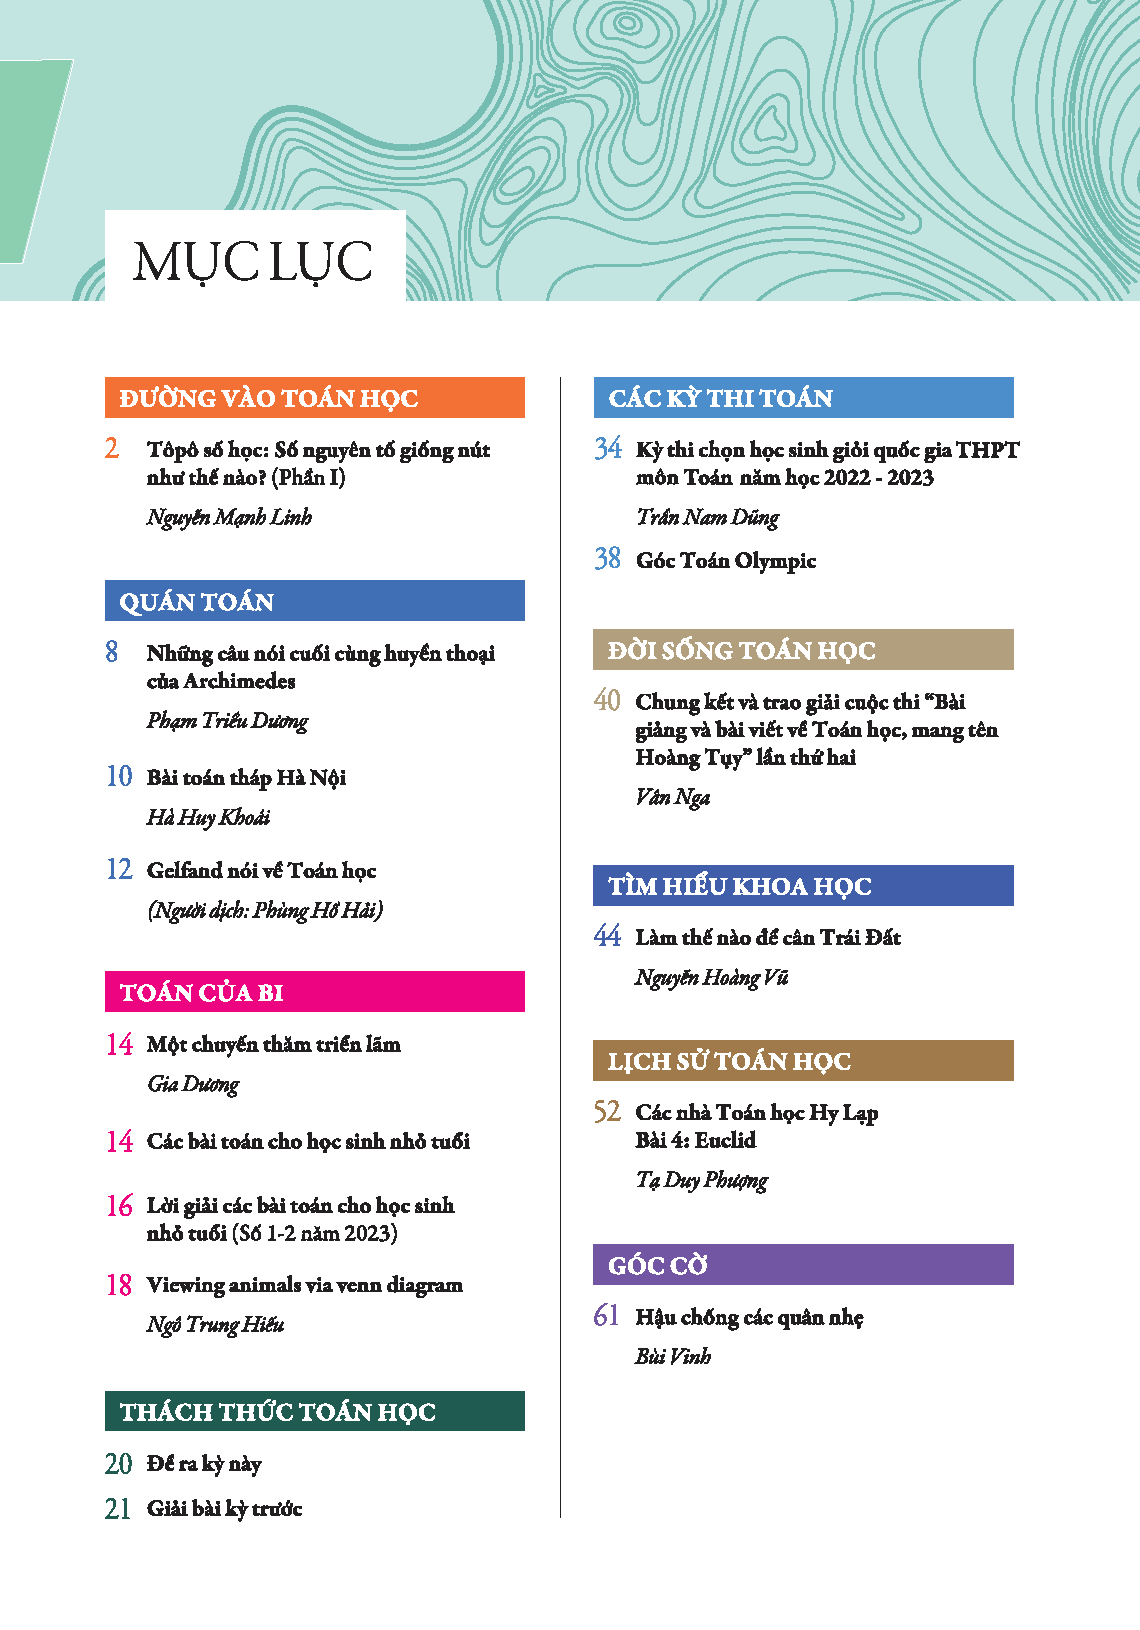
\includegraphics[scale=1]{ML.pdf}}}
%	 \centering
%	 \vspace*{0cm}
%	 \endgroup
%	 \newpage	  
%	 \pagestyle{empty}

%	\setcounter{page}{2}
%	\setcounter{figure}{0}
%	\thispagestyle{duongvaotoanhocnone}
\pagestyle{duongvaotoanhoc}
\everymath{\color{duongvaotoanhoc}}
\graphicspath{{../duongvaotoanhoc/pic/}}
\blfootnote{$^1$\color{duongvaotoanhoc}Universit\'e Paris--Saclay.}
\begingroup
\AddToShipoutPicture*{\put(0,616){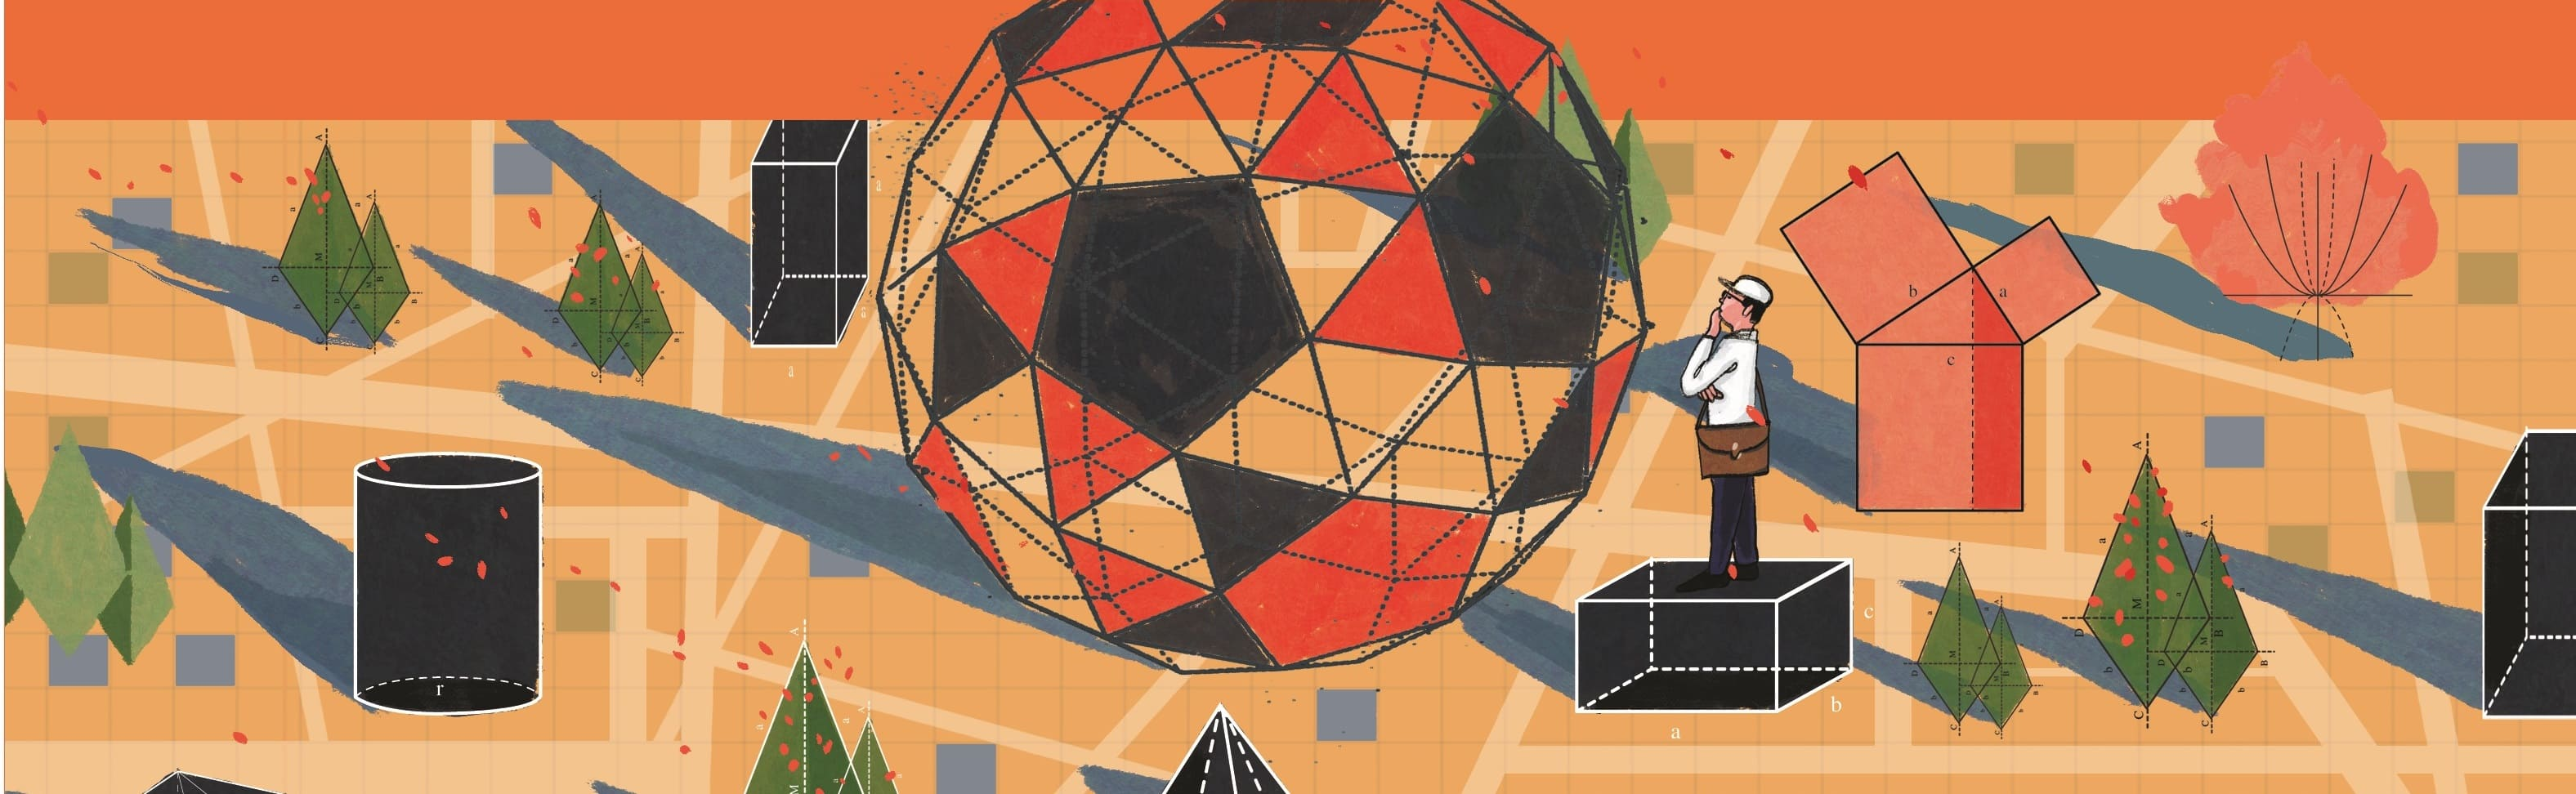
\includegraphics[width=19.3cm]{../bannerduongvao}}}
\AddToShipoutPicture*{\put(58,525){
\includegraphics[scale=1]{../tieude.pdf}}}
\centering
\endgroup
\vspace*{180pt}

\begin{multicols}{2}	
	\textbf{\color{duongvaotoanhoc}Lược đồ}
	\vskip 0.1cm
	Bây giờ, hãy dạo qua thế giới hình học đại số một chút. Với ý tưởng tiên phong của Descartes là nghiên cứu các đối tượng hình học bằng các hệ tọa độ và phương trình đa thức, người ta đã dần dần phát triển hình học đại số. Khác với những người bạn bên tôpô học, các nhà hình học đại số nghiên cứu các đối tượng cứng nhắc hơn: tập nghiệm của các hệ phương trình đa thức. Sau một thời gian, giới toán học nhận ra rằng các trực giác hình học thường mang đến các chứng minh không chặt chẽ và đặc biệt là không giúp gì được ở số chiều cao hơn. Họ đã chuyển sang dùng đại số giao hoán làm công cụ chính để nghiên cứu hình học. Grothendieck, nhà toán học được công nhận rộng rãi là có ảnh hưởng nhất thế kỷ XX, đã cách mạng hóa hình học đại số một lần nữa bằng định nghĩa {\bf\color{duongvaotoanhoc} lược đồ}.
	\vskip 0.1cm
	Ta quay lại với khái niệm trường. Nếu bỏ qua việc luôn làm được phép chia, ta thu được khái niệm {\bf\color{duongvaotoanhoc} vành}. Chẳng hạn, $\mathbb{Z}$ và $\mathbb{Z}/n\mathbb{Z}$ là các vành (phép cộng và phép nhân được hiểu theo nghĩa hiển nhiên). Chú ý rằng ta vẫn yêu cầu làm được phép trừ, nên $\mathbb{N}$ không phải là một vành. Với mỗi vành $R$, ta xây dựng được một không gian tôpô $\text{Spec}(R)$, được gọi là {\bf\color{duongvaotoanhoc} phổ} của $R$. Nếu chỉ nhìn $\text{Spec}(R)$ như một không gian thì ta mất rất nhiều thông tin. Chẳng hạn, phổ của một trường luôn là một điểm. Vì thế, người ta đã làm giàu $\text{Spec}(R)$ một cấu trúc gọi là {\bf\color{duongvaotoanhoc} bó}, chúng làm cho $\text{Spec}(R)$ trở thành một lược đồ.
	\vskip 0.1cm
	Cũng như việc người ta quan tâm đến các hàm liên tục giữa các không gian tôpô, trong hình học đại số người ta quan tâm đến các {\bf\color{duongvaotoanhoc} cấu xạ} giữa các lược đồ. Một cấu xạ $\text{Spec}(R) \to \text{Spec}(S)$ đơn giản được cho bởi một {\bf\color{duongvaotoanhoc} đồng cấu vành} theo chiều ngược lại $f: S \to R$, đồng cấu ở đây nghĩa là $f(x+y) = f(x)+f(y)$, $f(xy) = f(x)f(y)$ và $f(1) = 1$. Chẳng hạn, $\mathbb{Z}$ là một vành con của $\mathbb{Q}$, và phép bao hàm $\mathbb{Z} \to \mathbb{Q}$ cho ta một cấu xạ $\text{Spec}(\mathbb{Q}) \to \text{Spec}(\mathbb{Z})$. Về mặt tôpô thì $\text{Spec}(\mathbb{Q})$ chỉ có một điểm, nên ảnh của cấu xạ này là một điểm của $\text{Spec}(\mathbb{Z})$, được gọi là {\bf\color{duongvaotoanhoc} điểm tổng quát}. Với mỗi số nguyên tố $p$, phép lấy dư modulo $p: \mathbb{Z} \to \mathbb{F}_p$ cho ta một cấu xạ $\text{Spec}(\mathbb{F}_p) \to \text{Spec}(\mathbb{Z})$, đó là một {\bf\color{duongvaotoanhoc} điểm đóng}. Các điểm đóng này và điểm tổng quát tạo nên không gian $\text{Spec}(\mathbb{Z})$. Khác với các không gian Euclid, tôpô trên lược đồ $\text{Spec}(\mathbb{Z})$ rất thô: điểm tổng quát là một điểm nhưng lại trù mật trong cả không gian (người ta hay nói ``điểm tổng quát là điểm nằm ở mọi nơi, nhưng không nằm cụ thể ở đâu cả'').
	\vskip 0.1cm
	Quay lại với lý thuyết không gian phủ. Khi áp dụng nó cho lược đồ, ta không thể chỉ xét khía cạnh tôpô ngây thơ được. Ta muốn $\text{Spec}(\mathbb{F}_p)$ giống với đường tròn $\mathbb{S}^1$, nhưng $\text{Spec}(\mathbb{F}_p)$ lại chỉ có một điểm. Vấn đề với không gian tôpô $\text{Spec}(R)$ là nó có quá ít lân cận, mỗi lân cận đều quá lớn. Cách khắc phục là sáng tạo ra một khái niệm tôpô mới dùng được cho các lược đồ (thứ mà ngày nay gọi là tôpô Grothendieck), với các ``lân cận'' mới. Một trong những loại tôpô đủ mạnh để phân biệt các ``không gian 1 điểm'' $\text{Spec}(K)$ (với $K$ là các trường) là {\bf\color{duongvaotoanhoc} tôpô étale}. Từ ``étale'' được lấy từ văn học Pháp, mang nghĩa nôm na là trạng thái dịu dàng của biển. Với công cụ mới này, người ta định nghĩa được khái niệm nhóm cơ bản étale của lược đồ. Chẳng hạn, nhóm cơ bản étale của $\text{Spec}(\mathbb{F}_p)$ là một nhóm có cùng họ hàng với $\mathbb{Z}$, gọi là ``$\mathbb{Z}$ mũ''. Điều này giải thích vì sao việc coi $\text{Spec}(\mathbb{F}_p)$ như đường tròn $\mathbb{S}^1$ là hợp lý. Tương tự, khái niệm phủ trong thế giới lược đồ phải được hiểu là phủ étale. Đối với các trường, một phủ étale của $\text{Spec}(K)$ đơn giản là $\text{Spec}(L)$, với $L/K$ là một mở rộng bậc hữu hạn. Như vậy, dù $\text{Spec}(K)$ về mặt tôpô chỉ một $1$ điểm, nó lại có nhóm cơ bản étale không tầm thường, hay có rất nhiều phủ. 
	\vskip 0.1cm
	Thực ra khái niệm mở rộng trường và mở rộng vành còn cho ta thêm một chút bên phía tôpô, nó ứng với khái niệm {\bf\color{duongvaotoanhoc} phủ phân nhánh}. Nói nôm na, một phủ phân nhánh bậc $n$ là một hàm liên tục $p: Y \to X$ sao cho nếu bỏ đi một số hữu hạn điểm của $X$ (và các điểm của $Y$ nằm trên chúng) thì ta thu được một phủ $n$-tờ. Các điểm bỏ đi kia (cùng các điểm nằm trên) gọi là các {\bf\color{duongvaotoanhoc} điểm rẽ nhánh} của $p$. Hiện tượng rẽ nhánh là phiên bản hình học của hiện tượng ``nghiệm bội'' trong đại số. Ta xét ví dụ khi $Y$ là đường cong elliptic cho bởi phương trình $y^2=x(x-1)(x-2)$ trong $\mathbb{C}^2$ và $X = \mathbb{C}$. Lấy $p$ là phép chiếu lên trục hoành, $p(x,y) = x$. Khi bỏ đi các điểm $0, 1, 2$ khỏi $X$ (và các điểm $(0,0), (1,0), (2,0)$ khỏi $Y$), ta thu được một phủ $2$--tờ: với mỗi $x \neq 0,1,2$ thì phương trình $y^2=x(x-1)(x-2)$ có hai nghiệm phức phân biệt. Ở các điểm $0, 1, 2$ xảy ra hiện tượng rẽ nhánh, phương trình $y^2=0$ có nghiệm kép $y=0$. Ta nói rằng {\bf\color{duongvaotoanhoc} chỉ số rẽ nhánh} của $p$ tại các điểm $(0,0)$, $(1,0)$, $(2,0)$ bằng $2$.
	\vskip 0.1cm
	\textbf{\color{duongvaotoanhoc}Lý thuyết số đại số}
	\vskip 0.1cm
	Để tìm hiểu các phủ (étale) phân nhánh của lược đồ $\text{Spec}(\mathbb{Z})$, ta bắt đầu từ điểm tổng quát: Phủ étale của $\text{Spec}(\mathbb{Q})$ thì có dạng $\text{Spec}(K)$, với $K = \mathbb{Q}(\alpha)$, và $\alpha$ là nghiệm của một đa thức bậc $n$ bất khả quy với hệ số hữu tỷ. Số $\alpha$ như vậy được gọi là một {\bf\color{duongvaotoanhoc} số đại số}, chẳng hạn $\sqrt{2}, \sqrt[3]{2}, \frac{1 + \sqrt{-3}}{2}$ là các số đại số. Trường $K$ được gọi là một {\bf\color{duongvaotoanhoc} trường số}, và mọi phần tử của nó đều là số đại số. Ta muốn thứ gì đó trong $K$ đóng vai trò như các số nguyên đối với số hữu tỷ. Đó là các {\bf\color{duongvaotoanhoc} số nguyên đại số}. Chúng là những phần tử của $K$ mà là nghiệm của một đa thức với hệ số nguyên và hệ số đầu bằng $1$. Chẳng hạn $\sqrt{2}$ là một số đại số vì nó là nghiệm của $x^2 - 2$. $\frac{1 + \sqrt{5}}{2}$ cũng là một số nguyên đại số (dù trông không có vẻ vậy) vì nó là nghiệm của $x^2-x-1$. Các số nguyên đại số trong $K$ tạo thành một vành $\mathcal{O}$. Việc chuyển từ $\mathbb{Z}$ sang $\mathcal{O}$ là chuyển từ lý thuyết số sơ cấp sang lý thuyết số đại số. Một bài tập đơn giản (bằng cách dùng phân tích duy nhất ra thừa số nguyên tố) là: Các số nguyên đại số trong $\mathbb{Q}$ chính là các số nguyên theo nghĩa cổ điển.
	\vskip 0.1cm
	Lý thuyết số đại số xuất phát từ nỗ lực chứng minh định lý lớn Fermat của Cauchy, Lamé... Ý tưởng như sau: với phương trình $x^2 + y^2 = z^2$ chẳng hạn, ta giải bằng cách đưa về $x^2=z^2-y^2=(z-y)(z+y)$, sau đó lập luận (với phân tích duy nhất ra thừa số nguyên tố) rằng $z-y$ và $z+y$ phải là các số chính phương. Bây giờ, xét phương trình $x^p+y^p=z^p$, với p là số nguyên tố lẻ (dễ thấy ta chỉ cần xét trường hợp này). Để phân tích triệt để $z^p-y^p$ thành các nhân tử bậc nhất, ta buộc phải dùng căn bậc $p$ phức của $1$. Gọi nó là $\zeta = \cos(\frac{2\pi}{p})+i \cdot \sin(\frac{2\pi}{p})$. Thế thì $\zeta$ là một số nguyên đại số (nghiệm của phương trình $x^p - 1$). Và như vậy ta đưa về chứng minh rằng phương trình trên không có nghiệm trong vành mới $\mathbb{Z}[\zeta]$, vành các số nguyên đại số của $\mathbb{Q}(\zeta)$. Sơ hở của cách tiếp cận này là lập luận như trong trường hợp $p=2$ không còn đúng nữa, vì nói chung không có phân tích duy nhất ra thừa số nguyên tố trong $\mathbb{Z}[\zeta]$.
	\vskip 0.1cm
	Một ví dụ về sự không tồn tại của phân tích duy nhất là trường số $K = \mathbb{Q}(\sqrt{-5})$. Vành số nguyên đại số của nó là $\mathcal{O} = \mathbb{Z}[\sqrt{-5}]$, gồm các số có dạng $a+b\sqrt{-5}$ với $a,b \in \mathbb{Z}$. Số $6$ có thể phân tích thành $6 = 2 \cdot 3 = (1+\sqrt{-5}) \cdot (-\sqrt{-5})$. Để thấy rằng hai phân tích này là triệt để và thực sự khác nhau, ta định nghĩa {\bf\color{duongvaotoanhoc} chuẩn} của một số $a+b\sqrt{-5}$ bởi $N(a+b\sqrt{-5}) = a^2 + 5b^2$. Đây là một số tự nhiên, và ta thấy ngay rằng $N(xy) = N(x)N(y)$. Trong phân tích $6 = 2 \cdot 3 = (1+\sqrt{-5}) \cdot (-\sqrt{-5})$, ta có $N(2) = 4, N(3) = 9, N(1+\sqrt{-5}) = N(1-\sqrt{-5}) = 6$, nên các nhân tử xuất hiện ở hai phân tích thực sự khác nhau.  Ngoài ra, về cơ bản ta không thể phân tích thêm được nữa, vì không có phần tử nào có chuẩn bằng $2$ hoặc $3$ (một tính toán số học đơn giản cho thấy rằng phương trình các $a^2 + 5b^2 = 2$ và $a^2 + 5b^2 = 3$ đều không có nghiệm nguyên). Điều này cho thấy sự thiếu sót của phân tích duy nhất ra thừa số nguyên tố trong $\mathbb{Z}[\sqrt{-5}]$.
	\vskip 0.1cm
	Sự sụp đổ của phân tích duy nhất trong $\mathcal{O}$ đã chấm dứt hi vọng chứng minh định lý lớn Fermat bằng lý thuyết số đại số cổ điển. Dù vậy, vành $\mathcal{O}$ vẫn giữ được một tính chất của vành $\mathbb{Z}$; nó là một {\bf\color{duongvaotoanhoc} vành Dedekind}. Thay vì phân tích duy nhất của các số, người ta định nghĩa khái niệm {\bf\color{duongvaotoanhoc} số lý tưởng} (cái mà ngày nay gọi là {\bf\color{duongvaotoanhoc} iđêan}). Đại khái nó là thứ gì đó cho phép nói về quan hệ chia hết cũng như làm phép nhân. Việc $\mathcal{O}$ là vành Dedekind có nghĩa là mọi số lý tưởng đều phân tích một cách duy nhất ra các số lý tưởng nguyên tố. Một số nguyên đại số $a \in \mathcal{O}$ định nghĩa một số lý tưởng $(a)$, được gọi là một số lý tưởng chính. Hai số $a$ và $b$ định nghĩa cùng một số lý tưởng nếu chúng {\bf\color{duongvaotoanhoc} liên kết}, nghĩa là $a|b$ đồng thời $b|a$. Nói riêng, nếu là $u|1$ thì $(u) = (1)$. Nếu tất cả số lý tưởng nguyên tố đều có dạng trên thì $\mathcal{O}$ có phân tích duy nhất của các số (thực sự). Điều này không đúng trong $\mathbb{Z}[\sqrt{-5}]$; cụ thể là khi phân tích $(6) = (2) \cdot (3) = (1 + \sqrt{-5}) \cdot (1 - \sqrt{-5})$, ta vẫn phân tích được tiếp: $(2) = \mathfrak{p}_1\mathfrak{p}_2$, $(3) = \mathfrak{p}_3\mathfrak{p}_4$, $(1 + \sqrt{-5}) = \mathfrak{p}_1\mathfrak{p}_3$, $(1 - \sqrt{-5}) = \mathfrak{p}_2\mathfrak{p}_4$, trong đó $\mathfrak{p}_1, \mathfrak{p}_2, \mathfrak{p}_3, \mathfrak{p}_4$ là các số lý tưởng nguyên tố {\it không chính}. Chuẩn của chúng lần lượt là $N(\mathfrak{p}_1) = N(\mathfrak{p}_2) = 2$ và $N(\mathfrak{p}_3) = N(\mathfrak{p}_4) = 3$. Như vậy ta có phân tích duy nhất của $(6)$ thành các số lý tưởng.
	\vskip 0.1cm
	Cũng như mỗi số nguyên tố $p$ ứng với các điểm đóng $\text{Spec}(\mathbb{F}_p) \to \text{Spec}(\mathbb{Z})$, mỗi số lý tưởng nguyên tố $\mathfrak{p}$ trong trong $\mathcal{O}$ cho ta một trường hữu hạn $\mathbb{F}_{\mathfrak{p}}$ (gọi là {\bf\color{duongvaotoanhoc} trường thặng dư} của $\mathfrak{p}$), cùng một điểm đóng $\text{Spec}(\mathbb{F}_{\mathfrak{p}}) \to \text{Spec}(\mathcal{O})$. Cùng với điểm tổng quát $\text{Spec}(K)$, chúng tạo thành lược đồ $\text{Spec}(\mathcal{O})$. Vì $\mathbb{Z}$ là một vành con của $\mathcal{O}$, ta có một cấu xạ $\text{Spec}(\mathcal{O}) \to \text{Spec}(\mathbb{Z})$, một phủ étale phân nhánh. Mỗi số nguyên tố $p$ trong $\mathbb{Z}$ có thể không còn là số lý tưởng nguyên tố trong $\mathcal{O}$, nó phân rã thành tích của một số hữu hạn số lý tưởng nguyên tố, $(p) = \mathfrak{p_1}\mathfrak{p_2}\cdots\mathfrak{p_n}$. Các số lý tưởng nguyên tố xuất hiện trong phân tích trên chính xác là những điểm của $\text{Spec}(\mathcal{O})$ nằm trên điểm đóng của $\text{Spec}(\mathbb{Z})$ ứng với $p$. Hiện tượng phân nhánh nhánh xảy ra nếu có một số lý tưởng $\mathfrak{p}_i$ xuất hiện nhiều lần trong phân tích trên, ta gọi đó số lần đó là {\bf\color{duongvaotoanhoc} chỉ số rẽ nhánh} của $\mathfrak{p}_i$, nó đóng vai trò như chỉ số rẽ nhánh trong tôpô cổ điển.
	\vskip 0.1cm
	Một bất đẳng thức trong lý thuyết số đại số, {\it chặn Minkowski}, cho phép xác định cụ thể phân tích trên. Hơn thế nữa, nó còn cho ta biết chính xác khi nào thì một số nguyên tố $p$ rẽ nhánh trong $\mathcal{O}$. Một hệ quả của nó là với mọi trường số $K$, luôn có ít nhất một số nguyên tố $p$ rẽ nhánh trong vành $\mathcal{O}$ các số nguyên đại số trong $K$, nghĩa là $\text{Spec}(\mathbb{Z})$ không có phủ  étale không rẽ nhánh nào ngoài phủ tầm thường (cho bởi ánh xạ đồng nhất $\mathbb{Z} \to \mathbb{Z}$), hay nó là đơn liên.
	\vskip 0.1cm
	\textbf{\color{duongvaotoanhoc}Nút}
	\vskip 0.1cm
	Trong thế giới của các không gian tôpô thì có rất nhiều không gian đơn liên, và ta muốn tìm cái nào giống với $\text{Spec}(\mathbb{Z})$. Sự đột phá nằm ở các phát hiện sau đây của Mumford, Manin, và sau này là Mazur. Ở phía tôpô, các khái niệm điểm ($0$--chiều), đường ($1$--chiều), mặt ($2$--chiều) được tổng quát lên thành các đa tạp. Một đa tạp $3$--chiều là một không gian tôpô mà nhìn địa phương thì giống như không gian Euclid $\mathbb{R}^3$ (cũng như bề mặt trái đất là một đa tạp $2$--chiều, nhìn địa phương thì giống như mặt phẳng).
	\vskip 0.1cm
	Bên cạnh nhóm cơ bản, tôpô đại số cổ điển còn cung cấp các bất biến đại số khác cho các không gian tôpô, gọi là các {\bf\color{duongvaotoanhoc} nhóm đồng điều}. Nhóm đồng điều bậc $n$ của một đa tạp $X$ được xây dựng như sau: Xét các tổ hợp tạo thành từ một số đa tạp con $n$--chiều (chúng được gọi là các {\bf\color{duongvaotoanhoc} $n$-dây chuyền}). Nếu chúng tạo thành một vòng kín, ta gọi nó là một {\bf\color{duongvaotoanhoc} $n$--chu trình}. Nếu nó tạo thành biên của một đa tạp con $(n+1)$--chiều, ta gọi nó là một {\bf\color{duongvaotoanhoc} $n$--biên}. Một $n$--biên thì luôn là một $n$--chu trình. Nhóm $H_n(X)$ được định nghĩa là chênh lệch giữa các nhóm các $n$--chu trình và nhóm các $n$--biên: một $n$--chu trình mà không phải $n$--biên thì nó bao quanh một ``lỗ thủng'' $(n+1)$--chiều; như vậy các nhóm đồng điều phát hiện các lỗ thủng trên $X$. Phiên bản đối ngẫu của đồng điều là {\bf\color{duongvaotoanhoc} đối đồng điều}, các nhóm $H^n(X)$. Về cơ bản thì chúng cũng phát hiện các lỗ thủng. Về mặt kỹ thuật thì chúng dễ tính toán hơn đồng điều một chút, đồng thời có nhiều cấu trúc hơn. {\it Đối ngẫu Poincaré} nói rằng nếu $X$ là một đa tạp đóng, khả định hướng, $d$--chiều, thì ta có một đối ngẫu hoàn hảo giữa hai nhóm $H^{d-i}(X)$ và $H^i(X)$ với mỗi $i = 0,1,\ldots,d$.
	\vskip 0.1cm
	Với các lược đồ, các nhóm đối đồng điều nhìn chung không cho thông tin gì (phần lớn chúng bằng $0$) khi ta tính theo tôpô thông thường. Một lần nữa nhờ công của Grothendieck, ta có thể tính {\bf\color{duongvaotoanhoc}đối đồng điều étale}.  Trên một trường, chúng được gọi là {\bf\color{duongvaotoanhoc}đối đồng điều Galois}, một công cụ đã được dùng từ lâu trước đó trong số học. Với các trường hữu hạn, đối đồng điều Galois của chúng rất đơn giản, chúng khác $0$ ngoài bậc $0$ và $1$, và ta có một đối ngẫu hoàn hảo giữa các nhóm đối đồng điều ở hai bậc này. Điều này tương tự với đối ngẫu Poincaré cho các đa tạp $1$--chiều, khẳng định thêm niềm tin rằng phổ của trường hữu hạn là phiên bản đại số của đường tròn. 
	\vskip 0.1cm
	Đối với các lược đồ $\text{Spec}(\mathcal{O})$, với $\mathcal{O}$ là vành số nguyên đại số của một trường số $K$ nào đó, các nhóm đối đồng điều étale thỏa mãn đối ngẫu giữa bậc $0$ và bậc $3$ cũng như bậc $1$ và bậc $2$. Các kết quả này được gọi là {\it đối ngẫu Artin--Verdier}, được khám phá khi áp dụng đối đồng điều étale cho lý thuyết trường các lớp toàn cục, một phần của lý thuyết số. Điều này gợi cho ta rằng phiên bản tôpô của $\text{Spec}(\mathcal{O})$ ``nên" là các đa tạp $3$--chiều. Vậy $\text{Spec}(\mathbb{Z})$ ứng với đa đạp đóng $3$--chiều nào? Ta thấy ở trên rằng $\text{Spec}(\mathbb{Z})$ đơn liên, và đa tạp đóng $3$--chiều đơn liên thì chỉ có thể đồng phôi với mặt (siêu) cầu  $\mathbb{S}^3$! Đó là nội dung của {\it giả thuyết Poincaré}, bài toán duy nhất đã được giải trong $7$ bài toán thiên niên kỷ. Tác giả của lời giải, thiên tài lập dị Perelman, đã từ chối cả Huy chương Fields lẫn Giải thưởng Thiên niên kỷ (Millennium Prize) cho công trình vô song của mình.
	\vskip 0.1cm
	Sau khi bỏ ra rất nhiều công sức, ta đã thấy được cầu nối mong manh giữa tôpô học và số học, rằng phiên bản số học của $\mathbb{S}^1$ là (phổ của) một trường hữu hạn, và của một đa tạp đóng $3$--chiều là vành các số nguyên đại số của một trường số. Bây giờ là lúc chúng ta thu hoạch kết quả, chiêm ngưỡng những sự tương tự đáng ngạc nhiên dựa trên cầu nối này. Một số lý tưởng nguyên tố $\mathfrak{p}$ trong $\mathcal{O}$ cho ta một phép nhúng $\text{Spec}(\mathbb{F}_\mathfrak{p}) \hookrightarrow \text{Spec}(\mathcal{O})$. Về phía tôpô, ta xét các phép nhúng $\mathbb{S}^1 \hookrightarrow M$, với $M$ là một đa tạp (đóng, khả định hướng) $3$-chiều. Chúng được gọi là các {\bf\color{duongvaotoanhoc} nút} trong $M$. Nói riêng, phiên bản tôpô của mỗi số nguyên tố $p$ (với phép nhúng tương ứng $\text{Spec}(\mathbb{F}_p) \hookrightarrow \text{Spec}(\mathbb{Z})$) là một nút trong $\mathbb{S}^3$ (ta sẽ tập trung vào các nút này). Từ một định lý sâu sắc trong tôpô học, {\it định lý Borsuk--Ulam}, ta có thể chỉ ra rằng một phép nhúng như thế không thể là toàn ánh, nghĩa là ta có thể xem một nút như một phép nhúng từ $\mathbb{S}^1$ vào $\mathbb{S}^3$ bỏ đi một điểm, nói cách khác chính là không gian Euclid $\mathbb{R}^3$.
	\vskip 0.1cm
	Để biểu diễn một nút $K: \mathbb{S}^1 \hookrightarrow \mathbb{R}^3$ ta có thể chiếu nó lên một mặt phẳng sau cho tại mỗi điểm giao nhau chỉ có đúng $2$ đường đi qua. Chúng ứng với một {\bf\color{duongvaotoanhoc} sợi trên} và một {\bf\color{duongvaotoanhoc} sợi dưới}, ta biểu diễn sợi dưới bằng nét đứt tại giao điểm đó.  Đó là một {\bf\color{duongvaotoanhoc} biểu đồ phẳng} của nút.
	\begin{figure}[H]
		\vspace*{-5pt}
		\centering
		\captionsetup{labelformat= empty, justification=centering}
		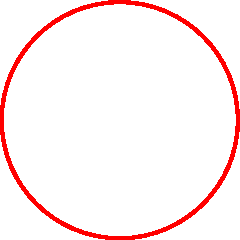
\includegraphics[width= 0.28\linewidth]{unknot.pdf}\quad
		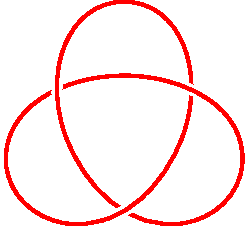
\includegraphics[width= 0.28\linewidth]{trefoil.pdf}\quad
		
\includegraphics[width= 0.28\linewidth]{figure 8.pdf}
		\caption{\small\textit{\color{duongvaotoanhoc}Hình $10$: Biểu đồ phẳng của nút tầm thường, nút ba lá, và nút số $8$.}}
		\vspace*{-10pt}
	\end{figure}
	Tất nhiên, mọi nút đều đồng phôi với $\mathbb{S}^1$. Ta cần cả thông tin về phép nhúng $\mathbb{S}^1 \to \mathbb{R}^3$ để phân biệt các nút với nhau. Các nhà lý thuyết nút gọi sự giống nhau của các nút là {\bf\color{duongvaotoanhoc} đẳng luân}. Một cách trực giác, hai nút đẳng luân nếu ta có thể tháo dỡ một nút rồi buộc thành nút còn lại (mà không cắt được cắt nút ra). Hóa ra, hai nút đẳng luân khi và chỉ khi phần bù của chúng trong $\mathbb{S}^3$ đồng phôi với nhau ({\it định lý Gordon--Luecke}).
	\vskip 0.1cm
	\textbf{\color{duongvaotoanhoc}Từ điển M$^2$KR}
	\vskip 0.1cm
	Từ điển Mazur--Morishita--Kapranov--Reznikov (M$^2$KR) là một danh sách những sự tương tự giữa lý thuyết số và hình học của các đa tạp $3$--chiều; ở đó các số lý tưởng tưởng ứng với các liên kết, các số lý tưởng nguyên tố ứng với các nút. Sau đây là một số tương ứng giữa tôpô và số học trong từ điển này.
	\vskip 0.1cm
	Mỗi số lý tưởng trong $\mathcal{O}$ phân tích thành tích của các số lý tưởng nguyên tố. Phiên bản tôpô của số lý tưởng là {\bf\color{duongvaotoanhoc} liên kết}: một liên kết trong một đa tạp đóng $3$--chiều $M$ là một phép nhúng từ một số hữu hạn bản sao rời rạc của $\mathbb{S}^1$ vào $M$. Các ví dụ về liên kết trong $\mathbb{S}^3$ là {\bf\color{duongvaotoanhoc} liên kết Hopf} và {\bf\color{duongvaotoanhoc} vòng Borromean}, lần lượt được tạo bởi $2$ và $3$ nút tầm thường lồng nhau.
	\begin{figure}[H]
		\vspace*{-15pt}
		\centering
		\captionsetup{labelformat= empty, justification=centering}
		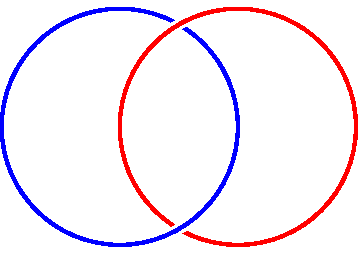
\includegraphics[width= 0.38\linewidth]{hopf.pdf}\quad\quad
		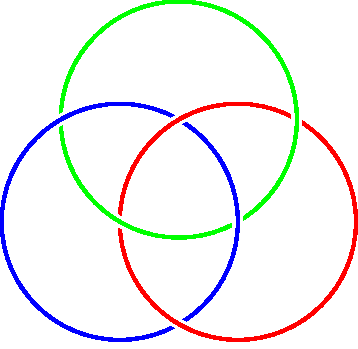
\includegraphics[width= 0.38\linewidth]{borromean.pdf}
		\caption{\small\textit{\color{duongvaotoanhoc}Hình $11$: Biểu đồ phẳng của liên kết Hopf và vòng Borromean.}}
		\vspace*{-10pt}
	\end{figure}
	Để thêm phần thuyết phục rằng tại sao $M$ lại tương ứng với (vành số nguyên đại số) một trường số, ta nhắc đến {\it định lý Alexander}: Mọi đa tạp đóng $3$--chiều đều là một phủ phân nhánh của $\mathbb{S}^3$, trong đó các điểm rẽ nhánh trong $\mathbb{S}^3$ tạo thành một liên kết. Tương tự, một mở rộng $L/K$ của trường số có thể được coi như một phủ phân nhánh giữa hai đa tạp đóng $3$--chiều.
	\vskip 0.1cm
	Một số nguyên đại số $a \in \mathcal{O}$ ứng với một mặt compact $S$ (có thể có biên) nhúng trong đa tạp đóng $3$--chiều $M$. Số lý tưởng chính $(a)$ ứng với biên $\partial S$, đây là một liên kết, và chúng ứng với các $1$--đối biên, tức là phần tử $0$ trong nhóm đồng điều $H_1(M)$. Các số lý tưởng khác tương ứng với các liên kết, chúng là các $1$--chu trình mà không phải biên, đại diện cho các phần tử không tầm thường của $H_1(M)$. Ta biết rằng trong $\mathbb{Z}$ có phân tích duy nhất ra thừa số nguyên tố, hay mọi số lý tưởng nguyên tố đều là số lý tưởng chính. Tương ứng, với $M = \mathbb{S}^3$, ta có $H_1(M) = 0$ (vì $\mathbb{S}^3$ không có lỗ thủng $2$--chiều nào), nghĩa là mọi liên kết đều là biên của một mặt nào đó. Seifert đã đưa ra một thuật toán khá đơn giản để xây dựng một mặt với biên cho trước. Chẳng hạn, {\bf\color{duongvaotoanhoc} mặt Seifert} của liên kết Hopf chính là {\it mặt M\"obius}.
	\begin{figure}[H]
		\vspace*{-5pt}
		\centering
		\captionsetup{labelformat= empty, justification=centering}
		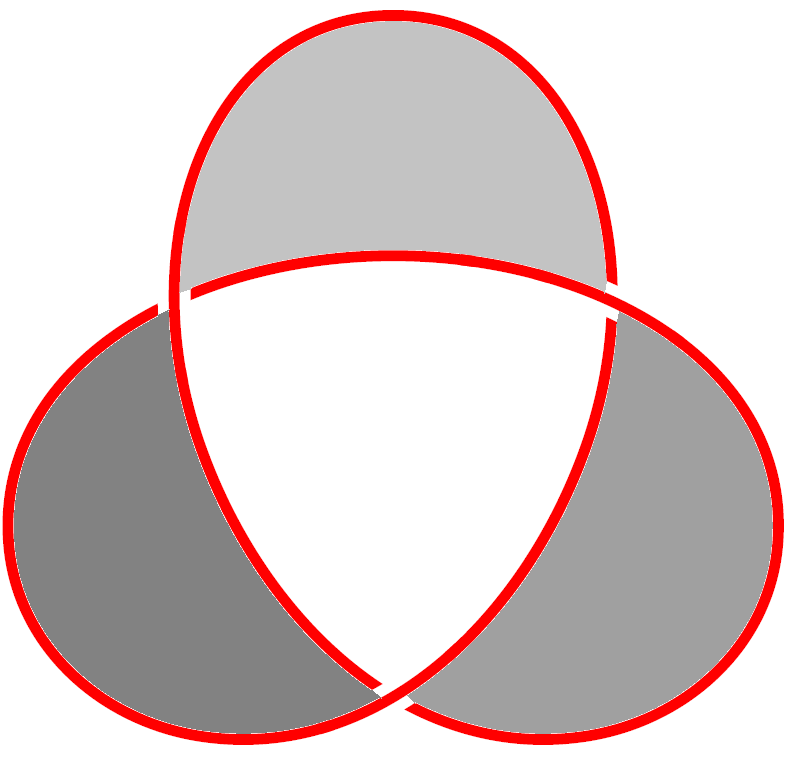
\includegraphics[width= 0.4\linewidth]{seifert1}\quad\quad
		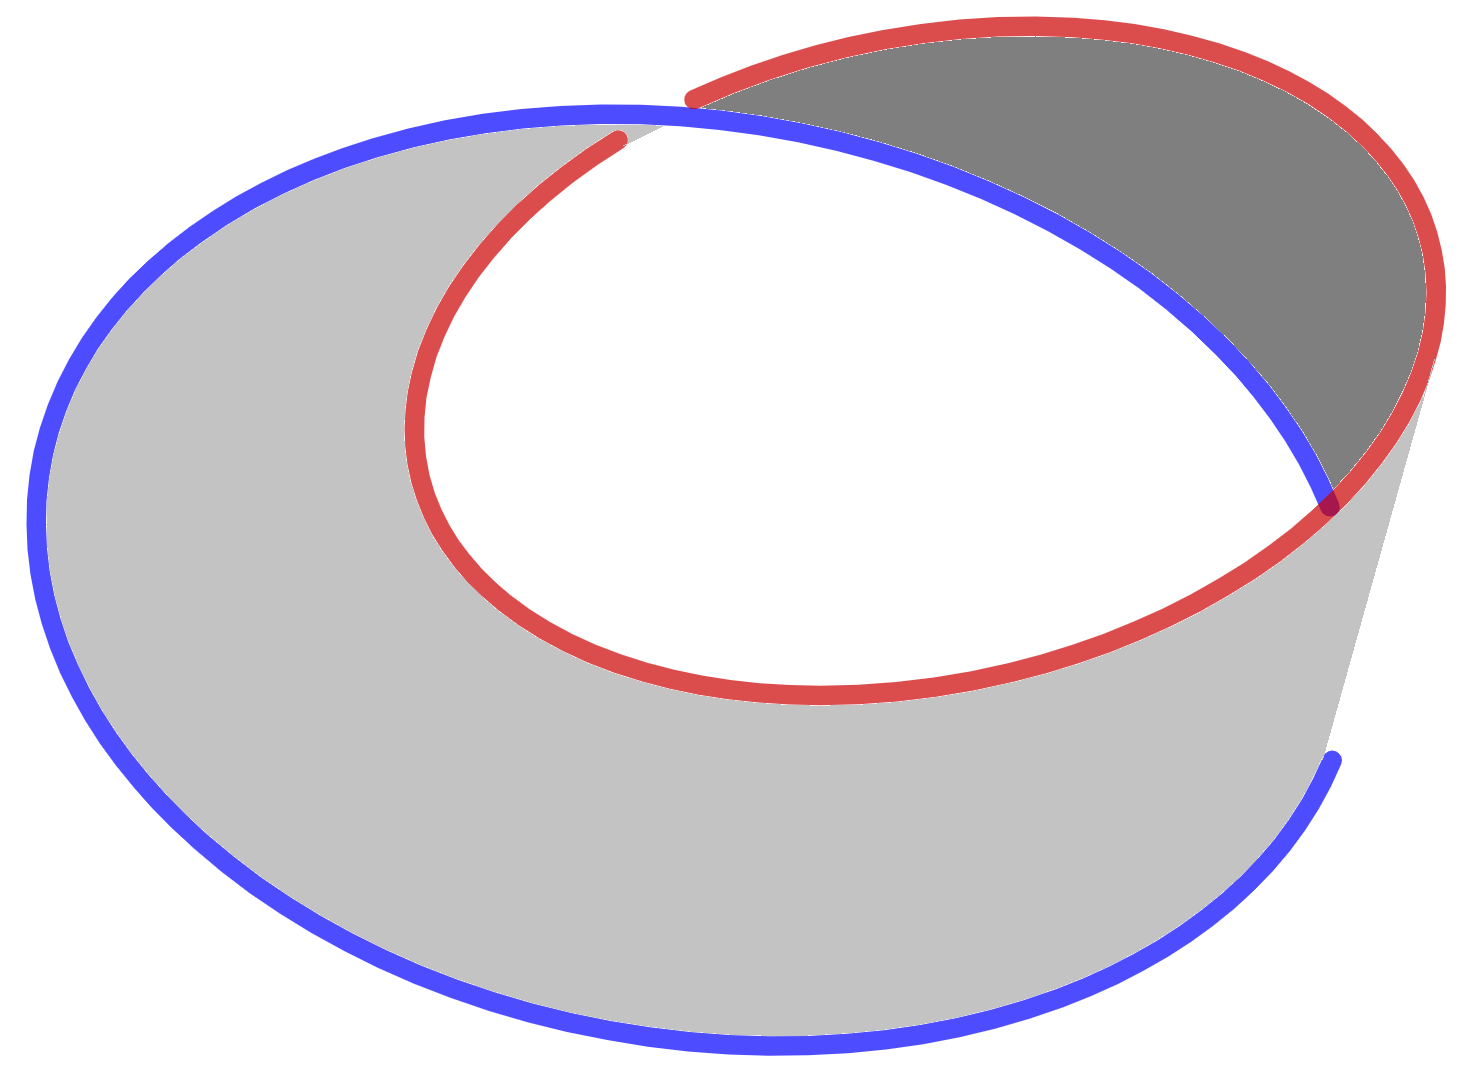
\includegraphics[width= 0.4\linewidth]{seifert2}
		\caption{\small\textit{\color{duongvaotoanhoc}Hình $12$: Mặt Seifert của nút ba lá và của liên kết Hopf (mặt M\"obius).}}
		\vspace*{-10pt}
	\end{figure}
	Sự tương tự tiếp theo: với $p$ là một số nguyên tố, ta xét vành $\mathbb{Z}_p$ các số nguyên $p$--adic cũng như trường $\mathbb{Q}_p$ các số $p$--adic. So với $\text{Spec}(\mathbb{Z})$, phổ $\text{Spec}(\mathbb{Z}_p)$ chỉ còn $2$ điểm là điểm tổng quát $\text{Spec}(\mathbb{Q}_p)$ và điểm đóng $\text{Spec}(\mathbb{F}_p)$, vì thế ta gọi thao tác này {\bf\color{duongvaotoanhoc} địa phương hóa} (tập trung nhìn vào số nguyên tố $p$ và quên đi các số nguyên tố khác). Thao tác này ứng với việc lấy {\bf\color{duongvaotoanhoc} lân cận ống} $V$ của nút, kết quả thu được là một hình xuyến đặc. Dù hình xuyến đặc không đồng phôi với đường tròn, chúng {\bf\color{duongvaotoanhoc} tương đương đồng luân với nhau}, điều này ứng với việc $\text{Spec}(\mathbb{Z}_p)$ và $\text{Spec}(\mathbb{F}_p)$ {\bf\color{duongvaotoanhoc} tương đương đồng luân étale với nhau}. Khi bỏ nút ban đầu khỏi $V$, ta thu được một không gian tương đương đồng luân với mặt xuyến (rỗng). Nhóm cơ bản của mặt xuyến là $\mathbb{Z} \times \mathbb{Z}$, một nhóm được sinh bởi hai phần tử là hai khuyên như trong Hình $13$.
	\begin{figure}[H]
		\vspace*{-5pt}
		\centering
		\captionsetup{labelformat= empty, justification=centering}
		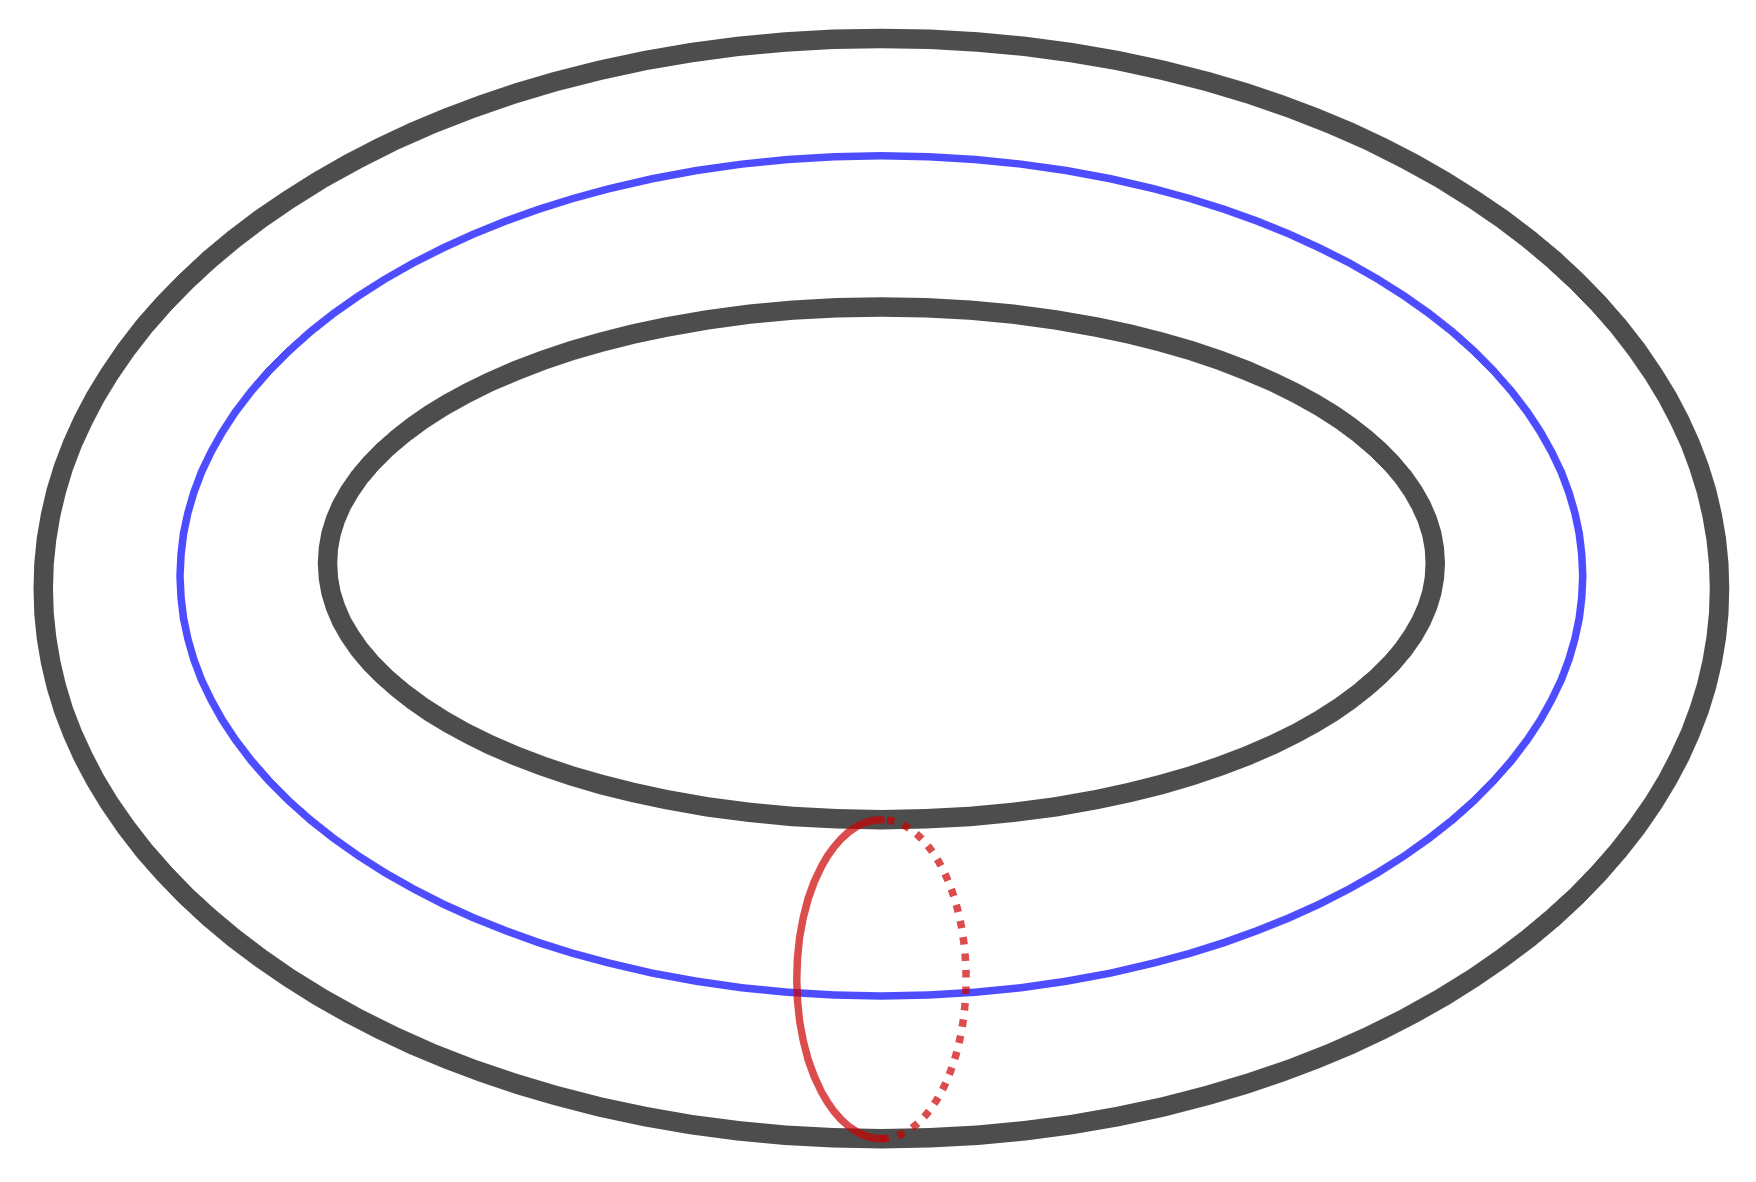
\includegraphics[width= 0.65\linewidth]{h13}
		\caption{\small\textit{\color{duongvaotoanhoc}Hình $13$: Nhóm cơ bản của mặt xuyến được sinh bởi hai khuyên màu xanh và màu đỏ.}}
		\vspace*{-5pt}
	\end{figure}
	Tương ứng, khi bỏ $\text{Spec}(\mathbb{F}_p)$ khỏi $\text{Spec}(\mathbb{Z}_p)$, ta thu được $\text{Spec}(\mathbb{Q}_p)$, và {\bf\color{duongvaotoanhoc} nhóm Galois rẽ nhánh yếu} (một phiên bản nhỏ hơn của nhóm cơ bản étale) của $\mathbb{Q}_p$ cũng được mô tả bởi $2$ phần tử sinh. Sau cùng, lý thuyết trường các lớp địa phương của Tate cho ta các đối ngẫu hoàn hảo giữa đối đồng điều Galois của  $\mathbb{Q}_p$ ở bậc $0$ và bậc $2$, cũng như ở bậc $1$ và chính nó. Tương ứng, ta có đối ngẫu Poincaré cho mặt xuyến, một đa tạp đóng $2$--chiều.
	\vskip 0.1cm
	\textbf{\color{duongvaotoanhoc}Thao tác trên biểu đồ phẳng}
	\vskip 0.1cm
	Quay lại với sự đẳng luân của các nút. Một câu hỏi rất tự nhiên là làm thế nào để chứng minh hai nút không đẳng luân? Đẳng luân vốn là một điều kiện tôpô quá khó sử dụng. Một khó khăn khi sử dụng các biểu đồ phẳng là hai nút đẳng luôn có thể cho hai biểu đồ phẳng trông rất khác nhau. Vậy vấn đề đầu tiên là ta cần tìm cách phân biệt hai nút qua biểu đồ phẳng của chúng (bài toán nhận biết nút). Điều này có thể được thực hiện một cách tổ hợp. Cụ thể, hai biểu đồ phẳng biểu diễn hai nút đẳng luân khi và chỉ khi tồn tại một chuỗi hữu hạn các thao tác thuộc một trong $4$ kiểu, được gọi là các {\bf\color{duongvaotoanhoc} chuyển động Reidemeister}.
	\begin{figure}[H]
		\vspace*{-10pt}
		\centering
		\captionsetup{labelformat= empty, justification=centering}
		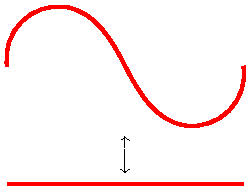
\includegraphics[width= 0.3\linewidth]{R0.pdf}\quad
		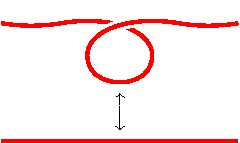
\includegraphics[width= 0.3\linewidth]{R1.pdf}
		\caption{\small\textit{\color{duongvaotoanhoc}R$0$: Phép đẳng luân phẳng.\hspace*{20pt}  RI: Phép xoắn.}}
		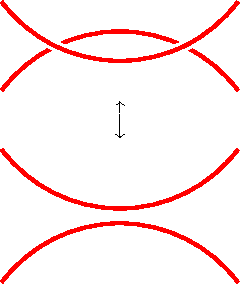
\includegraphics[width= 0.3\linewidth]{R2.pdf}\quad
		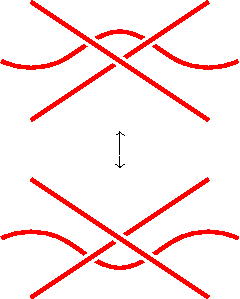
\includegraphics[width= 0.3\linewidth]{R3.pdf}
		\caption{\small\textit{\color{duongvaotoanhoc}RII: Phép đè.\hspace*{30pt} RIII: Phép trượt.}}
		\caption{\small\textit{\color{duongvaotoanhoc}Hình $14$: Các chuyển động Reidemeister.}}
		\vspace*{-10pt}
	\end{figure}
	Từ biểu đồ phẳng của nút, ta dùng các đại lượng không đổi qua các chuyển động Reidemeister, các {\bf\color{duongvaotoanhoc} bất biến nút}. Hai nút có bất biến khác nhau thì phải khác nhau. Một ví dụ như vậy là {\bf\color{duongvaotoanhoc} bất biến tô màu}. Ta nói một biểu đồ phẳng của nút là {\bf\color{duongvaotoanhoc} tô được bằng $\pmb{3}$ màu} nếu mỗi sợi (phần đường cong liên tục giữa hai giao điểm liên tiếp của nút) đều có thể tô được bằng một trong $3$ màu cho trước, sao cho
	\vskip 0.05cm
	$\bullet$ ít nhất hai màu phải được dùng;
	\vskip 0.05cm
	$\bullet$ tại mỗi giao điểm, sợi trên cùng $2$ sợi dưới hoặc là được tô cùng màu, hoặc là được tô $3$ màu khác nhau.
	\vskip 0.05cm
	Ví dụ, nút ba lá hiển nhiên tô được bằng $3$ màu, nút tầm thường hiển nhiên không tô được bằng $3$ màu. Nút số $8$ cũng không tô được bằng $3$ màu. Vậy ít nhất ta biết rằng nút $3$ lá không đẳng luân với nút tầm thường cũng như nút số $8$.
	\vskip 0.05cm
	Hiển nhiên là bất biến tô màu chỉ cho phép phân loại các nút thành $2$ lớp. Ta cần các loại bất biến khác. Ví dụ, xét nút ba lá trái và ảnh gương của nó là nút ba lá phải. Tất nhiên cả hai đều tô được bằng $3$ màu. Rất ngạc nhiên, hai nút này không đẳng luân! Hãy thử dùng các chuyển động Reidemeister để gỡ nút này thành nút kia và bạn sẽ sớm bị thuyết phục. Một bất biến cho phép phân biệt hai nút này là {\bf\color{duongvaotoanhoc} đa thức Alexander}. Đa thức này đến từ {\it lý thuyết Alexander--Fox}, và người ta phát hiện ra phiên bản số học của nó là {\it lý thuyết Iwasawa}. Sự song song của chúng cho phép ta dịch các kết quả từ một bên sang bên còn lại.
	\begin{figure}[H]
		\vspace*{-10pt}
		\centering
		\captionsetup{labelformat= empty, justification=centering}
		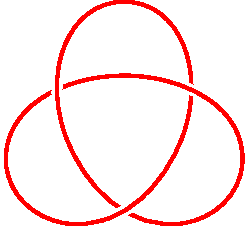
\includegraphics[width= 0.36\linewidth]{trefoil.pdf}\quad\quad
		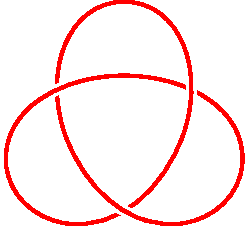
\includegraphics[width= 0.36\linewidth]{mirror trefoil.pdf}
		\caption{\small\textit{\color{duongvaotoanhoc}Hình $15$: Nút ba lá trái và nút ba lá phải.}}
		\vspace*{-10pt}
	\end{figure}
	Một kiểu bất biến khác cho liên kết là {\bf\color{duongvaotoanhoc} số liên kết}. Xét một liên kết được tạo bởi hai nút. Giữa hai nút $L$ và $K$, ta có thể định nghĩa {\bf\color{duongvaotoanhoc} số liên kết} qua biểu đồ phẳng của chúng như sau. Chẳng hạn, tô màu đỏ cho $L$ và màu xanh cho $K$, đồng thời định hướng cho chúng (mỗi nút có thể có $1$ trong $2$ hướng). Tại các điểm trên biểu đồ phẳng mà có một sợi của nút này nằm trên một sợi của nút kia hoặc ngược lại, ta đánh dấu $+$ hoặc $-$ theo quy tắc ở Hình $16$. Sau đó ta lấy số dấu cộng trừ đi số dấu trừ, và lấy kết quả chia đôi. Kết quả cuối cùng thu được được gọi là số liên kết $\text{lk}(L,K)$. Chẳng hạn, số liên kết của hai nút trong liên kết Hopf là $1$ hoặc $-1$, tùy theo cách định hướng hai nút.
	\begin{figure}[H]
		\vspace*{-5pt}
		\centering
		\captionsetup{labelformat= empty, justification=centering}
		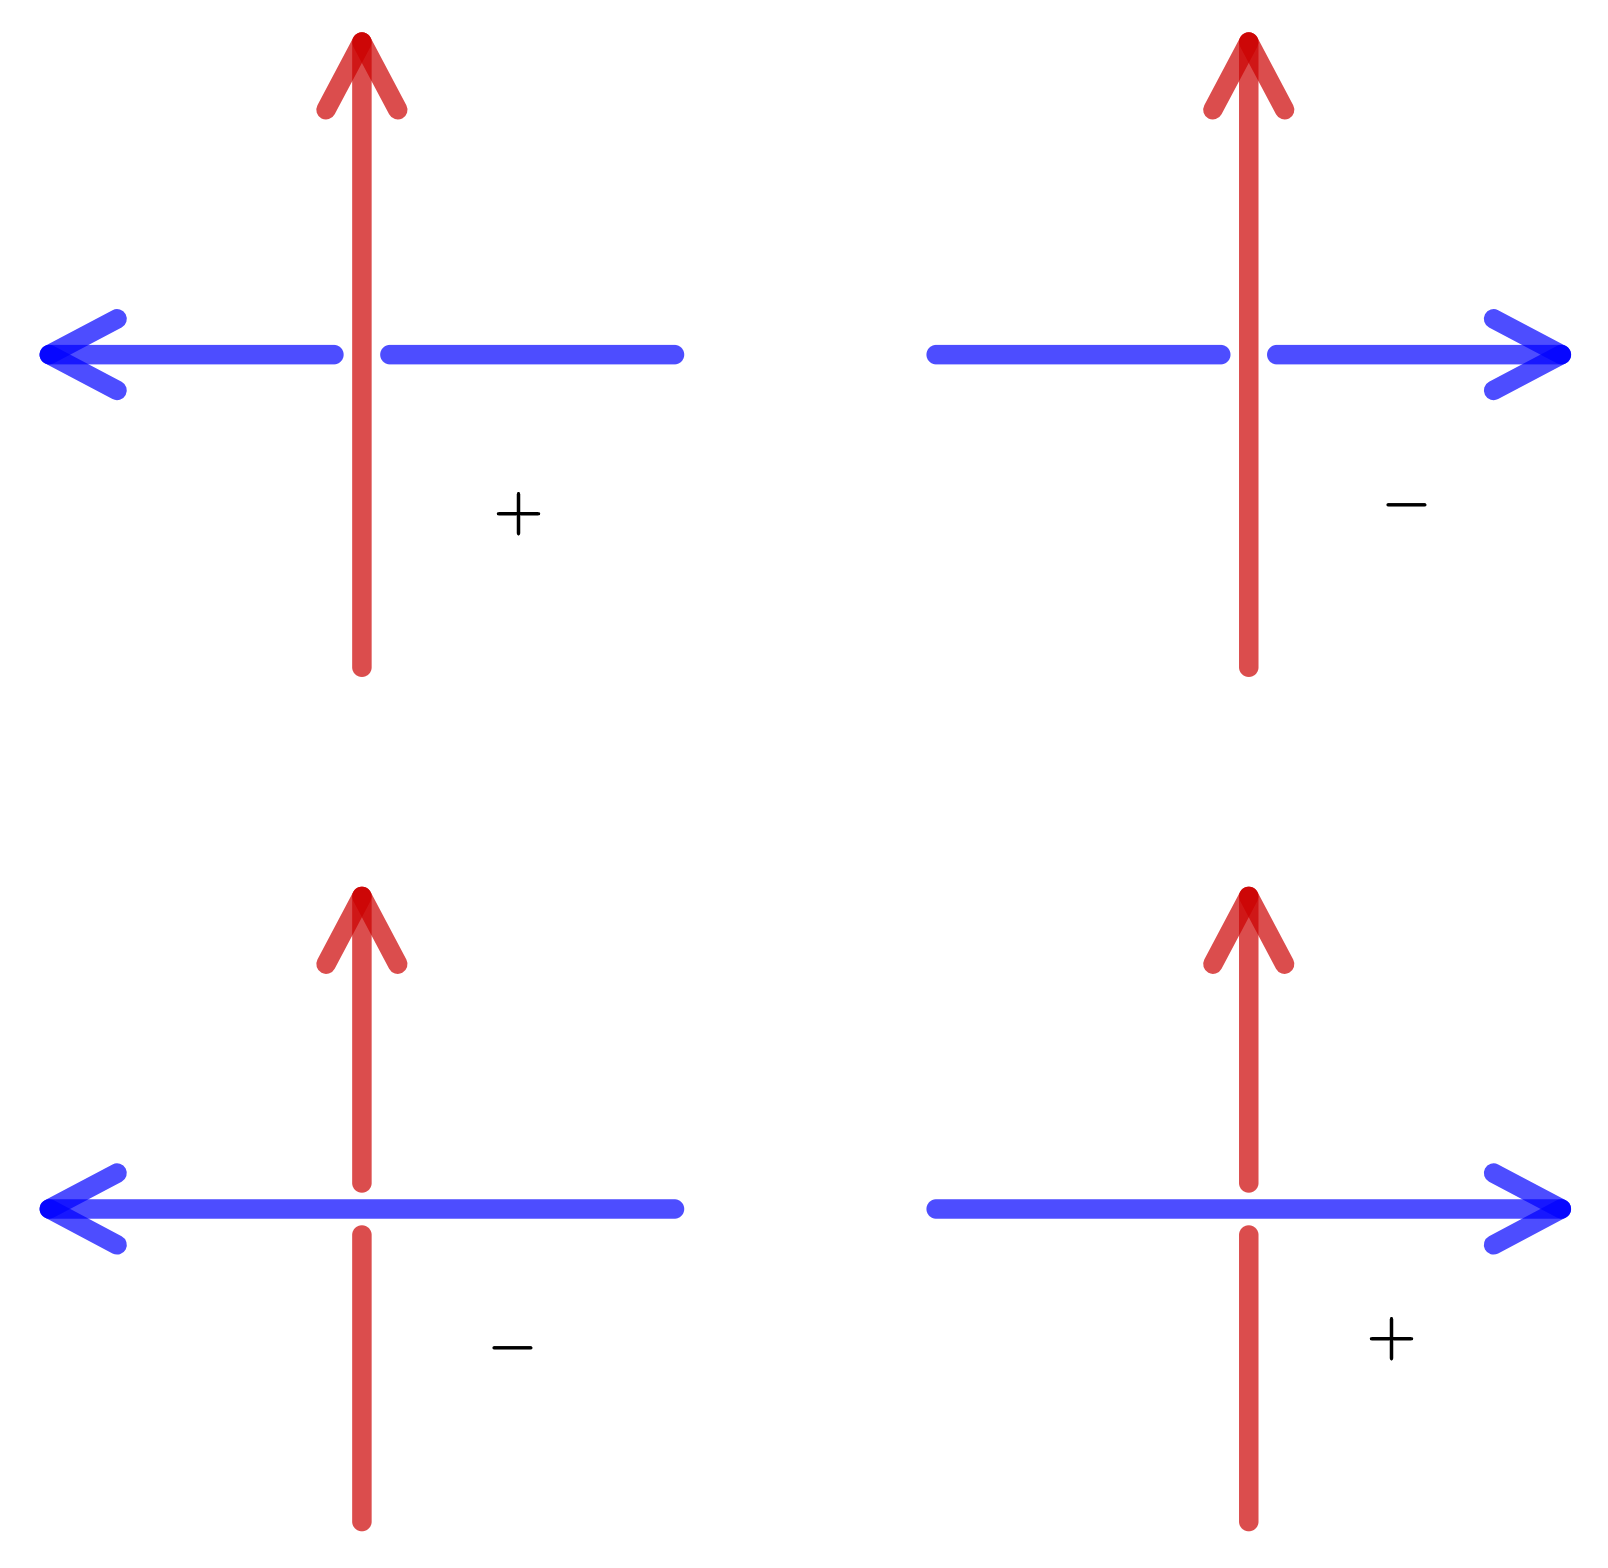
\includegraphics[width= 0.6\linewidth]{h16}
		\caption{\small\textit{\color{duongvaotoanhoc}Hình $16$: Quy tắc tính số liên kết.}}
		\vspace*{-10pt}
	\end{figure}
	Nhiều tính toán cho thấy rằng số liên kết thỏa mãn các tính chất tương tự như {\bf\color{duongvaotoanhoc} ký hiệu Legendre} $\left(\dfrac{p}{q}\right)$ giữa hai số nguyên tố $p, q$ trong lý thuyết thặng dư bậc hai. Ta có thể chứng minh rằng $\text{lk}(K,L) = \text{lk}(L,K)$. Tương ứng, ta có luật tương hỗ bậc hai, nói rằng 
	\begin{align*}
		\left(\dfrac{p}{q}\right) = (-1)^{\tfrac{(p-1)(q-1)}{4}}\left(\dfrac{q}{p}\right).
	\end{align*}
	Bài toán trung tâm của tôpô số học có lẽ là câu hỏi tự nhiên nhất: số nguyên tố nào ứng với nút nào? Đây vẫn là một câu hỏi mở. Nếu một ngày người ta xây dựng được một tương ứng $1-1$ tốt giữa chúng, theo nghĩa mỗi kết quả với số nguyên tố thì ta có kết quả với các nút tương ứng, một số lượng khổng lồ bài toán tôpô học sẽ được giải bằng các kết quả tương tự ở lý thuyết số, và ngược lại.
	
	 Có thể nói, tôpô số học là một trong những ví dụ điển hình nhất về tư tưởng toán học thống nhất, rằng tất cả những đại số, giải tích, hình học, số học... đều chỉ là một.
\end{multicols} 
%	\newpage

%	\setcounter{figure}{0}
%	\thispagestyle{quantoannone}
\pagestyle{quantoan}
\everymath{\color{quantoan}}
\graphicspath{{../quantoan/pic/}}
%\blfootnote{\color{quantoan}\color{quantoan}$^*$Nguồn Math. Intellegencer, Số $41$.}
\begingroup
\AddToShipoutPicture*{\put(0,616){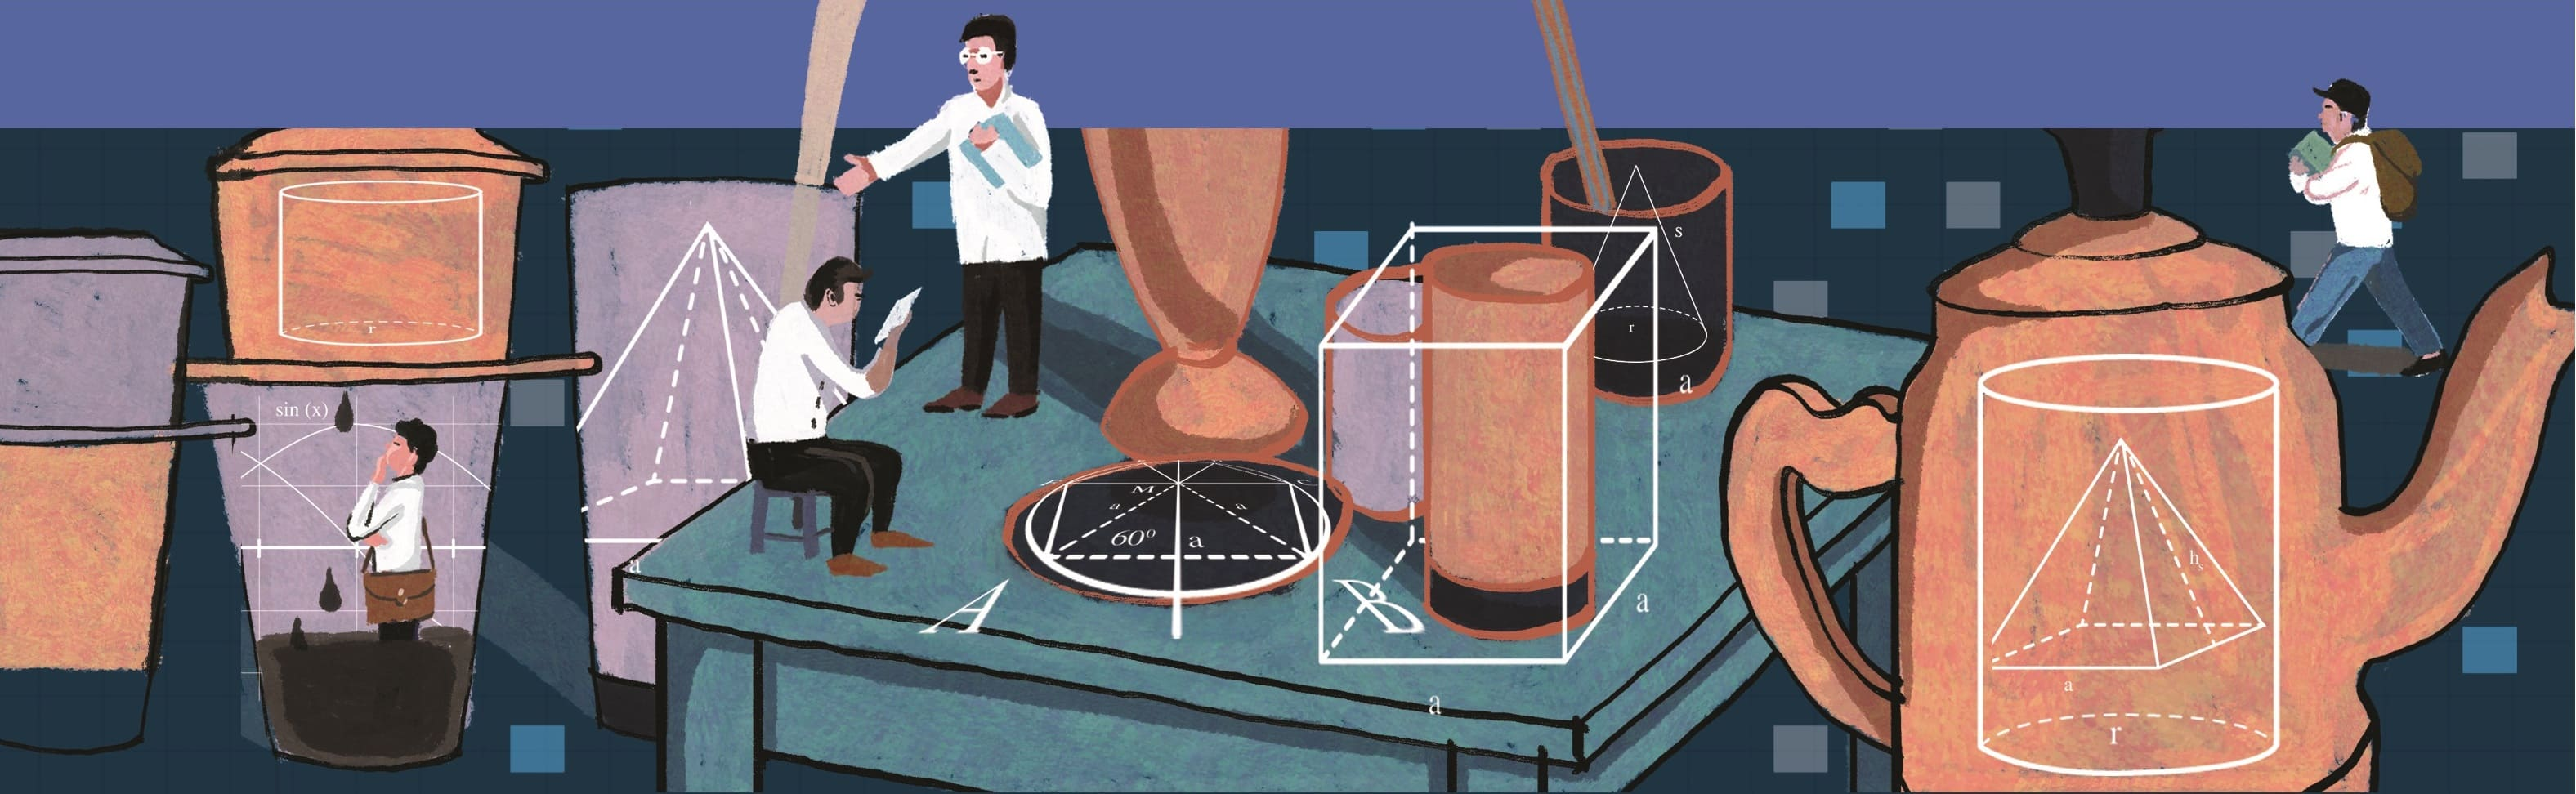
\includegraphics[width=19.3cm]{../bannerquantoan}}}
\AddToShipoutPicture*{\put(120,552){
\includegraphics[scale=1]{../tieude.pdf}}}
\centering
\endgroup
\vspace*{155pt}

\begin{multicols}{2}
	Người ta kể lại rằng nhà toán học Pythagoras đã thiết kế một loại cốc đặc biệt dành cho các học trò của mình (Hình $1$). Ở phần giữa của nó có một lỗ thông xuống đáy được che lại bởi một cấu trúc tạo thành bình thông nhau.
	\begin{figure}[H]
		\vspace*{-5pt}
		\centering
		\captionsetup{labelformat= empty, justification=centering}
		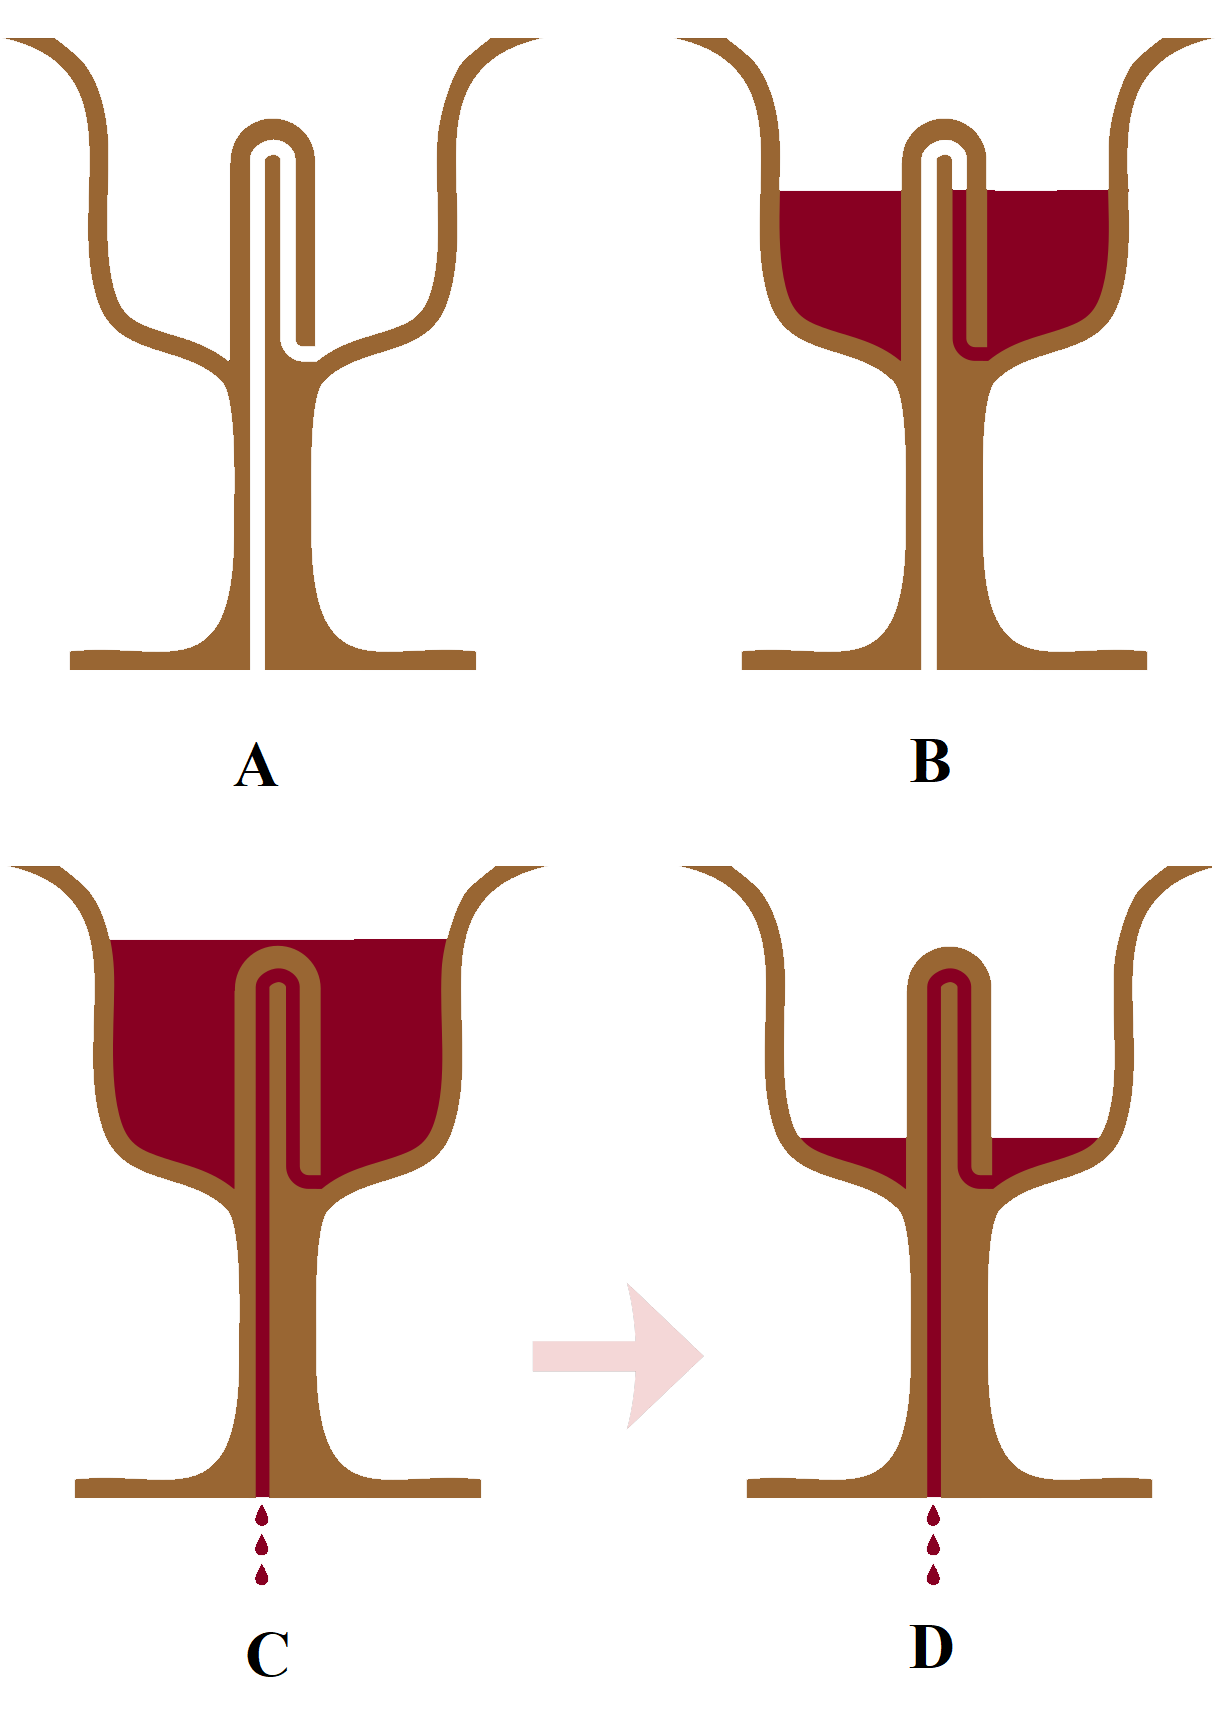
\includegraphics[width= 1\linewidth]{1}
		\caption{\small\textit{\color{quantoan}Hình $1$. Chiếc cốc của Pythagoras. Khi rót đầy chất lỏng vượt ngưỡng, toàn bộ chất lỏng trong cốc sẽ bị chảy ra ngoài}}
		\vspace*{-10pt}
	\end{figure}
	Khi đổ dần rượu vào cốc, mực rượu sẽ dâng lên ở trong cốc cũng như nhánh thông với nó (Hình $1$B). Đến khi mực rượu vượt ngưỡng chứa của nhánh này, nó bắt đầu sẽ bị chảy ra ngoài (Hình $1$C). Nhưng thay vì chỉ rút xuống mức tới hạn trước khi rượu bắt đầu chảy ra, toàn bộ chất lỏng trong cốc lại vẫn tiếp tục tạo thành dòng chảy ra ngoài cho đến khi chảy hết rượu. Những kẻ tham lam sẽ không còn lại gì cả!
	
	Đây là một bài học của Pythagoras cho các học trò của mình về việc phải có chừng mực trong cuộc sống, không được thái quá. Vậy còn bài học về vật lý ở đây là gì? Tại sao rượu lại có thể tiếp tục chảy ngược ra ngoài dù mực rượu trong phần ống cao hơn trong cốc? Những gì ta đã biết về bình thông nhau có bị vi phạm?
	\vskip 0.1cm
	Thực chất của hiện tượng xảy ra trong chiếc cốc của Pythagoras giống với quy trình hoạt động của ống xi phông (Hình $2$). Ống này có dạng ống chữ U ngược với hai đầu đặt ở hai khối chất lỏng khác nhau, một đầu cao hơn đầu còn lại. Chất lỏng trong ống xi phông có thể chảy từ khối chất lỏng cao ngược lên đỉnh chữ U rồi chảy xuống khối chất lỏng ở dưới. Để bắt đầu dòng chảy, người ta cần hút không khí ra khỏi đầu dưới của ống để tạo sự chênh lệch với áp suất khí quyển ở đầu còn lại. Hai mô hình được đưa ra để giải thích hiện tượng này. Trong mô hình thứ nhất, khi chất lỏng chảy vượt qua đỉnh của chữ U ngược, nó tạo ra một vùng áp suất thấp nên áp suất khí quyển từ đầu đường ống sẽ tiếp tục đẩy chất lỏng đi. Mô hình thứ hai dựa trên lực liên kết phân tử, trong đó sự kết dính giữa các khối nước sẽ kéo chúng theo nhau tạo thành dòng chảy. Việc mô hình nào là chính xác vẫn còn là một vấn đề đang được khoa học nghiên cứu.
	\begin{figure}[H]
		\vspace*{-5pt}
		\centering
		\captionsetup{labelformat= empty, justification=centering}
		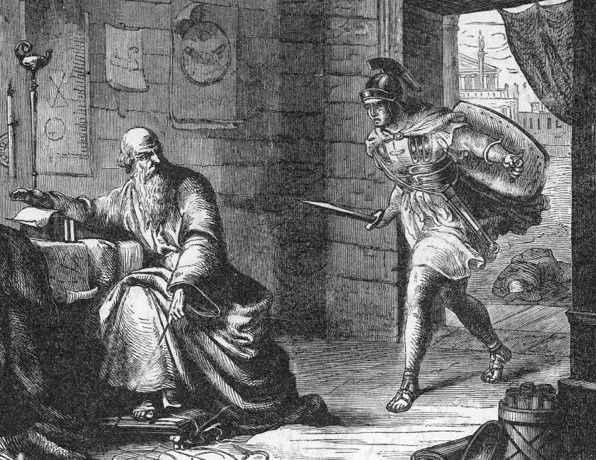
\includegraphics[width= 1\linewidth]{2}
		\caption{\small\textit{\color{quantoan}Hình $2$. Ống xi phông có thể tạo dòng chảy đi lên ngược với chiều của trọng lực nếu hai đầu của chữ U ngược có độ cao khác nhau.}}
		\vspace*{-10pt}
	\end{figure}
	Nếu nhìn lại vào cấu tạo của chiếc cốc Pythagoras, ta có thể thấy ngay một đoạn chữ U ngược tương tự như ống xi phông với một đầu nối với lòng cốc và đầu còn lại nối với chân cốc. Trong thực tế, ống xi phông được sử dụng thường xuyên trong đời sống để tháo nước khỏi các bình chứa, lấy bia ra khỏi thùng bia, rút nước khỏi các mái nhà có diện tích lớn, hay trong khay đựng bột giặt của các máy giặt, ...  Một số nghiên cứu khảo cổ cũng cho thấy ống xi phông đã được sử dụng từ thời Ai Cập cổ đại trong nhiều công việc như dẫn nước thủy lợi hay chế biến đồ uống. 
	\begin{figure}[H]
		\vspace*{-5pt}
		\centering
		\captionsetup{labelformat= empty, justification=centering}
		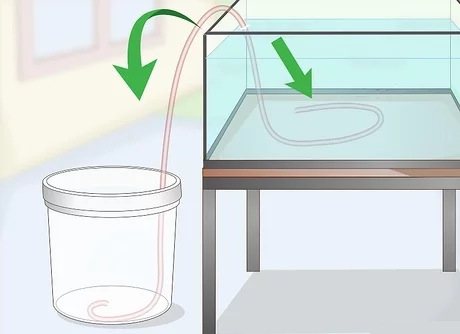
\includegraphics[width= 1\linewidth]{3}
		\caption{\small\textit{\color{quantoan}Hình $3$. Ống xi phông dùng để rút nước khỏi bể chứa.}}
		\vspace*{-10pt}
	\end{figure}
\end{multicols}
%	\newpage
%
	\setcounter{figure}{0}
	\thispagestyle{toancuabinone}
\pagestyle{toancuabi}
\everymath{\color{toancuabi}}
\blfootnote{$^1$\color{toancuabi}Trường Liên cấp Hội nhập Quốc tế iSchool Quảng Trị.}
\graphicspath{{../toancuabi/pic2/}}
\begingroup
\AddToShipoutPicture*{\put(0,616){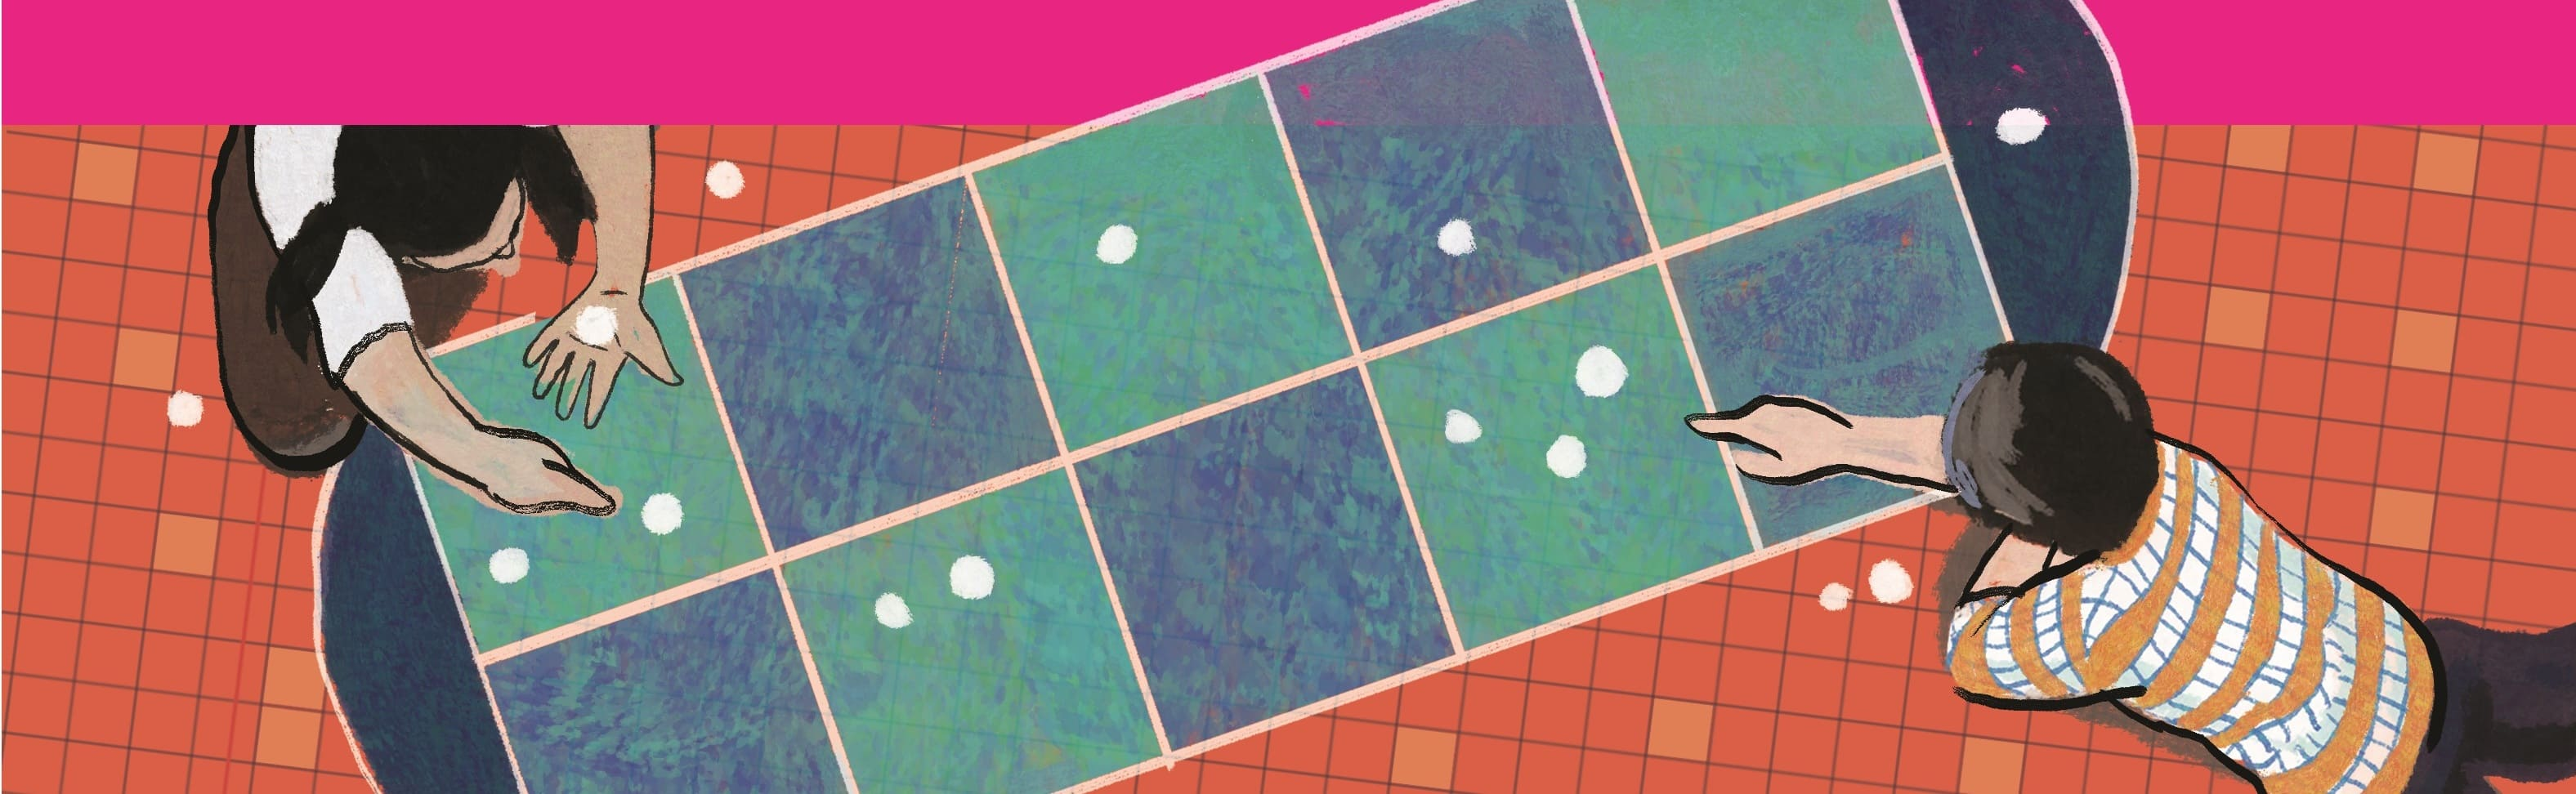
\includegraphics[width=19.3cm]{../bannertoancuabi}}}  
\AddToShipoutPicture*{\put(48,552){
\includegraphics[scale=1]{../tieude10.pdf}}}  
\centering
\endgroup
\vspace*{155pt} 

\begin{multicols}{2}
	Chuồn chuồn tre là sản phẩm độc đáo được các nghệ nhân làng Thạch Xá tạo nên, là món đồ chơi tuổi thơ rất đỗi thân thuộc đối với mỗi người dân trong làng. Lịch sử làng chuồn chuồn tre Thạch Xá với nhiều năm trong nghề đã biến mảnh đất này thành một trong những làng nghề nổi tiếng ở Hà Nội được nhiều du khách biết đến.
	\vskip 0.1cm 
	\begin{center}
		\textit{Chuồn chuồn có cánh thì bay\\
	Có thằng cu Tí thò tay bắt chuồn}
	\end{center}
	\hfill \textit{(Đồng dao, thơ ca dân gian)}
	\begin{figure}[H]
		\vspace*{-5pt}
		\centering
		\captionsetup{labelformat= empty, justification=centering}
		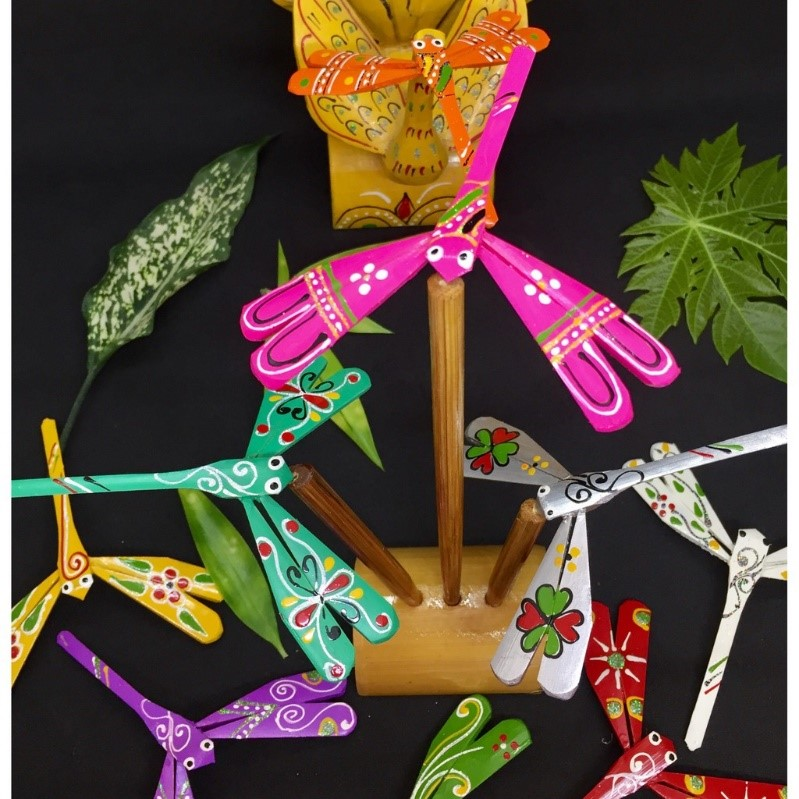
\includegraphics[width= 0.9\linewidth]{10}
		\caption{\small\textit{\color{toancuabi}Ảnh : Internet.}}
		\vspace*{-10pt}
	\end{figure}
	Ngày hôm nay chúng ta sẽ cùng nhau thử sức làm chuồn chuồn tre nhé! Để đơn giản hơn thì chúng ta sẽ thay thế vật liệu để làm chuồn chuồn tre là từ những cây tre thành que kem hoặc giấy.
	\vskip 0.1cm
	\textbf{\color{toancuabi}Cách $\pmb{1}$: Chuồn chuồn que kem thăng bằng}
	\vskip 0.1cm
	\textit{Chuẩn bị nguyên liệu}: 
	\vskip 0.05cm
	-- Các que kem.
	\vskip 0.05cm
	-- Keo, súng bắn keo.
	\vskip 0.05cm
	-- Đũa dùng một lần.
	\vskip 0.05cm
	-- Thước thẳng.
	\vskip 0.05cm
	-- Dao rọc giấy.
	\vskip 0.05cm
	-- Bút chì.
	\vskip 0.05cm
	\textit{Cách làm chuồn chuồn que kem thăng bằng}:
	\vskip 0.1cm
	\textit{Bước} $1$: Sử dụng súng bắn keo dính hai que kem dài $4$ cm lại với nhau.
	\begin{figure}[H]
		\vspace*{-5pt}
		\centering
		\captionsetup{labelformat= empty, justification=centering}
		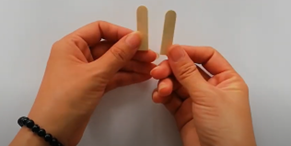
\includegraphics[width=0.7\linewidth]{11}
		
		\vspace*{1pt}
		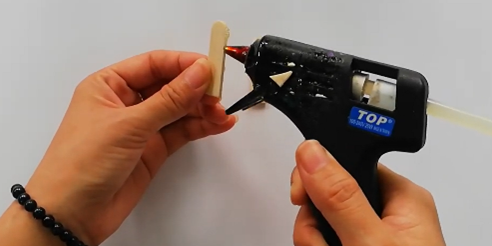
\includegraphics[width=0.7\linewidth]{12}
		
		\vspace*{1pt}
		\hspace*{1pt}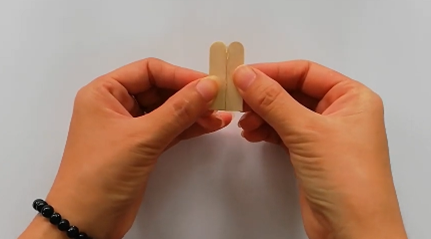
\includegraphics[width=0.7\linewidth]{13}
%		\vspace*{-5pt}
	\end{figure}
	\textit{Bước} $2$: Sử dụng đầu que kem và bút chì để tạo hình phần đầu cho con chuồn chuồn.
	\begin{figure}[H]
		\vspace*{-5pt}
		\centering
		\captionsetup{labelformat= empty, justification=centering}
		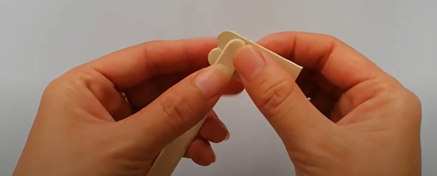
\includegraphics[width=0.7\linewidth]{14}
		
		\vspace*{1pt}
		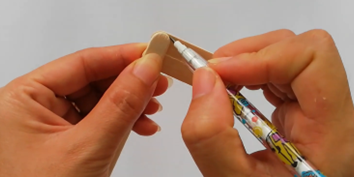
\includegraphics[width=0.7\linewidth]{15}
		
		\vspace*{1pt}
		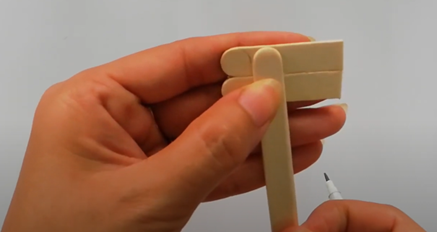
\includegraphics[width=0.7\linewidth]{16}
		
		\vspace*{1pt}
		\hspace*{1pt}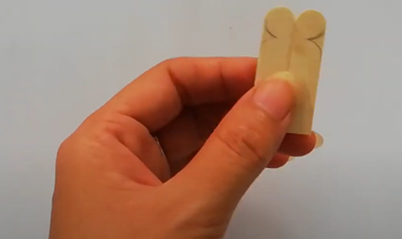
\includegraphics[width=0.7\linewidth]{17}
		\vspace*{-5pt}
	\end{figure}
	\textit{Bước} $3$: Sử dụng dao rọc giấy cắt đi phần khuyết.
	\begin{figure}[H]
		\vspace*{-5pt}
		\centering
		\captionsetup{labelformat= empty, justification=centering}
		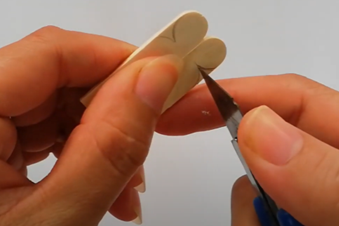
\includegraphics[width=0.7\linewidth]{18}
		
		\vspace*{1pt}
		\hspace*{1pt}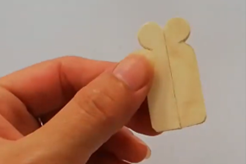
\includegraphics[width=0.7\linewidth]{19}
		\vspace*{-10pt}
	\end{figure}
	\textit{Bước} $4$: Lấy que kem nguyên vẹn rồi cắt chéo đi một nửa (như hình minh họa), sau đó dùng súng bắn keo dán vào que kem dài 10cm để làm cánh chuồn chuồn. (Lưu ý là chuồn chuồn có cánh dài, cánh ngắn).
	\begin{figure}[H]
		\vspace*{5pt}
		\centering
		\captionsetup{labelformat= empty, justification=centering}
		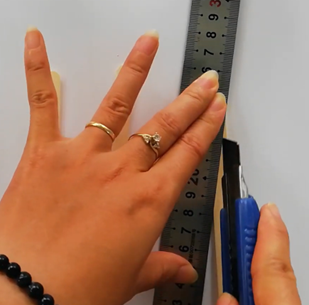
\includegraphics[height=0.35\linewidth]{50}
		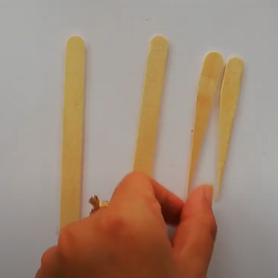
\includegraphics[height=0.35\linewidth]{51}
		
		\vspace*{1pt}
		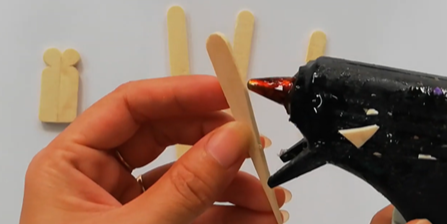
\includegraphics[width=0.7\linewidth]{52}
		
		\vspace*{1pt}
		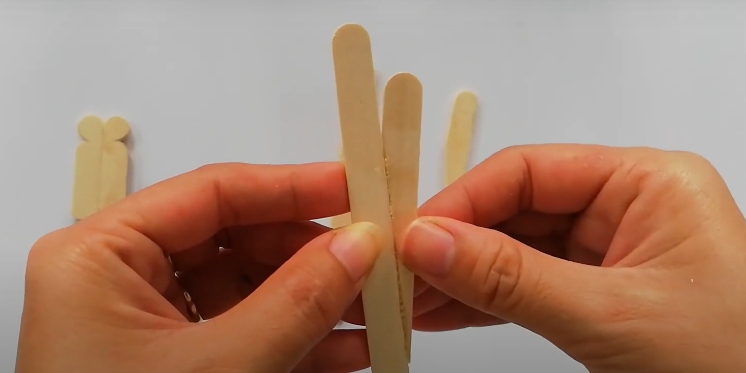
\includegraphics[width=0.7\linewidth]{53}
		
		\vspace*{1pt}
		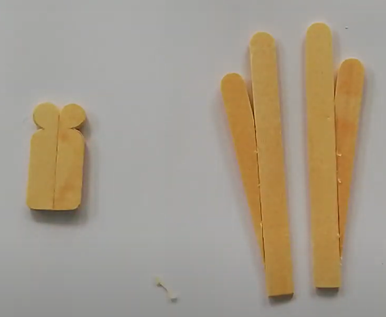
\includegraphics[width=0.7\linewidth]{54}
		\vspace*{-10pt}
	\end{figure}
	\textit{Bước} $5$: Sử dụng súng bắn keo để dán que kem dài $10$ cm vào phần đầu của con chuồn chuồn.
	\begin{figure}[H]
		\vspace*{-5pt}
		\centering
		\captionsetup{labelformat= empty, justification=centering}
		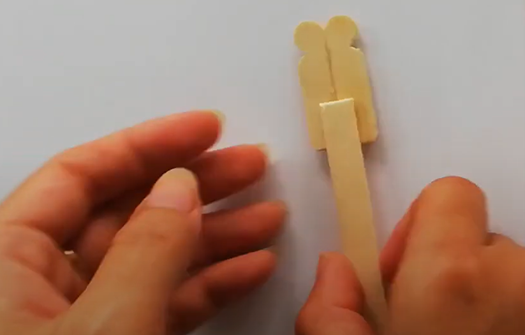
\includegraphics[width=0.7\linewidth]{55}
		\vspace*{-10pt}
	\end{figure}
	\textit{Bước} $6$: Tiếp tục sử dụng súng bắn keo dán hai cánh chuồn chuồn vào thân.
	\begin{figure}[H]
		\vspace*{-5pt}
		\centering
		\captionsetup{labelformat= empty, justification=centering}
		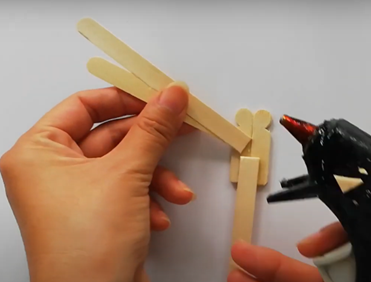
\includegraphics[height=0.36\linewidth]{56}
		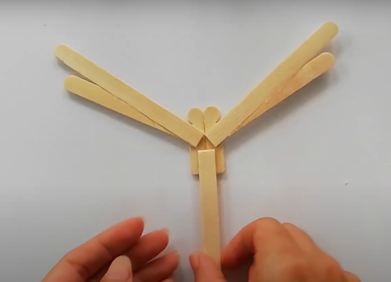
\includegraphics[height=0.36\linewidth]{57}
		\vspace*{-10pt}
	\end{figure}
	\textit{Bước} $7$: Sử dụng súng bắn keo để dán que tre tròn (hoặc đũa dùng một lần) vào chính giữa que kem nguyên vẹn để làm giá đỡ chuồn chuồn.
	\begin{figure}[H]
		\vspace*{5pt}
		\centering
		\captionsetup{labelformat= empty, justification=centering}
		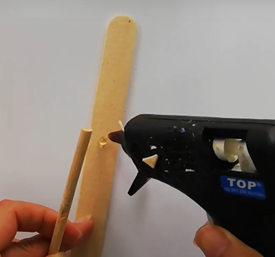
\includegraphics[height=0.34\linewidth]{58}
		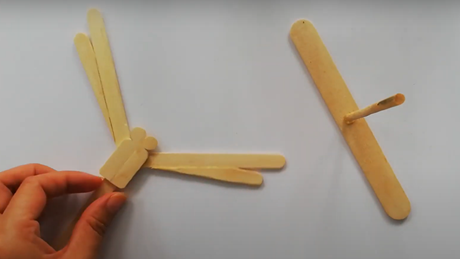
\includegraphics[height=0.34\linewidth]{59}
		\vspace*{-10pt}
	\end{figure}
	Cuối cùng, các em chỉ cần đặt chuồn chuồn lên giá đỡ hoặc lên ngón tay của mình là chuồn chuồn có thể tự thăng bằng được rồi.
	\begin{figure}[H]
		\vspace*{-5pt}
		\centering
		\captionsetup{labelformat= empty, justification=centering}
		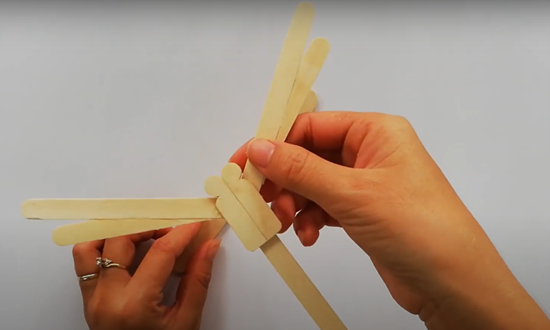
\includegraphics[height=0.35\linewidth]{60}
		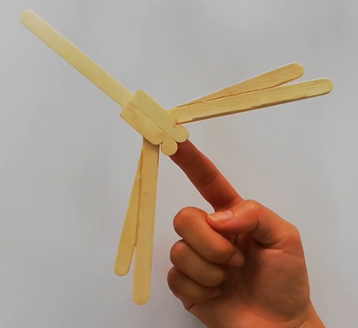
\includegraphics[height=0.35\linewidth]{61}
		\vspace*{-10pt}
	\end{figure}
	\textbf{\color{toancuabi}Cách $\pmb{2}$: Chuồn chuồn giấy thăng bằng}
	\vskip 0.1cm
	\textit{Chuẩn bị nguyên liệu}:
	\vskip 0.1cm
	-- Giấy bìa màu.
	\vskip 0.1cm
	-- Nắp nhựa (tái sử dụng từ chai nhựa bỏ đi).
	\vskip 0.1cm
	-- Đũa dùng một lần.
	\vskip 0.1cm
	-- Bút chì.
	\vskip 0.1cm
	-- Kéo.
	\vskip 0.1cm
	-- Hồ dán.
	\vskip 0.1cm
	-- Keo, súng bắn keo.
	\vskip 0.1cm
	\textit{Cách làm chuồn chuồn giấy thăng bằng}:
	\vskip 0.1cm
	\textit{Bước} $1$: Gấp đôi giấy bìa màu hình chữ nhật (có chiều dài $13$ cm và chiều rộng $4$ cm).
	\begin{figure}[H]
		\vspace*{-5pt}
		\centering
		\captionsetup{labelformat= empty, justification=centering}
		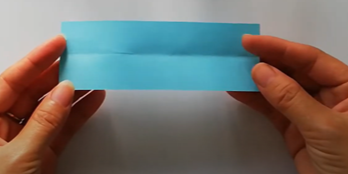
\includegraphics[width=0.7\linewidth]{62}
		
		\vspace*{1pt}
		\hspace*{1pt}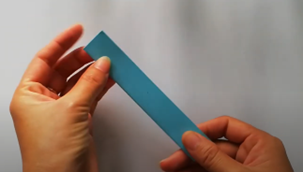
\includegraphics[width=0.7\linewidth]{63}
		\vspace*{-10pt}
	\end{figure}
	\textit{Bước} $2$: Sử dụng bút chì vẽ hình dạng con chuồn chuồn lên tờ giấy màu, sau đó dùng kéo cắt ra.
	\begin{figure}[H]
		\vspace*{5pt}
		\centering
		\captionsetup{labelformat= empty, justification=centering}
		\includegraphics[width=0.7\linewidth]{64}
		
		\vspace*{1pt}
		\includegraphics[width=0.7\linewidth]{65}
		
		\vspace*{1pt}
		\hspace*{1pt}\includegraphics[width=0.7\linewidth]{66}
		\vspace*{-10pt}
	\end{figure}
	\textit{Bước} $3$: Gấp đôi giấy bìa màu hình chữ nhật (có chiều dài $11$ cm và chiều rộng $5$ cm).
	\begin{figure}[H]
		\vspace*{-5pt}
		\centering
		\captionsetup{labelformat= empty, justification=centering}
		\includegraphics[width=0.7\linewidth]{67}
		
		\vspace*{1pt}
		\includegraphics[width=0.7\linewidth]{68}
		\vspace*{-10pt}
	\end{figure}
	\textit{Bước} $4$: Sử dụng bút chì vẽ hình dạng cánh chuồn chuồn lên tờ giấy màu, sau đó dùng kéo cắt ra.
	\begin{figure}[H]
		\vspace*{-5pt}
		\centering
		\captionsetup{labelformat= empty, justification=centering}
		\includegraphics[height=0.31\linewidth]{69}
		\includegraphics[height=0.31\linewidth]{70}
		
		\vspace*{1pt}
		\includegraphics[width=0.7\linewidth]{71}
		\vspace*{-10pt}
	\end{figure}
	\textit{Bước} $5$: Làm tương tự với giấy bìa màu hình chữ nhật (có chiều dài $9$ cm và chiều rộng $4{,}5$~cm) để tạo ra hai cánh nhỏ hơn cho chuồn chuồn.
	\begin{figure}[H]
		\vspace*{-5pt}
		\centering
		\captionsetup{labelformat= empty, justification=centering}
		\includegraphics[width=0.7\linewidth]{72}
		\vspace*{-10pt}
	\end{figure}
	\textit{Bước} $6$: Sử dụng hồ dán để dán cánh chuồn chuồn vào thân chuồn chuồn.
	\begin{figure}[H]
		\vspace*{-5pt}
		\centering
		\captionsetup{labelformat= empty, justification=centering}
		\includegraphics[width=0.7\linewidth]{73}
		\vspace*{-10pt}
	\end{figure}
	\textit{Bước} $7$: Sử dụng súng bắn keo để dán que tre tròn (hoặc đũa dùng một lần) vào chính giữa nắp nhựa để làm giá đỡ chuồn chuồn.
	\begin{figure}[H]
		\vspace*{-5pt}
		\centering
		\captionsetup{labelformat= empty, justification=centering}
		\includegraphics[width=0.7\linewidth]{74}
		\vspace*{-10pt}
	\end{figure}
	Cuối cùng, đặt chuồn chuồn giấy lên giá đỡ hoặc lên ngón tay của mình là chuồn chuồn có thể tự thăng bằng được rồi.
	\begin{figure}[H]
		\vspace*{-5pt}
		\centering
		\captionsetup{labelformat= empty, justification=centering}
		\includegraphics[width=0.7\linewidth]{75}
		\vspace*{-10pt}
	\end{figure}
\end{multicols}

%\begin{multicols}{2}
%	Thám tử Xuân Phong cùng thanh tra Lê Kính tham gia một buổi giới thiệu sản phẩm của hai công ty là Tae Yeon và Tea Yon tại triển lãm Điện tử Expo -- New Vision của khu vực. Công ty  Tae Yeon có uy tín từ lâu đời, với những sản phẩm tinh tế có chất lượng tốt nổi tiếng,  các nhân viên của công ty luôn nói thật. Còn công ty Tea Yon chuyên sản xuất đồ rẻ, kém chất lượng, bắt chước kiểu dáng của công ty Tae Yeon nên Ban giám đốc dặn các nhân viên của mình chỉ được nói dối trong buổi triển lãm. 
%	\vskip 0.1cm
%	Vừa đặt chân tới khu vực triển lãm được trang hoàng lộng lẫy, Xuân Phong gặp ngay $5$ đại diện  của hai công ty này đứng tại cổng ra vào và tươi cười niềm nở tiếp đón. Xuân Phong tiến tới họ và hỏi cả $5$ người cùng một câu hỏi ``Có bao nhiêu người đến từ công ty Tae Yeon trong số các bạn?" 
%	\vskip 0.1cm
%	Người thứ nhất trả lời ``Không có ai cả". Hai người tiếp theo đều trả lời ``Có đúng một người". 
%	\vskip 0.1cm
%	Vậy hai người còn lại sẽ trả lời câu hỏi của thám tử Xuân Phong như thế nào nhỉ? Em có thể suy đoán ra câu trả lời của họ và giải thích lập luận được không?
%	\begin{figure}[H]
	%		\centering
	%		\vspace*{-5pt}
	%		\captionsetup{labelformat= empty, justification=centering}
	%		\includegraphics[width=1\linewidth]{xuanphong}
	%		\vspace*{-5pt}
	%	\end{figure}
%\end{multicols}
%\vspace*{-10pt}
%{\color{toancuabi}\rule{1\linewidth}{0.1pt}}
%\begingroup
%\AddToShipoutPicture*{\put(115,190){\includegraphics[scale=1]{../tieude11.pdf}}} 
%\centering
%\endgroup
%\vspace*{50pt}
%
%\begin{multicols}{2}
%	$\pmb{1.}$	Trong một cuộc thi thể thao, ban tổ chức chọn ra một số bạn học sinh ở lớp $5A$ và một số bạn ở lớp $5B$ thi đấu trực tiếp. Mỗi bạn ở lớp $5A$ được chọn ra sẽ thi đấu duy nhất một trận với một bạn ở lớp $5B$, và ngược lại, mỗi bạn ở lớp $5B$ được chọn ra chỉ đấu đúng một trận với một bạn ở lớp $5A$.
%	\begin{figure}[H]
	%		\centering
	%		\vspace*{-5pt}
	%		\captionsetup{labelformat= empty, justification=centering}
	%		\includegraphics[width=1\linewidth]{Pi5_bai1}
	%		\vspace*{-15pt}
	%	\end{figure}
%	Biết rằng số học sinh lớp $5A$ được chọn thi đấu chiếm $2/3$ tổng số học sinh toàn lớp $5A$, còn số học sinh lớp $5B$ được chọn thi đấu chiếm $3/5$ tổng số học sinh toàn lớp $5B$. Tổng số học sinh của cả hai lớp là $57$ bạn. Hỏi có bao nhiêu học sinh của hai lớp đã tham gia các trận thi đấu trực tiếp?
%	
%	$\pmb{2.}$ Công ty vận tải được thông báo ngắn gọn là có một số kiện hàng có tổng khối lượng là $10$ tấn cần được vận chuyển, hơn nữa mỗi kiện hàng nặng không quá $1$ tấn. Hỏi công ty  cần điều động ít nhất bao nhiêu xe tải có trọng tải là $3$ tấn mỗi xe để luôn chắc chắn chở được hết được số hàng hoá đó?
%	\begin{figure}[H]
	%		\centering
	%		\vspace*{-10pt}
	%		\captionsetup{labelformat= empty, justification=centering}
	%		\includegraphics[width=0.8\linewidth]{Pi5_bai2}
	%		\vspace*{-15pt}
	%	\end{figure}
%	$\pmb{3.}$ Sau khi được sạc đầy pin, điện thoại di động của bạn An dùng đúng $6$ tiếng ở chế độ trò chuyện hoặc đúng $210$ tiếng ở chế độ chờ. Khi bạn An lên tàu hoả để đi du lịch, pin của bạn được sạc đầy $100\%$, và trên tàu không có ổ cắm sạc nên khi xuống ga, pin của bạn cũng vừa hết sạch. Biết rằng An đã nói chuyện với bạn bè đúng một nửa thời gian khi ngồi trên tàu, còn nửa thời gian còn lại đặt điện thoại ở chế độ chờ. Hỏi thời gian An đi trên tàu hoả là bao nhiêu lâu?
%	\begin{figure}[H]
	%		\centering
	%		\vspace*{-5pt}
	%		\captionsetup{labelformat= empty, justification=centering}
	%		\includegraphics[width=0.85\linewidth]{Pi5_bai3}
	%		\vspace*{-10pt}
	%	\end{figure}
%	$\pmb{4.}$ Một nhóm học sinh đi bộ từ điểm hẹn tới bến xe buýt để kịp đón chuyến xe vào lúc $8$ giờ. Cũng vào thời điểm này, từ điểm tham quan, một chiếc xe buýt cũng xuất phát để tới kịp bến xe đón nhóm học sinh đó. Tuy  nhiên nhóm học sinh tới bến xe buýt khá sớm, vào lúc $6$ giờ $10$ phút, nên họ quyết định đi bộ tiếp tới điểm tham quan. Trên đường, các bạn đã gặp được xe buýt và lên xe đi tiếp.  Cuối cùng cả nhóm đến được điểm tham quan sớm hơn $20$ phút so với thời gian ấn định. Biết rằng vận tốc của xe buýt là $60$ km/h và vận tốc đi bộ của các em học sinh luôn không đổi. Hãy tìm vận tốc đi bộ của nhóm học sinh trước khi gặp xe buýt.
%	\begin{figure}[H]
	%		\centering
	%		\vspace*{-10pt}
	%		\captionsetup{labelformat= empty, justification=centering}
	%		\includegraphics[width=0.85\linewidth]{Pi5_bai4}
	%		\vspace*{-10pt}
	%	\end{figure}
%	$\pmb{5.}$ 	Có $100$ chiếc xe ô tô đỗ liền nhau thành một hàng dọc bên lề đường, trong đó có $70$ chiếc xe hiệu Mercedes, còn lại là những xe nhãn hiệu khác. Trong các xe nhãn hiệu Mercedes có $30$ chiếc màu đỏ, $20$ chiếc màu vàng và $20$ chiếc màu hồng. Biết rằng không có hai xe Mercedes nào khác màu lại đỗ cạnh nhau. Em hãy chỉ ra rằng luôn tìm ra $3$ chiếc xe Mercedes cùng màu đỗ liên tiếp nhau.
%	\begin{figure}[H]
	%		\centering
	%		\vspace*{-5pt}
	%		\captionsetup{labelformat= empty, justification=centering}
	%		\includegraphics[width=0.85\linewidth]{Pi5_bai5}
	%		\vspace*{-10pt}
	%	\end{figure}
%	$\pmb{6.}$ Một lớp học có $20$ em học sinh. Cô giáo chủ nhiệm của lớp tổ chức một số buổi tham quan vào mỗi ngày cuối tuần trong suốt năm học, mỗi buổi tham quan có ít nhất $4$ em học sinh tham gia. Em hãy chứng minh rằng có một buổi tham quan mà mỗi em học sinh tham gia buổi đó đều tham gia ít nhất $1/17$ tổng số tất cả các buổi tham quan của cả năm học.
%	\begin{figure}[H]
	%		\centering
	%		\vspace*{-15pt}
	%		\captionsetup{labelformat= empty, justification=centering}
	%		\includegraphics[width=0.8\linewidth]{Pi5_bai6}
	%		%		\vspace*{-5pt}
	%	\end{figure}
%\end{multicols}
%\newpage
%\begingroup
%\AddToShipoutPicture*{\put(110,645){\includegraphics[scale=1]{../tieude2.pdf}}} 
%\centering
%\endgroup
%\vspace*{55pt}
%
%\begin{multicols}{2}
%	$\pmb{1.}$ Một bác nông dân chở một xe ô tô quất cảnh ra chợ Tết để bán. Sau khi bán hết cây quất cuối cùng với giá $230$ nghìn đồng, bác tính nhẩm lại thấy mình đã bán số cây quất với giá trung bình là $245$ nghìn đồng/cây. Nhưng ngay lúc ấy người mua cây quất cuối quay trở lại và chỉ cho bác thấy cành quất bị rụng quá nhiều lá, nên ông ta chỉ đồng ý mua với giá $158$ nghìn đồng. 
%	Bác chấp thuận và bán cây quất đó. Khi nhẩm tính lại, bác nông dân thấy giá trung bình của xe quất bây giờ là $242$ nghìn đồng/cây. Hỏi bác đã bán được bao nhiêu cây quất?
%	\begin{figure}[H]
	%		\centering
	%		\vspace*{-10pt}
	%		\captionsetup{labelformat= empty, justification=centering}
	%		\includegraphics[width=0.7\linewidth]{Pi1_2_Bai1}
	%		\vspace*{-15pt}
	%	\end{figure}
%	\textit{Lời giải.} Gọi số cây quất là $n$, và tổng số tiền bán được của toàn bộ số quất, trừ cây cuối cùng, là $q$ (nghìn đồng). Khi đó $q+230 = 245n$ và $q+ 158 = 242n$. Trừ hai đẳng thức này ta có $72 = 3n$. Suy ra bác nông dân đã bán được $24$ cây quất.
%	\vskip 0.1cm
%	$\pmb{2.}$ Chuyện kể rằng có một người khi gặp nhà triết học và toán học Hy Lạp Pythagoras đã hỏi ông: ``Bây giờ là mấy giờ?" Pythagoras đã trả lời ``Cho đến hết ngày, còn lại hai lần của hai phần năm khoảng thời gian đã trôi qua từ lúc bắt đầu ngày". Nghe vậy, người đó chịu không thể nghĩ ra ngay được lúc họ gặp nhau là mấy giờ. Em có thể giúp trả lời lúc đó là mấy giờ được không?
%	\vskip 0.1cm
%	\textit{Lời giải.} 	Gọi $x$ là thời gian (tính theo giờ) đã trôi qua từ lúc bắt đầu ngày. Khi đó ta có hệ thức sau theo câu trả lời của Pythagoras: $24 - x = 4/5 x$. Suy ra $x = 40/3$ (giờ), có nghĩa là $13$ giờ $20$ phút. Vậy người đó đã gặp Pythagoras lúc $13$ giờ $20$ phút.
%	\begin{figure}[H]
	%		\centering
	%		\vspace*{-10pt}
	%		\captionsetup{labelformat= empty, justification=centering}
	%		\includegraphics[width=0.6\linewidth]{Pi1_2_Bai2}
	%		\vspace*{-10pt}
	%	\end{figure}
%	$\pmb{3.}$ Một tháng trước bà Hoa ra chợ mua một cân khoai tây, một cân thịt và một chục trứng. Chủ nhật vừa rồi, khoai tây tăng lên gấp $3$, thịt gấp $4$ lần còn trứng đắt gấp $5$ lần, nên bà Hoa phải trả $600$ nghìn cho từng ấy món hàng như lần thứ nhất. Hôm nay thì khoai lại đắt gấp $6$ lần so với tháng trước, thịt đắt gấp $5$ lần còn trứng chỉ đắt gấp $4$ lần nên bà Hoa lại phải trả $660$ nghìn với cùng một lượng hàng. Hỏi bà Hoa đã trả bao nhiêu tiền cho lần mua thứ nhất?
%	\begin{figure}[H]
	%		\centering
	%		\vspace*{-10pt}
	%		\captionsetup{labelformat= empty, justification=centering}
	%		\includegraphics[width=0.6\linewidth]{Pi1_2_Bai3}
	%		\vspace*{-10pt}
	%	\end{figure}
%	\textit{Lời giải.} 	Giả sử vào tháng trước trong lần mua đầu tiên giá một cân khoai tây là $a$ (nghìn đồng), giá một cân thịt là $b$ (nghìn đồng) và giá một chục trứng là $c$ (nghìn đồng). Khi đó trong lần mua thứ nhất bà Hoa đã trả $a + b + c$ (nghìn), trong lần mua thứ hai là $3a+4b+5c = 600$ và trong lần mua thứ ba là $6a + 5b+ 4c = 660$. Cộng hai đẳng thức cuối này, ta có $9(a+b+c)= 1260$. Suy ra $a+b+c = 140$. Vậy vào tháng trước bà Hoa chỉ phải trả có $140$ nghìn đồng.
%	\vskip 0.1cm
%	$\pmb{4.}$ Trong một buổi dạ hội nọ mỗi quý ông đã hân hạnh khiêu vũ với ba quý bà, còn mỗi quý bà cũng đã khiêu vũ với ba quý ông. Em hãy chỉ ra rằng số quý ông và số quý bà tham gia dạ hội là bằng nhau.
%	\begin{figure}[H]
	%		\centering
	%		\vspace*{-5pt}
	%		\captionsetup{labelformat= empty, justification=centering}
	%		\includegraphics[width=0.75\linewidth]{Pi1_2_Bai4}
	%		\vspace*{-10pt}
	%	\end{figure}
%	\textit{Lời giải.} Ta sẽ tính tổng tất cả các cặp đã khiêu vũ với nhau. Một mặt, tổng này sẽ bằng $3$ lần số các quý ông, mặt khác nó lại bằng $3$ lần số các quý bà. Vì thế số các quý ông bằng số các quý bà.
%	\vskip 0.1cm
%	$\pmb{5.}$ 	Sau khi kết thúc một giải thi cờ vua, ban tổ chức nhận thấy mỗi kỳ thủ tham gia đã có số trận thắng khi chơi bằng quân trắng bằng đúng tổng số trận thắng của toàn bộ các kỳ thủ còn lại khi chơi quân đen. Em hãy chỉ ra rằng tất cả các kỳ thủ tham gia thi đấu đã có số trận thắng là như nhau.
%	\begin{figure}[H]
	%		\centering
	%		\vspace*{-5pt}
	%		\captionsetup{labelformat= empty, justification=centering}
	%		\includegraphics[width=0.6\linewidth]{Pi1_2_Bai5}
	%		\vspace*{-10pt}
	%	\end{figure}
%	\textit{Lời giải.} Các em có thể nhận thấy số trận thắng của mỗi kỳ thủ tham gia giải bằng đúng tổng số trận thắng của tất cả các kỳ thủ (kể cả chính kỳ thủ đó) khi chơi bằng quân đen. Vì thế mọi kỳ thủ tham gia đã có số trận thắng bằng nhau.
%	\vskip 0.1cm
%	$\pmb{6.}$ Vào một ngày Chủ nhật nọ, Vinh và người em trai nhỏ tuổi hơn là Minh  đạp hai chiếc xe tới hiệu sách trung tâm cách nhà vài cây số. Tại đó mỗi người chọn mua một cuốn sách quý mà nhóm bạn bè cũ đang bàn luận khen ngợi thường xuyên mấy năm nay trên Facebook. Mỗi người đều lấy tổng tất cả các chữ số của tất cả các trang sách mình đã mua và nhận thấy rằng số đó bẳng năm sinh của mình. Vậy ai  trong số hai anh em Vinh và Minh  đang đi học lớp  bồi dưỡng Toán cho học sinh phổ thông nhỉ?
%	\begin{figure}[H]
	%		\centering
	%		\vspace*{-5pt}
	%		\captionsetup{labelformat= empty, justification=centering}
	%		\includegraphics[width=0.8\linewidth]{Pi1_2_Bai6}
	%		\vspace*{-10pt}
	%	\end{figure}
%	\textit{Lời giải.} 	Trước tiên ta tính tổng chữ số của tất cả các số từ $1$ tới $99$. Nhận thấy rằng mỗi chữ số, trừ chữ số $0$ đều xuất hiện $10$ lần ở hàng chục, và cũng $10$ lần ở hàng đơn vị, nghĩa là $20$ lần tổng cộng. Do $1+2+ \cdots+9=45$, nên tổng này bằng  $900$. Tổng các chữ số của các số từ $100$ tới $199$ sẽ lớn hơn tổng trước là $100$. Vì thế tổng các chữ số của các số từ $1$ tới $199$ bằng $1900$. Vì vậy ta xét một vài trường hợp sau.
%	\begin{table}[H]
	%		\centering
	%		\vspace*{-5pt}
	%		\captionsetup{labelformat= empty, justification=centering}
	%		\renewcommand{\arraystretch}{1.05}
	%		\begin{tabular}{|l|l|}
		%			\hline
		%			\textbf{\color{toancuabi}Số trang sách}&	\textbf{\color{toancuabi}Tổng các chữ số}\\
		%			\hline
		%			$200$&	$1900+2 =1902$\\
		%			\hline
		%			$202$&	$1902+3+4=1909$\\
		%			\hline
		%			$204$&	$1909+5+6=1920$\\
		%			\hline
		%			$206$&	$1920+7+8=1935$\\
		%			\hline
		%			$208$&	$1935+9+10=1954$\\
		%			\hline
		%			$210$&	$1954+11+3=1968$\\
		%			\hline
		%			$212$&	$1968+4+5=1977$\\
		%			\hline
		%			$214$&	$1977+6+7=1990$\\
		%			\hline
		%			$216$&	$1990+8+9=2007$\\
		%			\hline
		%			$217$&	$2007+10=2017$\\
		%			\hline
		%			$218$&	$2017+11=2028$\\
		%			\hline
		%		\end{tabular}
	%		\vspace*{-5pt}
	%	\end{table}
%	Các em thấy ngay chỉ có người sinh năm $2007$ trong số hai anh em mới có thể là học sinh phổ thông. Người đó cũng không thể là anh, vì nếu vậy người em trai sinh năm $2017$ đến giờ mới có $5$ tuổi không thể tự đi xe đạp vài cây số để mua sách dày hơn hai trăm trang và về nhà tự làm tính cộng hết từng đó chữ số, hơn nữa lại có nhóm bạn bè cũ trên Facebook bàn luận về cuốn sách tới mấy năm rồi. Vì vậy các em kết luận được người sinh năm $2007$ là em và có tên là Minh.
%\end{multicols}
%\newpage
%\begingroup
%\thispagestyle{toancuabinone}
%%\blfootnote{$^1$\color{toancuabi}Ottawa, Canada.}
%\AddToShipoutPicture*{\put(60,733){\includegraphics[width=17.2cm]{../mathc.pdf}}}
%%\AddToShipoutPicture*{\put(-2,733){\includegraphics[width=17.2cm]{../mathl.pdf}}} 
%\AddToShipoutPicture*{\put(136,648){\includegraphics[scale=1]{../tieude12.pdf}}} 
%\centering
%\endgroup
%\graphicspath{{../toancuabi/pic/}}
%\vspace*{55pt}
%
%\begin{multicols}{2}
%	It is a beautiful and blossoming Spring day. Tom and Ken are visiting the National Zoo in Washington, D.C. 
%	\vskip 0.1cm
%	As they eagerly walk through the entrance, Tom says: ``The National Zoo is currently home to about $2{,}100$ animals; they comprise hundreds of species. In the zoo, the species need an environment that resembles their natural habitat as closely as possible. The animals must be accommodated to a lifestyle similar to their wild counterparts."
%	\vskip 0.1cm
%	``Oh I see. If they climb, they get trees or rocks. If they swim, they are in ponds, lakes and rivers. If they like to burrow, they own caves and tunnels. If they fly, they already have the sky." Ken replies excitedly.
%	\vskip 0.1cm
%	``Beautiful! The terrains are designed to make the animals feel secure as well. Some animals are tamed: giraffes like visitors watching and feeding them. Some animals don't like to see the crowd. These hermitian animals like leopards need a jungle where they can retreat from humans. In order to protect those creatures and conserve wildlife, zoologists must study Nature very well." Tom continues.
%	\vskip 0.1cm
%	``From the brochure, we can learn valuable scientific information and classifications. Can you tell which creatures are sociable and which animals are solitary?" Tom asks.
%	\vskip 0.1cm
%	``Well, let's see." Ken takes out the brochure. He reads out loud:
%	\vskip 0.1cm
%	--	Sociable: squirrels, primates, and so on.
%	\vskip 0.1cm
%	--	Solitary: leopards, giant pandas, and so on. 
%	\vskip 0.1cm
%	Tom nods: ``Wonderful! To express and see better, you can draw a circle like this. Put those solitary inside the circle and those sociable outside of the circle. This is called a \textit{Venn diagram}."
%	\begin{figure}[H]
	%		\vspace*{-10pt}
	%		\centering
	%		\captionsetup{labelformat= empty, justification=centering}
	%		\includegraphics[width= 1\linewidth]{p1}
	%		\vspace*{-15pt}
	%	\end{figure}	
%	Tom continues: ``In math, we call this circle a set: the `solitary' set consisting of solitary species. The hermitian creatures inside the circle are called \textit{elements} of the `solitary' set. The tamed and sociable animals outside of the circle are not elements of the `solitary' set."
%	\vskip 0.1cm
%	Ken listens attentively: ``That's cool. So if I want to classify animals by their habitats, I can draw a Venn diagram of $3$ circles. One for landscapes, one for water, and one for the sky. The mammals live on land. The fish swim in water. The birds fly high." Ken replies.
%	\vskip 0.1cm
%	Tom slows down to emphasize: ``Perfect! And you have $3$ sets: the set of `on--land' animals, the set of `aquatic' animals, and the set of `on--sky' animals. Does it make sense?"
%	\vskip 0.1cm
%	``It is as clear as day." Ken answers, full of smiles.
%	\vskip 0.1cm
%	As they move on, Tom says: ``And here are some fun facts. Amphibians, like turtles and frogs, live both on grasslands and in the lakes. So they belong to both the on--land set and the aquatic set. You can draw to express the overlap." 
%	\vskip 0.1cm
%	``Really? There are creatures that can live in both environments!" Ken is surprised.
%	\vskip 0.1cm
%	Tom gives another example: ``Not just that! The bald eagles symbolize the national bird of the Americans. They hunt for fishes near the water surface and also hunt over grasslands. They belong to both ecosystems: the sky and the land."
%	\begin{figure}[H]
	%		\vspace*{-10pt}
	%		\centering
	%		\captionsetup{labelformat= empty, justification=centering}
	%		\includegraphics[height= 0.3\linewidth]{p2}
	%		\includegraphics[height= 0.3\linewidth]{p3}
	%		\vspace*{-25pt}
	%	\end{figure}
%	Tom continues: ``Those overlapping areas are called \textit{intersections} of two sets. If you take all animals in two circles, the sky and the land say, you have a much bigger set of animals. You are thinking of all animals inhabiting either landscapes or the sky. Math lovers call it the \textit{union} of two sets." 
%	\vskip 0.1cm
%	Tom tries to conclude: ``Red--crowned cranes are found in Russia, China, Mongolia and Japan. In Japan, they forage regularly on pasturelands. They are also aquatic: they feed and nest in rivers or marshes with relatively deep water. They can fly well and migrate in flocks. These cranes inhabit all $3$ ecosystems: land, water and sky." 
%	\begin{figure}[H]
	%		\vspace*{-5pt}
	%		\centering
	%		\captionsetup{labelformat= empty, justification=centering}
	%		\includegraphics[width= 0.7\linewidth]{p4}
	%		\vspace*{-10pt}
	%	\end{figure}
%	Tom: ``In the large, the union of these $3$ sets is called the \textit{total set}."
%	\vskip 0.1cm
%	Ken's voice is filled with happiness: ``That is our beloved Earth!"
%	\vskip 0.1cm
%	Tom: ``Voilà!"
%	\vskip 0.1cm
%	Ken: ``Can we start with the Asia Trail? I can't wait to see the cute giant pandas!"
%	\vskip 0.1cm
%	``Ok, let's go!"
%	\vskip 0.1cm
%	The above article is meant to be an introduction to Venn diagram for children in early Grades (such as Grades $1$, $2$ and $3$) who have not met this concept before.
%	\vskip 0.1cm
%	Photo source: \url{https://nationalzoo.si.edu/}
%	\vskip 0.1cm
%	\PIbox{
	%		{\centerline{\textbf{\color{toancuabi}\color{toancuabi}Vocabulary}}}
	%		\vskip 0.1cm
	%		\textbf{\color{toancuabi}\color{toancuabi}Natural sciences}
	%		\vskip 0.1cm
	%		{\color{toancuabi}species:} (n) giống loài
	%		\vskip 0.1cm
	%		{\color{toancuabi}habitat:} (n)  môi trường sống
	%		\vskip 0.1cm
	%		{\color{toancuabi}ecosystem:} (n)  hệ sinh thái
	%		\vskip 0.1cm
	%		{\color{toancuabi}symbolize:} (v)  biểu tượng
	%		\vskip 0.1cm
	%		{\color{toancuabi}burrow:} (v)  đào hang
	%		\vskip 0.1cm
	%		{\color{toancuabi}terrain:} (n)  địa hình
	%		\vskip 0.1cm
	%		{\color{toancuabi}solitary:} (adj)  đơn độc
	%		\vskip 0.1cm
	%		{\color{toancuabi}sociable:} (adj)  bầy đàn
	%		\vskip 0.1cm
	%		{\color{toancuabi}aquatic:} (adj)  dưới nước
	%		\vskip 0.1cm
	%		{\color{toancuabi}grassland:} (n)  đồng cỏ
	%		\vskip 0.1cm
	%		{\color{toancuabi}pastureland:} (n)  thảo nguyên
	%		\vskip 0.1cm
	%		{\color{toancuabi}feed:} (v)  nuôi, kiếm ăn
	%		\vskip 0.1cm
	%		{\color{toancuabi}hunt:} (v)  săn mồi 
	%		\vskip 0.1cm
	%		{\color{toancuabi}inhabit:} (v)  sinh sống 
	%		\vskip 0.1cm
	%		{\color{toancuabi}nest:} (v)  làm tổ 
	%		\vskip 0.1cm
	%		{\color{toancuabi}migrate:} (v)  di cư
	%		\vskip 0.1cm
	%		{\color{toancuabi}flock:} (n)  đàn, bầy
	%		\vskip 0.1cm
	%		{\color{toancuabi}amphibian:} (n)  động vật lưỡng cư
	%		\vskip 0.1cm
	%		{\color{toancuabi}crane:} (n)  con hạc / con sếu
	%		\vskip 0.1cm
	%		{\color{toancuabi}eagle:} (n)  đại bàng
	%		\vskip 0.1cm
	%		{\color{toancuabi}frog:} (n)  con ếch
	%		\vskip 0.1cm
	%		{\color{toancuabi}leopard:} (n)  con báo
	%		\vskip 0.1cm
	%		{\color{toancuabi}monkey:} (n)  con khỉ
	%		\vskip 0.1cm
	%		{\color{toancuabi}panda:} (n)  gấu trúc
	%		\vskip 0.1cm
	%		{\color{toancuabi}squirrel:} (n)  con sóc
	%		\vskip 0.1cm
	%		{\color{toancuabi}turtle:} (n)  con rùa 
	%		\vskip 0.1cm
	%		\textbf{\color{toancuabi}\color{toancuabi}Mathematics}
	%		\vskip 0.1cm
	%		{\color{toancuabi}Venn diagram:} (n)  sơ đồ Venn / biểu đồ Venn
	%		\vskip 0.1cm
	%		{\color{toancuabi}set:} (n)  tập hợp
	%		\vskip 0.1cm
	%		{\color{toancuabi}intersection of $2$ sets:} (n)  giao của $2$ tập hợp
	%		\vskip 0.1cm
	%		{\color{toancuabi}union of $2$ sets:} (n)  hợp của $2$ tập hợp
	%		\vskip 0.1cm
	%		{\color{toancuabi}total set:} (n)  tập hợp tổng
	%		\vskip 0.1cm
	%		{\color{toancuabi}concept:} (n)  khái niệm}
%\end{multicols}

	\newpage 
%	
%	\setcounter{figure}{0}
%	\thispagestyle{thachthuctoanhocnone}
\pagestyle{thachthuctoanhoc}
\everymath{\color{thachthuctoanhoc}}
\graphicspath{{../thachthuctoanhoc/pic/}}
\begingroup
\AddToShipoutPicture*{\put(0,616){\includegraphics[width=19.3cm]{../thachthuctoanhoc/bannerthachthuc}}}
\centering
\vspace*{4cm}
\endgroup
\vspace*{-8pt}
\begin{tBox}
	\begin{itemize}[leftmargin = 13pt, itemsep = 1.0pt] 
		\item Mỗi bài toán đề xuất (kèm theo lời giải) cần được nêu rõ là bài sáng tác hay bài sưu tầm.
%		\item Mỗi bài toán đề xuất (kèm theo lời giải) cần được nêu rõ là bài sáng tác hay bài sưu tầm (nếu là bài sưu tầm, cần ghi rõ nguồn).
		\item Bài giải cho mỗi bài toán cần được trình bày trong một file riêng hoặc
		một tờ giấy riêng.
		\item  Người đề xuất bài toán hoặc gửi bài giải cho các bài toán trong mục ``Thách thức kỳ này" cần ghi rõ họ, đệm, tên và nơi làm việc/học tập, số điện thoại liên hệ. Nếu là học sinh (hoặc sinh viên) cần ghi rõ là học sinh lớp mấy (hoặc sinh viên năm thứ mấy).
		\item Các bài toán trong mục Thách thức kỳ này hướng tới các độc giả là học sinh phổ thông; được phân chia thành các mức độ $B$, $A$, và được sắp xếp theo độ khó tăng dần, theo đánh giá chủ quan của Ban biên tập. Các bài toán mức độ $B$ không đòi hỏi các kiến thức vượt quá chương trình môn Toán cấp THCS; các bài toán mức độ $A$ không đòi hỏi các kiến thức vượt quá chương trình môn Toán cấp THPT.
		\item Cách thức gửi bài toán đề xuất hoặc lời giải: gửi file thu được bằng cách scan, ảnh chụp (rõ nét) của bản viết tay, hoặc được soạn thảo bằng các phần mềm Latex, Word tới \url{bbt@pi.edu.vn} hoặc gửi qua đường bưu điện tới Tòa soạn (xem địa chỉ tại bìa $2$).
		\item Hạn gửi lời giải cho các bài toán P$711$--P$720$: trước ngày $15/7/2023$.
	\end{itemize}
\end{tBox}
\begin{center}
	\vspace*{-5pt}
	\textbf{\color{thachthuctoanhoc}\color{thachthuctoanhoc}\color{thachthuctoanhoc}THÁCH THỨC KỲ NÀY}
	\vspace*{-5pt}
\end{center}
\begin{multicols}{2}
	\setlength{\abovedisplayskip}{4pt}
	\setlength{\belowdisplayskip}{4pt}
	{\color{thachthuctoanhoc}{\usefont{T5}{qag}{b}{n} P711.}}
	(Mức $B$)Bác An có $6$ tấm thẻ $A,$ $B,$ $C,$ $D,$ $E,$ $F$. Bác ghi các số nguyên dương $1,2,3,4,5,6$ lên mỗi tấm thẻ, sao cho mỗi số được ghi trên đúng một thẻ và mỗi thẻ được ghi đúng một số. Biết rằng tổng các số ghi ở tấm thẻ $A,B,C$ bằng $14$ và tổng các số được ghi ở tấm thẻ $A,D,E$ là $12$. Hỏi bác An có bao nhiêu cách ghi số như vậy?
	\vskip 0.3cm
	\hfill	\textit{Nguyễn Tường Thanh, Hải Dương}
	\vskip 0.3cm
	{\color{thachthuctoanhoc}{\usefont{T5}{qag}{b}{n} P712.}}
	(Mức $B$) Tìm tất cả các số nguyên $a$ sao cho $a^2+a+1$ chỉ có ước nguyên tố không vượt quá $5$. 
	\begin{flushright}
		\textit{Hà Duy Hưng, Hà Nội}
	\end{flushright}
	{\color{thachthuctoanhoc}{\usefont{T5}{qag}{b}{n} P713.}}
	(Mức $B$) Xác định tất cả các cặp số thực $(a;b)$ sao cho $a+b$ là số nguyên và $a^3+b^3=2$. 
	\begin{flushright}
		\textit{Nguyễn Đức Tấn, Tp. Hồ Chí Minh}
	\end{flushright}
	{\color{thachthuctoanhoc}{\usefont{T5}{qag}{b}{n} P714.}}
	(Mức $B$) Cho $2023$ số nguyên dương $a_1,$ $a_2,$ $\ldots,$ $a_{2023}$ thỏa mãn
	\begin{align*}
		\frac{1}{a_1^2}+\frac{1}{a_2^2}+\cdots+\frac{1}{a_{2023}^2}\ge 33.
	\end{align*}
	Chứng minh rằng, trong $2023$ số đó, luôn tìm được ít nhất $21$ số bằng nhau.  
	\begin{flushright}
		\textit{Nguyễn Văn Quý, Hà Nội}
	\end{flushright}
	{\color{thachthuctoanhoc}{\usefont{T5}{qag}{b}{n} P715.}}
	(Mức $B$) Cho tam giác không cân $ABC$ nội tiếp đường tròn $(O)$, có $M$ là trung điểm $BC$. Đường tròn ngoại tiếp tam giác $AMO$ cắt đường tròn $(O)$ tại điểm thứ hai $D$. Đường thẳng $AM$ cắt $(O)$  tại điểm thứ hai $E$. Chứng minh rằng $DE\| BC$. 
	\begin{center}
		\definecolor{qqqqff}{rgb}{0,0,1}
		\definecolor{qqqqffa}{rgb}{1,1,1}
		\definecolor{cqcqcq}{rgb}{0.7529411764705882,0.7529411764705882,0.7529411764705882}
		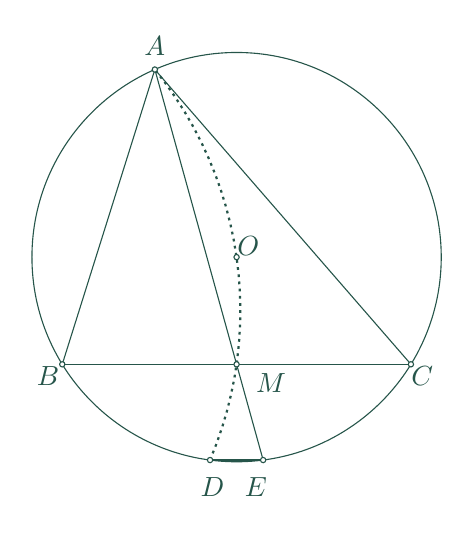
\begin{tikzpicture}[thachthuctoanhoc,scale=0.6]
			\draw  (-3.26,4.44)-- (-5.22,-1.8);
			\draw  (-5.22,-1.8)-- (2.16,-1.8);
			\draw  (2.16,-1.8)-- (-3.26,4.44);
			\draw  (-1.53,0.4687820512820516) circle (4.331682351721972cm);
			\draw  (-2.0917832603951787,-3.826316499922491)-- (-0.9682167396048218,-3.8263164999224912);
			\draw  (-3.26,4.44)-- (-0.9682167396048218,-3.8263164999224912);
			\draw [shift={(-9.556965317919069,-0.665608974358972)},line width=0.8pt,dash pattern=on 1pt off 1.6pt]  plot[domain=-0.40050890991965815:0.6812945286306901,variable=\t]({1*8.106726541220599*cos(\t r)+0*8.106726541220599*sin(\t r)},{0*8.106726541220599*cos(\t r)+1*8.106726541220599*sin(\t r)});
			\draw [fill=white] (-3.26,4.44) circle (1.6pt);
			\draw (-3.26,4.93) node {$A$};
			\draw [fill=white] (-5.22,-1.8) circle (1.6pt);
			\draw (-5.52,-2.05) node {$B$};
			\draw [fill=white] (2.16,-1.8) circle (1.6pt);
			\draw (2.4,-2.05) node {$C$};
			\draw [fill=white] (-1.53,0.4687820512820516) circle (1.6pt);
			\draw (-1.28,0.71) node {$O$};
			\draw [fill=white] (-1.53,-1.8) circle (1.6pt);
			\draw (-0.8,-2.2) node {$M$};
			\draw [fill=white] (-2.0917832603951787,-3.826316499922491) circle (1.6pt);
			\draw (-2.04,-4.4) node {$D$};
			\draw [fill=white] (-0.9682167396048218,-3.8263164999224912) circle (1.6pt);
			\draw (-1.12,-4.4) node {$E$};
		\end{tikzpicture}
	\end{center}
	\begin{flushright}
		\textit{Bằng Linh, Phú Thọ (st)}
	\end{flushright}
	{\color{thachthuctoanhoc}{\usefont{T5}{qag}{b}{n} P716.}}
	(Mức $B$) Trong một lớp học có $33$ học sinh. Mỗi bạn viết lên bảng số người trong lớp có cùng tên với mình và viết lên bảng số người có cùng họ với mình. Sau khi tất cả học sinh hoàn thành việc viết số, thì trên bảng các số $0,1,2,\ldots,10$ đều xuất hiện ít nhất một lần. Hỏi số $6$ xuất hiện bao nhiêu lần?
	\begin{flushright}
		\textit{Tô Trung Hiếu, Nghệ An (st)}
	\end{flushright}
	{\color{thachthuctoanhoc}{\usefont{T5}{qag}{b}{n} P717.}}
	(Mức $A$) Chứng minh rằng, với mọi bộ ba số thực $(a;b;c)$ thoả mãn  $ac\ne0$ và $b^2\ge4ac$, ta có
	\begin{align*}
		(a-b)^4+(b-c)^4+(c-a)^4 \ge \dfrac{81}{128}c^4.
	\end{align*}
	\begin{flushright}
		\textit{Nguyễn Văn Long, Vĩnh Phúc}
	\end{flushright}
	{\color{thachthuctoanhoc}{\usefont{T5}{qag}{b}{n} P718.}}
	(Mức $A$) Cho tam giác $ABC$ và $P$ là một điểm cố định nằm trong tam giác đó. Một đường thẳng $d$ quay quanh điểm $P$, cắt các đường thẳng $BC,CA,AB$ tương ứng tại các điểm $D,E,F$. Gọi $Q$ là giao điểm thứ hai của hai đường tròn $(ADE)$ và $(APF)$. Chứng minh rằng, $Q$ luôn thuộc một đường tròn cố định.  
	\begin{center}
		\definecolor{ffqqqq}{rgb}{1,0,0}
		\definecolor{qqqqff}{rgb}{0,0,1}
		\definecolor{qqqqffa}{rgb}{1,1,1}
		\begin{tikzpicture}[thachthuctoanhoc, scale=0.7]
			\draw  (-4.76,5.36)-- (-6.22,-0.5);
			\draw  (-6.22,-0.5)-- (0.2,-0.5);
			\draw  (0.2,-0.5)-- (-4.76,5.36);
			\draw [color=ffqqqq] (-5.222691037714135,1.894862071043978) circle (3.4958924272738447cm);
			\draw  (-5.750222132850728,2.8374132314498297) circle (2.709978575054024cm);
			\draw  (-7.76943396226415,-0.5)-- (-1.7287290671233002,1.7787000672061575);
			\draw  (-7.76943396226415,-0.5)-- (-6.22,-0.5);
			\draw [fill=white] (-4.76,5.36) circle (1.6pt);
			\draw (-4.76,5.73) node {$A$};
			\draw [fill=white] (-6.22,-0.5) circle (1.6pt);
			\draw (-6.36,-0.87) node {$B$};
			\draw [fill=white] (0.2,-0.5) circle (1.6pt);
			\draw (0.26,-0.81) node {$C$};
			\draw [fill=white] (-3.74,1.02) circle (1.6pt);
			\draw (-3.5,0.65) node {$P$};
			\draw [fill=white] (-7.76943396226415,-0.5) circle (1.6pt);
			\draw (-8.1,-0.73) node {$D$};
			\draw [fill=white] (-1.7287290671233002,1.7787000672061575) circle (1.6pt);
			\draw (-1.34,1.95) node {$E$};
			\draw [fill=white] (-6.059271801059053,0.14511455191366746) circle (1.6pt);
			\draw (-6.3,0.5) node {$F$};
			\draw [fill=white] (-8.418223065252786,3.3125499506724045) circle (1.6pt);
			\draw (-8.82,3.53) node {$Q$};
		\end{tikzpicture}
	\end{center}
	\begin{flushright}
		\textit{Phạm Vĩnh Minh, Đồng Tháp}
	\end{flushright}
	{\color{thachthuctoanhoc}{\usefont{T5}{qag}{b}{n} P719.}}
	(Mức $A$) Cho $S$ là một tập hữu hạn các số nguyên lớn hơn $1$ thoả mãn: với mỗi số nguyên dương $n$, tồn tại $x\in S$ sao cho  hoặc $x,n$ nguyên tố cùng nhau, hoặc $n$ chia hết cho $x$.  Chứng minh rằng, tồn tại $x,y\in S$ (có thể trùng nhau) sao cho $\gcd(x,y)$ là một số nguyên tố. 
	\begin{flushright}
		\textit{Bằng Linh, Phú Thọ (st)}
	\end{flushright}
	{\color{thachthuctoanhoc}{\usefont{T5}{qag}{b}{n} P720.}}
	(Mức $A$) Trong một thành phố, có $1334$ căn nhà. Mỗi dịp Noel, ông già Noel sẽ đến thăm các căn nhà đó theo thứ tự tùy ý. Chứng minh rằng, trong $3$ năm liên tiếp ta luôn tìm được $12$ căn nhà được ông già Noel đến thăm theo cùng một thứ tự như nhau (theo thời gian trước -- sau) ở $2$ năm trong số $3$ năm đó. 
	\begin{flushright}
		\textit{Trương Bảo Nam, Hà Nội}
	\end{flushright}
\end{multicols}
%\centerline{{\large{\textbf{\color{thachthuctoanhoc}GIẢI BÀI KỲ TRƯỚC}}}}
%\vspace*{-5pt}
%\begin{multicols}{2}
%	\setlength{\abovedisplayskip}{4pt}
%	\setlength{\belowdisplayskip}{4pt}
%	{\color{thachthuctoanhoc}{\usefont{T5}{qag}{b}{n} P671.}}
%	(Mức $B$) Một hình chữ nhật được chia thành $9$ hình chữ nhật con như hình vẽ. Số ghi ở giữa mỗi hình chữ nhật con bằng chu vi của hình chữ nhật ấy. Biết rằng $c$ là một số nguyên khác $2,3,4,5$; hãy tìm $a,b,c,d,e$.
%	\begin{figure}[H]
%		\vspace*{5pt}
%		\centering
%		\captionsetup{labelformat= empty, justification=centering}
%		\begin{tikzpicture}[yscale=1.1, scale=0.78,thachthuctoanhoc]
%			\draw (0,0) rectangle (9,3); 
%			\draw (2,0) -- (2, 3) (6, 0) -- (6, 3);
%			\draw (0,1.2) -- (9, 1.2) (0, 2.1) -- (9, 2.1);
%			\draw (1,2.5) node{$a$};
%			\draw (1,1.65) node{$2$};
%			\draw (1,0.6) node{$d$};
%			\draw (4,2.5) node{$4$};
%			\draw (4,1.65) node{$c$};
%			\draw (4,0.6) node{$5$};
%			\draw (7.5,2.5) node{$b$};
%			\draw (7.5,1.65) node{$3$};
%			\draw (7.5,0.6) node{$e$};
%		\end{tikzpicture}
%		\vspace*{-5pt}
%	\end{figure}
%	\textbf{\color{thachthuctoanhoc}Lời giải} (\textit{dựa theo lời giải của bạn Hà Mạnh Hùng, lớp $8$A, trường THPT chuyên Hà Nội -- Amsterdam, Tp. Hà Nội})\textbf{\color{thachthuctoanhoc}.}
%	\vskip 0.05cm
%	Trước hết, ta có Nhận xét đơn giản sau:
%	\vskip 0.05cm
%	\textbf{\color{thachthuctoanhoc}\textit{Nhận xét.}} Nếu một hình chữ nhật được phân chia thành bốn hình chữ nhật I, II, III, IV như ở hình dưới đây, thì tổng chu vi của hai hình chữ nhật I và IV bằng tổng chu vi của hai hình chữ nhật II và III.
%	\begin{figure}[H]
%		\vspace*{-5pt}
%		\centering
%		\captionsetup{labelformat= empty, justification=centering}
%		\begin{tikzpicture}[thachthuctoanhoc]
%			\draw (0,0) rectangle (5,2);
%			\draw (0,1.2) -- (5,1.2) (2,0) -- (2,2);
%			\draw (1,0.6) node{III};	
%			\draw (1,1.6) node{I};
%			\draw (3.5,0.6) node{IV};
%			\draw (3.5,1.6) node{II};	
%		\end{tikzpicture}
%		\vspace*{-10pt}
%	\end{figure}
%	Theo Nhận xét trên, từ các giả thiết của bài ra về chu vi của $9$ hình chữ nhật con, ta có:
%	\begin{align*}
%		\quad\quad\begin{cases}
%			a + c = 4 + 2 = 6 \hspace*{67pt} (1)\\[-0.5ex]
%			b + c = 4 + 3 = 7 \hfill (2)\\[-0.5ex]
%			c + e = 3 + 5 = 8 \hfill (3)\\[-0.5ex]
%			c + d = 2 + 5 = 7. \hfill (4)
%		\end{cases}
%	\end{align*}
%	Từ ($1$), do $a > 0$, suy ra $0 < c < 6$. Mà $c$ là một số nguyên, khác $2$, $3$, $4$, $5$ (giả thiết), nên $c = 1$. Từ đây và ($1$), ($2$), ($3$), ($4$), lần lượt suy ra, $a = 6 - 1 = 5$, $b = 7 - 1 = 6$, $e = 8 - 1 = 7$, $d = 7 - 1 = 6$.
%	\vskip 0.05cm
%	Vậy, $a = 5$, $b = 6$, $c = 1$, $d = 6$, $e = 7$.
%	\vskip 0.05cm
%	\textbf{\color{thachthuctoanhoc}Bình luận và Nhận xét}
%	\vskip 0.05cm
%	Trong số các lời giải Tạp chí đã nhận được, rất tiếc, có một lời giải không được coi là lời giải hoàn chỉnh, do người giải bài vẫn đang dang dở trong các lập luận lý giải cho kết quả tìm được.
%	\vskip 0.05cm
%	\hfill\textbf{\color{thachthuctoanhoc}Lê Huy}
%	\vskip 0.05cm
%	{\color{thachthuctoanhoc}{\usefont{T5}{qag}{b}{n} P672.}}
%	(Mức $B$) Cho $x$ và $y$ là các số nguyên dương phân biệt thoả mãn
%	\begin{align*}
%		2023x^{2023}+999 y^{2023}
%	\end{align*}
%	chia hết cho $x+y$. Chứng minh rằng $x+y$ là hợp số. 
%	\vskip 0.05cm
%	\textbf{\color{thachthuctoanhoc}Lời giải} (\textit{phỏng theo Đáp án của bài toán})\textbf{\color{thachthuctoanhoc}.}
%	\vskip 0.05cm
%	Ta có:
%	\begin{align*}
%		&2023{x^{2023}} + 999{y^{2023}} \\[-0.5ex]
%		= \,\,&999\left( {{x^{2023}} + {y^{2023}}} \right) + {2^{10}} \cdot {x^{2023}}.\tag{$1$}
%	\end{align*}
%	Do $2023$ là số lẻ, nên $\left( {{x^{2023}} + {y^{2023}}} \right) \vdots \left( {x + y} \right)$. Vì thế, từ giả thiết của bài toán và ($1$), suy ra
%	\begin{align*}
%		{2^{10}} \cdot {x^{2023}} \,\vdots \left( {x + y} \right).\tag{$2$}
%	\end{align*}
%	Vì $x, y$ là hai số nguyên dương phân biệt, nên $x + y \ge  3 > 1$. Do đó, $x + y$ hoặc là số nguyên tố lẻ, hoặc là hợp số.  
%	\hfill ($3$)
%	\vskip 0.05cm
%	Nếu $x + y$ là số nguyên tố lẻ thì $\left( {{2^{10}},x + y} \right) = 1$.  Vì thế, từ ($2$) ta có
%	\begin{align*}
%		{x^{2023}} \,\vdots \left( {x + y} \right).
%	\end{align*}
%	Mà $x + y$ là số nguyên tố nên $x \,\vdots \left( {x + y} \right)$.  Suy ra, $x \ge  x + y$ (do $x, x + y \in \mathbb{N^*}$), là điều vô lý (do $y > 0$). Vì vậy, $x + y$ không thể là số nguyên tố lẻ. Từ đây và ($3$) suy ra, $x + y$ là hợp số.
%	\vskip 0.05cm
%	Ta có điều phải chứng minh theo yêu cầu đề bài.
%	\vskip 0.05cm
%	\textbf{\color{thachthuctoanhoc}Bình luận và Nhận xét}
%	\vskip 0.05cm
%	$\pmb{1.}$ Trong lời giải trên, ta đã sử dụng kết quả rất quen biết sau:
%	\vskip 0.05cm
%	``Với mọi $n \in \mathbb{N}$, với mọi  $a,b \in \mathbb{Z}$, mà $a + b \ne  0, \pm 1$, luôn có  $\left( {{a^{2n + 1}} + {b^{2n + 1}}} \right) \vdots \left( {a + b} \right).$"
%	\vskip 0.05cm
%	Các bạn đọc chưa biết kết quả trên có thể dễ dàng chứng minh được kết quả đó, bằng cách sử dụng phân tích của ${a^{2n + 1}} + {b^{2n + 1}}$ thành thừa số.
%	\vskip 0.05cm
%	$\pmb{2.}$ Tất cả các lời giải Tạp chí nhận được từ bạn đọc đều mắc \textit{lỗi logic} sau: Khẳng định, với $a \in \mathbb{N^*}$, nếu $a$ không là số nguyên tố thì $a$ là hợp số.
%	\vskip 0.05cm
%	Lưu ý rằng, \textit{$1$ không phải là số nguyên tố, và cũng không phải là hợp số}! Vì thế, để từ ``$a \in \mathbb{N^*}$  và $a$ không là số nguyên tố" có thể suy ra ``$a$ là hợp số", cần có thêm điều kiện $a > 1$.
%	\vskip 0.05cm
%	Người chấm bài đã châm chước lỗi trên, khi đánh giá tính đúng và tính hoàn chỉnh của lời giải.
%	\vskip 0.05cm
%	$\pmb{3.}$ Với sự châm chước nêu trên, trong số các lời giải Tạp chí nhận được từ bạn đọc, rất tiếc, vẫn có một số lời giải không được chấp nhận là lời giải hoàn chỉnh, do người giải bài không có các giải thích cần thiết cho một số sự kiện thiết yếu của lời giải.
%	\vskip 0.05cm
%	\hfill\textbf{\color{thachthuctoanhoc}Lưu Thị Thanh Hà}
%	\vskip 0.05cm
%	{\color{thachthuctoanhoc}{\usefont{T5}{qag}{b}{n} P673.}}
%	(Mức $B$) Chứng minh rằng,
%	\begin{align*}
%		A\!=\!\sqrt[3]{1^3\!+\!1}\!+\!\sqrt[3]{2^3\!+\!1}\!+\!\cdots\!+\!\sqrt[3]{2023^3\!+\!1}
%	\end{align*}
%	không phải là số nguyên.
%	\vskip 0.05cm
%	\textbf{\color{thachthuctoanhoc}Lời giải} (\textit{dựa theo lời giải của bạn Hà Mạnh Hùng, lớp $8$A, trường THPT chuyên Hà Nội -- Amsterdam, Tp. Hà Nội})\textbf{\color{thachthuctoanhoc}.}
%	\vskip 0.05cm
%	Đặt $A = \sqrt[3]{{{1^3} + 1}} + \sqrt[3]{{{2^3} + 1}} +  \cdots  + \sqrt[3]{{{{2023}^3} + 1}},$  và $B = 1 + 2 +  \cdots  + 2023$.
%	\vskip 0.05cm 
%	Vì với mọi  $n \in \mathbb{N^*}, \sqrt[3]{{{n^3} + 1}} > \sqrt[3]{{{n^3}}} = n$, nên $A > B$. \hfill ($1$)
%	\vskip 0.05cm      
%	Tiếp theo, với mọi $n \in \mathbb{N^*}$, do ${n^2} + n < 3{n^2},$  nên
%	\begin{align*}
%		{n^3} \!+\! 1 \!<\! {n^3} \!+\! \frac{{3{n^2}}}{{n\left( {n \!+\! 1} \right)}} \!<\! {\left( {n \!+\! \frac{1}{{n\left( {n \!+\! 1} \right)}}} \right)^3}\!.
%	\end{align*}
%	Suy ra
%	\begin{align*}
%		\sqrt[3]{{{n^3} \!+\! 1}} \!<\! n \!+\! \frac{1}{{n\left( {n \!+\! 1} \right)}} \!=\! n \!+\! \left( {\frac{1}{n} \!-\! \frac{1}{{n \!+\! 1}}} \right)\!,
%	\end{align*}
%	với mọi $n \in \mathbb{N^*}$.
%	\vskip 0.05cm  
%	Vì thế
%	\begin{align*}
%		A <\,& B + \left( \left( {\frac{1}{1} - \frac{1}{2}} \right) + \left( {\frac{1}{2} - \frac{1}{3}} \right) +  \cdots\right.  \\
%			&\left.+ \left( {\frac{1}{{2023}} - \frac{1}{{2024}}} \right) \right) \\
%		= \,&B + \left( {1 - \frac{1}{{2024}}} \right) < B + 1. \tag{$2$}
%	\end{align*}
%	Từ ($1$) và ($2$), ta có $B < A < B + 1$. Mà $B$ là số nguyên, nên $A$ không là số nguyên.
%	\vskip 0.05cm
%	Ta có điều phải chứng minh theo yêu cầu đề bài.
%	\vskip 0.05cm
%	\textbf{\color{thachthuctoanhoc}Bình luận và Nhận xét}
%	\vskip 0.05cm
%	$\pmb{1.}$ Ngoài cách đã nêu ở Lời giải trên, còn có thể chứng minh $A < B + 1$ (theo ký hiệu ở Lời giải) bằng cách sử dụng đánh giá sau:
%	\begin{align*}
%		\sqrt[3]{{{n^3} + 1}} < n + \frac{1}{{3{n^2}}}, \text{ với mọi } n \in \mathbb{N^*}.
%	\end{align*}
%	$\pmb{2.}$ Trong số các lời giải Tạp chí đã nhận được từ bạn đọc, rất tiếc có một lời giải sai (do người giải bài đã tính sai tổng các số tự nhiên từ $2$ đến $2024$) và một lời giải \textit{không} được chấp nhận là đầy đủ và chính xác (do người giải bài đã bỏ qua quá nhiều các tính toán cụ thể cần thiết).
%	\vskip 0.05cm
%		\hfill\textbf{\color{thachthuctoanhoc}Lê Huy}
%	\vskip 0.05cm
%	{\color{thachthuctoanhoc}{\usefont{T5}{qag}{b}{n} P674.}}
%	(Mức $B$) Ở mỗi ô vuông con của bảng ô vuông $8\times8$ được điền một số $+1$, hoặc một số $-1$, sao cho tổng của bốn số ở một bảng con $2\times2$ tuỳ ý bằng $2$, hoặc $-2$. Chứng minh rằng, trong bảng số thu được có hai hàng giống nhau.
%	\vskip 0.05cm
%	\textbf{\color{thachthuctoanhoc}Lời giải} (\textit{của người chấm bài})\textbf{\color{thachthuctoanhoc}.}
%	\vskip 0.05cm
%	Ở lời giải này:
%	\vskip 0.05cm
%	-- $\left( {{x_1},{x_2}, \ldots ,{x_8}} \right)$ ký hiệu hàng, mà các ô vuông con của nó, lần lượt từ trái qua phải, được điền các số  ${x_1},{x_2}, \ldots ,{x_8}.$
%	\vskip 0.05cm
%	-- $\left(\!\!\! \begin{array}{l}
%		x\,\,\,\, u\\
%		y\,\,\,\, v
%	\end{array}\!\!\! \right)$  ký hiệu bảng $2 \times  2$, mà các ô vuông con của nó, lần lượt từ trên xuống dưới, từ trái qua phải, được điền các số $x, y, u, v$.
%	\vskip 0.05cm
%	-- Cặp gồm hàng thứ $m$ và hàng thứ $n$ sẽ được gọi vắn tắt là \textit{cặp} $m - n$.
%	\vskip 0.05cm
%	Ta có các Nhận xét sau:
%	\vskip 0.05cm
%	\textbf{\color{thachthuctoanhoc}Nhận xét} $\pmb{1.}$ Giả sử các ô vuông con của một bảng con $2 \times  2$ tùy ý của bảng $8 \times  8$ đã cho, theo thứ tự từ trên xuống dưới, từ trái qua phải, lần lượt được điền các số $a, b, c, d$ (xem Hình $1$).
%	\begin{table}[H]
%		\vspace*{-10pt}
%		\centering
%		\captionsetup{labelformat= empty, justification=centering}
%		\renewcommand{\arraystretch}{1.2}
%		\setlength{\tabcolsep}{7pt}
%			\begin{tabular}{|c|c|}
%				\hline
%				$a$ & $c$\\
%				\hline
%				$b$ & $d$\\
%				\hline
%			\end{tabular}
%		\caption{\small\textit{\color{thachthuctoanhoc}Hình $1$.}}
%		\vspace*{-10pt}
%	\end{table}
%	Khi đó:
%	\vskip 0.05cm
%	-- Nếu $a = b$ thì $c = -d$;
%	\vskip 0.05cm
%	-- Nếu $a = -b$ thì $c = d$.
%	\vskip 0.05cm
%	\textit{Chứng minh.} Theo giả thiết của bài ra, $a, b, c, d \in  \{+1; -1\}$ và $(a + b + c + d) \in  \{2; -2\}$. Suy ra, trong bốn số $a,b,c,d$, hoặc có ba số bằng $1$ và số còn lại bằng $-1$, hoặc có ba số bằng $-1$ và số còn lại bằng $1$. Do đó, $abcd = -1$. Vì vậy:
%	\vskip 0.05cm
%	-- Nếu $a = b$ thì $cd = -1$ (do $ab = {a^2} = 1$); suy ra, $c = -d$.
%	\vskip 0.05cm
%	-- Nếu $a = -b$ thì $cd = 1$ (do $ab =  - {a^2} =  - 1$); suy ra, $c = d$.
%	\vskip 0.05cm
%	Nhận xét $1$ được chứng minh.
%	\vskip 0.05cm
%	\textbf{\color{thachthuctoanhoc}Nhận xét} $\pmb{2.}$ Giả sử $\left( {{x_1},{x_2}, \ldots ,{x_8}} \right)$ và $\left( {{y_1},{y_2}, \ldots ,{y_8}} \right)$ là hai hàng liên tiếp của bảng $8 \times  8$ đã cho (xem Hình $2$).
%	\begin{table}[H]
%		\vspace*{-10pt}
%		\centering
%		\captionsetup{labelformat= empty, justification=centering}
%		\renewcommand{\arraystretch}{1.2}
%		\setlength{\tabcolsep}{7pt}
%		\begin{tabular}{|c|c|c|c|c|c|c|c|c|}
%			\hline
%			$x_1$ & $x_2$ & $x_3$ & $x_4$ & $x_5$ & $x_6$ & $x_7$ & $x_8$ \\
%			\hline
%			$y_1$ & $y_2$ & $y_3$ & $y_4$ & $y_5$ & $y_6$ & $y_7$ & $y_8$ \\
%			\hline
%		\end{tabular}
%		\caption{\small\textit{\color{thachthuctoanhoc}Hình $2$.}}
%		\vspace*{-15pt}
%	\end{table}
%	Khi đó:
%	\vskip 0.05cm
%	-- Nếu ${x_1} \!=\! {y_1}$ thì ${x_i} \!=\! {y_i}$  với mọi $i \!\in\!  \{\!1;\! 3;\! 5; \!7\!\}$, và ${x_i} =  - {y_i}$  với mọi $i \in  \{2; 4; 6; 8\}$;
%	\vskip 0.05cm
%	-- Nếu ${x_1} =  - {y_1}$ thì ${x_i} = {y_i}$ với mọi $i \in  \{2; 4; 6; 8\}$, và  ${x_i} =  - {y_i}$ với mọi \linebreak$i \in  \{1; 3; 5; 7\}$.
%	\vskip 0.05cm
%	\textit{Chứng minh.}
%	\vskip 0.05cm
%	-- Giả sử  $x_1 = y_1$. Khi đó, áp dụng Nhận xét $1$, lần lượt, cho  $\left(\!\!\! \begin{array}{l}
%		{x_1}\,\,\,\,{x_2}\\
%		{y_1}\,\,\,\,{y_2}
%	\end{array} \!\!\!\right)$,  $\left(\!\!\! \begin{array}{l}
%	{x_2}\,\,\,\,{x_3}\\
%	{y_2}\,\,\,\,{y_3}
%\end{array} \!\!\!\right)$,  $\left(\!\!\! \begin{array}{l}
%{x_3}\,\,\,\,{x_4}\\
%{y_3}\,\,\,\,{y_4}
%\end{array} \!\!\!\right)$,
%$\left(\!\!\!\! \begin{array}{l}
%	{x_4}\,\,\,\,{x_5}\\
%	{y_4}\,\,\,\,{y_5}
%\end{array} \!\!\!\right)$,
% $\left(\!\!\! \begin{array}{l}
%{x_5}\,\,\,\,{x_6}\\
%{y_5}\,\,\,\,{y_6}
%\end{array} \!\!\!\right)$,  $\left(\!\!\! \begin{array}{l}
%{x_6}\,\,\,\,{x_7}\\
%{y_6}\,\,\,\,{y_7}
%\end{array} \!\!\!\right)$,  $\left(\!\!\! \begin{array}{l}
%{x_7}\,\,\,\,{x_8}\\
%{y_7}\,\,\,\,{y_8}
%\end{array} \!\!\!\right)$,  ta được:
%	\begin{align*}
%		&{x_2} =  - {y_2}, x_3 = y_3, x_4 = - y_4, x_5 = y_5,\\
%		&x_6 = -y_6, x_7 = y_7, x_8 = -y_8.
%	\end{align*}
%	-- Giả sử  $x_1 = -y_1$. Khi đó, áp dụng Nhận xét $1$, lần lượt, cho bảy bảng con $2 \times  2$ vừa nêu trên, ta được:
%	\begin{align*}
%		&x_2 = y_2, x_3 = -y_3, x_4 = y_4, x_5 = -y_5,\\
%		&x_6 = y_6, x_7 = -y_7, x_8 = y_8.
%	\end{align*}
%	Nhận xét $2$ được chứng minh.
%	\vskip 0.05cm
%	Ta gọi cặp gồm hai hàng liên tiếp,  $\left( {{x_1},{x_2}, \ldots ,{x_8}} \right)$ và  $\left( {{y_1},{y_2}, \ldots ,{y_8}} \right)$, là một \textit{cặp xanh}, nếu  $x_1 = y_1$; và gọi cặp gồm hai hàng đó là một \textit{cặp đỏ}, nếu  $x_1 = -y_1$.
%	\vskip 0.05cm
%	Trong phần trình bày dưới đây, thứ tự của các hàng được tính từ trên xuống dưới.
%	\vskip 0.05cm
%	Với bảng $8 \times  8$ đã cho, xảy ra đúng một trong hai trường hợp sau:
%	\vskip 0.05cm
%	$\diamond$ \textit{Trường hợp} $1$: Tồn tại ba hàng liên tiếp mà cặp $1 - 2$ và cặp $2 - 3$ là hai cặp cùng màu.
%	\vskip 0.05cm
%	Giả sử $\left( {{a_1},{a_2}, \ldots ,{a_8}} \right)$  là hàng thứ nhất trong ba hàng đó. Khi đó, theo Nhận xét $2$, ba hàng này sẽ hoặc là ba hàng ở Hình $3$, hoặc là ba hàng ở Hình $4$.
%	\begin{table}[H]
%		\vspace*{-5pt}
%		\centering
%		\captionsetup{labelformat= empty, justification=centering}
%		\renewcommand{\arraystretch}{1.2}
%		\setlength{\tabcolsep}{4.5pt}
%		\begin{tabular}{|c|c|c|c|c|c|c|c|c|}
%			\hline
%			$a_1$ & $a_2$ & $a_3$ & $a_4$ & $a_5$ & $a_6$ & $a_7$ & $a_8$ \\
%			\hline
%			$a_1$ & $-a_2$ & $a_3$ & $-a_4$ & $a_5$ & $-a_6$ & $a_7$ & $-a_8$ \\
%			\hline
%			$a_1$ & $a_2$ & $a_3$ & $a_4$ & $a_5$ & $a_6$ & $a_7$ & $a_8$ \\
%			\hline
%		\end{tabular}
%		\caption{\small\textit{\color{thachthuctoanhoc}Hình $3$. Cặp $1 - 2$ và cặp $2 - 3$ cùng là cặp xanh.}}
%		\vspace*{-10pt}
%	\end{table}
%	\begin{table}[H]
%		\vspace*{-5pt}
%		\centering
%		\captionsetup{labelformat= empty, justification=centering}
%		\renewcommand{\arraystretch}{1.2}
%		\setlength{\tabcolsep}{4.5pt}
%		\begin{tabular}{|c|c|c|c|c|c|c|c|c|}
%			\hline
%			$a_1$ & $a_2$ & $a_3$ & $a_4$ & $a_5$ & $a_6$ & $a_7$ & $a_8$ \\
%			\hline
%			$-a_1$ & $a_2$ & $-a_3$ & $a_4$ & $-a_5$ & $a_6$ & $-a_7$ & $a_8$ \\
%			\hline
%			$a_1$ & $a_2$ & $a_3$ & $a_4$ & $a_5$ & $a_6$ & $a_7$ & $a_8$ \\
%			\hline
%		\end{tabular}
%		\caption{\small\textit{\color{thachthuctoanhoc}Hình $4$. Cặp $1 - 2$ và cặp $2 - 3$ cùng là cặp đỏ.}}
%		\vspace*{-10pt}
%	\end{table}
%	Nhận thấy, hàng thứ nhất và hàng thứ ba ở mỗi hình (trong hai hình, $3$ và $4$) là hai hàng giống nhau. Điều này cho thấy, trong bảng $8 \times 8$ đã cho có hai hàng giống nhau.
%	\vskip 0.05cm
%	$\diamond$ \textit{Trường hợp} $2$: Với ba hàng liên tiếp bất kỳ, cặp $1 - 2$ và cặp $2 - 3$ là hai cặp khác màu.
%	\vskip 0.05cm
%	Xét năm hàng đầu tiên của bảng $8 \times  8$ đã cho.
%	\vskip 0.05cm
%	Giả sử $\left( {{a_1},{a_2}, \ldots ,{a_8}} \right)$ là hàng thứ nhất trong năm hàng đó.
%	\vskip 0.05cm
%	Xảy ra một trong hai khả năng sau:
%	\vskip 0.05cm
%	-- \textit{Khả năng} $1$: Cặp $1 - 2$ là cặp xanh, và cặp $2 - 3$ là cặp đỏ.
%	\vskip 0.05cm
%	Khi đó, từ giả thiết ``khác màu" suy ra, cặp $3 - 4$ là cặp xanh, và cặp $4 - 5$ là cặp đỏ.
%	\vskip 0.05cm
%	Vì thế, ở khả năng này, theo Nhận xét $2$, năm hàng đầu tiên của bảng $8 \times  8$ đã cho là năm hàng dưới đây (xem Hình $5$):
%	\begin{table}[H]
%		\vspace*{-5pt}
%		\centering
%		\captionsetup{labelformat= empty, justification=centering}
%		\renewcommand{\arraystretch}{1.2}
%		\setlength{\tabcolsep}{2pt}
%		\begin{tabular}{|c|c|c|c|c|c|c|c|c|}
%			\hline
%			$a_1$ & $a_2$ & $a_3$ & $a_4$ & $a_5$ & $a_6$ & $a_7$ & $a_8$ \\
%			\hline
%			$a_1$ & $-a_2$ & $a_3$ & $-a_4$ & $a_5$ & $-a_6$ & $a_7$ & $-a_8$ \\
%			\hline
%			$-a_1$ & $-a_2$ & $-a_3$ & $-a_4$ & $-a_5$ & $-a_6$ & $-a_7$ & $-a_8$ \\
%			\hline
%			$-a_1$ & $a_2$ & $-a_3$ & $a_4$ & $-a_5$ & $a_6$ & $-a_7$ & $a_8$ \\
%			\hline
%			$a_1$ & $a_2$ & $a_3$ & $a_4$ & $a_5$ & $a_6$ & $a_7$ & $a_8$ \\
%			\hline
%		\end{tabular}
%		\caption{\small\textit{\color{thachthuctoanhoc}Hình $5$.}}
%		\vspace*{-10pt}
%	\end{table}
%	-- \textit{Khả năng} $2$: Cặp $1 - 2$ là cặp đỏ, và cặp $2 - 3$ là cặp xanh.
%	\vskip 0.05cm
%	Khi đó, từ giả thiết ``khác màu" suy ra, cặp $3 - 4$ là cặp đỏ, và cặp $4 - 5$ là cặp xanh.
%	\vskip 0.05cm
%	Vì thế, ở khả năng này, theo Nhận xét $2$, năm hàng đầu tiên của bảng $8 \times  8$ đã cho là năm hàng dưới đây (xem Hình $6$):
%	\begin{table}[H]
%		\vspace*{-10pt}
%		\centering
%		\captionsetup{labelformat= empty, justification=centering}
%		\renewcommand{\arraystretch}{1.2}
%		\setlength{\tabcolsep}{2pt}
%		\begin{tabular}{|c|c|c|c|c|c|c|c|c|}
%			\hline
%			$a_1$ & $a_2$ & $a_3$ & $a_4$ & $a_5$ & $a_6$ & $a_7$ & $a_8$ \\
%			\hline
%			$-a_1$ & $a_2$ & $-a_3$ & $a_4$ & $-a_5$ & $a_6$ & $-a_7$ & $a_8$ \\
%			\hline
%			$-a_1$ & $-a_2$ & $-a_3$ & $-a_4$ & $-a_5$ & $-a_6$ & $-a_7$ & $-a_8$ \\
%			\hline
%			$a_1$ & $-a_2$ & $a_3$ & $-a_4$ & $a_5$ & $-a_6$ & $a_7$ & $-a_8$ \\
%			\hline
%			$a_1$ & $a_2$ & $a_3$ & $a_4$ & $a_5$ & $a_6$ & $a_7$ & $a_8$ \\
%			\hline
%		\end{tabular}
%		\caption{\small\textit{\color{thachthuctoanhoc}Hình $6$.}}
%		\vspace*{-15pt}
%	\end{table}
%	Nhận thấy, hàng thứ nhất và hàng thứ năm ở mỗi hình, trong hai hình $5$ và $6$, là hai hàng giống nhau. Điều này cho thấy, dù khả năng nào xảy ra, trong bảng $8 \times  8$ đã cho đều có hai hàng giống nhau.
%	\vskip 0.05cm
%	Kết quả xét hai trường hợp trên đây cho ta điều phải chứng minh theo yêu cầu đề bài.
%	\vskip 0.05cm
%	\textbf{\color{thachthuctoanhoc}Bình luận và Nhận xét}
%	\vskip 0.05cm
%	$\pmb{1.}$ Lời giải trên được trình bày theo tinh thần giúp bạn đọc cảm nhận, hình dung được cách tiếp cận để tìm ra lời giải cho bài đã ra.
%	\vskip 0.05cm
%	$\pmb{2.}$ Lời giải trên cho thấy, kết quả của bài đã ra không thay đổi, khi thay bảng $8 \times  8$ bởi bảng $m \times  n$, với $m, n$ là các số nguyên dương tùy ý, thỏa mãn $m \ge  5$ và $n \ge  2$.
%	\vskip 0.05cm
%	$\pmb{3.}$ Rất tiếc, cho tới thời điểm bản thảo vào Nhà in, Tạp chí vẫn chưa nhận được lời giải nào, từ bạn đọc.
%	\vskip 0.05cm
%		\hfill\textbf{\color{thachthuctoanhoc}Nguyễn Khắc Minh}
%	\vskip 0.05cm
%	{\color{thachthuctoanhoc}{\usefont{T5}{qag}{b}{n} P675.}}
%	(Mức $B$) Cho hình thang $ABCD$ vuông tại $A$ và $D$. Trên tia $AD$ lấy điểm $F$ sao cho $AF\cdot AD=AB\cdot CD$. Gọi $E$ là hình chiếu vuông góc của $A$ trên $BD$. Chứng minh rằng $\angle CEF=90^\circ$. 
%	\vskip 0.05cm
%	\textbf{\color{thachthuctoanhoc}Lời giải} (\textit{của người chấm bài})\textbf{\color{thachthuctoanhoc}.}
%	\vskip 0.05cm
%	Từ các giả thiết của bài toán suy ra, $F \not\equiv A$  và $E$ nằm giữa $B$ và $D$.
%	
%	Vì $DA \bot  AB$ và $AE \bot  BD$ (giả thiết), nên
%	\begin{align*}
%		\angle ABD = \angle EAD
%	\end{align*}
%	(hai góc nhọn có cạnh tương ứng vuông góc).
%	\vskip 0.05cm
%	\begin{figure}[H]
%		%		\vspace*{-5pt}
%		\centering
%		\captionsetup{labelformat= empty, justification=centering}
%		\definecolor{qqwuqq}{rgb}{0.,0.39215686274509803,0.}
%		\definecolor{ffqqqq}{rgb}{1.,0.,0.}
%		\definecolor{uuuuuu}{rgb}{0.26666666666666666,0.26666666666666666,0.26666666666666666}
%		\definecolor{xdxdff}{rgb}{0.49019607843137253,0.49019607843137253,1.}
%		\definecolor{qqqqff}{rgb}{0.,0.,1.}
%		\begin{tikzpicture}[thachthuctoanhoc,scale=0.65]
%			\draw[pattern color=qqwuqq,fill=qqwuqq,fill opacity=0.10000000149011612] (-0.7171572875253809,-1.) -- (-0.7171572875253809,-0.7171572875253809) -- (-1.,-0.7171572875253809) -- (-1.,-1.) -- cycle; 
%			\draw[pattern color=qqwuqq,fill=qqwuqq,fill opacity=0.10000000149011612] (-1.,4.717157287525381) -- (-0.7171572875253809,4.717157287525381) -- (-0.7171572875253809,5.) -- (-1.,5.) -- cycle; 
%			\draw[pattern color=qqwuqq,fill=qqwuqq,fill opacity=0.10000000149011612] (1.2261721636920768,4.385900396029219) -- (0.9647782966637699,4.493943194400919) -- (0.8567354982920697,4.232549327372612) -- (1.1181293653203765,4.124506529000912) -- cycle; 
%			\draw[pattern color=ffqqqq,fill=ffqqqq,fill opacity=0.10000000149011612] (0.9133399364577741,3.9294135003552704) -- (1.1084329651034157,3.7246240714926677) -- (1.3132223939660181,3.919717100138309) -- (1.1181293653203765,4.124506529000912) -- cycle; 
%			\draw [shift={(-1.,-1.)},pattern color=qqwuqq,fill=qqwuqq,fill opacity=0.10000000149011612] (0,0) -- (0.:0.6) arc (0.:67.54306100005789:0.6) -- cycle;
%			\draw [shift={(-1.,5.)},pattern color=qqwuqq,fill=qqwuqq,fill opacity=0.10000000149011612] (0,0) -- (-90.:0.6) arc (-90.:-22.4569389999421:0.6) -- cycle;
%			\draw [shift={(1.48,5.)},pattern color=qqwuqq,fill=qqwuqq,fill opacity=0.10000000149011612] (0,0) -- (180.:0.6) arc (180.:247.54306100005786:0.6) -- cycle;
%			\draw [shift={(-1.,2.106666666666665)},pattern color=ffqqqq,fill=ffqqqq,fill opacity=0.10000000149011612] (0,0) -- (43.61095691542593:0.6) arc (43.61095691542593:90.:0.6) -- cycle;
%			\draw [shift={(6.,-1.)},pattern color=ffqqqq,fill=ffqqqq,fill opacity=0.10000000149011612] (0,0) -- (133.6109569154259:0.6) arc (133.6109569154259:180.:0.6) -- cycle;
%			\draw [] (-1.,5.)-- (-1.,-1.);
%			\draw [] (-1.,-1.)-- (6.,-1.);
%			\draw [] (1.48,5.)-- (-1.,-1.);
%			\draw [color=ffqqqq] (-1.,2.106666666666665)-- (1.1181293653203765,4.124506529000912);
%			\draw [color=ffqqqq] (1.1181293653203765,4.124506529000912)-- (6.,-1.);
%			\draw [] (1.48,5.)-- (6.,-1.);
%			\draw [] (1.1181293653203765,4.124506529000912)-- (-1.,5.);
%			\draw [] (-1.,5.)-- (1.48,5.);
%			\draw (-1.46,5.9) node[anchor=north west] {$A$};
%			\draw (1.4,5.88) node[anchor=north west] {$B$};
%			\draw (6.,-0.76) node[anchor=north west] {$C$};
%			\draw (-1.84,-0.76) node[anchor=north west] {$D$};
%			\draw (1.12,4.72) node[anchor=north west] {$E$};
%			\draw (-1.86,2.64) node[anchor=north west] {$F$};
%			\draw [shift={(-1.,-1.)},color=qqwuqq] (0.:0.6) arc (0.:67.54306100005789:0.6);
%			\draw [shift={(-1.,-1.)},color=qqwuqq] (0.:0.5) arc (0.:67.54306100005789:0.5);
%			\draw [shift={(-1.,5.)},color=qqwuqq] (-90.:0.6) arc (-90.:-22.4569389999421:0.6);
%			\draw [shift={(-1.,5.)},color=qqwuqq] (-90.:0.5) arc (-90.:-22.4569389999421:0.5);
%			\draw [shift={(1.48,5.)},color=qqwuqq] (180.:0.6) arc (180.:247.54306100005786:0.6);
%			\draw [shift={(1.48,5.)},color=qqwuqq] (180.:0.5) arc (180.:247.54306100005786:0.5);
%			\draw [shift={(-1.,2.106666666666665)},color=ffqqqq] (43.61095691542593:0.6) arc (43.61095691542593:90.:0.6);
%			\draw[color=ffqqqq] (-0.8281584739762546,2.6185948744593506) -- (-0.7899714681932001,2.7323566984132803);
%			\draw[color=ffqqqq] (-0.7478725864649683,2.5841933856512007) -- (-0.6918442723460726,2.690310434314431);
%			\draw [shift={(6.,-1.)},color=ffqqqq] (133.6109569154259:0.6) arc (133.6109569154259:180.:0.6);
%			\draw[color=ffqqqq] (5.4880717922073154,-0.8281584739762551) -- (5.374309968253385,-0.7899714681932007);
%			\draw[color=ffqqqq] (5.522473281015465,-0.7478725864649689) -- (5.416356232352236,-0.6918442723460728);
%			\draw [] (-1.,2.106666666666665)-- (6.,-1.);
%			\draw [fill=white] (-1.,5.) circle (1.5pt);
%			\draw [fill=white] (-1.,-1.) circle (1.5pt);
%			\draw [fill=white] (6.,-1.) circle (1.5pt);
%			\draw [fill=white] (1.48,5.) circle (1.5pt);
%			\draw [fill=white] (1.1181293653203765,4.124506529000912) circle (1.5pt);
%			\draw [fill=white] (-1.,-1.) circle (1.5pt);
%			\draw [fill=white] (-1.,2.106666666666665) circle (1.5pt);
%		\end{tikzpicture}
%		\caption{\small\textit{\color{thachthuctoanhoc}Hình $1$.}}
%		\vspace*{-10pt}
%	\end{figure}
%	Do đó, tam giác vuông (tại $A$) $ABD$ đồng dạng với tam giác vuông (tại $E$) $EAD$. Vì vậy
%	\begin{align*}
%		\frac{{AB}}{{AD}} = \frac{{EA}}{{ED}}. \tag{$1$}
%	\end{align*}
%	Từ giả thiết về vị trí của điểm $F$ trên tia $AD$, ta có:
%	\begin{align*}
%		\frac{{AF}}{{CD}} = \frac{{AB}}{{AD}}. \tag{$2$}
%	\end{align*}
%	Từ ($1$) và ($2$), suy ra $\frac{{EA}}{{ED}} = \frac{{AF}}{{CD}}$; do đó
%	\begin{align*}
%		\frac{{AE}}{{AF}} = \frac{{DE}}{{DC}}. \tag{$3$}
%	\end{align*}
%	Vì $AF \bot  DC$ và $AE \bot  DE$ (giả thiết), nên
%	\begin{align*}
%		&\angle EAF = \angle EDC \tag{$4$}
%	\end{align*}
%	(hai góc nhọn có cạnh tương ứng vuông góc).
%	\vskip 0.05cm
%	Từ ($3$) và ($4$), suy ra $\Delta EAF \sim  \Delta EDC$. Do vậy
%	\begin{align*}
%		\angle AEF = \angle CED. \tag{$5$}
%	\end{align*}
%	Xảy ra hai trường hợp sau:
%	\vskip 0.05cm
%	$\diamond$ \textit{Trường hợp} $1$: $AC \bot  BD$ (xem Hình $2$).
%	\begin{figure}[H]
%		\vspace*{-5pt}
%		\centering
%		\captionsetup{labelformat= empty, justification=centering}
%		\definecolor{ffqqqq}{rgb}{1.,0.,0.}
%		\definecolor{qqwuqq}{rgb}{0.,0.39215686274509803,0.}
%		\definecolor{uuuuuu}{rgb}{0.26666666666666666,0.26666666666666666,0.26666666666666666}
%		\definecolor{qqqqff}{rgb}{0.,0.,1.}
%		\begin{tikzpicture}[thachthuctoanhoc,scale=0.65]
%			\draw[pattern color=qqwuqq,fill=qqwuqq,fill opacity=0.10000000149011612] (-0.7171572875253809,0.) -- (-0.7171572875253809,0.28284271247461906) -- (-1.,0.28284271247461906) -- (-1.,0.) -- cycle; 
%			\draw[pattern color=qqwuqq,fill=qqwuqq,fill opacity=0.10000000149011612] (-1.,4.717157287525381) -- (-0.7171572875253809,4.717157287525381) -- (-0.7171572875253809,5.) -- (-1.,5.) -- cycle; 
%			\draw[pattern color=qqwuqq,fill=qqwuqq,fill opacity=0.10000000149011612] (1.6306762793830707,3.209425060847342) -- (1.411927958609669,3.388726963120622) -- (1.2326260563363884,3.1699786423472203) -- (1.4513743771097902,2.99067674007394) -- cycle; 
%			\draw[pattern color=ffqqqq,fill=ffqqqq,fill opacity=0.10000000149011612] (1.2720724748365098,2.7719284193005382) -- (1.4908207956099115,2.592626517027258) -- (1.670122697883192,2.8113748378006598) -- (1.4513743771097902,2.99067674007394) -- cycle; 
%			\draw (-1.36,5.9) node[anchor=north west] {$A$};
%			\draw (3.06,5.8) node[anchor=north west] {$B$};
%			\draw (5.1,0.24) node[anchor=north west] {$C$};
%			\draw (-1.95,-0.15) node[anchor=north west] {$F\equiv D$};
%			\draw (0.55,3.42) node[anchor=north west] {$E$};
%			\draw [] (3.0983606557377104,5.)-- (-1.,5.);
%			\draw [] (-1.,5.)-- (-1.,0.);
%			\draw [] (-1.,0.)-- (5.1,0.);
%			\draw [] (5.1,0.)-- (3.0983606557377104,5.);
%			\draw [] (1.4513743771097902,2.99067674007394)-- (-1.,5.);
%			\draw [color=ffqqqq] (1.4513743771097902,2.99067674007394)-- (-1.,0.);
%			\draw [color=ffqqqq] (1.4513743771097902,2.99067674007394)-- (5.1,0.);
%			\draw [] (1.4513743771097902,2.99067674007394)-- (3.0983606557377104,5.);
%			\draw [fill=white] (-1.,5.) circle (1.5pt);
%			\draw [fill=white] (-1.,0.) circle (1.5pt);
%			\draw [fill=white] (5.1,0.) circle (1.5pt);
%			\draw [fill=white] (3.0983606557377104,5.) circle (1.5pt);
%			\draw [fill=white] (1.4513743771097902,2.99067674007394) circle (1.5pt);
%		\end{tikzpicture}
%		\caption{\small\textit{\color{thachthuctoanhoc}Hình $2$.}}
%		\vspace*{-5pt}
%	\end{figure}
%	Khi đó, ba điểm $A, E, C$ thẳng hàng, và $\angle CED = 90^\circ$.  Do đó, theo ($5$), ta có:
%	\begin{align*}
%		\angle AEF = {90^{\circ}} = \angle AED;
%	\end{align*}
%	suy ra, $F$ thuộc đường thẳng $ED$. Mà theo giả thiết, $F$ thuộc tia $AD$, nên $F$ là giao điểm của $ED$ và tia $AD$. Vì vậy, $F \equiv D$.  Do đó,  
%	$\angle CEF = \angle CED = {90^{\circ}}$.
%	\vskip 0.05cm
%	$\diamond$ \textit{Trường hợp} $2$: $AC$ \textit{không vuông góc} $BD$.
%	\vskip 0.05cm
%	Khi đó, $F \not\equiv D$.  Do đó, hoặc $F$ nằm giữa $A$ và $D$ (xem Hình $1$), hoặc $F$ nằm trên tia đối của tia $DA $ (xem Hình $3$).
%	\begin{figure}[H]
%		\vspace*{-10pt}
%		\centering
%		\captionsetup{labelformat= empty, justification=centering}
%		\definecolor{qqwuqq}{rgb}{0.,0.39215686274509803,0.}
%		\definecolor{ffqqqq}{rgb}{1.,0.,0.}
%		\definecolor{uuuuuu}{rgb}{0.26666666666666666,0.26666666666666666,0.26666666666666666}
%		\definecolor{xdxdff}{rgb}{0.49019607843137253,0.49019607843137253,1.}
%		\definecolor{qqqqff}{rgb}{0.,0.,1.}
%		\begin{tikzpicture}[thachthuctoanhoc,scale=0.65]
%			\draw [shift={(-3.,5.)},pattern color=qqwuqq,fill=qqwuqq,fill opacity=0.10000000149011612] (0,0) -- (-90.:0.4) arc (-90.:-56.30993247402021:0.4) -- cycle;
%			\draw [shift={(3.,5.)},pattern color=qqwuqq,fill=qqwuqq,fill opacity=0.10000000149011612] (0,0) -- (180.:0.4) arc (180.:213.69006752597977:0.4) -- cycle;
%			\draw [shift={(-3.,1.)},pattern color=qqwuqq,fill=qqwuqq,fill opacity=0.10000000149011612] (0,0) -- (0.:0.4) arc (0.:33.69006752597979:0.4) -- cycle;
%			\draw [shift={(-3.,-1.69)},pattern color=qqwuqq,fill=qqwuqq,fill opacity=0.10000000149011612] (0,0) -- (64.78588521918356:0.4) arc (64.78588521918356:90.:0.4) -- cycle;
%			\draw [shift={(1.46,1.)},pattern color=qqwuqq,fill=qqwuqq,fill opacity=0.10000000149011612] (0,0) -- (154.78588521918354:0.4) arc (154.78588521918354:180.:0.4) -- cycle;
%			\draw[pattern color=ffqqqq,fill=ffqqqq,fill opacity=0.10000000149011612] (-1.2743377665918814,1.974875168200492) -- (-1.0184437040231424,1.8543835554547643) -- (-0.8979520912774148,2.1102776180235034) -- (-1.1538461538461537,2.230769230769231) -- cycle; 
%			\draw[pattern color=qqwuqq,fill=qqwuqq,fill opacity=0.10000000149011612] (-3.,0.7171572875253809) -- (-2.717157287525381,0.7171572875253809) -- (-2.717157287525381,1.) -- (-3.,1.) -- cycle; 
%			\draw (-3.99,5.86) node[anchor=north west] {$A$};
%			\draw (2.76,5.86) node[anchor=north west] {$B$};
%			\draw (1.46,1.24) node[anchor=north west] {$C$};
%			\draw (-3.99,1.22) node[anchor=north west] {$D$};
%			\draw (-3.99,-1.4) node[anchor=north west] {$F$};
%			\draw [] (-3.,1.)-- (3.,5.);
%			\draw [] (-1.1538461538461537,2.230769230769231)-- (-3.,5.);
%			\draw [color=ffqqqq] (-1.1538461538461537,2.230769230769231)-- (-3.,-1.69);
%			\draw [color=ffqqqq] (-1.1538461538461537,2.230769230769231)-- (1.46,1.);
%			\draw (-1.28,3.28) node[anchor=north west] {$E$};
%			\draw [shift={(-3.,5.)},color=qqwuqq] (-90.:0.4) arc (-90.:-56.30993247402021:0.4);
%			\draw [shift={(-3.,5.)},color=qqwuqq] (-90.:0.3) arc (-90.:-56.30993247402021:0.3);
%			\draw [shift={(3.,5.)},color=qqwuqq] (180.:0.4) arc (180.:213.69006752597977:0.4);
%			\draw [shift={(3.,5.)},color=qqwuqq] (180.:0.3) arc (180.:213.69006752597977:0.3);
%			\draw [shift={(-3.,1.)},color=qqwuqq] (0.:0.4) arc (0.:33.69006752597979:0.4);
%			\draw [shift={(-3.,1.)},color=qqwuqq] (0.:0.3) arc (0.:33.69006752597979:0.3);
%			\draw [] (-3.,5.)-- (1.46,5.);
%			\draw [] (-3.,5.)-- (-3.,-1.69);
%			\draw [] (-3.,1.)-- (1.46,1.);
%			\draw [] (1.46,5.)-- (3.,5.);
%			\draw [] (1.46,1.)-- (3.,5.);
%			\draw [fill=white] (-3.,5.) circle (1.5pt);
%			\draw [fill=white] (-3.,1.) circle (1.5pt);
%			\draw [fill=white] (1.46,1.) circle (1.5pt);
%			\draw [fill=white] (3.,5.) circle (1.5pt);
%			\draw [fill=white] (-3.,1.) circle (1.5pt);
%			\draw [fill=white] (-3.,-1.69) circle (1.5pt);
%			\draw [fill=white] (-1.1538461538461537,2.230769230769231) circle (1.5pt);
%		\end{tikzpicture}
%		\caption{\small\textit{\color{thachthuctoanhoc}Hình $3$.}}
%		\vspace*{-10pt}
%	\end{figure}
%	-- Nếu $F$ nằm giữa $A$ và $D$ thì tia $ED$ nằm giữa hai tia $EF$ và $EC$. Do đó
%	\begin{align*}
%			\angle CEF &= \angle CED + \angle DEF\\
%			 &= \angle AEF + \angle DEF\left( {{\rm{do}}(5)} \right)\\
%			 &= \angle AED = {90^{\circ}}.
%	\end{align*}
%	-- Nếu $F$ nằm trên tia đối của tia $DA$ thì tia $EF$ nằm giữa hai tia $ED$ và $EC$. Do đó
%	\begin{align*}
%			\angle CEF &= \angle CED - \angle DEF\\
%			 &= \angle AEF - \angle DEF\left( {{\rm{do}}(5)} \right)\\
%			 &= \angle AED = {90^{\circ}}.
%	\end{align*}
%	Kết quả xét hai trường hợp trên đây cho ta điều phải chứng minh theo yêu cầu đề bài.
%	\vskip 0.05cm
%	\textbf{\color{thachthuctoanhoc}Bình luận và Nhận xét}
%	\vskip 0.05cm
%	$\pmb{1.}$ Ngoài cách ``tính góc", được trình bày ở Lời giải trên, còn có thể giải bài đã ra bằng cách ``sử dụng tứ giác nội tiếp"; tóm tắt như sau:
%	\vskip 0.05cm
%	-- Chứng minh $BF \bot  AC$. Từ đó, gọi $K$ là giao điểm của $BF$ và $AC$, ta có $D$, $F$, $K$, $C$ là bốn điểm cùng nằm trên đường tròn đường kính $CF$. \hfill ($*$)
%	\vskip 0.05cm
%	-- Chứng minh
%	\begin{align*}
%		BK \cdot BF = BE \cdot BD. \tag{$**$}
%	\end{align*}
%	Từ đó suy ra, bốn điểm $K$, $F$, $D$, $E$ cùng nằm trên một đường tròn.                                                  \hfill ($***$)
%	\vskip 0.05cm
%	-- Từ ($*$) và ($***$) suy ra điều phải chứng minh theo yêu cầu đề bài.
%	\vskip 0.05cm
%	Lưu ý rằng, \textit{từ ($**$) có thể suy ra ($***$) khi và chỉ khi hai đường thẳng $KF$ và $ED$ cắt nhau tại $B$}. Do đó, điều ``suy ra" vừa nêu \textit{chỉ đúng} trong trường hợp $AC$ \textit{không} vuông góc $BD$. Vì vậy, lời giải theo cách nêu trên, mà \textit{không} xét trường hợp $AC \bot  BD (\Leftrightarrow F \equiv D$) \textit{không thể} được coi là lời giải đúng.
%	\vskip 0.05cm
%	$\pmb{2.}$ Tất cả các lời giải Tạp chí nhận được từ bạn đọc, rất tiếc, đều chỉ đúng cho trường hợp $F$ nằm giữa $A$ và $D$.
%	\vskip 0.05cm
%	\hfill\textbf{\color{thachthuctoanhoc}Hạ Vũ Anh}
%	\vskip 0.05cm
%	{\color{thachthuctoanhoc}{\usefont{T5}{qag}{b}{n} P676.}}
%	(Mức $B$) Cho $a, b, c$ là các số thực dương. Chứng minh rằng
%	\begin{align*}
%		\sqrt{\!\!\frac{a}{b\!+\!c}}\!+\!\sqrt{\!\!\frac{b}{c\!+\!a}}\!+\!\sqrt{\!\!\frac{c}{a\!+\!b}}
%		\!\leq\! \sqrt{\!\!\frac{a}{b}\!+\!\frac{b}{c}\!+\!\frac{c}{a}\!+\!\frac{3}{2}} .
%	\end{align*}
%	\textbf{\color{thachthuctoanhoc}Lời giải} (\textit{dựa theo lời giải của bạn Nguyễn Thị Bảo Tiên, lớp $11$ Toán $1$, trường THPT chuyên Lương Văn Chánh, tỉnh Phú Yên})\textbf{\color{thachthuctoanhoc}.}
%	\vskip 0.05cm
%	Theo bất đẳng thức Cauchy -- Schwarz, ta có:
%	\begin{align*}
%		&{\left( {\sqrt {\frac{a}{{b + c}}}  + \sqrt {\frac{b}{{c + a}}}  + \sqrt {\frac{c}{{a + b}}} } \right)^2} \\
%		\le \,&(a + b + c)\left( {\frac{1}{{b + c}} + \frac{1}{{c + a}} + \frac{1}{{a + b}}} \right) \\
%		= \,&\frac{a}{{b + c}} + \frac{b}{{c + a}} + \frac{c}{{a + b}} + 3. \tag{$1$}
%	\end{align*}
%	Tiếp theo, ta sẽ chứng minh
%	\begin{align*}
%		\frac{a}{{b \!+\! c}} \!+\! \frac{b}{{c \!+\! a}} \!+\! \frac{c}{{a \!+\! b}} \!+\! \frac{3}{2} \!\le\! \frac{a}{b} \!+\! \frac{b}{c} \!+\! \frac{c}{a}.\tag{$2$}
%	\end{align*}
%	Thật vậy, ta có:
%	\begin{align*}
%		&(2) \\[-0.5ex]
%		\Leftrightarrow \,&\frac{a}{b} \!-\! \frac{a}{{b \!+\! c}} \!+\! \frac{b}{c} \!-\! \frac{b}{{c \!+\! a}} \!+\! \frac{c}{a} \!-\! \frac{c}{{a \!+\! b}} \!\ge\! \frac{3}{2}\\[-0.5ex]
%		\Leftrightarrow \,&\frac{{ca}}{{b\left( {b \!+\! c} \right)}} \!+\! \frac{{ab}}{{c\left( {c \!+\! a} \right)}} \!+\! \frac{{bc}}{{a\left( {a \!+\! b} \right)}} \!\ge\! \frac{3}{2}.\! \tag{$3$}
%	\end{align*}
%	Theo bất đẳng thức Cauchy -- Schwarz và bất đẳng thức rất quen biết
%	\begin{align*}
%		{\left( {x + y + z} \right)^2} \ge 3\left( {xy + yz + zx} \right)\forall x,y,z \in  \mathbb{R},
%	\end{align*}
%	với lưu ý $a, b, c > 0$, ta có:
%	\begin{align*}
%			&\frac{{ca}}{{b\left( {b + c} \right)}} + \frac{{ab}}{{c\left( {c + a} \right)}} + \frac{{bc}}{{a\left( {a + b} \right)}} \\[-0.5ex]
%			= &\frac{{{{\left( {ca} \right)}^2}}}{{abc\left( {b + c} \right)}} + \frac{{{{\left( {ab} \right)}^2}}}{{abc\left( {c + a} \right)}} + \frac{{{{\left( {bc} \right)}^2}}}{{abc\left( {a + b} \right)}}\\[-0.5ex]
%			 \ge &\frac{{{{\left( {ca + ab + bc} \right)}^2}}}{{2abc\left( {a + b + c} \right)}} \ge \frac{{3abc\left( {a \!+\! b \!+\! c} \right)}}{{2abc\left( {a \!+\! b \!+\! c} \right)}} = \frac{3}{2}.
%	\end{align*}
%	Bất đẳng thức ($3$) được chứng minh; do đó, ($2$) được chứng minh.
%	\vskip 0.05cm
%	Từ ($1$) và ($2$) hiển nhiên suy ra bất đẳng thức cần chứng minh theo yêu cầu đề bài.
%	\vskip 0.05cm
%	\textbf{\color{thachthuctoanhoc}Bình luận và Nhận xét}
%	\vskip 0.05cm
%	$\pmb{1.}$ Dễ dàng chứng minh được rằng, dấu ``$=$" ở bất đẳng thức của đề bài xảy ra khi và chỉ khi $a = b = c$.
%	\vskip 0.05cm
%	$\pmb{2.}$ Một cách vận dụng khác bất đẳng thức Cauchy -- Schwarz đối với biểu thức ở vế trái của bất đẳng thức cần chứng minh theo yêu cầu đề bài:
%	\begin{align*}
%			&{\left( {\sqrt {\frac{a}{{b + c}}}  + \sqrt {\frac{b}{{c + a}}}  + \sqrt {\frac{c}{{a + b}}} } \right)^2}\\[-0.5ex]
%			=\, &\left( \sqrt {\frac{a}{b} + \frac{1}{2}}  \cdot \sqrt {\frac{{2ab}}{{\left( {2a + b} \right)\left( {b + c} \right)}}}\right.  \\[-0.5ex]
%				&+ \sqrt {\frac{b}{c} + \frac{1}{2}}  \cdot \sqrt {\frac{{2bc}}{{\left( {2b + c} \right)\left( {c + a} \right)}}}\\[-0.5ex]
%				&\left.+ \sqrt {\frac{c}{a} + \frac{1}{2}}  \cdot \sqrt {\frac{{2ca}}{{\left( {2c + a} \right)\left( {a + b} \right)}}}  \right)^2\\[-0.5ex]
%			\le &\left( {\frac{a}{b} + \frac{b}{c} + \frac{c}{a} + \frac{3}{2}} \right)\left( \frac{{2ab}}{{\left( {2a + b} \right)\left( {b + c} \right)}}\right. \\[-0.5ex]
%				&\left.+ \frac{{2bc}}{{\left( {2b + c} \right)\left( {c + a} \right)}} + \frac{{2ca}}{{\left( {2c + a} \right)\left( {a + b} \right)}} \right).
%	\end{align*}
%	Từ đó, bằng cách chứng minh bất đẳng thức
%	\begin{align*}
%		&\frac{{2ab}}{{\left( {2a + b} \right)\left( {b + c} \right)}} + \frac{{2bc}}{{\left( {2b + c} \right)\left( {c + a} \right)}} \\[-0.5ex]
%		&+ \frac{{2ca}}{{\left( {2c + a} \right)\left( {a + b} \right)}} \le 1,
%	\end{align*}
%	bạn sẽ thu được một lời giải cho bài đã ra.
%	\vskip 0.05cm
%	$\pmb{3.}$ Tất cả các lời giải Tạp chí đã nhận được từ bạn đọc đều là lời giải đúng và hoàn chỉnh.
%	\vskip 0.15cm
%	\hfill\textbf{\color{thachthuctoanhoc}Võ Quốc Bá Cẩn}
%	\vskip 0.05cm
%	{\color{thachthuctoanhoc}{\usefont{T5}{qag}{b}{n} P677.}}
%	(Mức $A$) Cho dãy số thực $(u_n)$ xác định bởi 
%	\begin{align*}
%		u_n=\dfrac{\text{C}^n_{2n}-2022}{n^2},\quad n=1,2,3,\ldots.
%	\end{align*}
%	$a)$ Chứng minh rằng $(u_n)$ là dãy tăng và không bị chặn trên.
%	\vskip 0.05cm
%	$b)$ Tìm tất cả các số thực $\alpha$,  sao cho dãy số $(x_n)$, xác định bởi
%	\begin{align*}
%		x_n=\dfrac{n^\alpha. u_n}{4^n},\quad n=1,2,3,\ldots,
%	\end{align*}
%	có giới hạn hữu hạn khác $0$, khi $n\to+\infty$.
%	\vskip 0.05cm
%	\textbf{\color{thachthuctoanhoc}Lời giải} (\textit{dựa theo lời giải của bạn Trần Minh Hoàng, lớp $10$T$1$, trường THPT chuyên Hà Tĩnh, tỉnh Hà Tĩnh})\textbf{\color{thachthuctoanhoc}.}
%	\vskip 0.05cm
%	$a)$ Sử dụng công thức xác định dãy  $(u_n)$, dễ dàng tính được $u_1 = -2020, u_2 = -504$.  Do đó, $u_1 < u_2$.  \hfill ($1$)
%	\vskip 0.05cm
%	Với $n \ge  3$, ta có:
%	\begin{align*}
%		\frac{{{\rm{C}}_{2n}^n}}{{{\rm{C}}_{2\left( {n - 1} \right)}^{n - 1}}} = \frac{{\left( {2n} \right)!}}{{{{\left( {n!} \right)}^2}}} \cdot \frac{{{{\left( {\left( {n - 1} \right)!} \right)}^2}}}{{\left( {2n - 2} \right)!}} = \frac{{2\left( {2n - 1} \right)}}{n}.
%	\end{align*}
%	Do đó
%	\begin{align*}
%		\frac{{\frac{{{\rm{C}}_{2n}^n}}{{{n^2}}}}}{{\frac{{{\rm{C}}_{2\left( {n - 1} \right)}^{n - 1}}}{{{{\left( {n - 1} \right)}^2}}}}} &= \frac{{2\left( {2n - 1} \right){{\left( {n - 1} \right)}^2}}}{{{n^3}}} > 4{\left( {\frac{{n - 1}}{n}} \right)^3} \\
%		&\ge 4 \cdot {\left( {\frac{2}{3}} \right)^3} = \frac{{32}}{{27}} > 1,
%	\end{align*}
%	với mọi $n \ge  3$. Suy ra
%	\begin{align*}
%		\frac{{{\rm{C}}_{2n}^n}}{{{n^2}}} > \frac{{{\rm{C}}_{2\left( {n - 1} \right)}^{n - 1}}}{{{{\left( {n - 1} \right)}^2}}}\quad\forall n \ge 3.
%	\end{align*}
%	Do đó
%	\begin{align*}
%		{u_n} &= \frac{{{\rm{C}}_{2n}^n}}{{{n^2}}} - \frac{{2022}}{{{n^2}}} > \frac{{{\rm{C}}_{2\left( {n - 1} \right)}^{n - 1}}}{{{{\left( {n - 1} \right)}^2}}} - \frac{{2022}}{{{{\left( {n - 1} \right)}^2}}} \\
%		&= {u_{n - 1}}\quad\forall n \ge 3. \tag{$2$}
%	\end{align*}
%	Từ ($1$) và ($2$) suy ra, $(u_n)$  là dãy tăng.                \hfill ($3$)
%	\vskip 0.05cm
%	Giả sử dãy $(u_n)$  bị chặn trên. Khi đó, $(u_n)$  có giới hạn hữu hạn khi  $n \to + \infty$.
%	\vskip 0.05cm
%	Đặt $\lim {u_n} = L.$
%	Do $\lim \frac{{2022}}{{{n^2}}} = 0$  nên
%	\begin{align*}
%		L \!=\! \lim {u_n} \!=\! \lim \left( {\frac{{{\rm{C}}_{2n}^n}}{{{n^2}}} \!-\! \frac{{2022}}{{{n^2}}}} \right) \!=\! \lim \frac{{{\rm{C}}_{2n}^n}}{{{n^2}}}.
%	\end{align*}
%	Suy ra
%	\begin{align*}
%		1 \!=\! \lim \frac{{\frac{{{\rm{C}}_{2n}^n}}{{{n^2}}}}}{{\frac{{{\rm{C}}_{2\left( {n - 1} \right)}^{n - 1}}}{{{{\left( {n \!-\! 1} \right)}^2}}}}} \!=\! \lim \frac{{2\left( {2n \!-\! 1} \right){{\left( {n \!-\! 1} \right)}^2}}}{{{n^3}}} \!=\! 4,
%	\end{align*}
%	là điều vô lý. Vì vậy, dãy  $(u_n)$ không bị chặn trên.                            \hfill ($4$)
%	\vskip 0.05cm
%	($3$) và ($4$) cho ta điều phải chứng minh theo yêu cầu đề bài.
%	\vskip 0.05cm
%	$b)$\! Trước hết, nhắc lại rằng, với mỗi $n \!\!\in\!\! \mathbb{N^*}$\!, $(2n-1)!!$    ký hiệu tích của $n$ số nguyên dương lẻ đầu tiên và $(2n)!!$  ký hiệu tích của $n$ số nguyên dương chẵn đầu tiên.
%	\vskip 0.05cm
%	Ta sẽ chứng minh rằng, dãy số $(s_n)$,  xác định bởi
%	\begin{align*}
%		{s_n} = \frac{{\sqrt n {\rm{C}}_{2n}^n}}{{{4^n}}},\quad n = 1,2,\ldots,
%	\end{align*}
%	có giới hạn hữu hạn khác $0$, khi $ n \to + \infty$.
%	\vskip 0.05cm 
%	Thật vậy, với mọi $n \ge  1$, ta có $s_n > 0$  và
%	\begin{align*}
%		{s_n} &= \frac{{\sqrt n {\rm{C}}_{2n}^n}}{{{4^n}}} = \sqrt n  \cdot \frac{{\left( {2n} \right)!}}{{{4^n} \cdot {{\left( {n!} \right)}^2}}} \\
%		&= \sqrt n  \cdot \frac{{\left( {2n - 1} \right)!!}}{{\left( {2n} \right)!!}}.
%	\end{align*}
%	Suy ra
%	\begin{align*}
%		\frac{{{s_{n + 1}}}}{{{s_n}}} &= \frac{{\sqrt {n + 1} \left( {2n + 1} \right)}}{{\sqrt n \left( {2n + 2} \right)}} = \frac{{2n + 1}}{{2\sqrt {n\left( {n + 1} \right)} }} \\
%		&> 1\quad\forall n \ge 1.
%	\end{align*}
%	Do đó, $(s_n)$  là một dãy dương tăng.
%	\vskip 0.05cm
%	Hơn nữa, $(s_n)$  là một dãy bị chặn trên, do với mọi $n \ge  1$, ta có
%	\begin{align*}
%		s_n^2 &= n \cdot \frac{{{{\left( {\left( {2n - 1} \right)!!} \right)}^2}}}{{{{\left( {\left( {2n} \right)!!} \right)}^2}}} \\[0.5ex]
%		&< n \cdot \frac{{\left( {2n - 1} \right)!! \cdot \left( {2n} \right)!!}}{{\left( {2n} \right)!! \cdot \left( {3 \cdot 5 \cdot  \cdots  \cdot \left( {2n + 1} \right)} \right)}} \\[0.5ex]
%		&= \frac{n}{{2n + 1}} < \frac{1}{2}.
%	\end{align*}
%	Vì vậy, $(s_n)$  có giới hạn hữu hạn khác $0$, khi $n \to +\infty$.  Đặt $\lim {s_n} = S,   S \ne  0$.  \hfill                                 ($5$)
%	\vskip 0.05cm
%	Tiếp theo, với mọi $n \ge  1$, ta có:
%	\begin{align*}
%		{x_n} &= \frac{{{n^\alpha } \cdot {u_n}}}{{{4^n}}} = {n^{\alpha  - \frac{5}{2}}} \cdot \left( {{n^{\frac{5}{2}}} \cdot \frac{{{u_n}}}{{{4^n}}}} \right) \\[0.5ex]
%		&= {n^{\alpha  - \frac{5}{2}}} \cdot \frac{{\sqrt n \left( {{\rm{C}}_{2n}^n - 2022} \right)}}{{{4^n}}} \\[0.5ex]
%		&= {n^{\alpha  - \frac{5}{2}}}\left( {{s_n} - 2022 \cdot \frac{{\sqrt n }}{{{4^n}}}} \right). \tag{$6$}
%	\end{align*}
%	Dễ thấy, $\lim \frac{{\sqrt n }}{{{4^n}}} = 0.$  Từ đây và ($5$), suy ra
%	\begin{align*}
%		\lim \left( {{s_n} - 2022 \cdot \frac{{\sqrt n }}{{{4^n}}}} \right) = S \ne 0. \tag{$7$}
%	\end{align*}
%	Từ ($6$) và ($7$), do $\lim {n^{\alpha  - \frac{5}{2}}} = 1$  nếu $\alpha  = \frac{5}{2}$, $\lim {n^{\alpha  - \frac{5}{2}}} = 0$  nếu  $\alpha  < \frac{5}{2}$, và $\lim {n^{\alpha  - \frac{5}{2}}} =  + \infty $  nếu  $\alpha  > \frac{5}{2}$, suy ra, dãy $(x_n)$  có giới hạn hữu hạn khác $0$ khi và chỉ khi  $\alpha  = \frac{5}{2}$.
%	\vskip 0.05cm
%	\textbf{\color{thachthuctoanhoc}Bình luận và Nhận xét}
%	\vskip 0.05cm
%	$\pmb{1.}$ Bài đã ra là một bài toán khá cơ bản về khảo sát tính hội tụ của một dãy số.
%	\vskip 0.05cm
%	$\pmb{2.}$ Bằng các kiến thức giải tích ở bậc học cao hơn bậc phổ thông, ta chứng minh được rằng, $\lim {s_n} = \frac{1}{{\sqrt \pi  }}$   ($(s_n)$  là dãy số được định nghĩa trong lời giải trên).
%	\vskip 0.05cm
%	$\pmb{3.}$ Vấn đề đặt ra ở câu $b)$ là một vấn đề quan trọng trong Toán học: Tìm các dãy tương đương của một dãy số.
%	\vskip 0.05cm
%	Ta nói rằng, dãy $\left( {{x_n}} \right)$  tương đương với dãy $\left( {{y_n}} \right),$  và viết  ${x_n} \sim {y_n},$ nếu  $\lim \frac{{{x_n}}}{{{y_n}}} = 1.$
%	\vskip 0.05cm
%	Như vậy, kết quả của câu $b)$ và kết quả được nêu ở mục $2$ cho thấy ${u_n} \sim \frac{1}{{\sqrt \pi  }} \cdot {4^n} \cdot {n^{ - \frac{5}{2}}}.$
%	\vskip 0.05cm 
%	$\pmb{4.}$ Trong số các lời giải Tạp chí nhận được từ bạn đọc, có hai lời giải sai ở câu $b)$, do người giải bài đã mắc những lỗi chuyên môn cơ bản.
%	\vskip 0.15cm
%	\hfill\textbf{\color{thachthuctoanhoc}Trần Nam Dũng}
%	\vskip 0.15cm
%%	{\color{thachthuctoanhoc}{\usefont{T5}{qag}{b}{n} P678.}}
%%	(Mức $A$) Trong mặt phẳng, cho hai điểm $I$, $J$ cố định thoả mãn $IJ=8$.  Gọi $(S)$ là tập hợp các điểm $M$ sao cho ít nhất một trong hai đoạn thẳng $MI,MJ$ có độ dài không vượt quá $7$. Với $A,B,C$ là ba điểm không thẳng hàng thuộc $(S)$, chu vi tam giác $ABC$ lớn nhất là bao nhiêu?
%%	\vskip 0.05cm
%%	\textbf{\color{thachthuctoanhoc}Lời giải} (\textit{dựa theo Đáp án của bài toán})\textbf{\color{thachthuctoanhoc}.}
%%	\vskip 0.05cm
%%	\textbf{\color{thachthuctoanhoc}Bình luận và Nhận xét}	
%%	\vskip 0.05cm
%%		\textbf{\color{thachthuctoanhoc}Hà Thanh}
%%	\vskip 0.05cm
%	{\color{thachthuctoanhoc}{\usefont{T5}{qag}{b}{n} P679.}}
%	(Mức $A$) Có $100$ quả trứng, được xếp thành một vòng tròn. Gọi một quả bất kỳ, trong $100$ quả trứng đó, là quả thứ nhất; sau đó, theo chiều kim đồng hồ, lần lượt gọi các quả trứng tiếp theo là quả thứ $2$, quả thứ $3$, $\ldots$, quả thứ $100$. Người ta nhặt trứng theo quy tắc: đầu tiên, nhặt quả thứ hai; sau đó, theo chiều kim đồng hồ, cứ cách một quả lại nhặt một quả, cho đến khi nhặt được hết $100$ quả trứng. Hỏi quả trứng nhặt được ở lần cuối cùng là quả thứ mấy?
%	\vskip 0.05cm
%	\textbf{\color{thachthuctoanhoc}Lời giải} (\textit{dựa theo lời giải của các bạn Hà Mạnh Hùng, lớp $8$A, trường THPT chuyên Hà Nội -- Amsterdam, Tp. Hà Nội, và Trần Minh Hoàng, lớp $10$T$1$, trường THPT chuyên Hà Tĩnh, tỉnh Hà Tĩnh})\textbf{\color{thachthuctoanhoc}.}
%	\vskip 0.05cm
%	Ta có Nhận xét sau:
%	\vskip 0.05cm
%	\textbf{\color{thachthuctoanhoc}\textit{Nhận xét.}} Với cách nhặt trứng của đề bài, nếu số quả trứng trên vòng tròn bằng  $2^n,$\linebreak$n \in \mathbb{N^*}$ tùy ý, thì quả trứng nhặt được ở lần cuối cùng là quả thứ nhất.
%	\vskip 0.05cm
%	\textit{Chứng minh.} Ta sẽ chứng minh bằng phương pháp quy nạp theo $n$.
%	\vskip 0.05cm
%	Với $n = 1$, kết luận của Nhận xét là hiển nhiên.
%	\vskip 0.05cm
%	Giả sử kết luận của Nhận xét đã đúng với $n = k$.
%	\vskip 0.05cm
%	Xét $n = k + 1$.
%	\vskip 0.05cm
%	Khi đó, sau $2^k$  lần nhặt đầu tiên, số quả trứng còn lại trên vòng tròn bằng
%	\begin{align*}
%		{2^{k + 1}} - {2^k} = {2^k} \text{ (quả),}
%	\end{align*}
%	và quả trứng được nhặt ở lần thứ  $2^k$ là quả thứ $2^{k+1}$.
%	\vskip 0.05cm 
%	Vì vậy, bắt đầu từ lần nhặt thứ $2^k +1$,  ta sẽ thực hiện việc nhặt, theo quy tắc của đề bài, $2^k$  quả trứng, với quả thứ nhất trong $2^k$  quả này chính là quả thứ nhất trong $2^{k+1}$  quả ban đầu. Do đó, theo giả thiết quy nạp, quả trứng được nhặt ở lần cuối cùng (lần thứ  $2^{k+1}$) là quả thứ nhất trong $2^{k+1}$  quả ban đầu. Điều này cho thấy, kết luận của Nhận xét đúng với $n = k + 1$.
%	\vskip 0.05cm
%	Theo nguyên lý quy nạp, Nhận xét được chứng minh.
%	\vskip 0.05cm
%	\textit{Trở lại bài toán.}
%	\vskip 0.05cm
%	Dễ thấy, sau $36$ lần nhặt trứng đầu tiên, trên vòng tròn sẽ còn lại
%	\begin{align*}
%		100 - 36 = 64 = {2^6}
%	\end{align*}
%	quả trứng, và quả trứng được nhặt ở lần thứ $36$ là quả thứ $ 72$.
%	\vskip 0.05cm
%	Vì vậy, bắt đầu từ lần nhặt thứ $37$, ta sẽ thực hiện việc nhặt, theo quy tắc của đề bài, $2^6$  quả trứng, với quả thứ nhất trong $2^6$  quả này là quả thứ $73$ trong $100$ quả ban đầu. Do đó, áp dụng Nhận xét cho $n = 6$, ta được: quả trứng được nhặt ở lần cuối cùng (lần thứ $100$) là quả thứ $73$ trong $100$ quả ban đầu.
%	\vskip 0.05cm
%	\textbf{\color{thachthuctoanhoc}Bình luận và Nhận xét}
%	\vskip 0.05cm
%	Trong số các lời giải Tạp chí đã nhận được từ bạn đọc, rất tiếc, có hai lời giải không được chấp nhận là lời giải hoàn chỉnh, do người giải bài chỉ nêu ra các kết quả mang tính suy đoán, mà không có bất cứ lập luận nào chứng minh các suy đoán đó là đúng.
%	\vskip 0.15cm
%	\hfill\textbf{\color{thachthuctoanhoc}Nguyễn Khắc Minh}
%	\vskip 0.05cm
%	{\color{thachthuctoanhoc}{\usefont{T5}{qag}{b}{n} P680.}}
%	(Mức $A$) Xác định tất cả các số nguyên $a$ sao cho: với mỗi số nguyên dương $k$, tồn tại số nguyên dương $n_k$ thoả mãn $2^k\mid n_k^{n_k}+a$. 
%	\vskip 0.05cm
%	\textbf{\color{thachthuctoanhoc}Lời giải} (\textit{của người chấm bài})\textbf{\color{thachthuctoanhoc}.}
%	\vskip 0.05cm
%	\textit{Để thuận tiện cho việc theo dõi Lời giải của đông đảo đối tượng bạn đọc, chúng tôi nhắc lại một số ký hiệu toán học, được sử dụng trong Lời giải này:}
%	\vskip 0.05cm
%	-- Với $p$ là một ước nguyên tố của số nguyên dương $n$, ${v_p}\left( n \right)$ ký hiệu số mũ của $p$ trong phân tích chuẩn của $n$;
%	\vskip 0.05cm
%	-- Với $n$ là một số nguyên dương lớn hơn $1$,  ${\rm{\varphi }}\left( n \right)$ ký hiệu giá trị của Phi--hàm Euler tại $n$.
%	\vskip 0.05cm
%	\textit{Trở lại bài toán.}
%	\vskip 0.05cm
%	$\bullet$ Trước hết, dễ thấy $a = 0$ là một số nguyên thỏa mãn yêu cầu đề bài.
%	\vskip 0.05cm
%	$\bullet$ Xét số nguyên chẵn $a \ne  0$ tùy ý.
%	\vskip 0.05cm
%	Giả sử $a$ là số thỏa mãn yêu cầu đề bài.
%	\vskip 0.05cm
%	Đặt ${k_0} = {v_2}\left( {|a|} \right);$  do $a$ chẵn, khác $0$, nên $k_0 \ge 1$.
%	\vskip 0.05cm  
%	Theo đề bài, với mỗi số nguyên dương \linebreak$k > k_0$,  tồn tại số nguyên dương $n_k$   sao cho
%	\begin{align*}
%		{2^k}\left| {n_k^{{n_k}} + a} \right.. \tag{$1$}
%	\end{align*}
%	Vì $a$ là số chẵn, nên $n_k$  là số nguyên dương chẵn. Do đó, ${v_2}\left( {{n_k}} \right) \ge 1.$\hfill   ($2$)
%	\vskip 0.05cm
%	Ký hiệu $S$ là tập hợp tất cả các số  $n_k^{{n_k}} + a$, \linebreak$k = {k_0} + 1,{k_0} + 2, \ldots $. 
%	\vskip 0.05cm
%	Giả sử tồn tại $k > k_0$, sao cho ${v_2}\left( {n_k^{{n_k}}} \right) \ne {k_0}.$  Khi đó, nếu $n_k^{{n_k}} + a \ne 0$  thì từ ($1$) ta có
%	\begin{align*}
%		{k_0} \!<\! k &\le {v_2}\left( {\left| {n_k^{{n_k}} \!+\! a} \right|} \right) \!=\! \min \left\{ {{v_2}\left( {n_k^{{n_k}}} \right),{k_0}} \right\} \\
%		&\le {k_0},
%	\end{align*}
%	là điều vô lý. Vì vậy, nếu $k\!>\!k_0$  và $n_k^{{n_k}} \!+\! a \!\ne\! 0,$  thì
%	\begin{align*}
%		{k_0} = {v_2}\left( {n_k^{{n_k}}} \right) = {n_k} \cdot {v_2}\left( {{n_k}} \right). \tag{$3$}
%	\end{align*}
%	Hiển nhiên, ($3$) cũng đúng khi $k>k_0$  và  $n_k^{{n_k}} + a = 0.$ Do vậy, ($3$) đúng với mọi\linebreak $k > {k_0}.$                   \hfill ($4$)
%	\vskip 0.05cm
%	Từ ($2$) và ($4$), suy ra
%	\begin{align*}
%		{n_k}\left| {{k_0}} \right.\forall k > {k_0}.
%	\end{align*}
%	Do đó, $S$ là tập hữu hạn.       \hfill ($5$)
%	\vskip 0.05cm
%	Xét tập  $U = \left\{ {u \in \mathbb{N^*}\left| {\exists s \in S:u|s} \right.} \right\}.$
%	\vskip 0.05cm
%	Do ($1$) nên  $2^k \in U$ với mọi $k > k_0$.  Do đó, $U$ là tập vô hạn.                                                    \hfill             ($6$)
%	\vskip 0.05cm
%	Từ ($5$) và ($6$), suy ra $0 \in S$  (vì nếu ngược lại, $0 \notin S$  thì $U$ là tập hữu hạn); nghĩa là, tồn tại số nguyên dương $q \!>\! k_0$,  sao cho $n_q^{{n_q}} \!+\! a \!=\! 0,\!$  hay $a =  - n_q^{{n_q}}.$
%	\vskip 0.05cm  
%	Như vậy, nếu số nguyên chẵn $a \ne  0$ thỏa mãn yêu cầu đề bài thì $a$ có dạng $a =  - {m^m},$  với $m$ là một số nguyên dương chẵn.
%	\vskip 0.05cm
%	Ngược lại, giả sử $a$ là số có dạng vừa nêu trên. Khi đó, với mỗi số nguyên dương $k$, chọn  $n_k = m$, hiển nhiên có ${2^k}\left| {n_k^{{n_k}} + a} \right..$
%	\vskip 0.05cm 
%	Vì vậy, tất cả các số nguyên $a$ có dạng $a =  - {m^m},$  với $m$ là một số nguyên dương chẵn, đều thỏa mãn yêu cầu đề bài.
%	\vskip 0.05cm
%	$\bullet$ Xét số nguyên lẻ $a$ tùy ý.
%	\vskip 0.05cm
%	Ta sẽ chứng minh Khẳng định sau:
%	\vskip 0.05cm
%	\textbf{\color{thachthuctoanhoc}\textit{Khẳng định.}} Với mỗi số nguyên dương $k$, tồn tại số nguyên dương  $n_k$ sao cho ${2^k}\left| {n_k^{{n_k}} + a} \right..$
%	\vskip 0.05cm 
%	\textit{Chứng minh.} Ta sẽ chứng minh bằng phương pháp quy nạp theo $k$.
%	\vskip 0.05cm
%	Với $k = 1$, do $a$ là số nguyên lẻ, nên chọn $n_1$  là một số nguyên dương lẻ bất kỳ, sẽ có
%	\begin{align*}
%		{2^1}\left| {n_1^{{n_1}} + a} \right..
%	\end{align*}
%	Như vậy, Khẳng định đúng với $k = 1$.
%	\vskip 0.05cm
%	Giả sử Khẳng định đã đúng với $k \!=\! h, h \!\in\! \mathbb{N^*}$;  nghĩa là, tồn tại $n_h \in\mathbb{N^*}$  sao cho
%	\begin{align*}
%		{2^h}\left| {n_h^{{n_h}} + a} \right.. \tag{$7$}
%	\end{align*}
%	Xét $k = h + 1$.
%	\vskip 0.05cm
%	Nếu $n_h^{{n_h}} + a = 0,$  chọn  ${n_{h + 1}} = {n_h}$, ta sẽ có ${n_{h + 1}} \in \mathbb{N^*}$  và  ${2^{h + 1}}\left| {n_{h + 1}^{{n_{h + 1}}} + a} \right.$.
%	\vskip 0.05cm
%	Giả sử $n_h^{{n_h}} + a \ne 0.$  Khi đó, do ($7$) nên có thể xảy ra hai trường hợp sau:
%	\vskip 0.05cm
%	-- \textit{Trường hợp} $1$: ${v_2}\left( {\left| {n_h^{{n_h}} + a} \right|} \right) \ge h + 1.$
%	\vskip 0.05cm  
%	Khi đó, chọn  ${n_{h + 1}} = {n_h}$, ta sẽ có ${n_{h + 1}} \in \mathbb{N^*}$   và  ${2^{h + 1}}\left| {n_{h + 1}^{{n_{h + 1}}} + a} \right.$.
%	\vskip 0.05cm
%	-- \textit{Trường hợp} $2$:  ${v_2}\left( {\left| {n_h^{{n_h}} + a} \right|} \right) = h$                                                                                                        \hfill $(8)$
%	\vskip 0.05cm
%	Chọn  ${n_{h + 1}} = {n_h} + {2^h}$; ta có  ${n_{h + 1}} \in \mathbb{N^*}$  và
%	\begin{align*}
%		n_{h + 1}^{{n_{h + 1}}} + a = \,\,&n_{h + 1}^{{n_h}}\left( {n_{h + 1}^{{2^h}} - 1} \right) + \left( {n_{h + 1}^{{n_h}} - n_h^{{n_h}}} \right) \\
%		&+ \left( {n_h^{{n_h}} + a} \right). \tag{$9$}
%	\end{align*}
%	Do $a$ là số nguyên lẻ nên từ ($7$) suy ra, $n_h$  là số nguyên dương lẻ; do đó, $n_{h+1}$  cũng là số nguyên dương lẻ. Vì thế
%	\begin{align*}
%		n_{h + 1}^{{n_h}} - n_h^{{n_h}} &= \left( {{n_{h + 1}} - {n_h}} \right) \cdot \sum\limits_{i = 0}^{{n_h} - 1} {n_{h + 1}^{\left( {{n_h} - 1} \right) - i} \cdot n_h^i}  \\
%		&= {2^h} \cdot \sum\limits_{i = 0}^{{n_h} - 1} {n_{h + 1}^{\left( {{n_h} - 1} \right) - i} \cdot n_h^i}
%	\end{align*}
%	và $\sum\limits_{i = 0}^{{n_h} - 1} {n_{h + 1}^{\left( {{n_h} - 1} \right) - i} \cdot n_h^i}$  là một số nguyên dương lẻ (do là tổng của một số lẻ các số nguyên dương lẻ).
%	\vskip 0.05cm
%	Do đó
%	\begin{align*}
%		{v_2}\left( {n_{h + 1}^{{n_h}} - n_h^{{n_h}}} \right) &= {v_2}\left( {{n_{h + 1}} - {n_h}} \right) \\
%		&= {v_2}\left( {{2^h}} \right) = h. \tag{$10$}
%	\end{align*}
%	Từ ($8$) và ($10$) suy ra, nếu  $n_{h + 1}^{{n_h}} + a \ne 0$ thì
%	\begin{align*}
%		{v_2}\left( {\left| {\left( {n_{h + 1}^{{n_h}} - n_h^{{n_h}}} \right) + \left( {n_h^{{n_h}} + a} \right)} \right|} \right) \ge h + 1.
%	\end{align*}
%	Vì vậy
%	\begin{align*}
%		{2^{h + 1}}\left| {\left( {n_{h + 1}^{{n_h}} - n_h^{{n_h}}} \right) + \left( {n_h^{{n_h}} + a} \right)} \right.. \tag{$11$}
%	\end{align*}
%	Do $\left( {{n_{h + 1}},{2^{h + 1}}} \right) = 1$  (vì ${n_{h + 1}}$  là số nguyên dương lẻ) và ${\rm{\varphi }}\left( {{2^{h + 1}}} \right) = {2^h},$  nên theo định lý Euler,
%	\begin{align*}
%		{2^{h + 1}}\left| {n_{h + 1}^{{2^h}} - 1} \right..\tag{$12$}
%	\end{align*}
%	Từ ($9$), ($11$) và ($12$), suy ra
%	\begin{align*}
%		{2^{h + 1}}\left| {n_{h + 1}^{{n_{h + 1}}} + a} \right..
%	\end{align*}
%	Kết quả xét các trường hợp trên đây cho thấy, Khẳng định đúng với $k = h + 1$.
%	\vskip 0.05cm
%	Theo nguyên lý quy nạp, Khẳng định được chứng minh.
%	\vskip 0.05cm
%	Do đó, tất cả các số nguyên lẻ $a$ đều thỏa mãn yêu cầu đề bài.
%	\vskip 0.05cm
%	$\bullet$ Vậy, tóm lại, tất cả các số nguyên $a$ thỏa mãn yêu cầu đề bài là: tất cả các số nguyên lẻ, $0$, và tất cả các số nguyên có dạng $-m^m$, với $m$ là một số nguyên dương chẵn.
%	\vskip 0.05cm
%	\textbf{\color{thachthuctoanhoc}Bình luận và Nhận xét}
%	\vskip 0.05cm
%	Tạp chí đã nhận được hai lời giải cho bài toán, từ bạn đọc. Rất tiếc, cả hai lời giải này đều không đúng, do người giải bài đã mắc một số lỗi, trong các lỗi sau:
%	\vskip 0.05cm
%	-- Mặc định tất cả các số $n_k^{{n_k}} + a$  đều là số nguyên dương;
%	\vskip 0.05cm
%	-- Khẳng định rằng, với $x, y$ là các số nguyên, từ $x \mid y$ suy ra $x \le y$;
%	\vskip 0.05cm
%	-- Không xét trường hợp $a = 0$.
%	\vskip 0.15cm
%	\hfill\textbf{\color{thachthuctoanhoc}Lưu Thị Thanh Hà}
%	\vskip 0.05cm
%\end{multicols}
%\begin{center}
%	\textbf{\color{thachthuctoanhoc}DANH SÁCH HỌC SINH CÓ LỜI GIẢI HOÀN CHỈNH}
%\end{center}
%\textit{Trong các ngoặc đơn ở phần dưới đây, sau tên lớp là mã hiệu của các bài toán mà học sinh có lời giải hoàn chỉnh.}
%\vskip 0.05cm
%\begin{multicols}{2}
%	\textbf{\color{thachthuctoanhoc}KHỐI THCS}
%	\vskip 0.05cm
%	$\bullet$  Trường \textbf{\color{thachthuctoanhoc}THCS xã Pom Lót}, huyện Điện Biên, tỉnh Điện Biên: \textit{Nguyễn Ngọc Diệp} (lớp $9$D$3$; P$671$).
%	\vskip 0.05cm
%	$\bullet$  Trường \textbf{\color{thachthuctoanhoc}THPT chuyên Hà Nội -- Amsterdam}, thành phố Hà Nội: \textit{Hà Mạnh Hùng} (lớp $8$A; P$671$, P$672$, P$673$, P$679$).
%	\vskip 0.05cm
%	$\bullet$  Trường \textbf{\color{thachthuctoanhoc}THCS Phúc Yên}, thành phố Phúc Yên, tỉnh Vĩnh Phúc: \textit{Vũ Bảo Lân} (lớp $8$A$5$; P$672$).
%	\vskip 0.05cm
%	\textbf{\color{thachthuctoanhoc}KHỐI THPT}
%	\vskip 0.05cm
%	$\bullet$  Trường \textbf{\color{thachthuctoanhoc}THPT chuyên Nguyễn Quang Diêu}, tỉnh Đồng Tháp: \textit{Lư Gia Hưng} (lớp $11$T$1$; P$672$, P$673$), \textit{Đỗ Duy Quang} (lớp $11$T$1$; P$671$).
%	\vskip 0.05cm
%	$\bullet$  Trường \textbf{\color{thachthuctoanhoc}THPT Chi Lăng}, tỉnh Gia Lai: \textit{Phan Trịnh Nguyên} (lớp $10$A$1$; P$676$).
%	\vskip 0.05cm
%	$\bullet$  Trường \textbf{\color{thachthuctoanhoc}THPT chuyên Hà Nội -- Amsterdam}, thành phố Hà Nội: \textit{Đoàn Quang Khải} (lớp $10$T$2$; P$671$), \textit{Phạm Hoàng Lâm} (lớp $10$T$2$; P$672$).
%	\vskip 0.05cm
%	$\bullet$  Trường \textbf{\color{thachthuctoanhoc}THPT chuyên Hà Tĩnh}, tỉnh Hà Tĩnh: \textit{Trần Minh Hoàng} (lớp $10$T$1$; P$676$, P$677$, P$679$).
%	\vskip 0.05cm
%	$\bullet$  Trường \textbf{\color{thachthuctoanhoc}THPT chuyên Lê Hồng Phong}, tỉnh Nam Định: \textit{Nguyễn Đức Khải} (lớp $11$ Toán $2$; P$672$, P$677$).
%	\vskip 0.05cm
%	$\bullet$  Trường \textbf{\color{thachthuctoanhoc}THPT chuyên Lương Văn Chánh}, tỉnh Phú Yên: \textit{Nguyễn Thị Bảo Tiên} (lớp $11$ Toán $1$; P$676$).
%	\vskip 0.05cm
%	$\bullet$  Trường \textbf{\color{thachthuctoanhoc}THPT chuyên Nguyễn Thị Minh Khai}, tỉnh Sóc Trăng: \textit{Tiết Trọng Khiêm} (lớp $11$A$2$; P$676$).
%	\vskip 0.05cm
%	$\bullet$  Trường \textbf{\color{thachthuctoanhoc}THPT chuyên Quốc học Huế}, tỉnh Thừa Thiên -- Huế: \textit{Đặng Quỳnh Bảo Uyên} (lớp $11$ Toán $2$; P$671$).
%	\vskip 0.05cm
%	$\bullet$  Trường \textbf{\color{thachthuctoanhoc}THPT chuyên Sư phạm}, ĐH Sư phạm Hà Nội: \textit{Hồ Trần Khánh Linh} (lớp $12$ Toán $2$; P$677$, P$679$).
%\end{multicols}
%	\newpage 
%	
%	\thispagestyle{empty}
%	\begingroup 
%	\AddToShipoutPicture*{\put(0,0){\includegraphics[width=19.3cm]{thumoi}}}
%	\centering
%	\vspace*{0cm}
%	\endgroup
%	\newpage	
%	\pagestyle{empty}
%
%	\thispagestyle{empty}
%	\begingroup 
%	\AddToShipoutPicture*{\put(-10,20){\includegraphics[width=19.3cm]{MV.pdf}}}
%	\centering
%	\vspace*{0cm}
%	\endgroup
%	\newpage	
%	\pagestyle{empty}
%
%	\setcounter{figure}{0}
%	\thispagestyle{cackithitoannone}
\pagestyle{cackithitoan}
\everymath{\color{cackithi}}
\graphicspath{{../cackithi/pic/}}
\begingroup
\AddToShipoutPicture*{\put(0,616){\includegraphics[width=19.3cm]{../bannercackithi}}}
\AddToShipoutPicture*{\put(45,530){\includegraphics[scale=0.95]{../tieude.pdf}}}
\centering
\endgroup
\vspace*{175pt}

\begin{multicols}{2}
	Kỳ thi chọn học sinh giỏi quốc gia môn Toán THPT năm học $2022-2023$ được diễn ra trong hai ngày $24$ và $25/2/2023$ với xấp xỉ $500$ thí sinh tham gia dự thi. Kết quả kỳ thi được công bố vào chiều tối ngày $13/3/2023$. Trong bài viết này, chúng tôi xin đưa ra một số tổng kết, đánh giá và bình luận về đề thi và kết quả của kỳ thi năm nay.
	\vskip 0.05cm
	\textbf{\color{cackithi}Về đề thi}
	\vskip 0.05cm
	Đề thi năm nay vẫn giữ ổn định cấu trúc đề thi HSG quốc gia môn toán từ gần $15$ năm nay.
	Ngày thứ nhất bốn bài toán lần lượt thuộc các phân môn: giải tích, số học, đại số và hình học. Bài toán giải tích là một bài toán thuộc chủ đề quen thuộc: giới hạn dãy số. Ý đầu ở mức căn bản sử dụng tính chất dãy đơn điệu và bị chặn thì có giới hạn, còn ý sau liên quan đến khảo sát dãy số ở dạng tích bằng cách logarit hóa. Việc sử dụng phép thế lượng giác chỉ giúp nhìn ra vấn đề nhanh hơn và giải gọn hơn chứ không phải là cách giải tiên quyết. Có thể đánh giá đây là bài dễ nhất của ngày thứ nhất cũng là bài dễ nhất của cả hai ngày. 
	\vskip 0.05cm
	Ở Bài $2$, bài số học, thì ý đầu là một ý hoàn toàn đại số và rất cơ bản, chúng ta có thể tìm được công thức tổng quát của dãy số một cách dễ dàng. Phần chính của bài toán này là ý sau (không liên quan gì đến ý đầu). Yêu cầu bài toán được phát biểu khá thú vị, thoạt nhìn thì có vẻ rất ``khủng" nhưng nếu xem kỹ về bản chất thì khá đơn giản, chỉ dùng đến nguyên lý Dirichlet và tính tuần hoàn của số dư của dãy truy hồi nguyên. 
	\vskip 0.05cm
	Bài $3$ là một bài về bất đẳng thức ba biến có điều kiện, có thể nói là có dạng khá quen thuộc. Hướng đi tự nhiên nhất của bài này là chuẩn hóa rồi đưa về một biến (cụ thể là biến $r = abc$). Như vậy, xét về độ khó thì bài $3$ nhẹ nhàng hơn Bài $2$ cả về phát biểu (rất dễ hiểu), hướng đi và kỹ thuật.  
	\vskip 0.05cm
	Bài $4$ là một bài toán hình học có hai ý gần như độc lập. Ý đầu có điểm mấu chốt là có được $AKJH$ là hình bình hành rồi dùng tứ giác nội tiếp hoặc hàng điểm điều hoàn. Ý sau dùng tính chất của đường thẳng Simson và phép vị tự sẽ làm khá gọn. 
	\vskip 0.05cm
	Đánh giá sơ bộ cho đề thi ngày $1$ là đề khá dài, có nhiều ý, đặc biệt là các ý trong các Bài $2$ và $4$ hầu như không lên quan đến nhau. Các ý khó là $2b$ và $4a$, $4b$.
	\vskip 0.05cm 
	Đề thi ngày thứ hai gồm $3$ bài toán thuộc ba phân môn, lần lượt là: đại số, tổ hợp, hình học.
	\vskip 0.05cm
	Bài $5$ là một bài phương trình hàm có dạng giống (và cách giải cũng tương tự) với một bài toán trong IMO shortlist $2000$, khai thác tính toàn ánh và đơn ánh của phương trình hàm có biến nằm ngoài biểu thức hàm số. Không khó về mặt ý tưởng nhưng đây vẫn là một thách thức lớn cho thí sinh với những khó khăn kỹ thuật.   
	\vskip 0.05cm
	Bài $6$ là một bài toán tổ hợp về họ tập con khá quen thuộc sử dụng phương pháp đếm bằng hai cách. Dạng toán này đã xuất hiện nhiều, chỉ là với các tham số khác. Có lẽ khó khăn lớn nhất trong bài này là việc xây dựng ví dụ (nhất là trong tình huống các đánh giá đưa ra mới chỉ là các điều kiện cần). Phát biểu của bài toán này cũng hơi rối rắm và có lẽ điều đó cũng làm cho số thí sinh làm tốt bài này không nhiều.
	\vskip 0.05cm
	Bài $7$ là một bài toán hình học có cấu hình khá phức tạp với ý đầu là một bất đẳng thức hình học và ý sau yêu cầu chứng minh tính chất hình học thuần túy. Ý đầu có thể giải quyết khá gọn nếu biết một bổ đề quen thuộc sau: Cho góc xAy. Đường tròn $(I)$ tiếp xúc $Ax$, $Ay$ tại $B$, $C$. Đường tròn $(J)$ qua $A$ tiếp xúc $(I)$ cắt $Ax$, $Ay$ tại $D$, $E$. Khi đó $AD + AE \ge BC$. Ý sau tuy có vẻ rối rắm nhưng lại có nhiều hướng để tiếp cận.
	\vskip 0.05cm
	So với ngày thứ nhất thì đề thi ngày thứ hai cân bằng hơn: Bài $6$ với hai ý $6a$, $6b$ khá nhẹ nhàng, Bài $5$ cũng có ý $5a$ cơ bản, còn lại các ý khó là $5b$, $6c$ và bài hình. 
	\vskip 0.05cm
	Về tổng thể đề thi năm nay được đánh giá là khó, dài với nhiều ý (hầu như bài nào cũng có ý $a$, $b$, thậm chí $c$), hơi nặng về kỹ thuật, phần hình học khá nặng với hai bài, bốn ý riêng biệt, cấu hình rất phức tạp và đều đặt ở vị trí bài cuối (và quả thật cũng là bài khó của từng ngày).
	\vskip 0.05cm
	\textbf{\color{cackithi}Về kết quả}
	\vskip 0.05cm
	Trước hết là điểm chuẩn. Dù đề thi năm nay được đánh giá là khá khó, dài và nhiều ý, nhưng điểm chuẩn không quá thấp như dự đoán ban đầu: KK -- $13{,}5$; Ba: $16{,}5$; Nhì: $20{,}5$; Nhất $28$ và điểm để dự thi chọn đội tuyển là $23$. 
	\vskip 0.05cm
	Kết quả tốt nhất thuộc về đội tuyển Hà Tĩnh với hai giải nhất, tám giải nhì. Trong đó có em Trần Minh Hoàng, học sinh lớp $10$ chuyên Hà Tĩnh đạt thủ khoa với số điểm $32$ (với một đề thi có đến năm bài ở mức khó thì đây là một kết quả tuyệt vời đối với một bạn học sinh lớp $10$).
	\vskip 0.05cm
	Tiếp theo là đội tuyển Phú Thọ với hai giải nhất, năm giải nhì, ba giải ba. Đội tuyển trường PTNK, ĐHQG--HCM vẫn giữ được phong độ với hai giải nhất, ba giải nhì, hai giải ba và hai giải KK. 
	\vskip 0.05cm
	Ngoài ba đơn vị dẫn đầu có hai giải nhất, các đơn vị có giải nhất và cũng có kết quả tốt là: ĐHKHTN, ĐQGHN: một giải nhất, ba nhì, ba giải ba; Bắc Ninh: một giải nhất, hai giải nhì, năm giải ba; Hà Nội, một giải nhất, ba giải nhì, bốn giải ba, sáu giải KK; Hải Phòng: một giải nhất, ba giải nhì, hai giải ba, hai giải KK; Thừa Thiên Huế: một giải nhất, một giải ba, bốn giải KK.
	\vskip 0.05cm
	Đây đều là các đơn vị có truyền thống của VMO. Ở một góc nhìn khác, VMO năm nay có những đơn vị có những thành tích vượt bậc so với chính mình như Sóc Trăng có một giải nhì, một giải ba, hai giải KK; Lâm Đồng có hai giải nhì, một giải ba, một giải KK; Điện Biên có hai giải ba, Trà Vinh có một giải nhì, Kiên Giang có một giải  ba, một giải KK. Đặc biệt, có hai bạn không phải là học sinh trường chuyên cũng đã xuất sắc đạt giải: một bạn học sinh THPT FPT Cần Thơ đạt giải ba và một bạn học sinh THCS \& THPT Đông Du Đăk lak đạt giải khuyến khích. 
	\vskip 0.05cm
	Cuối cùng xin được điểm qua về bản đồ TST năm nay. Với điểm chuẩn là $23$ có $48$ bạn đạt mốc điểm này, được phân bổ như sau: đông đảo nhất là Hà Tĩnh với tám bạn, tiếp đến là Phú Thọ với năm bạn. Năm đội mạnh tiếp theo, mỗi đội có ba học sinh gồm PTNK, ĐHQG--HCM; KHTN, ĐHQG--HN, ĐHSP HN, Hà Nội, Hải Phòng; các đội có hai thí sinh tham dự TST gồm Bắc Ninh, Nam Định, Nghệ An và Thanh Hóa. Cuối cùng là nhóm các đơn vị có một suất TST: Bà Rịa -- Vũng Tàu, Bắc Giang, Đà Nẵng, Hải Dương, Hưng Yên, Lâm Đồng, Quảng Bình, Quảng Ngãi, Quảng Ninh, Tp HCM, Thừa Thiên -- Huế và Trà Vinh. $48$ em này sẽ cùng với bạn Phạm Việt Hưng, HCV IMO $2022$, tranh sáu suất dự IMO $2023$ tại Nhật Bản. 
	\vskip 0.05cm
	Trong các suất dự TST chúng tôi đặc biệt muốn nhắc tới hai suất của Trà Vinh và Lâm Đồng. Với Trà Vinh, có lẽ đây là suất TST đầu tiên còn với Lâm Đồng thì điều đặc biệt là suất TST này thuộc về học sinh trường chuyên Bảo Lộc, một trường chuyên thứ hai trong tỉnh mới được thành lập sau này. Và bạn học sinh đạt giải nhì có điểm số rất cao, $27$ điểm, tức là chỉ thiếu tí chút là đạt giải nhất.
	\vskip 0.05cm
	Nói câu chuyện về các trường hợp FPT Cần Thơ, Đông Du Đak lak, Điện Biên, Kiên Giang, Sóc Trăng, Trà Vinh hay chuyên Bảo Lộc để thấy rằng ở đâu cũng có học sinh có tố chất tốt, chỉ cần có những người thầy tâm huyết, biết thổi vào học trò sự tự tin và niềm đam mê. Ở thời đại của Internet, đặc biệt với sự cởi mở của cộng đồng toán, các vấn đề về tài liệu, thông tin sẽ không còn là lợi thế của riêng ai, và, với hình thức học online, các bạn học sinh ở mọi miền đều có cơ hội được học với các thầy giáo, các chuyên gia giỏi. Cơ hội được học hỏi đồng đều hơn và cơ hội thành công cũng đồng đều hơn.
	\vskip 0.05cm
	\textbf{\color{cackithi}Một số bình luận và đề xuất}
	\vskip 0.05cm
	Trước hết là về đề thi. Với thời gian $180$ phút làm bài, đề thi như vậy là quá dài với quá nhiều ý, quá nhiều yêu cầu, đặc biệt là ở ngày thi thứ nhất. Đề thi học sinh giỏi đa số là những bài mới, đòi hỏi thí sinh phải có nhiều thời gian suy nghĩ, tìm hướng tiếp cận rồi mới đến giai đoạn xử lý kỹ thuật, rồi lại phải trình bày chặt chẽ. Và kỹ thuật cũng không đơn giản (trên thực tế, hai bài toán có hướng đi khá rõ ràng là bài bất đẳng thức và bài phương trình hàm đã gây rất nhiều khó khăn cho các bạn học sinh). Theo ý kiến của chúng tôi, nên hạn chế các đề toán có nhiều ý mà chỉ nên đưa ra yêu cầu xử lý trọn vẹn một vấn đề. Nếu bài toán có hai ý trở lên thì nhất thiết chúng phải liên quan đến nhau và ý đầu sẽ như một gợi ý cho ý sau.
	\vskip 0.05cm
	Một vấn đề nữa nên có sự thay đổi là số lượng bài của mỗi ngày. Hiện nay, với cấu trúc ($4+3$) thì ngày thứ nhất có bốn bài toán, mỗi bài được $5$ điểm còn ngày thứ hai có ba bài toán, mỗi bài được $6$ hoặc $7$ điểm. Rõ ràng ngày thứ nhất sẽ có nhiều áp lực hơn vì trên thực tế, độ khó của các bài toán của hai ngày không có sự chênh lệch đáng kể. Đã thế điểm số tối đa của mỗi bài ở ngày thứ nhất chỉ là $5$ điểm (có thể tưởng tượng lấy được $5$ điểm ở bài $2$ hay bài $4$ khó thế nào). Vì vậy, chúng tôi đề xuất nên quay lại định dạng ba bài mỗi ngày như giai đoạn trước năm $2007$, cũng là một định dạng quen thuộc của nhiều kỳ thi toán trên thế giới. Với định dạng sáu bài thì trong hai ngày như vậy, phân bổ cho mỗi phân môn một bài và một bài ở dạng kiến thức tổng hợp. Như vậy sẽ đều hơn thay vì hơi nặng về hình học và đại số như hiện nay. 
	\vskip 0.05cm
	Cuối cùng, để tiếp nối ý đã trình bày ở cuối phần $2$, chúng tôi đề xuất nên triển khai mạnh hơn nữa các hoạt động dạy, bồi dưỡng chung cho các đối tượng học sinh (như các hoạt động trường hè, trường đông) để tạo cơ hội đồng đều cho các thí sinh. Việc tổ chức này sẽ được điều phối chung về chuyên môn bởi một Hội đồng chuyên môn (có thể là sự phối hợp giữa Bộ Giáo dục và Đào tạo, Hội Toán học Việt Nam và Viện Toán học) và các BTC địa phương lo các vấn đề hậu cần (hình thành các cụm). 
	\vskip 0.05cm
	Sau khi hình thành được các cụm để triển khai việc học tập, bồi dưỡng chung, có thể hướng đến việc tổ chức thi theo cụm với những hình thức sinh hoạt chuyên môn bổ ích như sửa bài thi, chia sẻ kinh nghiệm dạy và học toán, nghe các bài giảng đại chúng về toán học. Việc tổ chức thi cụm cũng giúp xóa tan những lăn tăn không đáng có về tính trung thực, nghiêm túc của kỳ thi, một điều luôn rất được coi trọng trong các kỳ thi tuyển chọn tài năng. 
	\vskip 0.05cm
	\textbf{\color{cackithi}Đề thi chọn học sinh giỏi Quốc gia THPT năm học} $\pmb{2022-2023}$
	\vskip 0.05cm
	\textbf{\color{cackithi}Bài} $\pmb{1}$ ($5{,}0$ điểm) Xét dãy số $\left(a_n\right)$ thỏa mãn $a_1 = \dfrac{1}{2}, a_{n+1} = \sqrt[3]{3a_{n+1} - a_n}$ và $0 \le a_n \le 1$, với mọi $n \ge 1$.
	\vskip 0.05cm
	$a)$ Chứng minh rằng dãy $(a_n)$ xác định duy nhất và có giới hạn hữu hạn.
	\vskip 0.05cm
	$b)$ Cho dãy số $\left(b_n\right)$ xác định bởi $b_n = (1+ 2a_1)\left(1 + 2^2a_2\right)\cdots\left(1 + 2^na_n\right)$ với mọi $n \ge 1$. Chứng minh rằng dãy $\left(b_n\right)$ có giới hạn hữu hạn.
	\vskip 0.05cm
	\textbf{\color{cackithi}Bài} $\pmb{2}$ ($5{,}0$ điểm) Cho các số nguyên $a,b,c, \alpha,\beta$ và dãy số $\left(u_n\right)$ xác định bởi 
	\setlength{\abovedisplayskip}{4pt}
	\setlength{\belowdisplayskip}{4pt}
	\begin{align*}
		&u_1 = \alpha, u_2 = \beta, u_{n+2} = au_{n+1} + bu_n + c \\
		&\text{ với mọi } n \ge 1.
	\end{align*}
	$a)$ Chứng minh rằng nếu $a=3, b = -2, c=-1$ thì có vô số cặp số nguyên $\left(\alpha, \beta\right)$ để $u_{2023} = 2^{2022}$.
	\vskip 0.05cm
	$b)$ Chứng minh rằng tồn tại số nguyên dương $n_0$ sao cho có duy nhất một trong hai khẳng định sau là đúng:
	\vskip 0.05cm
	$i)$ Có vô số số nguyên dương $m$ để $u_{n_0}u_{n_0+1}\cdots u_{n_0 + m}$ chia hết cho $7^{2023}$  hoặc $17^{2023}$;
	\vskip 0.05cm
	$ii)$ Có vô số số nguyên dương $k$ để $u_{n_0}u_{n_0+1}\cdots u_{n_0 +k} -1$ chia hết cho $2023$.
	\vskip 0.05cm
	\textbf{\color{cackithi}Bài} $\pmb{3}$ ($5{,}0$ điểm) Tìm số thực dương $k$ lớn nhất sao cho bất đằng thức 
	\begin{align*}
		\frac{1}{kab \!+\! c^2} \!+\! \frac{1}{kbc \!+\! a^2} \!+\! \frac{1}{kca \!+\! b^2 } \!\!\ge\!\! \frac{k\!+\!3}{a^2 \!+\! b^2 \!+\! c^2}
	\end{align*}
	đúng với mọi bộ ba số thực dương $(a;b;c)$ thỏa mãn điều kiện $a^2 + b^2 + c^2 = 2 (ab+ bc + ca)$.
	\vskip 0.05cm
	\textbf{\color{cackithi}Bài} $\pmb{4}$ ($5{,}0$ điểm) Cho tứ giác $ABCD$ có $DB = DC$ và nội tiếp một đường tròn. Gọi $M,N$ tương ứng là trung điểm của $AB, AC$ và $J,E,F$ tương ứng là các tiếp điểm của đường tròn $(I)$ nội tiếp tam giác $ABC$ với $BC, CA, AB$. Đường thẳng $MN$ cắt $JE, JF$ lần lượt tại $K, H;$ $IJ$ cắt lại đường tròn $(IBC)$ tại $G$ và $DG$ cắt lại $(IBC)$ tại $T$.
	\vskip 0.05cm
	$a)$ Chứng minh rằng $JA$ đi qua trung điểm của $HK$ và vuông góc với $IT$.
	\vskip 0.05cm
	$b)$ Gọi $R,S$ tương ứng là hình chiếu vuông góc của $D$ trên $AB, AC$. Lấy các điểm $P,Q$ lần lượt trên $IF, IE$ sao cho $KP$ và $HQ$ đều vuông góc với $MN$. Chứng minh rằng ba đường thẳng $MP, NQ$ và $RS$ đồng quy. 
	\vskip 0.05cm
	\textbf{\color{cackithi}Bài} $\pmb{5}$ ($6{,}0$ điểm) Xét hàm số $f: \mathbb{R} \to \mathbb{R}$ và $g: \mathbb{R} \to \mathbb{R}$ thỏa mãn điều kiện $f(0) = 2022$ và
	$f\left(x + g(y)\right) = xf(y) + \left(2023 - y\right)f(x) + g(x)$ với mọi  $x, y \in \mathbb{R}$.
	\vskip 0.05cm
	$a)$ Chứng minh rằng $f$ là một toàn ánh và $g$ là một đơn ánh.
	\vskip 0.05cm
	$b)$ Tìm tất cả các hàm số $f$ và $g$ thỏa mãn điều kiện bài toán.
	\vskip 0.05cm
	\textbf{\color{cackithi}Bài} $\pmb{6}$ ($7{,}0$ điểm) Có $n \ge 2$ lớp học tổ chức $m \ge 1$ tổ ngoại khóa cho học sinh. Lớp nào cũng có học sinh tham gia ít nhất một tổ ngoại khóa. Mọi tổ ngoại khóa đều có đúng $a$ lớp có học sinh tham gia. Với hai tổ ngoại khóa bất kỳ, có không quá $b$ lớp có học sinh tham gia đồng thời cả hai tổ này.
	\vskip 0.05cm
	$a)$ Tính $m$ khi $n= 8, a =4, b=1$.
	\vskip 0.05cm
	$b)$ Chứng minh rằng $n \ge 20$ khi $m= 6, a = 10, b = 4$.
	\vskip 0.05cm
	$c)$ Tìm giá trị nhỏ nhất của $n$ khi $m=20, a = 4, b = 1$.
	\vskip 0.05cm
	\textbf{\color{cackithi}Bài} $\pmb{7}$ ($7{,}0$ điểm) Cho tam giác nhọn, không cân $ABC$ có trực tâm $H$ và tâm đường tròn ngoại tiếp $O$. Đường tròn nội tiếp $(I)$ của tam giác $ABC$ tiếp xúc với các cạnh $BC, CA, AB$ tương ứng tại $M,N,P$. Gọi $\Omega_A$ là một đường tròn đi qua $A$, tiếp xúc ngoài với $(I)$ tại một điểm $A'$ và cắt lại $AB, AC$ tương ứng tại $A_b, A_c$. Các đường tròn $\Omega_B, \Omega_C$ và các điểm $B', B_a, B_c, C', C_a, C_b$ được xác định một cách tương tự.
	\vskip 0.05cm
	$a)$ Chứng minh rằng $B_cC_b + C_aA_c + A_bB_a \ge NP + PM + MN$.
	\vskip 0.05cm
	$b)$ Xét trường hợp $A',B',C'$ tương ứng thuộc các đường thẳng $AM, BN, CP$. Gọi $K$ là tâm đường tròn ngoại tiếp tam giác có ba cạnh tương ứng thuộc ba đường thẳng $A_bA_c, B_cB_a, C_aC_b$. Chứng minh rằng $OH$ song song với $IK$.
\end{multicols}
\newpage
\begingroup
\AddToShipoutPicture*{\put(150,700){\includegraphics[scale=1]{../tieude1.pdf}}}
\centering
\endgroup
\vspace*{1pt}

\begin{multicols}{2}
	Trong phần đầu chuyên mục, chúng tôi sẽ trình bày với các bạn lời giải của các bài toán trong kỳ thi Olympic Toán học Trẻ của Vương quốc Anh năm học $2022$, đăng trong số báo $1-2/2023$. 
	\begin{figure}[H]
		\vspace*{-5pt}
		\centering
		\captionsetup{labelformat= empty, justification=centering}
		\includegraphics[width= 1\linewidth]{gocolympic}
%		\caption{\small\textit{\color{}}}
		\vspace*{-15pt}
	\end{figure}
	{\bf\color{cackithi} OC$\pmb{31.}$} Bốn góc trong một tứ giác có số đo là các số tự nhiên có $2$ chữ số $\overline{ab}, \overline{cd}, \overline{bd}, \overline{ac}$ như trong hình vẽ. Tìm tất cả các khả năng có thể của tập hợp bốn góc trên.
	\begin{figure}[H]
		\vspace*{-5pt}
		\centering
		\captionsetup{labelformat= empty, justification=centering}
		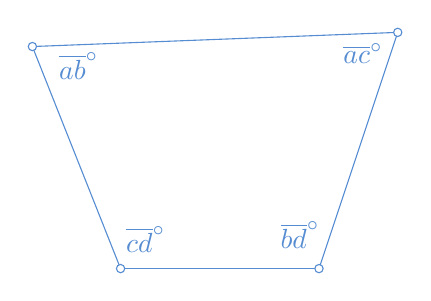
\begin{tikzpicture}[cackithi, node font= /small]
			\draw  (5.48,-1.)-- (8.,-1.);
			\draw  (8.,-1.)-- (9.,2.);
			\draw  (9.,2.)-- (4.36,1.82);
			\draw  (4.36,1.82)-- (5.48,-1.);
			\draw [fill=white] (5.48,-1.) circle (1.5pt);
			\draw (5.8,-0.63) node {$\overline{cd}^\circ$};
			\draw [fill=white] (8.,-1.) circle (1.5pt);
			\draw (7.76,-0.57) node {$\overline{bd}^\circ$};
			\draw [fill=white] (9.,2.) circle (1.5pt);
			\draw (8.56,1.73) node {$\overline{ac}^\circ$};
			\draw [fill=white] (4.36,1.82) circle (1.5pt);
			\draw (4.95,1.57) node {$\overline{ab}^\circ$};
		\end{tikzpicture}
		\vspace*{-10pt}
	\end{figure}
	\textit{Lời giải.} Do tổng bốn góc trong từ giác bằng $360^\circ,$ ta có
	\begin{align*}
		&10a + b + 10a + c + 10b + d + 10c + d \\
		= \,&20a+ 11b+11c+2d=360. \tag{$1$}
	\end{align*}
	Nhận xét rằng nếu $a\le 7$ thì  tổng trong $(1)$ không vượt quá $20\times 7 + 11\times 9 +11\times 9 + 2\times 9 =356.$ Do đó $a$ chỉ có thể nhận giá trị $8$ hoặc $9.$
	Do $b$ và $c$ có thể đổi vai trò cho nhau mà đáp án không thay đổi, ta có thể giả sử $b\ge c.$
	\vskip 0.1cm
	Trường hợp $I$: $a=8.$ Vì trong bốn góc phải có một góc không bé hơn $90^\circ$ nên $b=9.$ Phương trình $(1)$ trở thành $11c+2d=101$ và chỉ có nghiệm duy nhất là $c=9, d=1.$   
	\vskip 0.1cm
	Trường hợp $II$ $a=9$. Nếu $b\le 7$ thì tổng trong ($1$) không vượt quá $20\times 9 + 11\times 7 +11\times 7 + 2\times 9 = 352 < 360$ vô lý. Vậy $b = 8$ hoặc $b = 9$.
	\vskip 0.1cm
	Trường hợp $IIa$: $b=8.$ Phương trình $(1)$ trở thành $11c+2d=92.$ Do $c\le b=8,$ nên ta chỉ có nghiệm duy nhất $c=8, d=2.$
	\vskip 0.1cm
	Trường hợp $IIb$: $b=9.$ Phương trình $(1)$ trở thành $11c+2d=81.$ Dễ thấy phương trình chỉ có nghiệm duy nhất $c=7, d=2.$
	\vskip 0.1cm
	Tóm lại, có ba bộ bốn góc thỏa mãn bài toán: $\{\!89,\! 89,\! 91,\! 91\!\}\!,\! \{\!98,\! 98,\! 82,\! 82\!\}\!,\! \{\!99,\! 97,\! 92,\! 72\!\}.$
	\vskip 0.1cm
	{\bf\color{cackithi}OC$\pmb{32.}$} Cho hình ngũ giác đều $ABCDE$. Vẽ hai đường tròn: một có
	tâm $A$ và bán kính $AB$, và hình kia có tâm $B$ và bán kính $BA$. Gọi $X$ là giao điểm bên trong ngũ giác của hai đường tròn.
	Hỏi số đo của $\angle DEX$ bằng bao nhiêu?
	\vskip 0.1cm
	\textit{Lời giải.} Do $AX, BX, AB$ đều là bán kính của hai đường tròn nên chúng bằng nhau. Như vậy $ABX$ là tam giác đều. Vì mỗi góc trong ngũ giác đều  bằng $\frac{540^\circ}{5}=108^\circ,$ ta có $\angle EAX = 108^\circ - 60^\circ = 48^\circ.$
	\begin{figure}[H]
		\vspace*{-5pt}
		\centering
		\captionsetup{labelformat= empty, justification=centering}
		\definecolor{qqwuqq}{rgb}{0.,0.39215686274509803,0.}
		\definecolor{uuuuuu}{rgb}{0.26666666666666666,0.26666666666666666,0.26666666666666666}
		\definecolor{xdxdff}{rgb}{0.49019607843137253,0.49019607843137253,1.}
		\begin{tikzpicture}[cackithi,scale=1.2]
			\draw [shift={(1.3819660112501053,1.9021130325903073)},,color=qqwuqq,fill=qqwuqq,fill opacity=0.10000000149011612] (0,0) -- (-6.:0.6) arc (-6.:36.:0.6) -- cycle;
			\draw [] (2.,0.)-- (4.,0.);
			\draw [] (4.,0.)-- (4.618033988749895,1.9021130325903064);
			\draw [] (4.618033988749895,1.9021130325903064)-- (3.,3.077683537175253);
			\draw [] (3.,3.077683537175253)-- (1.3819660112501053,1.9021130325903073);
			\draw [] (1.3819660112501053,1.9021130325903073)-- (2.,0.);
			\draw [] (1.3819660112501053,1.9021130325903073)-- (3.,1.7320508075688772);
			\draw [] (3.,1.7320508075688772)-- (2.,0.);
			\draw [] (4.,0.)-- (3.,1.7320508075688772);
			\draw [shift={(4.,0.)},]  plot[domain=0.9272952180016115:3.4474715249946457,variable=\t]({1.*2.*cos(\t r)+0.*2.*sin(\t r)},{0.*2.*cos(\t r)+1.*2.*sin(\t r)});
			\draw [shift={(2.,0.)},]  plot[domain=-0.2992463156024767:2.2003262887940225,variable=\t]({1.*2.*cos(\t r)+0.*2.*sin(\t r)},{0.*2.*cos(\t r)+1.*2.*sin(\t r)});
			
				\draw [fill=white] (2.,0.) circle (1.5pt);
				\draw[] (1.7,-0.09) node {$A$};
				\draw [fill=white] (4.,0.) circle (1.5pt);
				\draw[] (4.3,-0.15) node {$B$};
				\draw [fill=white] (4.618033988749895,1.9021130325903064) circle (1.5pt);
				\draw[] (4.76,2.27) node {$C$};
				\draw [fill=white] (3.,3.077683537175253) circle (1.5pt);
				\draw[] (3.14,3.45) node {$D$};
				\draw [fill=white] (1.3819660112501053,1.9021130325903073) circle (1.5pt);
				\draw[] (1.2,2.29) node {$E$};
				\draw [fill=white] (3.,1.7320508075688772) circle (1.5pt);
				\draw[] (3.04,2.19) node {$X$};
		\end{tikzpicture}
		\vspace*{-10pt}
	\end{figure}
	Mặt khác, tam giác $AEX$ cân tại $A,$ nên $\angle AEX= \frac{180^\circ-48^\circ}{2}= 66^\circ.$ Ta nhận được $\angle DEX= 108^\circ - 66^\circ= 42^\circ.$
	\vskip 0.1cm
	{\bf\color{cackithi}OC$\pmb{33.}$} Seth làm $n$ viên xúc xắc giống hệt nhau bằng cách gấp $n$ bản giống như trong hình bên. Sau đó, anh ta xếp lần lượt các viên xúc xắc chồng lên nhau thành một hình tháp thẳng đứng.
	Biết rằng tổng số chấm ở mỗi một trong bốn mặt xung quanh của tháp xúc xắc đều là số lẻ. Hỏi các giá trị có thể của $n$ là bao nhiêu?
	\begin{figure}[H]
		\vspace*{-5pt}
		\centering
		\captionsetup{labelformat= empty, justification=centering}
		\hspace*{5pt}\includegraphics[height= 0.8\linewidth]{OC33}
		\includegraphics[height= 0.8\linewidth]{OC}
		\vspace*{-10pt}
	\end{figure}
	\textit{Lời giải.} Giả sử tổng số chấm trên $n$ ô của mặt đằng trước của tháp xúc xắc là $T$ và của mặt đằng sau là $S.$ Do tổng $2$ ô trên $2$ mặt đối diện của mỗi viên xúc xắc bằng $7,$ ta có $T+S=7n.$ Theo đầu bài thì cả $T$ và $S$ đều lẻ nên $n$ phải chẵn.
	\vskip 0.1cm
	Ta sẽ chứng minh rằng với mọi $n$ chẵn ta đều có thể xếp được một tháp xúc xắc như vậy. Trước tiên ta xếp $n$ viên xúc xắc theo hướng giống hệt nhau thành một tháp có mỗi mặt gồm toàn các số giống nhau. Sau đó ta xoay viên xúc xắc ở trên cùng đi sao cho các mặt trước, sau đổi chỗ cho nhau và các  mặt trái, phải cũng đổi chỗ cho nhau. 
	\vskip 0.1cm
	Bên dưới là hình minh họa trong trường hợp $n=4.$   Như vậy, tổng các chấm trên mỗi mặt của tháp có dạng $(n-1)a + 7-a=(n-2)a+7$ luôn là số lẻ. Do đó có thể xếp được tháp xúc xắc khi và chỉ khi $n$ chẵn.  
	\begin{figure}[H]
		\vspace*{-5pt}
		\centering
		\captionsetup{labelformat= empty, justification=centering}
		\includegraphics[width= 0.3\linewidth]{OC33b}
		\vspace*{-10pt}
	\end{figure}
	Trong phần cuối của chuyên mục kỳ này, chúng tôi sẽ giới thiệu với bạn đọc ba bài toán trong kỳ thi Olympic toán học trẻ  của Thổ Nhĩ Kỳ. Các bài toán này phù hợp với trình độ học sinh lớp $8-10$.
	\vskip 0.1cm
	{\bf\color{cackithi}OC$\pmb{40.}$} Cho $x, y, z$ là các số thực dương với $x\le 1.$ Chứng minh rằng
	\begin{align*}
		xy+y+2z \geq 4 \sqrt{xyz}.
	\end{align*}
	{\bf\color{cackithi}OC$\pmb{41.}$} Trong một trường có $101$ học sinh, mỗi học sinh có ít nhất một người bạn thân trong số các học sinh khác trong trường. Chứng minh rằng với mọi số nguyên $n, 1<n<101,$ ta có thể chọn một nhóm $n$ học sinh trong trường này sao cho mỗi học sinh được chọn có ít nhất một bạn thân trong số các học sinh khác được chọn. (Biết rằng nếu  $A$ là bạn thân của $B$ thì $B$ cũng là bạn thân của $A$).
	\vskip 0.1cm
	{\bf\color{cackithi} OC$\pmb{42.}$} Cho $m, n, a, k$ là các số nguyên dương và $k>1$ sao cho đẳng thức sau thỏa mãn 
	\begin{align*}
		5^m+63n+49=a^k.
	\end{align*} Tìm giá trị nhỏ nhất của $k$.
\end{multicols}

%	\newpage
%
%	\setcounter{figure}{0}
%	\thispagestyle{diendandayvahoctoannone}
\pagestyle{diendandayvahoctoan}
\everymath{\color{diendantoanhoc}}
\graphicspath{{../diendantoanhoc/pic/}}
\blfootnote{$^{1}$\color[named]{diendantoanhoc}THPT chuyên Lê Quý Đôn, Bình Định.}
\begingroup
\AddToShipoutPicture*{\put(0,616){\includegraphics[width=19.3cm]{../bannerdiendan}}}
\AddToShipoutPicture*{\put(124,525){\includegraphics[scale=1]{../tieude1.pdf}}}
\centering
\endgroup
\vspace*{192pt}

	\textit{\textbf{\color{diendantoanhoc}LTS.} Kỳ thi Bài giảng và bài viết về Toán học, lần thứ $2$, năm $2023$, do Tạp chí Pi tổ chức, với sự phối hợp của Hội Toán học, Viện Hàn lâm Khoa học và Công nghệ Việt Nam, là một diễn đàn dành cho độc giả của Pi và những người yêu Toán nói chung. Kỳ thi đã nhận được nhiều bài viết có chất lượng chuyên môn cao. Tạp chí Pi số này xin trân trọng giới thiệu cùng bạn đọc bài viết được trao giải Nhất trong hạng mục Chuyên đề Toán học.}
\begin{multicols}{2}
	Bài viết này trình bày về hai bổ đề liên quan đến mô hình hai đoạn thẳng và một vài ứng dụng trong việc tiếp cận, khai thác một số bài toán hình học phẳng.
	\vskip 0.1cm
	\textbf{\color{diendantoanhoc}$\pmb{1.}$ Bổ đề về hai đoạn thẳng} 
	\vskip 0.1cm
	Trong các bài toán hình học phẳng, chúng ta khá thường xuyên gặp tình huống có hai đoạn thẳng bằng nhau. Điều đó có thể gợi đến kết quả sau đây, mà chúng tôi tạm gọi là \textit{Bổ đề hai đoạn thẳng}.
	\vskip 0.1cm 
	\textbf{\color{diendantoanhoc}Bổ đề $\pmb{1.}$} Cho hai đoạn thẳng $AB$ và $A'B'$ trong mặt phẳng sao cho $AB$ không cùng phương với $A'B'$ và $AB=A'B'$. Khi đó tồn tại một phép quay biến $A$ thành $A'$ và $B$ thành $B'$. đồng thời cũng tồn tại một phép quay biến $A$ thành $B'$ và biến $B$ thành $A'$.
	\vskip 0.1cm
	Trước khi đi vào chứng minh, bạn đọc có thể nhận thấy rằng, bằng cách đổi vai trò của $A'$ và $B'$, ta suy ra tồn tại phép quay thứ hai biến $A$ thành $B'$ và  $B$ thành $A'$.
	\vskip 0.1cm
	\textit{Chứng minh.} Gọi $S$ là giao điểm của $AB$ và $A'B'$. Giả sử các đường trung trực của $AA'$ và $BB'$ cắt nhau tại $T$, dễ thấy hai tam giác $TAB$ và $TA'B'$ bằng nhau (c.c.c). Do đó $(BA,BT)=(B'A',B'T)\,\,\,(\bmod \pi)$, hay $(BS,BT)=(B'S,B'T)\,\,\,(\bmod \pi)$; suy ra bốn điểm $S,T,B,B'$ đồng viên. Tương tự thì bốn điểm $S,T,A,A'$ cũng đồng viên. Rõ ràng phép quay tâm $T$, góc quay $(TA,TA')=(TB,TB')$, biến  $A,B$ tương ứng thành $A',B'$. Trong trường hợp $AA'$ và $BB'$ song song thì từ giả thiết ta có hình thang cân $ABB'A'$. Lúc này $T$ trùng $S$ và ta cũng thu được kết quả như trên.
	\begin{figure}[H]
		\vspace*{-5pt}
		\centering
		\captionsetup{labelformat= empty, justification=centering}
		\includegraphics[scale=0.63]{1}
		\vspace*{-5pt}
	\end{figure}
	Chú ý rằng bổ đề trên dẫn đến kết quả sau đây.
	\vskip 0.1cm
	\textbf{\color{diendantoanhoc}Hệ quả.} Cho tam giác $ABC$ cố định, các điểm $M,N$ thay đổi lần lượt thuộc các cạnh $AB,AC$ sao cho $BM=CN$. Khi đó đường tròn $(AMN)$ luôn đi qua một điểm cố định khác $A$.
	\vskip 0.1cm
	\textit{Chứng minh.} Theo giả thiết ta có $BM=CN$ nên theo chứng minh của Bổ đề $1$ thì các đường tròn $(AMN)$ và $(ABC)$ cắt nhau tại $T$ (khác $A$) là giao điểm của các đường trung trực của các đoạn thẳng $MN$ và $BC$, tức là trung điểm cung $BC$ (chứa $A$) của đường tròn $(ABC)$. Mà $(ABC)$ cố định nên $T$ cố định. Vậy,  khi $M,N$ thay đổi thì đường tròn $(AMN)$ luôn đi qua một điểm cố định $T$ (khác $A$).	\vskip 0.1cm
	\vskip 0.1cm
	Bổ đề $1$ có một mở rộng tự nhiên như sau, trong đó giả thiết bằng nhau của các đoạn thẳng được bỏ đi và phép quay được thay bằng phép vị tự quay. Vì lý do này, chúng tôi cũng gọi kết quả sau là \textit{Bổ đề hai đoạn thẳng}.
	\vskip 0.1cm
	\textbf{\color{diendantoanhoc}Bổ đề $\pmb{2}$.} Cho hai đoạn thẳng $AB$ và $A'B'$ trong mặt phẳng sao cho hai đường thẳng $AB$ và $A'B'$ cắt nhau tại $P$. Khi đó tồn tại một phép vị tự quay biến $A$ thành $A'$ và $B$ thành $B'$. Ngoài ra, tâm của phép vị tự quay này là giao điểm thứ hai của hai đường tròn $(PAA')$ và $(PBB')$.
	\vskip 0.1cm
	Tương tự, bằng cách hoán đổi vai trò của các điểm, dễ thấy rằng cũng tồn tại một phép vị tự quay biến $A$ thành $B'$ và $B$ thành $A'$ (tâm của phép vị tự quay này là giao điểm thứ hai của các đường tròn $(PAB')$ và $(PBA')$).
	\begin{figure}[H]
		\vspace*{-5pt}
		\centering
		\captionsetup{labelformat= empty, justification=centering}
		\includegraphics[width=1\linewidth]{2}
		\vspace*{-20pt}
	\end{figure}
	\textit{Chứng minh.} Gọi $S$ là giao điểm thứ hai của các đường tròn $(PAA')$ và $(PBB')$. Ta có $(AS,AP)=(A'S,A'P) (\bmod  \pi)$, $(BS,BP)=(B'S,B'P)(\bmod  \pi)$ nên hai tam giác $SAB$ và $SA'B'$ đồng dạng. Như vậy, $S$ là tâm của phép vị tự quay biến đoạn $AB$ thành đoạn $A'B'$. 
	\vskip 0.1cm
	\textbf{\color{diendantoanhoc}Nhận xét.}  Ta có một số quan sát sau:
	\vskip 0.1cm
	$1)$ Nếu $S$ là tâm phép vị tự quay biến đoạn $AB$ thành đoạn $A'B'$ thì dễ thấy hai tam giác $SAB$ và $SA'B'$ đồng dạng nên $S$ cũng là tâm của phép vị tự quay biến đoạn $AA'$ thành đoạn $BB'$.
	\vskip 0.1cm 
	$2)$ Nếu hai đường tròn $(PAA')$, $(PBB')$  có tâm lần lượt là $O$, $O'$ thì $S$ cũng là tâm của phép vị tự quay biến đường tròn $(O)$ thành đường tròn $(O')$. Do đó ta có các tam giác $SAB,SA'B'$ và $SOO'$ đồng dạng.
	\vskip 0.1cm
	$3)$ Nếu $AA'$ cắt $BB'$ tại $Q$ thì các điểm $Q,S,A,B$ đồng viên và các điểm $Q,S,A',B'$ đồng viên. Điểm $S$ chính là điểm Miquel của tứ giác toàn phần xác định bởi $ABB'A'$.
	\begin{figure}[H]
		\vspace*{-5pt}
		\centering
		\captionsetup{labelformat= empty, justification=centering}
		\includegraphics[scale=0.75]{3}
		\vspace*{-10pt}
	\end{figure}
	$4)$ Với hai đoạn thẳng $AB,A'B'$ không cùng phương, luôn có hai phép vị tự quay biến đoạn thẳng này thành đoạn thẳng kia.
	\vskip 0.1cm
	$5)$ Trong trường hợp đặc biệt khi $AB=A'B'$, ta thu lại được kết quả của Bổ đề $1$ ở trên.
	\vskip 0.1cm
	\textbf{\color{diendantoanhoc}$2.$  Một số áp dụng}
	\vskip 0.1cm
	Bổ đề $1$ và $2$ tỏ ra khá hữu ích trong một số tình huống. Trong bài viết này, chúng tôi xin giới thiệu ứng dụng của chúng trong việc chứng minh các đoạn thẳng bằng nhau, chỉ ra một đường thẳng hoặc đường tròn đi qua điểm cố định và chứng minh một số đường tròn đồng quy.
	\vskip 0.1cm
	$\pmb{2.1.}$ \textbf{\color{diendantoanhoc}Chứng minh hai đoạn thẳng bằng nhau}
	\vskip 0.1cm
	Ví dụ đầu tiên được lấy từ một bài toán Vô địch Liên bang Nga năm $2006$.
	\vskip 0.1cm
	\textbf{\color{diendantoanhoc}Ví dụ $\pmb{1.}$} Cho tam giác $ABC$ nội tiếp đường tròn $(O)$. Hai điểm $M,N$ thay đổi trên $AB,AC$ sao cho $MN \parallel BC$, $MN$ cắt $(O)$ tại  $P,Q$ ($M$ nằm giữa $P$ và $N$). Gọi $J,K$ tương ứng là tâm đường tròn nội tiếp các tam giác $APB$, $AQC$ và $T$ là trung điểm của cung $BC$ chứa $A$ của đường tròn $(O)$. Chứng minh rằng $TJ=TK$.
	\begin{figure}[H]
		\vspace*{-5pt}
		\centering
		\captionsetup{labelformat= empty, justification=centering}
		\includegraphics[width= 0.9\linewidth]{4}
		\vspace*{-10pt}
	\end{figure}
	\textit{Phân tích:} Đề bài xuất hiện mô hình trung điểm cung $T$ và yêu cầu chứng minh $TJ=TK$. Đây là dấu hiệu khá rõ để ta vận dụng kết quả của Bổ đề $1$. Ta cần tìm ra hai đoạn thẳng bằng nhau có các đầu mút là $J$, $K$. Để ý tới giả thiết $MN$ song song với $BC$ và tính chất của tâm đường tròn nội tiếp là ta có thể tiếp cận được bài toán.
	\vskip 0.1cm
	\textit{Lời giải.} Giả sử $AJ,AK$ cắt $(ABC)$ tương ứng tại $X$, $Y$. Dễ thấy $X$, $Y$ tương ứng là trung điểm của các cung $PB$, $QC$ của đường tròn $(ABC)$. Theo một kết quả quen thuộc thì $XB=XP=XJ$ và  $YC=YQ=YK$. Mà $YC=XB$ nên $KY=XJ$. Áp dụng Bổ đề $1$ cho tam giác $AXY$, với hai điểm $J,K$ thỏa $XJ=YK$, ta suy ra đường trung trực của đoạn thẳng $JK$ đi qua trung điểm $T$ của cung $BC$ chứa $A$ của đường tròn $(ABC)$. Vậy $TJ=TK$.
	\vskip 0.1cm
	Ví dụ sau đây, được lấy từ kỳ thi Vô địch Liên bang Nga năm $2014$, cũng có thể được giải quyết bằng cách tương tự.
	\vskip 0.1cm
	\textbf{\color{diendantoanhoc}Ví dụ $\pmb{2.}$} Cho tam giác $ABC$ có $AB > AC$. Các điểm $M,N$ tương ứng nằm trên các cạnh $AC,AB$ sao cho $BN=CM$. Đường thẳng $MN$ cắt $BC$ tại $P$. Gọi $I$ là tâm đường tròn nội tiếp tam giác $PNB$, $J$ là tâm đường tròn bàng tiếp góc $P$ của tam giác $PMC$ và $T$ là trung điểm cung $BC$ chứa $A$. Chứng minh rằng  $TI=TJ$.
	\vskip 0.1cm
	\textit{Phân tích:} Đề bài tiếp tục xuất hiện mô hình trung điểm cung $T$ và hai đoạn thẳng $BN,CM$ bằng nhau nên cũng gợi ý đến việc vận dụng Bổ đề $1$. Tuy nhiên ý tưởng chứng minh $TI=TJ$ không giống như lời giải của ví dụ ở trên mà phải dùng đến một phép quay phù hợp. với tâm là trung điểm $T$ của cung $BC$ chứa $A$.
	\begin{figure}[H]
		\vspace*{-5pt}
		\centering
		\captionsetup{labelformat= empty, justification=centering}
		\includegraphics[width= 1\linewidth]{5}
		\vspace*{-10pt}
	\end{figure}
	\textit{Lời giải.} Theo Bổ đề $1$ thì tồn tại phép quay tâm $T$ biến $B,\,N$ lần lượt thành $C,\,M$, do đó tam giác $TNB$ biến thành tam giác $TMC$, đường tròn $(TNB)$ biến thành đường tròn $(TMC)$ suy ra $H$ biến thành $K$ ($H, K$ lần lượt là trung điểm cung $BN,CM$). Dễ chứng minh được $HB=HN=HI$; $KC=KM=KJ$. Mà $BN=CM$ nên ta có $HI=KJ$, từ đó suy ra được $TI=TJ$.
	\vskip 0.1cm
	\textbf{\color{diendantoanhoc}Ví dụ $\pmb{3.}$} Cho tứ giác lồi $ABCD$ có hai đường chéo $AC$ và $BD$ cắt nhau tại $P$. Gọi $I,J$ lần lượt là tâm các đường tròn $(PAD)$, $(PBC)$. Gọi $M,N,O$ lần lượt là trung điểm các đoạn thẳng $AC,BD,IJ$. Chứng minh $OM=ON$.
	\begin{figure}[H]
		\vspace*{-5pt}
		\centering
		\captionsetup{labelformat= empty, justification=centering}
		\includegraphics[width= 1\linewidth]{6}
		\vspace*{-15pt}
	\end{figure}
	\textit{Phân tích.} Bài toán xuất hiện mô hình hai đoạn thẳng cắt nhau: $AC$ và $BD$ cắt nhau tại $P$; ngoài ra, hai đường tròn $(PAD)$ và $(PBC)$ cắt nhau tại điểm thứ hai là $Q$ nên chúng là các dấu hiệu để áp dụng Bổ đề $2$ trong việc tiếp cận bài toán. Điểm $Q$ chính là tâm của phép vị tự quay mà ta quan tâm.
	\begin{figure}[H]
		\vspace*{-10pt}
		\centering
		\captionsetup{labelformat= empty, justification=centering}
		\includegraphics[width= 0.9\linewidth]{7}
		\vspace*{-10pt}
	\end{figure}
	\textit{Lời giải.} Áp dụng Bổ đề $2$ cho hai đoạn thẳng $AC$ và $BD$, do chúng cắt nhau tại $P$, ta biết rằng tồn tại phép vị tự quay $f$ với tâm $Q$ là giao điểm thứ hai (khác $P$) của các đường tròn $(PAD)$ và $(PBC)$. Phép vị tự quay $f$ biến $A$ thành $C$, biến $D$ thành $B$. Ngoài ra, ta biết rằng cũng tồn tại phép vị tự quay $g$ với tâm là $Q$ biến $A$ thành $D$, biến $C$ thành $B$; do đó đoạn $AC$  biến thành đoạn $DB$, dẫn đến $g$ biến $M$ thành $N$. Như vậy, các đường tròn $(PAD)$, $(PBC)$, $(PMN)$ cùng đi qua $Q$. Vì $f$ biến $A$ thành $C,D$ thành $B$ và $I$ thành $J$ nên các tam giác $QDB,QAC,QIJ$ đồng dạng với nhau. Từ đó suy ra các tam giác $QDN,QAM$ và $QIO$ đồng dạng. Do đó tồn tại một phép vị tự quay tâm $Q$ biến $D$ thành $N$, $A$ thành $M$ và $I$ thành $O$. Khi đó $O$ chính là tâm đường tròn $(QMN)$ nên ta có $OM=ON$.
	\vskip 0.1cm
	\textit{Nhận xét.} Kết luận của bài toán vẫn còn đúng khi $A,B,C,D$ là bốn điểm bất kỳ sao cho $AC$ và $BD$ cắt nhau. 
	\vskip 0.1cm
	$\pmb{2.2.}$ \textbf{\color{diendantoanhoc}Chứng minh tính thẳng hàng, đồng quy}
	\vskip 0.1cm
	Bài toán sau đây, được lấy từ các bài toán đề nghị thi Toán quốc tế năm $2006$, minh họa một ứng dụng khác của các Bổ đề $1$ và $2$.
	\vskip 0.1cm
	\textbf{\color{diendantoanhoc}Ví dụ $\pmb{4.}$} Cho ngũ giác lồi $ABCDE$ thỏa mãn $\angle BAC = \angle CAD = \angle DAE,$ $\angle CBA = \angle DCA =\angle EDA$. Gọi $P$ là giao điểm của $BD$ và $CE$. Chứng minh rằng $AP$ đi qua trung điểm của $CD$. 
	\begin{figure}[H]
		\vspace*{-5pt}
		\centering
		\captionsetup{labelformat= empty, justification=centering}
		\includegraphics[width= 1\linewidth]{9}
		\vspace*{-15pt}
	\end{figure}
	\textit{Phân tích.} Trong bài toán này, dấu hiệu nhận biết việc áp dụng Bổ đề $2$ là hai đoạn thẳng $BD$ và $CE$ cắt nhau tại $P$ và các tam giác $ABC$, $ADE$ có chung đỉnh $A$ và đồng dạng với nhau. Khi đó, giao điểm thứ hai của các đường tròn $(PBC)$ và $(PDE)$ chính là tâm của phép vị tự quay. 
	\vskip 0.1cm
	\textit{Lời giải $1$.} Một mặt, theo giả thiết thì hai tam giác $ABC$ và $ADE$ đồng dạng nên có một phép vị tự quay tâm $A$ biến $B$ thành $C$, biến $D$ thành $E$, và đoạn thẳng $BD$ biến thành đoạn thẳng $CE$. Áp dụng Bổ đề $2$ cho hai đoạn thẳng $BD$ và $CE$ ta thấy rằng phép vị tự quay này có tâm là giao điểm thứ hai của các đường tròn $(PBC)$ và $(PDE)$, vì thế $A$ là giao điểm thứ hai của $(PBC)$ và $(PDE)$.
	\vskip 0.1cm
	Mặt khác, vì các tam giác $ABC,ACD,ADE$ đồng dạng (g.g) nên ta có $\angle ABC = \angle ACD, \angle ADC = \angle AED$. Do đó $CD$ là tiếp tuyến chung của hai đường tròn $(PBC)$ và $(PDE)$. Mà hai đường tròn này có trục đẳng phương là $AP$ nên nó chia đôi $CD$.
	\vskip 0.1cm
	Để so sánh với lời giải sử dụng Bổ đề 1 trên đây, chúng tôi trình bày một lời giải thứ hai.
	\textit{Lời giải $2$.} Gọi $X$ là giao điểm của $AC$ và $BD$, $Y$ là giao điểm của $AD$ và $CE$. Theo \textit{Lời giải $1$}, tồn tại phép vị tự quay $f$ tâm $A$ biến $B,\,C,\,D$ tương ứng thành $C,\,D,\,E$. Vì thế, $f$ biến các đoạn thẳng $AC$ và $BD$ tương ứng thành $AD$ và $CE$. Suy ra giao điểm của $AC$ và $BD$ biến thành giao điểm của $AD$ và $CE$, tức là $f$ biến $X$ thành $Y$.
	\begin{figure}[H]
		\vspace*{-5pt}
		\centering
		\captionsetup{labelformat= empty, justification=centering}
		\includegraphics[width= 1\linewidth]{10}
		\vspace*{-15pt}
	\end{figure}
	Từ đó ta có
	\begin{align*}
		\dfrac{XA}{XC} = \dfrac{YA}{YD}. \tag{$*$}
	\end{align*}
	Gọi $I$ là giao điểm của $AP$ với $CD$ và áp dụng định lý Ceva cho tam giác $ACD$ với điểm đồng quy $P$, ta có
	\begin{align*}
		\frac{XA}{XC}\cdot \frac{IC}{ID}\cdot\frac{YD}{YA} = 1.
	\end{align*}
	Từ đó, kết hợp ($*$), ta suy ra $IC=ID$.
	\vskip 0.1cm
	\textit{Nhận xét.}  Lời giải $2$ không dùng đến Bổ đề về hai đoạn thẳng mà dùng đến kết quả của phép vị tự quay. Việc phát hiện ra hệ thức $(*)$ là điều không hề dễ. Theo quan sát trong thực tế dạy học của tác giả, rất ít học sinh nghĩ ra  lời giải theo hướng này. Mặt khác, sau khi biết về bổ đề hai đoạn thẳng thì đa số học sinh dễ dàng phát hiện ra dấu hiệu và áp dụng vào bài toán một cách dễ dàng.
	\vskip 0.1cm
	Bài toán sau đây được lấy từ một kỳ thi Vô địch Liên bang Nga.
	\vskip 0.1cm
	\textbf{\color{diendantoanhoc}Ví dụ $\pmb{5.}$} Cho tam giác nhọn $ABC$. Gọi $A_1$, $B_1$, $C_1$ tương ứng là tiếp điểm của các đường tròn bàng tiếp góc $A$ với $BC$, góc $B$ với $CA$, góc $C$ với $AB$. Các đường tròn $(AB_1C_1)$, $(BC_1A_1)$, $(CA_1B_1)$ cắt lại $(ABC)$ tại $M,N,P$. Gọi $D,E,F$ là các tiếp điểm của đường tròn nội tiếp với $BC,CA,AB$. Chứng minh rằng $MD,NE,PF$ đồng quy.
	\begin{figure}[H]
		\vspace*{-5pt}
		\centering
		\captionsetup{labelformat= empty, justification=centering}
		\includegraphics[width= 0.9\linewidth]{11}
		\vspace*{-10pt}
	\end{figure}
	\textit{Phân tích.} Bằng hình vẽ ta dễ phát hiện ra rằng $M,N,P$ tương ứng là các trung điểm cung $BC,CA,AB$ của đường tròn $(ABC)$ và đây là dấu hiệu để ta nghĩ đến cách tiếp cận bài toán dựa vào Bổ đề $1$. Như vậy ta phải tìm những cặp đoạn thẳng bằng nhau, tuy nhiên điều này không quá khó khi dựa vào tính chất tiếp tuyến và tiếp điểm của các đường tròn nội tiếp, bàng tiếp.
	\vskip 0.1cm
	\textit{Lời giải.} Dễ thấy $CB_1 =AE=AF=BC_1$. Áp dụng Bổ đề $1$ ta có $M$ là trung điểm cung $BC$ chứa $A$ của $(ABC)$; tương tự với $N,P.$ Ta dễ thấy rằng hai tam giác $DEF$ và $MNP$ có các cặp cạnh tương ứng song song (chẳng hạn $NP$ và $EF$ cùng vuông góc với phân giác trong góc $A$). Vì vậy tồn tại một phép vị tự biến $D,E,F$ tương ứng thành $M,N,P$. Vậy $MD,NE,PF$ đồng quy tại tâm vị tự của hai tam giác trên. 
	\vskip 0.1cm
	Bài toán sau đây được trích từ kỳ thi chọn học sinh giỏi quốc gia năm 2017 của Việt Nam.
	\textbf{\color{diendantoanhoc}Ví dụ 6.} Cho tam giác $ABC$ nhọn, không cân, nội tiếp đường tròn $(O)$. Các đường cao $BE$, $CF$ cắt nhau tại $H$, $AH$ cắt $(O)$ tại $D$  (khác $A$). Các đường thẳng $DE,DF$ cắt lại $(O)$ tương ứng  $P,Q$ (khác $D$). Đường tròn $(AEF)$ cắt $(O)$ và $AO$ tương ứng tại $R,S$ (khác $A$). Chứng minh rằng $BP$, $CQ$ và $RS$ đồng quy.
	\vskip 0.1cm
	Chúng ta sẽ giới thiệu hai lời giải, một lời giải sử dụng phép biến đổi góc và lời giải còn lại sử dụng Bổ đề $2$.
	\vskip 0.1cm
	\textit{Lời giải $1$.} Gọi $X$ là trung điểm của $EF$ và $K$ là giao điểm của $AD$ và $BC$. Dễ thấy hai tam giác $BFE$ và $KHE$ đồng dạng (g.g). Gọi $T$ là trung điểm của $HE$. Khi đó, do $X$ là trung điểm $FE$ nên ta suy ra hai tam giác $BFX$ và $KHT$ đồng dạng. Vì $K$ là trung điểm $DH$ nên tam giác $KHT$ và tam giác $DHE$ đồng dạng, dẫn đến các tam giác $BFX$ và $DHE$ là đồng dạng. Suy ra  $\angle{FBX}= \angle{HDE}$, kết hợp với  $\angle{HDE}=\angle{ADP} = \angle{ABP}=\angle{FBP} $ ta được  $\angle{FBX}= \angle{FBP}.$ Từ đây ta có $B,P,X$ thẳng hàng. Tương tự ta có $C,X,Q$ thẳng hàng.
	\begin{figure}[H]
		\vspace*{-10pt}
		\centering
		\captionsetup{labelformat= empty, justification=centering}
		\includegraphics[width= 0.9\linewidth]{12}
		\vspace*{-15pt}
	\end{figure}
	Kẻ đường kính $AL$ của $(O)$. Dễ thấy $SH$ đi qua $L$ và do tứ giác $HBLC$ là hình bình hành nên $HL$ đi qua trung điểm $M$ của $BC$. Dễ thấy hai tam giác $SEC$ và $SFB$ đồng dạng (g.g) nên hai tam giác $SEF$ và $SCB$ đồng dạng (c.g.c). Mà hai tam giác này có các trung tuyến tương ứng là $SX$ và $SM$ nên ta suy ra $\angle FSX =  \angle BSM$. Tương tự, do hai tam giác $SFB$ và $SRL$ đồng dạng (g.g) nên hai tam giác $SFR$ và $SBL$ đồng dạng (c.g.c), dẫn đến  $\angle FSR=\angle BSL=\angle BSM=\angle FSX$. Từ đó suy ra $S,X,R$ thẳng hàng. Vậy, $SR,BP,CQ$ đồng quy tại trung điểm $X$ của $EF$.
	\vskip 0.1cm
	\textit{Lời giải $2$.} Gọi $X$ là trung điểm của $EF$. Tương tự như \textit{Lời giải $1$}, ta cũng chứng minh được $BP$ và $CQ$ đi qua $X$. Ta cần chứng minh $SR$ cũng đi qua $X$. Kẻ đường kính $AL$. Áp dụng Bổ đề $2$ cho hai đoạn thẳng $BF$ và $CE$ (và để ý rằng chúng cắt nhau tại $A$) ta suy ra $S$ là tâm của phép vị tự quay $f$ biến đoạn $FE$ thành đoạn $BC$ và biến $X$ biến thành $M$. Từ đó $f$ biến $(AEF)$ thành $(ABC)$. Kết hợp với việc $A,R,L$ thẳng hàng, ta suy ra $f$ biến $R$ thành $L$. Các điểm $S,L,M$ tương ứng biến thành $S,R,X$. Mà  $S,L,M$ thẳng hàng nên $S,R,X$ thẳng hàng. Vậy, $SR,BP,CQ$ đồng quy tại $X$.
	\vskip 0.1cm
	\textit{Nhận xét.} Ở lời giải thứ nhất, để chứng minh $SR$ đi qua $X$, ta đã sử dụng phép biến đổi góc dựa vào việc tìm ra những cặp tam giác đồng dạng khá phức tạp. Tuy nhiên ở lời giải thứ hai thì việc áp dụng Bổ đề $2$ cho ta cách tiếp cận dễ dàng hơn nhiều. Dấu hiệu nhận biết ở đây là việc hai đường tròn $(O)$ và $(AEF)$ cắt nhau tại $ A,S$ và có $BF$ cắt $CE$ tại $A$.
	\vskip 0.1cm 
	$\pmb{2.3.}$ \textbf{\color{diendantoanhoc} Chứng minh đường thẳng hoặc đường tròn luôn qua điểm cố định}
	\vskip 0.1cm
	Bài toán sau đây được lấy từ đề thi Toán quốc tế (IMO) năm $2005$.
	\vskip 0.1cm
	\textbf{\color{diendantoanhoc}Ví dụ $\pmb{7}$.} Cho $ABCD$ là tứ giác lồi có $AD=BC$ và $AD,BC$ không song song. Gọi $E,F$ tương ứng  là các điểm trên $BC,AD$ sao cho $BE=DF$. Các đường thẳng  $AC$ và $BD$ cắt nhau tại $P$, các đường thẳng $BD$ và $EF$ cắt nhau tại $Q$, các đường thẳng $EF$ và $AC$ cắt nhau tại $R$. Chứng minh rằng, khi $E$ và $F$ thay đổi, đường tròn $(PQR)$ đi qua một điểm cố định khác $P$.
	\begin{figure}[H]
		\vspace*{-5pt}
		\centering
		\captionsetup{labelformat= empty, justification=centering}
		\includegraphics[width= 1.02\linewidth]{14}
		\vspace*{-15pt}
	\end{figure}
	\textit{Lời giải $1$.} Theo Bổ đề $1$, áp dụng cho hai đoạn thẳng $AD=BC$ có $AC$ cắt $BD$ tại $P$,  ta có giao điểm $S$ của hai đường tròn $(PAD)$ và $(PBC)$ là tâm phép quay (góc  $ \angle BSD$) biến $A$ thành $C$ và biến $D$ thành $B$, do đó ta có các tam giác cân $SAC,SBD$ đồng dạng. Vì $FD/FA=EB/EC$ nên phép quay này biến $F$ thành $E$, do đó ta có $SF=SE$ và $(FS, FR)=(FS, FE)=(AS, AC)=(AS, AR)\,\,\,(\bmod \pi)$. Do đó $A,S, R, F$ đồng viên. Tương tự, $B, E, Q, S$ đồng viên và $D, F, S, Q$ đồng viên. Từ đó $(RS, RP)=(FS, FA)=(FS, FD)=(QS, QP)\,\,\,(\bmod \pi)$. Suy ra $(PQR)$ đi qua điểm $S$ cố định.
	\vskip 0.1cm
	\textit{Lời giải $2$.} Theo Bổ đề $2$, tồn tại phép vị tự quay $f$ biến $A$ thành $C$ và biến $D$ thành $B$. Khi đó $f$ biến $ F$ thành $E$ (do $FD/FA=EB/EC$), và đoạn $DF$ biến thành đoạn $BE$. Do đó hai tứ giác $ACBD$ và $EFDB$ có chung điểm Miquel. Tâm của phép vị tự quay $f$ là giao điểm thứ hai $S$ của hai đường tròn $(PAD)$ và $(PCB)$, cũng là điểm Miquel chung của các tứ giác toàn phần $ACBD$ và $EFDB$. Do đó $S$ thuộc các đường tròn $(QEB)$ và $(QFD)$. Dễ thấy $S$ cũng là điểm Miquel chung của các tứ giác toàn phần $DFRP$ và $CEQP$, do đó $S$ thuộc $(PQR)$. Vì các đường tròn $(PAD)$ và $(PBC)$ cố định nên $S$ cố định. Vậy, đường tròn $(PQR)$ luôn đi qua điểm $S$ cố định. 
	\begin{figure}[H]
%		\vspace*{-5pt}
		\centering
		\captionsetup{labelformat= empty, justification=centering}
		\includegraphics[width= 1\linewidth]{15}
		\vspace*{-10pt}
	\end{figure}
	\textit{Nhận xét.} $1)$ Điều thú vị là đối với bài toán này lại, chúng ta vừa có thể áp dụng Bổ đề $1$, vừa có thể áp dụng Bổ đề $2$ để giải. Điều đó cho thấy sự đa dạng và phạm vi vận dụng rộng rãi của hai bổ đề mà chúng ta đã đề cập. Trong bài toán trên, dấu hiệu để phát hiện và tiếp cận theo hướng Bổ đề $1$  là sự xuất hiện của hai đoạn thẳng bằng nhau. Mặt khác, dấu hiệu để tiếp cận và vận dụng bổ đề $2$ là có mô hình hai đoạn thẳng $AC$ và $BD$ cắt nhau tại $P$, đồng thời hai đường tròn $(PAD)$, $(PBC)$ cắt nhau tại $P$ và $S$. Hơn nữa, bài toán cũng xuất hiện hai điểm $E,F$ chia các đoạn thẳng với tỷ lệ bằng nhau nên ta nghĩ đến phép vị tự quay biến $F$ thành $E$; tâm của phép vị tự quay chính là điểm $S$.
	\vskip 0.1cm
	$2)$ Nếu thay giả thiết tứ giác $ABCD$ lồi thành bốn điểm $A, B, C, D$ bất kỳ ta vẫn thu được kết luận tương tự và các lời giải trên vẫn còn đúng.
	\vskip 0.1cm
	\textbf{\color{diendantoanhoc}Ví dụ $\pmb{8.}$} Cho tam giác $ABC$ nội tiếp đường tròn $(O)$ cố định với $B,C$ là các điểm cố định và điểm $A$ thay đổi trên $(O)$. Các đường cao $AD,BE,CF$ đồng quy tại $H,BO$ và $CO$ tương ứng cắt $DF,DE$ tại $K,L,KL$ cắt $EF$ tại $P$. Chứng minh rằng đường tròn $(PEL)$ luôn qua một điểm cố định.
	\vskip 0.1cm
	\textit{Phân tích.} Để ý rằng các điểm $E,F,K,L$ cùng với $P,D$ lập thành một tứ giác toàn phần, vì vậy khi xét điểm cố định mà đường tròn $(EPL)$ đi qua, ta quan tâm đến điểm Miquel của tứ giác toàn phần $EFKLPD$. Lại có $(EFD)$ chính là đường tròn Euler của tam giác $ABC$, và trung điểm $M$ của $BC$ là trung điểm cung $EF$ chứa $D$ của đường tròn này. Như vậy, ta chỉ cần chứng minh $M$ chính là điểm Miquel của tứ giác toàn phần đã nêu. Để chỉ ra điều đó, ta đưa về mô hình hai đoạn thẳng bằng nhau và áp dụng Bổ đề $1$. Từ đó ta có thể tiếp cận bài toán như sau.
	\begin{figure}[H]
		\vspace*{-5pt}
		\centering
		\captionsetup{labelformat= empty, justification=centering}
		\includegraphics[width= 1\linewidth]{16}
		\vspace*{-10pt}
	\end{figure}
	\textit{Lời giải.} Vì $BH, BO$ đẳng giác trong góc $B$ nên $BO$ vuông góc với $FD$. Tương tự, $CO$ vuông góc với $ED$. Để ý rằng $B,C$ tương ứng là tâm các đường tròn bàng tiếp góc $E,F$ của tam giác $DEF$ nên ta dễ chứng minh được $KF=LE$. Gọi $M$ là trung điểm $BC$. Dễ thấy $ME=MF$ nên $M$ là trung điểm của cung $FE$ chứa $D$ của đường tròn $(FDE)$, đường tròn Euler của tam giác $ABC$. Do đó theo Bổ đề $1$ thì $M$ là điểm Miquel của tứ giác toàn phần $EFKLDP$. Vì thế đường tròn $(LEP)$ luôn qua điểm $M$ cố định khi $A$ di động trên $O$.
	\vskip 0.1cm
	Bài toán sau đây do tác giả Trần Quang Hùng đề xuất.
	\vskip 0.1cm
	\textbf{\color{diendantoanhoc}Ví dụ $\pmb{9.}$} Cho tam giác $ABC$. Các điểm $E,F$ tương ứng thay đổi trên $AC,AB$ sao cho $CE=BF$. Chứng minh rằng đường thẳng Euler của tam giác $AEF$ luôn đi qua một điểm cố định.
	\vskip 0.1cm
	\textit{Phân tích.} Rõ ràng bài toán này có mô hình hai đoạn thẳng bằng nhau là $CE=BF$ nên ta có thể vận dụng Bổ đề $1$ để tiếp cận. Theo Bổ đề $1$ thì hai đường tròn $(AEF)$ và $(ABC)$ cắt nhau tại trung điểm cung của mỗi đường tròn, từ đó ta có thêm thông tin để giải bài toán.
	\vskip 0.1cm
	\textit{Lời giải.} Gọi $ G,L$ tương ứng là trọng tâm các tam giác $ABC,AEF$. Gọi $(O)$ và $(K)$ tương ứng là các đường tròn ngoại tiếp các tam giác $ABC, AEF$. Khi đó $LK,GO$ tương ứng là đường thẳng Euler của các tam giác $AEF,ABC$. Gọi giao điểm của $LK$ và $ GO$ là $R$. Ta sẽ chứng minh $R$ là một điểm cố định. Thật vậy, theo Bổ đề $1$ thì $(O)$ và $(K)$ cắt nhau tại $T$ trên các đường trung trực $EF,BC$. Gọi $ M,N$ tương ứng là trung điểm của các đoạn thẳng $BC,EF$. Ta thấy rằng các tam giác cân $TEF,TBC$ đồng dạng, do đó ta suy ra được $\dfrac{TK}{TN} = \dfrac{KO}{MN} = \dfrac{TO}{TM}$, là tỷ số không đổi.
	\begin{figure}[H]
		\vspace*{-5pt}
		\centering
		\captionsetup{labelformat= empty, justification=centering}
		\includegraphics[width= 1\linewidth]{17}
		\vspace*{-10pt}
	\end{figure}
	Suy ra $MN\parallel KO$. Ta lại có $\dfrac{GL}{MN} = \dfrac{2}{3}$  và $GL\parallel MN$, do đó $GL\parallel KO$ và
	\begin{align*}
		\dfrac{GL}{KO} = \dfrac{GL}{MN}\cdot \frac{MN}{KO} = \dfrac{2}{3} \cdot \dfrac{TM}{TO}.
	\end{align*}
	Từ đó, tỷ số $\dfrac{RG}{RO} = \dfrac{GL}{KO}$ là không đổi, do đó điểm $R$ là cố định. Vậy $KL$ luôn đi qua điểm $R$ cố định.
	\vskip 0.1cm
	$\pmb{2.4.}$ \textbf{\color{diendantoanhoc}Chứng minh nhiều đường tròn đồng quy}
	\vskip 0.1cm
	Bài toán sau đây xuất hiện trong đề thi Olympic Toán quốc gia của Mỹ năm $2006$.
	\vskip 0.1cm
	\textbf{\color{diendantoanhoc}Ví dụ $\pmb{10.}$}  Cho tứ giác lồi $ABCD$ có các cặp cạnh đối không song song và $E,F$ lần lượt là các điểm trên các cạnh $AD$ và $BC$ sao cho  $\dfrac{AE}{ED} = \dfrac{BF}{FC}$, $EF$ cắt $AB,CD$ lần lượt tại $S,T$. Chứng minh các đường tròn $(SAE)$, $(SBF)$, $(TCF)$, $(TDE)$ cùng đi qua một điểm.
	\vskip 0.1cm
	\textit{Phân tích.} Đề bài cho tứ giác toàn phần $ABCD$ và các điểm $E,F$ lần lượt chia các đoạn $AD,BC$ theo cùng tỷ số nên ta có thể liên tưởng đến mô hình hai đoạn thẳng. Hơn nữa, yêu cầu bài toán là chứng minh các đường tròn đồng quy nên ta có thể nghĩ đến điểm Miquel của tứ giác toàn phần, cũng chính là tâm của phép vị tự quay trong Bổ đề $2$.
	\begin{figure}[H]
		\vspace*{-5pt}
		\centering
		\captionsetup{labelformat= empty, justification=centering}
		\includegraphics[width= 1\linewidth]{18}
		\vspace*{-10pt}
	\end{figure}
	\textit{Lời giải.} Gọi $M$ là tâm của phép vị tự quay $f$ biến $A$ thành $B$, biến $D$ thành $C$, do đó biến $AD$ thành $BC$. Vì các điểm $E,F$ chia các đoạn thẳng này theo cùng tỷ số nên phép vị tự quay này cũng biến $E$ thành $F$. Do đó $f$ biến $AE$ thành $BF$ và biến $ED$ thành $FC$. Như vậy, tâm $M$ là điểm Miquel chung của các tứ giác toàn phần $ABFE$ và $EFCD$ (cũng như tứ giác $ABCD$). Vậy, các đường tròn $(SAE)$, $(SBF)$, $(TCF)$, $(TDE)$ cùng đi qua điểm Miquel $M$.
	\begin{figure}[H]
%		\vspace*{-5pt}
		\centering
		\captionsetup{labelformat= empty, justification=centering}
		\includegraphics[width= 1\linewidth]{19}
		\vspace*{-10pt}
	\end{figure}
	\textit{Nhận xét:} Nếu thay giả thiết tứ giác $ABCD$ lồi bởi bốn điểm $A,B,C,D$ bất kỳ thì ta cũng thu được kết quả tương tự.
	\vskip 0.1cm
	$\pmb{2.5.}$ \textbf{\color{diendantoanhoc}Một số bài tập}
	\vskip 0.1cm
	Để kết thúc bài viết, chúng tôi xin mời độc giả thử sức mình với một số bài toán mà lời giải có thể sử dụng các Bổ đề $1$ và $2$.
	\vskip 0.1cm
	\textbf{\color{diendantoanhoc}Bài $\pmb{1}$ (Chọn đội tuyển Mỹ năm $\pmb{2007}$).} Hai đường tròn $(O)$ và $(O')$ cắt nhau tại $P,Q$.  Qua $P$ vẽ hai cát tuyến $PAB$ và $PCD$ sao cho $A,C$ thuộc $(O)$ và $B,D$ thuộc $(O')$. Tia $BD$ cắt đoạn $AC$ tại $X$. Lấy điểm $Y$ thuộc $(O)$ và $Z$ thuộc $(O')$ sao cho $PY\parallel BD,PZ\parallel AC$. Chứng minh $Q,X,Y,Z$ thẳng hàng.
	\vskip 0.1cm
	\textbf{\color{diendantoanhoc}Bài $\pmb{2}$.} Cho tam giác $ABC$, các điểm $E,F$ di chuyển trên $AC,AB$ sao cho $CE=BF$. Chứng minh rằng tâm đường tròn Euler của tam giác $AEF$ luôn thuộc một đường thẳng cố định khi $E,F$ di chuyển.
	\vskip 0.1cm
	\textbf{\color{diendantoanhoc}Bài $\pmb{3}$.} Cho tam giác $ABC$ có trung tuyến $AM$. Gọi $I,J$ lần lượt là tâm các đường tròn $(AMB),(AMC),O$ là tâm đường tròn $(ABC)$. Chứng minh $AO$ là đường đối trung của tam giác $AIJ$.
	\vskip 0.1cm
	\textbf{\color{diendantoanhoc}Bài $\pmb{4}$ (Olympic Iran $\pmb{1997}$).} Cho tam giác ABC nội tiếp đường tròn $(O)$. Điểm $P$ di chuyển trên cung $BC$ không chứa $A$, gọi $I,J$ lần lượt là tâm nội tiếp các tam giác $APB,APC$. Chứng minh đường tròn $(PIJ)$ luôn đi qua một điểm cố định.
	\vskip 0.1cm
	\textbf{\color{diendantoanhoc}Bài $\pmb{5}$.} Cho hai đường tròn $(O)$ và $(O')$ cắt nhau  tại $A,B$. Một cát tuyến thay đổi qua $A$ cắt $(O),(O')$ lần lượt tại $D,E$. Tiếp tuyến của $(O)$ tại $D$ và tiếp tuyến của $(O')$ tại $E$ cắt nhau tại $P$. Chứng minh rằng trung trực của đoạn $BP$ luôn tiếp xúc với một đường tròn cố định.
	\vskip 0.1cm
	\textbf{\color{diendantoanhoc}Bài $\pmb{6}$ (Olympic Canada $\pmb{2013}$).} Cho tam giác $ABC$ vuông tại $C$ có trọng tâm $G$, gọi $P$ là điểm trên $AG$ sao cho  $\angle CPA = \angle CAB$, $Q$ là điểm trên $BG$ sao cho  $\angle CQB = \angle ABC$. Chứng minh rằng các đường tròn $(AQG)$ và $(BPG)$ cắt nhau tại một điểm thuộc cạnh $AB$.
	\vskip 0.1cm
	\textbf{\color{diendantoanhoc}Bài $\pmb{7}$.} Cho tam giác $ABC$ nhọn có trực tâm $H$ và nội tiếp đường tròn $(O)$. Trung trực $AH$ cắt $AB,AC$ lần lượt tại $D,E$. Chứng minh rằng $OA$ là phân giác của góc  $\angle DOE$.
	\vskip 0.1cm
	\textbf{\color{diendantoanhoc}Bài $\pmb{8}$ (Olympic Trung Quốc $\pmb{1992}$).} Cho tứ giác lồi $ABCD$ nội tiếp đường tròn $(O),AC$ cắt $BD$ tại $P$, các đường tròn $(PAB)$ và $(PCD)$ cắt nhau tại $Q$ khác $P$ và $O$. Chứng minh $QO$ vuông góc với $QP$.
	\vskip 0.1cm
	\textbf{\color{diendantoanhoc}Bài $\pmb{9}$ (Olympic Toán quốc tế $\pmb{2004}$).} Cho tứ giác lồi $ABCD$, đường chéo $BD$ không là phân giác các góc  $\angle ABC, \angle CDA$. Điểm $P$ nằm trong tứ giác sao cho  $\angle PBC = \angle DBA, \angle DBC = \angle BDA$. Chứng minh tứ giác $ABCD$ nội tiếp được khi và chỉ khi $PA=PC$.
	\vskip 0.1cm
	\textbf{\color{diendantoanhoc}Bài $\pmb{10}$.} Cho tam giác $ABC$ nội tiếp đường tròn $(O),N$ là trung điểm cung $BC$ chứa $A$ của $(O), M$ là một điểm bất kỳ trên trung trực đoạn $BC$. Gọi $I,J$ lần lượt là tâm đường tròn bàng tiếp góc $A$ của các tam giác $ABM,ACM$. Chứng minh $I,J,A,N$ đồng viên.
	\vskip 0.1cm
	\textbf{\color{diendantoanhoc}Tài liệu tham khảo}
	\vskip 0.1cm
	[$1$] Lê Bá Khánh Trình, \textit{Hình học tĩnh và động}, tạp chí Pi, số $8$, tháng $8/2019$. 
	\vskip 0.1cm
	[$2$] Trần Quang Hùng. \textit{Ứng dụng một số bổ quen thuộc vào các bài toán hình học thi Olympic}.
	\vskip 0.1cm
	[$3$] Nguyễn Minh Hà, Nguyễn Xuân Bình, \textit{Bài tập nâng cao và một số chuyên đề Hình học $10$}, NXB Giáo dục, $2008$.
	\vskip 0.1cm
	[$4$] Nguyễn Văn Ban, Hoàng Chúng, \textit{Hình học của tam giác}, NXB Giáo dục.
	\vskip 0.1cm
	[$5$] V.V. Praxolov, \textit{Các bài toán về hình học phẳng, Tập II}, NXB Hải Phòng, $2002$.
	\vskip 0.1cm
	[$6$] Johnson, A. R, \textit{Advanced Euclidean Geometry}, Publications, Inc, Mineola, New York, $2007$.
\end{multicols}
\vspace*{-10pt}
\rule{1\linewidth}{0.1pt}
\blfootnote{$^{1}$\color[named]{diendantoanhoc}Tòa soạn Hà Nội, Báo Thanh Niên.}
\begingroup
\AddToShipoutPicture*{\put(114,235){\includegraphics[scale=1]{../tieude.pdf}}}
\centering
\endgroup
\vspace*{80pt}

\textit{Với những ai quan tâm kỳ thi Bài giảng và bài viết về Toán học mang tên Hoàng Tụy, không chỉ là xem các thí sinh thuyết trình bài giảng, mà hơn thế, được nghe các thầy giám khảo chia sẻ quan điểm về dạy toán.}

\begin{multicols}{2}
	Theo nhận định của nhiều người theo dõi, điều lôi cuốn người xem nhất ở vòng chung khảo kỳ thi Bài giảng và bài viết về Toán học, mang tên Hoàng Tụy, là phần nhận xét của các thành viên hội đồng giám khảo. Nội dung các nhận xét này không chỉ đơn giản chỉ là những lời khen chê. Quan trọng hơn, đó là những chia sẻ về quan điểm dạy toán từ những giáo sư toán có sự am hiểu sâu sắc về toán phổ thông, thậm chí nhiều người trong đó đóng vai trò chủ chốt trong việc việc tham gia biên soạn chương trình phổ thông $2018$ như GS Đỗ Đức Thái, GS Phùng Hồ Hải. 
	\vskip 0.1cm
	\textbf{\color{diendantoanhoc}Dạy toán ứng dụng không dễ}
	\vskip 0.1cm
	Bài thuyết trình \textit{Lý thuyết đồ thị và một số cấu trúc đáng chú ý} của tác giả Hà Trung (Trường THPT chuyên Lê Hồng Phong, Nam Định) nhận được sự quan tâm đặc biệt của hội đồng giám khảo. Đây là chuyên đề (không bắt buộc) sẽ được dạy cho học sinh lớp $11$ của chương trình phổ thông $2018$ (bắt đầu được triển khai từ năm học $2023-2024$). Nhưng theo tác giả Hà Trung, lý do ông chọn chuyên đề này bởi nó có nhiều kiến thức thú vị, có nhiều ứng dụng trong cuộc sống (ví dụ bản đồ mạng lưới bay của hàng không, mạng tương tác gene). 
	\vskip 0.1cm
	Theo GS Phùng Hồ Hải thì việc tác giả ``gói" ba nội dung (sơ lược về lý thuyết đồ thị; đồ thị lưỡng phân; đồ thị cây, rừng) trong một chuyên đề là hơi ôm đồm. Hơn nữa, đối tượng mà người dạy là hướng đến học sinh giỏi toán, thì không cần thiết phải mất quá nhiều thời gian vòng vo về những ứng dụng mà nên đi thẳng sâu vào bản chất nội dung. 
	\vskip 0.1cm
	GS Ngô Việt Trung cho rằng, tác giả cần lựa chọn bài toán phù hợp với kiến thức đồ thị để giảng dạy. Không nên nhắc tới những vấn đề chỉ mang tính minh họa. Bài toán về chủ đề đồ thị thì mình phải áp dụng kiến thức đồ thị để giải quyết vấn đề. Chẳng hạn như nói về mạng thì kiến thức đồ thị đóng vai trò quan trọng. Ví dụ ChatGPT chắc chắn là phải dùng đồ thị để xác định những gì gắn với nhau. 
	\vskip 0.1cm
	Còn theo GS Đỗ Đức Thái, điều khiến cho đồ thị quan trọng hơn đối với toán học và đối với cuộc sống bây giờ là những thuật toán để từ đó giúp chúng ta tìm được câu trả lời. Chẳng hạn, người ta có thể mô tả  ở chu trình Ơ le thì có cái này, hoặc ở đồ thị lưỡng phân thì sẽ có cái thứ như thế này... Trong khi cái quan trọng phải là có thuật toán để tìm những cái đấy thế nào. Và thuật toán đó phải mô phỏng được, phải lập trình được để thành ra những cái chạy được trên máy tính. ``Có lẽ đến một lúc nào đó chúng ta nên dạy học sinh những cái như thế. Còn cứ gieo vào đầu học sinh, nhất là học sinh giỏi toán, rằng dùng cái này suy ra những cái trừu tượng này..., thì mãi cũng sẽ chẳng đi đến đâu. Cho nên tôi nghĩ nên chọn những bài toán, vẫn là toán hoàn toàn, vẫn khó như thường, nhưng cho phép người ta lập trình được, gắn vào một thuật toán nào đó coding được nó", GS Thái gợi ý. 
	\vskip 0.1cm
	\textbf{\color{diendantoanhoc}Dạy cho tử tế toán!}
	\vskip 0.1cm
	Với phần trình bày của tác giả Nguyễn Thế Minh (Trường Trung học Vinschool Imperia, Hải Phòng), chủ đề \textit{Tích hợp tư duy công dân số trong bài giảng môn Toán}, GS Đỗ Đức Thái cho rằng, bài giảng phù hợp với xu hướng tích hợp mà Chương trình phổ thông $2018$ muốn thúc đẩy. Thông qua kiến thức về toán, người dạy muốn mang đến cho người học những gợi mở ứng dụng trong lĩnh vực tin học, đó là ưu điểm của bài giảng. 
	\begin{figure}[H]
		\vspace*{-5pt}
		\centering
		\captionsetup{labelformat= empty, justification=centering}
		\includegraphics[width= 1\linewidth]{1.1}
		\caption{\small\textit{\color{diendantoanhoc}GS. Đỗ Đức Thái, Đại học Sư phạm Hà Nội.}}
		\vspace*{-10pt}
	\end{figure}
	Tuy nhiên, cũng từ bài giảng này, GS Thái đã cảnh báo về nguy cơ dạy học xa rời cái cốt lõi, dạy toán, mà nhiều giáo viên có thể mắc phải vì say sưa với cái gọi là ``tích hợp". Cái mà những người biên soạn Chương trình phổ thông $2018$ môn toán quan tâm là thầy cô giáo dạy toán cho học sinh, chứ không phải ra sức tô vẽ cho các bài dạy để bài học trông cho có vẻ hấp dẫn, nhưng lại không đọng lại được trong trí não người học kiến thức toán. ``Dạy toán, việc đầu tiên là dạy toán! Dạy cho tử tế toán! Rồi muốn làm việc gì thì làm sau. Học sinh học môn toán thì trước hết các em phải được học toán", GS Thái khẳng định. 
	\vskip 0.1cm
	\textbf{\color{diendantoanhoc}Phải tuân thủ những chuẩn mực} 
	\vskip 0.1cm
	Với phần trình bày của tác giả Nguyễn Thụy Việt Anh (Trường Liên cấp Hội nhập Quốc tế Ischool, Quảng Trị), về \textit{Hình có trục đối xứng}, GS Đỗ Đức Thái cảnh báo, người giáo viên luôn cần xác định một bài học cụ thể thuộc dạng nào trong lý thuyết dạy học. Trong trường sư phạm, giáo sinh được dạy cách xác định dạng bài điển hình trong lý thuyết dạy học. Bởi mỗi dạng bài điển hình sẽ có một nguyên tắc dạy học mà người dạy phải bám theo nguyên tắc đó, giống như đi đường thì phải đi bên phải.  
	\vskip 0.1cm
	``Dạy toán có những chuẩn mực về mặt sự phạm. Đây là bài học về dạy khái niệm mới, định nghĩa mới. Ở bài này, GV dạy một khái niệm rất khó với học sinh, đó là hình có trục đối xứng, hay nói cách khác, đối xứng trục mà lại không được phép định nghĩa phép đối xứng trục (vì lên đến lớp $10$ học sinh mới được học kiến thức này ở chuyên đề). Nguyên tắc dạy bài học khái niệm mới, định nghĩa mới, bao gồm nhiều bước, trong đó bước cuối cùng là làm nổi bật lên được là chốt lại, neo lại trong đầu học sinh khái niệm mới đó là cái gì", GS Thái phát biểu. 
	\vskip 0.1cm
	\textbf{\color{diendantoanhoc}Học toán để làm gì?} 
	\vskip 0.1cm
	Ngay từ bài giảng đạt giải cao nhất (giải nhì, không có giải nhất) trong phần \textit{Tìm hiểu về môn Toán trong ``Chương trình giáo dục phổ thông mới" thông qua một chủ đề cụ thể}, các thí sinh và người theo dõi cuộc thi cũng được nhận những chia sẻ thấu đáo về quan điểm dạy toán của những người tham gia biên soạn chương trình môn toán. Đây là bài giảng \textit{Giải bài toán tập hợp bằng phương pháp ``ô ăn quan"}, của nhóm tác giả Ngô Quốc Trung, Nguyễn Thị Hiền (Trường Liên cấp Hermann Gmeiner Vinh, Nghệ An). Phần đầu bài giảng, các tác giả dùng phương pháp ô ăn quan để giải các bài toán ở tiểu học (thường được gọi là bài toán giả thiết tạm). ``Tôi thấy phần đó rất thú vị, rất sáng tạo. Nó cho học sinh thấy một cơ chế mà thoát ra khỏi bản chất giải phương trình. Tôi hoàn toàn cho điểm $10$ ở phần đó", GS Thái nhận xét.
	\vskip 0.1cm
	Nhưng với phần thứ hai, các tác giả dùng phương pháp này với nội dung tổ hợp ở lớp $10$, thì các tác giả không thuyết phục được ban giám khảo. ``Nói cho cùng, học toán là học cách nghĩ, cách suy luận, cách khám phá ra một cái gì đó. Từ nó dẫn người ta đến tư duy, đến những thuật toán chung, để khái quát nó lên, giải quyết những mô hình trong cuộc sống mà nó tương tự như thế. Việc dùng một phương pháp thiên về mô tả cho nội dung tổ hợp ở lớp 10 của các tác giả vừa khiến cho bài giảng cầu kỳ, vừa không phù hợp.  Học sinh lớp $10$, $15-16$ tuổi rồi, không phải lúc nào cũng cầm nắm sờ mó với mô tả được. Một lúc nào đó, anh phải chuyển từ \textit{cụ thể} lên đến \textit{hình ảnh}, rồi lên đến \textit{biểu tượng hoá} chứ.",  GS Thái chia sẻ.
	\vskip 0.1cm
	\PIbox{Cuối tháng Ba vừa qua, trong trong khuôn khổ sự kiện "Toán học cho mọi người",  vòng chung khảo kỳ thi Bài giảng và bài viết về Toán học, mang tên Hoàng Tụy, lần thứ hai, đã được diễn ra. Trước đó, hội đồng giám khảo đã tiến hành chấm các hồ sơ dự thi ở vòng sơ khảo, lựa chọn được $8$ hồ sơ tốt nhất để tranh tài tại vòng chung khảo. Tại vòng chung khảo (diễn ra ở hội trường Hoàng Tụy, Viện Toán học Việt Nam),  đại diện nhóm tác giả hoặc các tác giả đã thuyết trình các bài giảng và bài viết trước hội đồng giám khảo, trước sự theo dõi (trực tiếp và trực tuyến) của những người quan tâm tới kỳ thi. Theo hội đồng giám khảo,}
	
	\PIbox{ chất lượng hồ sơ dự thi năm nay cao hơn hẳn năm trước, vì thế mà phần trình bày của $8$ thí sinh được lựa chọn thuyết trình trong vòng chung khảo ít nhiều đều tạo sự thú vị cho người theo dõi. 
		\vskip 0.1cm	
		Trọng tâm nội dung của kỳ thi lần thứ hai là Tìm hiểu về môn Toán trong ``Chương trình giáo dục phổ thông mới" thông qua một chủ đề cụ thể. Bên cạnh đó là một số nội dung truyền thống như: Tìm hiểu về Toán sơ cấp, lịch sử Toán học và Toán học trong cuộc sống. 
		\vskip 0.1cm	
		Hội đồng giám khảo năm nay gồm GS Ngô Việt Trung, Chủ tịch Hội Toán học Việt Nam, nguyên Viện trưởng Viện Toán học; GS Đỗ Đức Thái, Trường ĐH Sư phạm Hà Nội; GS Phùng Hồ Hải, Phó chủ tịch Hội Toán học Việt Nam, nguyên Viện trưởng Viện Toán học; GS Hà Huy Khoái, nguyên Viện trưởng Viện Toán học; TS Trần Nam Dũng, Phó hiệu trưởng Trường Phổ thông Năng khiếu, ĐH Quốc gia TP.HCM; PGS Phó Đức Tài, Trưởng Khoa Toán-Cơ-Tin học, Trường ĐH Khoa học Tự nhiên, ĐH Quốc gia Hà Nội. }
	\vskip 0.1cm
	\textbf{\color{diendantoanhoc}Kết quả chung cuộc như sau:}
	\vskip 0.1cm
	\textit{Nội dung ``Tìm hiểu về môn Toán trong ``Chương trình giáo dục phổ thông mới" thông qua một chủ đề cụ thể": }
	\vskip 0.1cm
	$\bullet$	Giải nhì (không có giải nhất): Bài giảng ``Giải bài toán tập hợp bằng phương pháp ``ô ăn quan" của nhóm tác giả Ngô Quốc Trung, Nguyễn Thị Hiền, Trường Liên cấp Hermann Gmeiner Vinh, Nghệ An. 
	\vskip 0.1cm
	$\bullet$	Giải ba: Bài viết ``Một cách thiết kế dạy học Toán theo hướng gắn liền với thực tiễn", tác giả Phạm Đức Quang, Trường ĐH Sư phạm Hà Nội $2$.
	\vskip 0.1cm 
	$\bullet$	Giải khuyến khích: Bài giảng ``Hình có trục đối xứng", tác giả Nguyễn Thụy Việt Anh, Trường Liên cấp Hội nhập Quốc tế Ischool, Quảng Trị; Bài giảng ``Tích hợp tư duy công dân số trong bài giảng môn Toán", tác giả Nguyễn Thế Minh, Trường Trung học Vinschool Imperia, Hải Phòng.
	\vskip 0.1cm
	\textit{Các nội dung khác:}
	\vskip 0.1cm 
	$\bullet$	Giải nhất: Bài giảng ``Bổ đề hai đoạn thẳng và một số ứng dụng", tác giả Nguyễn Hữu Tâm, Trường THPT chuyên Lê Quý Đôn, Bình Định. 
	\vskip 0.1cm
	$\bullet$	Giải nhì: Bài giảng ``Mập mờ công thức Euler", tác giả Nguyễn Quang Minh, Biên Hoà, Đồng Nai. 
	\vskip 0.1cm
	$\bullet$	Giải ba: Bài giảng ``Lý thuyết đồ thị và một số cấu trúc đáng chú ý", tác giả Hà Trung, Trường THPT chuyên Lê Hồng Phong, Nam Định. 
	\vskip 0.1cm
	$\bullet$	Giải khuyến khích: Bài giảng ``Nét đẹp của phương pháp đếm dưới góc nhìn của số Fibonacci", tác giả Nguyễn Tuấn Anh, Trường PTTH chuyên Nguyễn Quang Diêu, Đồng Tháp. 
\end{multicols}
%	\newpage
%
%	\setcounter{figure}{0}
%	\thispagestyle{doisongtoanhocnone}
\pagestyle{doisongtoanhoc}
\everymath{\color{doisongtoanhoc}}
\graphicspath{{../doisongtoanhoc/pic/}}
\blfootnote{$^1$\color{doisongtoanhoc}Trung tâm Thông tin -- Tư liệu, Viện Hàn lâm Khoa học và Công nghệ Việt Nam.}
\begingroup
\AddToShipoutPicture*{\put(0,616){\includegraphics[width=19.3cm]{../bannerdoisong}}}
\AddToShipoutPicture*{\put(80,475){\includegraphics[scale=0.95]{../tieude.pdf}}}\centering
\endgroup

\vspace*{230pt}


\begin{multicols}{2}	
	Ngày $25/3/2023$, tại Hà Nội, Viện Toán học, Trung tâm Thông tin -- Tư liệu, Viện Hàn lâm Khoa học và Công nghệ Việt Nam và Trung tâm Quốc tế Đào tạo và Nghiên cứu Toán học (trực thuộc Viện Toán học, được UNESCO bảo trợ) đã đồng tổ chức ngày ``Toán học dành cho mọi người". Đây là hoạt động hưởng ứng Ngày Toán học Thế giới năm $2023$, đã thu hút đông đảo các nhà khoa học, giáo viên, sinh viên và học sinh trên cả nước tham dự.
	\vskip 0.1cm
	GS. Hoàng Tụy ($1927 - 2019$) là một nhà Toán học xuất sắc, đồng thời cũng là một nhà sư phạm mẫu mực. Trước khi biên soạn những giáo trình đại học được nhiều thế hệ sinh viên, nghiên cứu sinh sử dụng, GS. Hoàng Tụy từng biên soạn những bài giảng đầu tiên cho hệ thống giáo dục quốc dân. Cả cuộc đời cống hiến cho Toán học, Ông không ngừng trăn trở về nền giáo dục nước nhà. Được sự đồng ý của gia đình GS. Hoàng Tụy, Kỳ thi ``Bài giảng và bài viết về Toán học, mang tên Hoàng Tụy" được tổ chức với sự phối hợp của Tạp chí Pi và Trung tâm Quốc tế Đào tạo và Nghiên cứu Toán học.
	\vskip 0.1cm
	Với mục tiêu khích lệ sự tìm tòi, sáng tạo của giáo viên, sinh viên và mọi người yêu Toán học trong việc giảng dạy, đồng thời quảng bá Toán học, khơi dậy lòng say mê Toán học trong học sinh và công chúng, Kỳ thi ``Bài giảng và bài viết mang tên Hoàng Tụy" đã thu hút nhiều tác giả gửi hồ sơ tham gia. 
	\vskip 0.1cm
	Chủ đề của Kỳ thi lần thứ hai, năm $2023$ là: Tìm hiểu về môn Toán trong 	``Chương trình giáo dục phổ thông mới" thông qua một chủ đề cụ thể; Tìm hiểu về Toán sơ cấp, Lịch sử Toán học và Toán học trong cuộc sống. Hội đồng giám khảo năm nay gồm: 
	\vskip 0.1cm
	--	GS.TSKH. Ngô Việt Trung (Chủ tịch Hội Toán học Việt Nam, Nguyên Viện trưởng Viện Toán học), Chủ tịch Hội đồng;
	\vskip 0.1cm 
	--	GS.TSKH. Đỗ Đức Thái (Đại học Sư phạm Hà Nội, Phó Chủ tịch Hội Toán học Việt Nam);
	\vskip 0.1cm
	--	GS.TSKH. Phùng Hồ Hải (Phó Chủ tịch Hội Toán học Việt Nam, Nguyên Viện trưởng Viện Toán học);
	\vskip 0.1cm
	--	GS.TSKH. Hà Huy Khoái (Viện trưởng viện Toán học và khoa học ứng dụng Trường Đại học Thăng Long, Nguyên Viện trưởng Viện Toán học);
	\vskip 0.1cm
	--	TS. Trần Nam Dũng (Phó Hiệu trưởng Trường Phổ thông Năng khiếu, Đại học Quốc gia Thành phố Hồ Chí Minh);
	\vskip 0.1cm
	--	PGS. TS Phó Đức Tài (Trưởng khoa Toán--Cơ--Tin học, Trường Đại học Khoa học Tự Nhiên, Đại học Quốc gia Hà Nội).
	\begin{figure}[H]
		\vspace*{-5pt}
		\centering
		\captionsetup{labelformat= empty, justification=centering}
		\includegraphics[width= 1\linewidth]{1}
		\caption{\small\textit{\color{doisongtoanhoc}Giáo sư Ngô Việt Trung, Chủ tịch Hội Toán học Việt Nam, Chủ tịch Hội đồng Giám khảo.}}
		\vspace*{-10pt}
	\end{figure}
	Ban Tổ chức đã tiến hành chấm các hồ sơ dự thi ở vòng sơ khảo, lựa chọn được $8$ hồ sơ tốt nhất để tranh tài tại vòng chung khảo, bao gồm: 
	\vskip 0.1cm
	$1$. Hình có trục đối xứng, tác giả Nguyễn Thụy Việt Anh, Trường Liên cấp Hội nhập Quốc tế Ischool, Quảng Trị; 
	\begin{figure}[H]
		\vspace*{-5pt}
		\centering
		\captionsetup{labelformat= empty, justification=centering}
		\includegraphics[width= 1\linewidth]{2}
%		\caption{\small\textit{\color{}}}
		\vspace*{-10pt}
	\end{figure}
	$2$. Lý thuyết đồ thị và các cấu trúc đáng chú ý, tác giả Hà Trung, Trường THPT chuyên Lê Hồng Phong, Nam Định; 
	\begin{figure}[H]
		\vspace*{5pt}
		\centering
		\captionsetup{labelformat= empty, justification=centering}
		\includegraphics[width= 1\linewidth]{3}
%		\caption{\small\textit{\color{}}}
		\vspace*{-15pt}
	\end{figure}
	$3$. Bổ đề hai đoạn thẳng và một số ứng dụng, tác giả Nguyễn Hữu Tâm, Trường THPT chuyên Lê Quý Đôn, Bình Định; 
	\begin{figure}[H]
		\vspace*{-5pt}
		\centering
		\captionsetup{labelformat= empty, justification=centering}
		\includegraphics[width= 1\linewidth]{4}
%		\caption{\small\textit{\color{}}}
		\vspace*{-15pt}
	\end{figure}
	$4$. Nét đẹp của phương pháp đếm dưới góc nhìn của số Fibonacci, tác giả Nguyễn Tuấn Anh, Trường PTTH chuyên Nguyễn Quang Diêu, Đồng Tháp; 
	\begin{figure}[H]
		\vspace*{-5pt}
		\centering
		\captionsetup{labelformat= empty, justification=centering}
		\includegraphics[width= 1\linewidth]{5}
%		\caption{\small\textit{\color{}}}
		\vspace*{-15pt}
	\end{figure}
	$5$. Một cách thiết kế dạy học Toán theo hướng gắn liền với thực tiễn, tác giả Phạm Đức Quang, Trường Đại học Hà Nội $2$; 
	\begin{figure}[H]
		\vspace*{5pt}
		\centering
		\captionsetup{labelformat= empty, justification=centering}
		\includegraphics[width= 1\linewidth]{6}
%		\caption{\small\textit{\color{}}}
		\vspace*{-15pt}
	\end{figure}
	$6$. Tích hợp tư duy công dân số trong bài giảng môn Toán, tác giả Nguyễn Thế Minh, Trường Trung học Vinschool Imperia, Hải Phòng; 
	\begin{figure}[H]
		\vspace*{-5pt}
		\centering
		\captionsetup{labelformat= empty, justification=centering}
		\includegraphics[width= 1\linewidth]{7}
%		\caption{\small\textit{\color{}}}
		\vspace*{-15pt}
	\end{figure}
	$7$. Mập mờ công thức Euler, tác giả Nguyễn Quang Minh, Biên Hoà, Đồng Nai; 
	\begin{figure}[H]
		\vspace*{-5pt}
		\centering
		\captionsetup{labelformat= empty, justification=centering}
		\includegraphics[width= 1\linewidth]{8}
%		\caption{\small\textit{\color{}}}
		\vspace*{-15pt}
	\end{figure}
	$8$. Giải bài toán tập hợp bằng phương pháp ``ô ăn quan", nhóm tác giả Ngô Quốc Trung, Nguyễn Thị Hiền, Trường Liên cấp Hermann Gmeiner Vinh, Nghệ An. 
	\begin{figure}[H]
		\vspace*{-5pt}
		\centering
		\captionsetup{labelformat= empty, justification=centering}
		\includegraphics[width= 1\linewidth]{9}
%		\caption{\small\textit{\color{}}}
		\vspace*{-15pt}
	\end{figure}
	Trong khuôn khổ Ngày ``Toán học dành cho mọi người", $8$ nhóm tác giả/tác giả đã thuyết trình các bài giảng và bài viết trước Hội đồng giám khảo. Sau những nhận xét công tâm và đánh giá kỹ lưỡng, Ban Tổ chức đã quyết định trao giải cho các tác giả:
	\vskip 0.1cm
	Về chủ đề ``Tìm hiểu về môn Toán trong ``Chương trình giáo dục phổ thông mới" thông qua một chủ đề cụ thể": Không có giải Nhất, giải Nhì được trao cho bài giảng ``Giải bài toán tập hợp bằng phương pháp ô ăn quan", nhóm tác giả Ngô Quốc Chung, Nguyễn Thị Hiền. Bài viết ``Một cách thiết kế dạy học Toán theo hướng gắn liền với thực tiễn", tác giả Phạm Đức Quang đạt giải Ba. Bài giảng ``Tích hợp tư duy công dân số trong bài giảng môn Toán", tác giả Nguyễn Thế Minh và ``Hình có trục đối xứng", tác giả Nguyễn Thụy Việt Anh đạt giải Khuyến khích. 
	\vskip 0.1cm
	Về các chuyên đề khác, giải Nhất được trao cho bài giảng ``Bổ đề hai đoạn thẳng và một số ứng dụng", tác giả Nguyễn Hữu Tâm. Bài giảng ``Mập mờ công thức Euler", tác giả Nguyễn Quang Minh đạt giải Nhì; ``Lý thuyết đồ thị và một số cấu trúc đáng chú ý", tác giả Hà Trung đạt giải Ba; ``Nét đẹp của phương pháp đếm dưới góc nhìn của số Fibonacci", tác giả Nguyễn Tuấn Anh đạt giải Khuyến khích. 
	\end{multicols}
	\begin{figure}[H]
		\vspace*{5pt}
		\centering
		\captionsetup{labelformat= empty, justification=centering}
		\includegraphics[width= 1\linewidth]{10}
		\caption{\small\textit{\color{doisongtoanhoc}Đại diện ban giám khảo và đại diện gia đình GS Hoàng Tụy trao giải cho các tác giả.}}
		\vspace*{-10pt}
	\end{figure}
	\begin{multicols}{2}
	Theo đánh giá của Ban Tổ chức, chất lượng hồ sơ dự thi của các tác giả tại Kỳ thi ``Bài giảng và bài viết về Toán học, mang tên Hoàng Tụy" lần thứ hai, năm $2023$ cao hơn lần thứ nhất, năm $2021$. Điều đó cho thấy Kỳ thi ``Bài giảng và bài viết về Toán học, mang tên Hoàng Tụy" đã được lan tỏa và hưởng ứng mạnh mẽ, trở thành một nhân tố tích cực góp phần nâng cao chất lượng dạy và học Toán ở cấp trung học phổ thông. 
\end{multicols}
\vspace*{-10pt}
{\color{doisongtoanhoc}\rule{1\linewidth}{0.1pt}}
\vskip 0.2cm
{\centerline{\LARGE\textbf{\color{doisongtoanhoc}LỜI GIẢI, ĐÁP ÁN}}}
\begin{multicols}{2}
	\textbf{\color{doisongtoanhoc}Một chuyến thăm triển lãm}
	\vskip 0.1cm
	Người của công ty Tae Yeon không thể trả lời ``Không có ai cả" vì như vậy người đó sẽ nói dối. Vì vậy, người đầu tiên đến từ công ty TeaYon.
	\vskip 0.1cm
	Hai người tiếp theo trả lời giống nhau, vì thế họ phải cùng nói thật hoặc cùng nói dối, tức là đến từ cùng một công ty.
	\vskip 0.1cm
	Nếu cả hai người này cùng đến từ công ty Tae Yeon, suy ra số người của công ty Tae Yeon trong số họ không ít hơn $2$ người. Suy ra câu trả lời của họ là sai. Vì vậy cả hai người thứ hai và thứ ba đều nói dối, tức là đến từ công ty TeaYon.
	\vskip 0.1cm
	Do vậy, trong số $5$ người này, có ít nhất $3$ người của công ty TeaYon và không quá $2$ người đến từ công ty Tae Yeon.
	\vskip 0.1cm
	Nhưng vì cả $3$ người đầu tiên đều nói dối, suy ra số người của công ty Tae Yeon trong số họ không thể là $0$ hoặc $1$. Vì vậy, cả hai người còn lại đều là nhân viên của công ty Tae Yeon. Và họ đều sẽ trả lời là ``Có hai người".
	\vskip 0.1cm
	\textbf{\color{doisongtoanhoc}Đố vui}
	\vskip 0.1cm
	Sau đây là một cách điền thỏa mãn yêu cầu:
	\begin{table}[H]
		\vspace*{-5pt}
		\centering
		\captionsetup{labelformat= empty, justification=centering}
		\setlength{\tabcolsep}{8pt}
		\renewcommand{\arraystretch}{1.2}
		\begin{tabular}{|c|c|c|c|c|c|}
			\hline
			$1$&$4$&$2$&$8$&$5$&$7$\\
			\hline
			$4$&$2$&$8$&$5$&$7$&$1$\\
			\hline
			$2$&$8$&$5$&$7$&$1$&$4$\\
			\hline
			$8$&$5$&$7$&$1$&$4$&$2$\\
			\hline
			$5$&$7$&$1$&$4$&$2$&$8$\\
			\hline
			$7$&$1$&$4$&$2$&$8$&$5$\\
			\hline
		\end{tabular}
		\vspace*{-10pt}
	\end{table}
	\textbf{\color{doisongtoanhoc}Góc cờ}
	\vskip 0.1cm
	$\pmb{1}$\textbf{\color{doisongtoanhoc}.Ha$\pmb{2+}$ Vg}$\pmb{1}$ Nếu $1$...Vh$1$ $2$.Vf$3$ Th$4$ $3$.Hd$2+–$
	\vskip 0.1cm
	$\pmb{2}$\textbf{\color{doisongtoanhoc}.Vf$\pmb{3}$ Th$\pmb{4}$ $\pmb{3}$.He$\pmb{2}$!} Phương án khác cũng dẫn đến Trắng thắng như sau $3$.Hd$2$! Vh$1$ $4$.Hb$2$! Vg$1$ $5$.Hd$4+$ Vh$1$ $6$.Hxh$4$
	\vskip 0.1cm
	$\pmb{3}$\textbf{\color{doisongtoanhoc}...Vh$\pmb{1}$ $\pmb{4}$.Hb$\pmb{2}$! Vg$\pmb{1}$ $\pmb{5}$.Hd}$\pmb{4+}$ Trắng thắng.
\end{multicols}

%	\newpage
%
%	\setcounter{figure}{0}
%	\thispagestyle{timhieukhoahocnone}
\pagestyle{timhieukhoahoc}
\everymath{\color{timhieukhoahoc}}
\blfootnote{$^1$\text{\color{timhieukhoahoc}Nguồn: Tia Sáng https://tiasang.com.vn/khoa-hoc-cong-nghe/nobel-y-hoc-2022-ky-cuoi-tai-sao-loai-nguoi-song-sot/.}}
\graphicspath{{../timhieukhoahoc/pic/}}
\begingroup
\AddToShipoutPicture*{\put(0,616){\includegraphics[width=19.3cm]{../bannertimhieu}}}
\AddToShipoutPicture*{\put(104,507){\includegraphics[scale=1]{../tieude1.pdf}}}
\centering
\endgroup
\vspace*{198pt}

\begin{multicols}{2}
	Vườn thú Leipzig nằm ở bên kia rìa thành phố so với Viện Nhân chủng học Tiến hóa. Nhưng viện này có phòng thí nghiệm riêng trong khuôn viên, cũng như các phòng thử nghiệm được thiết kế đặc biệt bên trong ngôi nhà nghiên cứu về vượn, được gọi là Pongoland. Vì không ai trong số họ hàng Neanderthal gần nhất của chúng ta sống sót (ngoại trừ những mảnh DNA nhỏ trong chúng ta), các nhà nghiên cứu phải dựa vào họ hàng gần nhất của chúng ta là tinh tinh và bonobos, hay họ hàng xa hơn là khỉ đột và đười ươi -- để thực hiện các thí nghiệm sống. Một buổi sáng, tôi đến sở thú hy vọng sẽ xem một thí nghiệm đang được tiến hành.
	\begin{figure}[H]
		\vspace*{-5pt}
		\centering
		\captionsetup{labelformat= empty, justification=centering}
		\includegraphics[width= 1\linewidth]{4}
		\caption{\small\textit{\color{timhieukhoahoc}Nhiều dữ liệu khảo cổ học đã hé lộ phần nào đời sống thường ngày của người Neanderthal hàng chục nghìn năm trước. Ảnh: mpg.de}}
		\vspace*{-5pt}
	\end{figure}
	Để lên hình cho đẹp, một nhà nghiên cứu tên là Héctor Marín Manrique chuẩn bị thực hiện lại một loạt các thí nghiệm khoa học mà ông đã làm. Một con đười ươi cái tên là Dokana được dẫn vào một trong những phòng thử nghiệm. Giống như hầu hết các con đười ươi khác, nó có bộ lông màu đồng và vẻ ngoài khinh khỉnh. Trong thí nghiệm đầu tiên liên quan đến nước trái cây màu đỏ và các ống nhựa nhỏ, Dokana có thể phân biệt ống hút nào thì dùng được và ống hút nào thì không. Trong phần thứ hai, có nhiều nước màu đỏ hơn và nhiều nhựa hơn, nó hiểu ý tưởng về ống hút bằng cách ngắt một đoạn của đường ống và dùng ống đó để hút nước. Cuối cùng, trong một màn thể hiện tài khéo léo ở cấp độ IQ cao thể hiện trí thông minh của loài vượn lớn, Dokana đã lấy được một hạt đậu phộng mà Manrique đã đặt ở đáy của một ống trụ dài. (Hình trụ được gắn cố định vào tường nên không thể dốc ngược ra). Nó đi đến chỗ uống nước, ngậm một ít nước trong miệng, trở lại và nhổ vào hình trụ, lặp lại quá trình cho đến khi hạt đậu phộng nổi đến tầm với của mình. Về sau, tôi thấy thí nghiệm này được dàn dựng lại với một số trẻ em năm tuổi sử dụng các hộp nhựa nhỏ hơn, những hạt đậu phộng được thay bằng kẹo. Mặc dù một bình đầy nước đã cố tình được để gần đó nhưng chỉ có một đứa trẻ -- một bé gái -- nghĩ ra phương án làm nó nổi lên và cũng phải sau một hồi gợi ý đủ kiểu (có bé trai còn hỏi ``Nước thì giúp con kiểu gì?", ngay trước khi bỏ cuộc).
	\vskip 0.1cm
	Một cách để cố gắng trả lời câu hỏi ``Điều gì làm nên con người chúng ta?" là hỏi ``Điều gì khiến chúng ta khác với loài vượn?" hoặc, nói chính xác hơn, với loài vượn khác (vì con người cũng thuộc nhóm vượn). Như tất cả mọi người giờ đây đã biết -- và như các thí nghiệm với Dokana một lần nữa khẳng định -- loài vượn khác cực kỳ thông minh. Chúng có khả năng suy luận, giải các câu đố phức tạp và hiểu những gì người khác có thể biết và không biết. Khi các nhà nghiên cứu từ Leipzig thực hiện một loạt các thử nghiệm trên tinh tinh, đười ươi và những đứa trẻ hai tuổi rưỡi, họ phát hiện ra rằng tinh tinh, đười ươi và những đứa trẻ khá tương đồng với nhau trong một loạt các hoạt động liên quan đến việc tìm hiểu về thế giới vật chất. Ví dụ: nếu một người thử nghiệm đặt phần thưởng vào một trong ba chiếc cốc, rồi tráo vị trí ba cốc này, thì loài vượn tìm ra phần thưởng cũng giỏi như lũ trẻ -- thậm chí, trong trường hợp của tinh tinh, còn giỏi hơn. Những con vượn dường như nắm bắt được khái niệm về số lượng tốt như lũ trẻ -- chúng luôn chọn chiếc đĩa chứa nhiều món hơn, thậm chí việc lựa chọn này cần dựa trên kỹ năng mà ta có thể tạm gọi là toán học -- và dường như loài vượn cũng nắm bắt tốt không kém bọn trẻ về quan hệ nhân quả. (Ví dụ, loài vượn hiểu rằng khi lắc một chiếc cốc mà chúng kêu lạo xạo thì khả năng cốc đó có thức ăn là cao hơn những chiếc cốc không phát ra tiếng động nào.) Và chúng cũng khôn khéo không thua gì trẻ em trong việc tận dụng các công cụ đơn~giản.
	\vskip 0.1cm
	Tuy nhiên, những đứa trẻ vượt trội hơn những con vượn ở điểm đọc các tín hiệu xã hội. Khi bọn trẻ được gợi ý về nơi tìm phần thưởng -- ai đó chỉ vào hoặc nhìn vào đúng hộp đựng -- lũ trẻ sẽ nhanh chóng bắt lấy cơ hội. Những con vượn thì hoặc là không hiểu chúng đang được giúp đỡ một tay, hoặc là không thể làm theo gợi ý. Tương tự, khi bọn trẻ được chỉ cách lấy phần thưởng, chẳng hạn như bằng cách xé toang hộp, chúng hiểu ý ngay và làm theo. Lũ vượn, một lần nữa, hết sức lúng túng. Phải thừa nhận rằng bọn trẻ có lợi thế lớn trong các hành động liên quan đến tương tác xã hội, vì chính những người thiết kế thí nghiệm cũng cùng giống loài với các em. Nhưng, nói chung, vượn dường như không có nhiều động lực để đạt được kỹ năng hợp tác cùng giải quyết vấn đề, vốn là trọng tâm của xã hội loài người.
	\vskip 0.1cm
	Michael Tomasello, người đứng đầu bộ phận tâm lý học so sánh và phát triển của viện, nói với tôi: ``Tinh tinh làm nhiều điều cực kỳ thông minh. Nhưng sự khác biệt chính [giữa con người và chúng] mà chúng tôi thấy là kỹ năng ‘ba cây chụm lại nên hòn núi cao’. Giờ đây nếu bạn quan sát ở sở thú, bạn sẽ không bao giờ thấy hai con tinh tinh cùng nhau khiêng vật nặng. Chúng không có kiểu hoạt động hợp tác như vậy".
	\begin{figure}[H]
		\vspace*{-5pt}
		\centering
		\captionsetup{labelformat= empty, justification=centering}
		\includegraphics[width= 1\linewidth]{5}
		\caption{\small\textit{\color{timhieukhoahoc}Hang động Grotte des Combarelles trên vách tràn ngập các bức vẽ của người tối cổ. Điều gì thôi thúc con người len lỏi trong bóng tối mịt mù và chật hẹp để tạo nên những tác phẩm chưa chắc đã có người đồng cảm? Ảnh: National Geographic.}}
		\vspace*{-10pt}
	\end{figure}
	Trở về từ sở thú, tôi hỏi Pääbo về một thí nghiệm giả định. Nếu ông có cơ hội khiến người Neanderthal phải trải qua các loại bài kiểm tra mà tôi đã thấy ở Pongoland, ông sẽ làm gì? Ông ấy có nghĩ rằng mình có thể nói chuyện với họ không? Ông ngả người ra sau ghế và khoanh tay trước ngực.
	\vskip 0.1cm
	``Ai cũng không kìm được sự tò mò," ông nói. ``Vì vậy, tôi cố gắng kiềm chế điều đó bằng cách từ chối các câu hỏi như: `Họ có biết nói không?' Bởi vì, thực sự thì tôi không biết trả lời thế nào, và theo một cách nào đó, tôi cũng chỉ biết suy đoán như bạn mà thôi".
	\vskip 0.1cm
	Cho đến nay, rất nhiều địa điểm của người Neanderthal đã được khai quật, từ miền Tây Tây Ban Nha đến miền Trung nước Nga và từ Israel đến xứ Wales. Chúng cung cấp nhiều manh mối về người Neanderthal trông ra sao, ít nhất là với những người thích suy đoán. Người Neanderthal cực kỳ mạnh mẽ -- điều này được chứng thực bởi độ dày của xương họ -- và có thể đánh chúng ta nhừ tử cũng nên. Họ rất thành thạo trong việc chế tạo công cụ bằng đá, mặc dù có vẻ họ dành ra hàng chục nghìn năm chỉ để làm đi làm lại một vài công cụ, với những thay đổi không đáng kể. Ít nhất là trong một số trường hợp, họ chôn cất người đã khuất. Nhưng cũng trong một số trường hợp khác, họ có vẻ còn giết và ăn thịt lẫn nhau. Những vết nứt vỡ trên răng cửa của họ cho thấy họ đã rất mất công để dùng răng ngoạm da động vật, và điều này cũng gợi ý rằng họ đã xử lý da đó thành một loại da thuộc. Bộ xương của người Neanderthal thường để lại nhiều dấu vết của bệnh tật hoặc biến dạng. Ví dụ như người Neanderthal ban đầu của Mettmann, dường như đã phải trải qua và hồi phục từ hai vết thương nghiêm trọng, một ở đầu và một ở cánh tay trái. Người Neanderthal có bộ xương gần như hoàn chỉnh được tìm thấy ở La Chapelle đã phải chịu đựng ngoài việc bị viêm khớp còn bị gãy xương sườn và xương bánh chè ở đầu gối. Cả hai cá nhân này đều sống qua tuổi năm mươi, điều này cho thấy rằng người Neanderthal có khả năng hành động tập thể, hay nói cách khác mĩ miều hơn là có sự thấu cảm. Họ phải -- ít nhất là cũng có khi -- chăm sóc vết thương của đồng loại.
	\vskip 0.1cm
	Từ các nghiên cứu khảo cổ học, người ta suy ra rằng người Neanderthal tiến hóa ở Tây Á, chỉ dừng chân ở thủy vực hoặc gặp phải những trở ngại đáng kể nào đó khác. (Trong thời kỳ băng hà, mực nước biển thấp hơn rất nhiều so với hiện tại, vì vậy không có eo biển Anh để vượt qua). Đây là một trong những điểm cơ bản nhất mà con người hiện đại khác với người Neanderthal và, theo quan điểm của Pääbo, cũng là một trong những điều lý thú nhất. Vào khoảng bốn mươi lăm nghìn năm trước, con người hiện đại đã đặt chân đến Úc, một cuộc hành trình, kể cả ở giữa kỷ băng hà, cũng có nghĩa là băng qua vùng nước mở. Những con người cổ đại như Homo erectus ``chỉ đi loanh quanh như rất nhiều loài động vật có vú khác ở thời Cựu Thế giới," Pääbo nói với tôi. ``Họ không bao giờ đến Madagascar, không bao giờ đến Úc. Người Neanderthal cũng vậy. Chỉ có những con người hoàn toàn hiện đại mới bắt đầu hành trình mạo hiểm trên đại dương, nơi người ta không nhìn thấy đất liền. Tất nhiên, một phần là nhờ công nghệ; bạn phải có tàu để làm điều đó. Nhưng tôi thích nghĩ và nói rằng, còn cần một chút ``điên rồ" nữa. Bạn biết không, biết bao nhiêu người hẳn đã ra khơi và biến mất trên Thái Bình Dương trước khi đặt chân được đến đảo Phục Sinh? Ý tôi là, điều đó thật nực cười. Và tại sao người ta lại dám làm thế? Có phải vì vinh quang? Vì sự bất tử? Vì tò mò? Giờ đây chúng ta còn đòi lên sao Hỏa nữa. Đúng là không biết điểm dừng". Nếu đặc tính của con người hiện đại là sự thao thức, ``không bao giờ bằng lòng với hiện tại" của nhân vật Faust trong vở kịch của Goethe, hẳn phải có một loại gene Faust nào đó trong chúng ta, theo quan điểm của Pääbo. Rất nhiều lần, ông nói với tôi rằng có thể xác định được nguyên nhân của sự ``điên rồ" này bằng cách so sánh DNA của Neanderthal và con người.
	\vskip 0.1cm
	``Nếu một ngày nào đó chúng ta biết được rằng một số đột biến kỳ lạ đã làm nên sự điên rồ và thích khám phá mọi thứ của con người, thì sẽ thật ảo diệu khi nghĩ rằng chỉ một chút xáo trộn này trên nhiễm sắc thể kia mà đã tạo nên ngày hôm nay, đã thay đổi toàn bộ hệ sinh thái trên hành tinh này và khiến chúng ta thống trị tất cả".
	\vskip 0.2cm
	\PIbox{Nếu đặc tính của con người hiện đại là sự thao thức, ``không bao giờ bằng lòng với hiện tại" của nhân vật Faust trong vở kịch của Goethe, hẳn phải có một loại gene Faust nào đó trong chúng ta, theo quan điểm của Pääbo.}
	\vskip 0.2cm
	Theo những ước tính gần đây nhất, người Neanderthal và người hiện đại có chung một tổ tiên sống cách đây khoảng bốn trăm nghìn năm. (Không rõ tổ tiên đó là ai, mặc dù có một khả năng là loài hominid nào đó mới được biết đến một cách mơ hồ, sau khi người ta tìm thấy một xương hàm ở gần Heidelberg, với tên gọi Homo heidelbergensi). Còn tổ tiên chung của tinh tinh và người, sống cách đây năm đến bảy triệu năm trước. Điều này có nghĩa là người Neanderthal và con người có ít hơn $1/10$ thời gian đó để tích lũy sự khác biệt về gene.
	\begin{figure}[H]
		\vspace*{-5pt}
		\centering
		\captionsetup{labelformat= empty, justification=centering}
		\includegraphics[width= 1\linewidth]{6}
		\caption{\small\textit{\color{timhieukhoahoc}Người ta cần khoảng $400$ mg bột xương để thực hiện một phân tích gene. Nhưng nhiều khi kết quả không chỉ gồm gene của người Neanderthal mà còn tạp nhiễm cả của vi sinh vật. Ảnh: mpg.de}}
		\vspace*{-10pt}
	\end{figure}
	Về nguyên tắc, việc lập bản đồ những khác biệt này khá đơn giản về lý thuyết. Còn trong thực tế, nó phức tạp hơn một chút. Để bắt đầu, thực sự không có cái gọi là bộ gene chung của con người; ai cũng có bộ gene của riêng mình và chúng khác nhau đáng kể -- giữa bạn và người ngồi cạnh bạn trên tàu điện ngầm, sự khác biệt rất có thể là đâu đó khoảng ba triệu cặp cơ bản. Một số biến thể này tương ứng với những khác biệt sinh lý có thể nhìn thấy -- chẳng hạn như màu mắt, hoặc khả năng mắc bệnh liên quan đến tim mạch -- và một số khác không có ý nghĩa đáng kể. Theo ước tính đầu tiên, một người và một người Neanderthal bất kỳ cũng sẽ khác nhau ba triệu cặp cơ sở. Cái khó là xác định chắc chắn cái nào trong số hàng triệu biến thể này đã tách chúng ta khỏi họ. Pääbo ước tính rằng khi Dự án bộ gene người Neanderthal hoàn thành, danh sách các cặp cơ bản độc nhất của con người với người Neanderthal sẽ đâu đó khoảng một trăm nghìn cặp. Đâu đó trong danh sách này sẽ ẩn giấu sự thay đổi -- hay những thay đổi -- đã khởi tạo nên chúng ta. Để xác định những đột biến gene này, ông cần phải nhờ đến những con chuột chuyển~gene.
	\vskip 0.1cm
	Từ quan điểm thực nghiệm, cách tốt nhất để kiểm tra xem thay đổi gene nào mới đáng kể là tạo ra một con người với trình tự gene của người Neanderthal. Điều này sẽ liên quan đến việc chỉnh sửa tế bào gốc của người, cấy phôi đã biến đổi gene đó vào một phụ nữ mang thai hộ và rồi quan sát đứa trẻ của thí nghiệm đó lớn lên. Vì những lý do quá rõ ràng, không ai cho phép một thí nghiệm trên người như vậy, đó còn chưa kể là nó còn bất khả. Vì những lý do tương tự, thí nghiệm kiểu này cũng không được phép áp dụng trên tinh tinh. Nhưng trên chuột thì được. Hàng chục giống chuột đã được chỉnh sửa gene để mang các trình tự gene của người, và người ta vẫn tạo ra các giống mới liên tục, đặt hàng khá dễ dàng.
	\vskip 0.1cm
	Vài năm trước, Pääbo và một đồng nghiệp, Wolfgang Enard, bắt đầu quan tâm đến một gene được gọi là FOXP$2$, gene này ở người có liên quan đến ngôn ngữ. (Những người có một bản sao gene bị lỗi -- một trường hợp cực kỳ hiếm xảy ra -- có khả năng nói, nhưng những gì họ nói, đối với người lạ, hầu như không thể hiểu được.) Pääbo và Enard đã nuôi một số con chuột với một phiên bản gene này, và sau đó nghiên cứu chúng từ mọi góc độ có thể. Những con chuột bị biến đổi, có giọng kêu trầm hơn so với các đồng loại chưa được ``nhân hóa" của chúng. Những con chuột này cũng thể hiện sự khác biệt đáng kể về phát triển thần kinh. Gene FOXP$2$ của người Neanderthal, hóa ra, gần như giống hệt loài người, khác có mỗi một cặp cơ bản. Khi ông phát hiện ra sự khác biệt này, ông đặt hàng ngay một lô chuột chuyển gene mới mà lúc tôi tới thăm phòng thí nghiệm của ông, vừa mới sinh ra và đang được nuôi trong điều kiện tiệt trùng dưới tầng hầm.
	\vskip 0.1cm
	Các gene liên quan đến kỹ năng nói của chúng ta là địa chỉ hiển nhiên để tìm kiếm những thay đổi khiến chúng ta là con người. Nhưng lý do của việc phải giải trình tự toàn bộ hệ gene của người Neanderthal là bởi địa chỉ hiển nhiên nhất chưa chắc đã là địa chỉ đúng nhất.
	\vskip 0.1cm
	Pääbo nói với tôi: ``Ưu điểm tuyệt vời của nghiên cứu gene theo phương thức này là nó không có thiên kiến. Nếu bạn chỉ chạy theo những gene ứng cử viên, bạn sẽ dễ phát biểu cảm tính rằng gene này hay gene kia mới là quan trọng nhất. Nhiều người sẽ bảo là gene ngôn ngữ. Nhưng có khi chúng ta sẽ ngạc nhiên vì gene khác mới là cốt yếu". Gần đây, Pääbo trở nên hứng thú với một gene có tên là RUNX$2$, liên quan đến quá trình hình thành xương. Khi các thành viên trong nhóm của ông phân tích toán học bộ gene người và người Neanderthal, RUNX$2$ bỗng nổi lên như một vị trí đánh dấu sự rẽ nhánh của những dòng dõi người.
	\vskip 0.1cm
	Những người có bản sao bị lỗi của gene RUNX$2$ thường phát triển một tình trạng, được gọi là chứng loạn sản xương sọ, có các triệu chứng bao gồm các đặc điểm bề ngoài giống người Neanderthal như khung xương sườn loe ra. Hai gene có liên quan đến chứng tự kỷ, CADPS$2$ và AUTS$2$, dường như có sự khác biệt đáng kể giữa người Neanderthal và người. Điều này rất thú vị vì một trong những triệu chứng của chứng tự kỷ là không có khả năng đọc các tín hiệu xã hội.
	\vskip 0.1cm
	Vào một buổi chiều nọ, khi tôi đi lang thang trong văn phòng của ông, Pääbo cho tôi xem một bức ảnh chụp nắp sọ mới được một nhà sưu tập nghiệp dư phát hiện cách Leipzig khoảng nửa giờ. Từ bức ảnh đã được gửi qua email, Pääbo nhận định rằng chiếc xương sọ có thể là đồ cổ -- từ thời sơ khai của người Neanderthal, hoặc thậm chí là người Homo heidelbergensis. Ông cũng quyết định phải có nó bằng được. Chiếc nắp sọ đã được tìm thấy tại một mỏ đá trong một hố nước -- ông giả thiết rằng có lẽ những điều kiện này đã bảo quản nó, và nếu ông nhanh chóng kịp đưa nó về, ông có thể trích xuất một số DNA. Nhưng hộp sọ đã được hứa đưa tới một giáo sư nhân chủng học ở Mainz trước. Làm thế nào mà Pääbo thuyết phục người giáo sư để lại cho ông đủ xương để kiểm nghiệm bây~giờ?
	\vskip 0.1cm
	Pääbo gọi cho tất cả những người mà ông nghĩ biết đâu có thể quen với giáo sư kia. Ông còn yêu cầu thư ký của mình liên hệ với thư ký của giáo sư kia để xin số điện thoại cá nhân và nói đùa -- có khi nửa đùa nửa thật cũng nên -- rằng nếu cần thiết thì Pääbo sẵn sàng ``bán thân" cho giáo sư luôn. Cuộc gọi điện thoại qua lại điên cuồng trên khắp nước Đức kéo dài hơn một tiếng rưỡi đến khi cuối cùng Pääbo quay ra nói chuyện với một nhà nghiên cứu cùng lab với mình. Nhà nghiên cứu này hóa ra đã tận mắt nhìn thấy chiếc nắp sọ thực sự và kết luận miếng xương này khả năng cao là không phải đồ cổ gì cho lắm. Pääbo ngay lập tức không còn hứng thú gì với nó nữa.
	\vskip 0.1cm
	Với những bộ xương cổ, không ai thực sự biết trước có thể thu được thông tin gì từ nó. Cách đây vài năm, Pääbo lấy được một phần răng từ một trong những bộ xương được gọi là ``người Hobbit" được tìm thấy trên đảo Flores, Indonesia. (``Người Hobbit", được phát hiện vào năm $2004$, thường được cho là loài người cổ đại thấp bé -- Homo floresiensis -- mặc dù một số nhà khoa học đã lập luận rằng đó chỉ là người hiện đại bị chứng teo não.) Chiếc răng, khoảng $17$ nghìn năm tuổi, không chứa một chút DNA nào.
	\vskip 0.1cm
	Sau đó, khoảng một năm rưỡi trước, Pääbo đã lấy được một mảnh xương ngón tay được khai quật trong một hang động ở miền Nam Siberia cùng với một chiếc răng hàm kỳ dị, trông có vẻ giống người. Xương ngón tay -- có kích thước bằng cục tẩy bút chì -- được cho là đã hơn bốn vạn năm tuổi. Pääbo cho rằng nó đến từ người hiện đại hoặc từ người Neanderthal. Nếu điều này là đúng, thì địa điểm đó sẽ là nơi xa nhất về phía Đông mà người ta tìm thấy hài cốt người Neanderthal.
	\vskip 0.1cm
	Trái ngược với chiếc răng của người Hobbit, đoạn ngón tay mang lại một lượng DNA lớn đáng kinh ngạc. Khi việc phân tích các mẩu thông tin đầu tiên được hoàn thành, Pääbo tình cờ lúc đó đang ở Hoa Kỳ. Ông gọi điện đến văn phòng và một trong những đồng nghiệp của ông trả lời: ``Ông đang ngồi chắc chắn trên ghế chứ?" DNA cho thấy dữ liệu không thể thuộc về người Neanderthal hoặc của người hiện đại. Thay vào đó, chủ nhân của nó phải thuộc về một loài hominid hoàn toàn khác và chưa từng được phát hiện ra trước đó. Trong một bài báo được xuất bản vào tháng $12/2010$, trên tạp chí Nature, Pääbo và nhóm của ông đã đặt tên cho nhóm này là người Denisovan, theo tên của hang Denisova, nơi xương đã được tìm thấy. Tờ \textit{Sydney Morning Herald} chạy tít: ``Một ngón tay đóng dấu lịch sử cổ đại của con người". Thật đáng kinh ngạc -- hay có lẽ, giờ đây, người ta cũng đã đoán được -- con người hiện đại hẳn đã phối ngẫu với cả người Denisovan bởi vì những người New Guinean ngày nay mang tới $6\%$ DNA của người Denisovan. (Tại sao điều này đúng với người New Guinea nhưng không phải với người Siberia bản địa hoặc người châu Á thì chưa rõ, nhưng có lẽ liên quan đến các mẫu hình di cư của con người).
	\vskip 0.1cm
	Từ lâu, người ta đã hiểu rằng con người hiện đại và người Neanderthal là những người sống cùng thời với nhau. Việc phát hiện ra người Hobbit và bây giờ là người Denisovan cho thấy con người đã chia sẻ hành tinh với ít nhất hai sinh vật khác giống như chúng ta. Và có vẻ như càng phân tích DNA từ các bộ hài cốt cổ đại thì sẽ càng thấy những loài khác có họ hàng với người; như Chris Stringer, một nhà cổ sinh vật học nổi tiếng người Anh, đã nói với tôi, ``Tôi chắc chắn rằng chúng ta sẽ có thêm nhiều điều bất ngờ nữa đang đến."
	\vskip 0.1cm
	``Nếu những dạng người khác này tồn tại được hơn hai nghìn thế hệ nữa, tức là không quá lâu, thì điều đó sẽ ảnh hưởng như thế nào đến quan điểm của chúng ta về thế giới sinh vật?" Pääbo nói, khi sự phấn khích với câu chuyện về xương nắp sọ đã chùng xuống và chúng tôi ngồi uống cà phê với nhau. ``Chúng ta từng đặt ra một ranh giới rõ ràng giữa con người và động vật. Nhưng có thể ranh giới đó không rõ ràng đến thế. Đó là một điều thú vị để triết lý." Cũng thật thú vị khi nghĩ về lý do tại sao chúng ta là những người sống sót.
	\vskip 0.1cm
	Trong nhiều thập kỷ, nhiều giả thuyết đã được đưa ra để giải thích nguyên nhân gây ra sự diệt vong của người Neanderthal, từ biến đổi khí hậu cho đến vận rủi đơn thuần. Tuy nhiên, trong những năm gần đây, ngày càng rõ ràng rằng, như Pääbo đã nói với tôi, ``vận rủi của họ là chính chúng ta". Hết lần này đến lần khác, bằng chứng khảo cổ học ở châu Âu chỉ ra rằng, mỗi khi con người hiện đại xuất hiện ở nơi nào người Neanderthal đang sinh sống, thì người Neanderthal ở vùng đó sẽ biến mất. Có thể người Neanderthal đã bị truy đuổi ráo riết, hoặc có lẽ họ đã bị thua trong cuộc cạnh tranh sinh tồn. ``Vận rủi" của người Neanderthal có lẽ giống với bất hạnh mà người Hobbit và người Denisovan gặp phải, và tương tự như thảm kịch mà các loài thú có túi khổng lồ từng thống trị khắp Australia, và một loạt các loài thú lớn từng sinh sống ở Bắc Mỹ, những con chim Moa từng sống ở New Zealand. Và chính sự xui xẻo đó đã đưa rất nhiều loài -- trong đó có tất cả các loài vượn lớn -- đến bờ vực của sự lãng quên ngày nay.
	\begin{figure}[H]
		\vspace*{-5pt}
		\centering
		\captionsetup{labelformat= empty, justification=centering}
		\includegraphics[width= 1\linewidth]{7}
		\caption{\small\textit{\color{timhieukhoahoc}Hai thành viên trong phòng thí nghiệm của Svante Pääbo đang chạy máy phân tích genome. Nó có thể phân tích cùng lúc nhiều mẫu. Ảnh: mpg.de}}
		\vspace*{-10pt}
	\end{figure}
	``Đối với tôi, sự tuyệt chủng của người Neanderthal không phải là điều bí ẩn", Jean--Jacques Hublin, giám đốc bộ phận tiến hóa của con người thuộc Viện Nhân chủng học Tiến hóa, nói với tôi. ``Đối với tôi, bí ẩn là điều gì khiến loài người hiện đại trở thành một nhóm thành công đến mức họ đã thay thế không chỉ người Neanderthal mà còn tất cả mọi thứ. Chúng tôi không có mấy bằng chứng cho thấy người Neanderthal hoặc những con người cổ xưa khác đã đẩy một loài thú có vú hoặc bất cứ thứ gì khác đến bờ vực tuyệt chủng. Còn với con người hiện đại thì có hàng trăm ví dụ, và chúng ta đã làm điều đó hết sức thành thục".
	\vskip 0.1cm
	Một trong số những tập hợp xương người Neanderthal lớn nhất từng được tìm thấy -- hài cốt của bảy cá thể -- được phát hiện cách đây khoảng một thế kỷ tại một địa điểm được gọi là La Ferrassie, Tây Nam nước Pháp. La Ferrassie nằm ở Dordogne, không xa La Chapelle và cách hàng chục địa điểm khảo cổ quan trọng khác trong vòng nửa giờ lái xe, bao gồm cả các hang động được sơn ở Lascaux. Trong mùa hè, một nhóm bao gồm một trong những đồng nghiệp của Pääbo đang khai quật tại La Ferrassie, và tôi quyết định xuống đó để quan sát. Tôi đến trụ sở của nhóm khai quật -- một kho thuốc lá đã được chuyển đổi mục đích -- đúng lúc đang họ dùng bữa tối với món bò hầm rượu vang, được phục vụ trên những chiếc bàn tạm ở sân sau.
	\vskip 0.1cm
	Ngày hôm sau, tôi lái xe đến La Ferrassie cùng với một số nhà khảo cổ học của nhóm. Địa điểm này nằm trong một khu vực nông thôn yên bình, ngay bên đường. Nhiều nghìn năm trước, La Ferrassie là một hang động đá vôi khổng lồ, nhưng một trong những vách hang bị đổ sập xuống, và có tới hai lối vào. Một phiến đá khổng lồ nhô lên khỏi mặt đất khoảng $6$ m, hình vòng cung. Người ta rào dây quanh khu vực đào bới trông nó có dáng dấp như hiện trường của một vụ án mạng.
	\vskip 0.1cm
	Ngày hôm đó nắng nóng và bụi bặm. Nửa tá sinh viên chui rúc trong rãnh dài, dùng bay bới đất. Dọc theo thành rãnh, tôi có thể nhìn thấy những mảnh xương nhô ra từ đất đỏ. Người ta nói với tôi, những mẩu xương ở gần đáy là do người Neanderthal ném xuống. Phần xương gần đỉnh là những gì người hiện đại để lại, những người đã chiếm đóng La Ferrassie sau khi người Neanderthal biến mất. Các bộ xương của người Neanderthal ở đây đã bị mang đi từ lâu, nhưng người ta vẫn hy vọng rằng biết đâu vẫn tìm được một số mảnh vụn còn sót lại, chẳng hạn như một chiếc răng. Mỗi mảnh xương được khai quật cùng với mảnh đá lửa và bất cứ thứ gì khác có tiềm năng quan tâm sẽ được đặt sang một bên, đưa về trụ sở chính để phân loại và gắn~thẻ.
	\vskip 0.1cm
	Sau khi thấy các sinh viên trở nên thấm mệt, tôi lui vào bóng râm. Tôi cố tưởng tượng cuộc sống của người Neanderthal ở La Ferrassie sẽ như thế nào. Mặc dù khu vực này giờ đây tràn ngập cây cỏ, nhưng trước đấy nó hẳn là lãnh nguyên. Sẽ có nai sừng tấm đi lang thang trong thung lũng, tuần lộc, gia súc hoang dã và voi ma mút. Ngoài những chi tiết rời rạc này, tôi không thể nghĩ được điều gì khác. Tôi đem điều đó tới hỏi những nhà khảo cổ đi cùng.
	\vskip 0.1cm
	``Rất lạnh," Shannon McPherron, thuộc Viện Max Planck, phát biểu đầu tiên.
	\vskip 0.1cm
	``Và hôi hám", Dennis Sandgathe, thuộc Đại học Simon Fraser của Canada, cho biết.
	\vskip 0.1cm
	``Có lẽ là họ phải chịu đói," Harold Dibble, Đại học Pennsylvania, nói thêm.
	\vskip 0.1cm
	Sandgathe nói: ``Không ai sống nổi đến già cả".
	\vskip 0.1cm
	Sau đó, trở lại nhà kho, tôi nhặt lên xem những gì đã đào được trong vài ngày qua. Có hàng trăm mảnh xương động vật, mỗi mảnh đều được làm sạch và đánh số thứ tự rồi được đặt trong túi nhựa nhỏ của riêng nó, và hàng trăm mảnh đá lửa. Hầu hết các mảnh này có lẽ là sản phẩm phụ của quá trình chế tạo công cụ -- tạm gọi là dăm bào thời kỳ Đồ đá -- nhưng một số mảnh, tôi biết được, chính là công cụ. Từng được hướng dẫn cách nhìn những thứ đồ này, tôi có thể thấy các cạnh vát mà người Neanderthal đã chế tác. Một công cụ đặc biệt nổi bật: một viên đá lửa cỡ lòng bàn tay có hình giọt nước. Theo thuật ngữ khảo cổ học, nó là một cái rìu cầm tay, mặc dù nó có lẽ không được dùng như một cái rìu theo nghĩa hiện nay. Nó đã được tìm thấy gần đáy của rãnh, vì vậy nó được ước tính là khoảng $70$ nghìn năm tuổi. Tôi lấy nó ra khỏi túi nhựa và lật đi lật lại. Nó gần như đối xứng hoàn hảo và -- ít nhất là đối với mắt thường -- khá đẹp. Tôi nói rằng tôi nghĩ người Neanderthal đã tạo ra nó hẳn là người có khiếu thiết kế tốt. McPherron phản đối.
	\vskip 0.1cm
	``Chúng ta biết câu chuyện kết thúc thế nào", anh ấy nói với tôi. ``Chúng ta biết về văn hóa hiện đại ngày nay và chúng ta tò mò tại sao chúng ta trở nên như vậy. Và ta có xu hướng phóng đại những gì ở quá khứ bằng cách nhìn nó với con mắt người hiện đại. Vì vậy, khi bạn nhìn thấy một chiếc rìu cầm tay đẹp và bạn nói, ‘Ôi nhìn trình độ chế tác của nó này, thực sự là một tác phẩm nghệ thuật". Đó là quan điểm của người ngày nay. Bạn không thể đưa ra kết luận về thứ mà bạn đang cố gắng chứng minh".
	\vskip 0.1cm
	Trong số hàng trăm nghìn đồ tạo tác của người Neanderthal đã được khai quật, hầu như không có đồ vật nào đại diện cho những ý đồ rõ ràng về mục đích nghệ thuật hoặc trang trí, và những đồ vật được giải thích theo cách này -- ví dụ, mặt dây chuyền bằng ngà voi được phát hiện trong một hang động ở miền Trung nước Pháp -- chỉ khơi mào cho những cuộc tranh cãi mơ hồ và không đi đến đâu. (Nhiều nhà khảo cổ học tin rằng mặt dây chuyền được tạo ra bởi người Neanderthal, những người đã tiếp xúc với người hiện đại và cố gắng bắt chước họ, nhưng, dựa trên các kỹ thuật xác định niên đại gần đây nhất, một số người cho rằng mặt dây chuyền thực tế là do người hiện đại tạo ra.) Sự thiếu bằng chứng này đã khiến một số người cho rằng người Neanderthal không có khả năng nghệ thuật hoặc không quan tâm đến nó. Đơn giản là họ không sở hữu thứ, về mặt di truyền học, có thể được gọi là đột biến thẩm mỹ.
	\vskip 0.1cm
	Vào ngày cuối cùng của tôi ở Dordogne, Pháp, tôi quyết định đến thăm một địa điểm gần đó về con người được biết đến với những hình ảnh phi thường. Địa điểm, Grotte des Combarelles, là một hang động dài, rất hẹp, ngoằn ngoèo xuyên qua một vách núi đá vôi. Sâu trong đó dăm chục mét, các bức tường của hang động được bao phủ bởi các hình chạm khắc -- một con voi ma mút đang thu vòi lại, một con ngựa hoang đang vươn cao đầu, một con tuần lộc đang rướn người về phía trước, dường như để uống nước. Mới gần đây thôi, người ta đào sàn của Grotte des Combarelles thành rãnh, vừa đủ để một người có thể đi bộ trong đó và đường hầm được được chiếu sáng lờ mờ bởi đèn điện. Nhưng khi các bản khắc ban đầu được tạo ra, khoảng mười hai hoặc mười ba nghìn năm trước, cách duy nhất để vào được đây là phải bò và cách duy nhất để nhìn trong bóng tối đen như mực là phải mang theo đuốc. Khi tôi quờ quạng trong bóng tối, lướt qua những bản khắc về bò rừng wisent và bò rừng aurochs và tê giác lông mượt, tôi bỗng nhận ra rằng mình hoàn toàn không tưởng tượng được điều gì đã thôi thúc ai đó phải luồn lách qua một đường hầm tối tăm để bao phủ vách hang bằng những bức tranh mà chỉ ai cũng phải đồng cảm và mạo hiểm tương tự mới chiêm ngưỡng được. Và một xúc cảm dội vào tôi khi chứng kiến những gì là đặc trưng của con người đang hiển hiện -- sự sáng tạo, sự táo bạo, ``sự điên rồ". Và tôi nghĩ về cả những con vật được vẽ trên vách hang -- những con bò rừng, voi ma mút và tê giác. Những con quái thú khổng lồ này phải chạy trốn khỏi sự săn bắn truy đuổi của những người châu Âu thời kỳ Đồ đá cũ, và rồi, từng con một, cùng với những người Neanderthals, bị tận diệt.
	\vskip 0.1cm
	\textbf{{\color{timhieukhoahoc}Nguyên tác:}} \hspace*{5pt} {\small\url{https://www.newyorker.com/magazine/2011/08/15/sleeping-with-the-enemy}}
\end{multicols}
\vspace*{-10pt}
{\color{timhieukhoahoc}\rule{1\linewidth}{0.1pt}}

\vspace*{10pt}
\centerline{\textbf{\LARGE\color{timhieukhoahoc}LỜI GIẢI, ĐÁP ÁN}}
\vskip 0.1cm
\begin{multicols}{2}
	\textbf{\color{timhieukhoahoc}Đố vui} 
	\vskip 0.1cm
	Vì $10$ cô gái nhận có số lần nhận được nón nhiều hơn số lần chuyển nón đi nên các cô gái này đã cầm nón lên sân khấu và kết thúc tiết mục mà không cầm nón. Mười chiếc nón mà họ mang lên sân khấu phải được $10$ cô gái khác cầm khi tiết mục kết thúc. Mà có tiết mục có đúng $20$ cô gái nên không còn cô gái nào khác và chiếc nón nào khác. Nghĩa là có đúng $10$ cô gái đã cầm nón lên sân khấu. 
	\vskip 0.1cm
	\textbf{\color{timhieukhoahoc}Một cuộc thẩm vấn đặc biệt}
	\vskip 0.1cm
	Các em xét hai trường hợp sau đây: ông Kim và ông Lee làm ở cùng một công ty hoặc họ làm ở hai công ty khác nhau.
	\vskip 0.1cm
	Trường hợp đầu tiên, nếu ông Kim và ông Lee cùng làm ở một công ty, thì do họ nói thật với nhau, suy ra ông Kim làm ở công ty Sungsang. Nhưng vì ông Lee cũng nói thật, suy ra ông Han và ông Kim cùng làm ở công ty Sungsang.
	\vskip 0.1cm
	Trường hợp thứ hai, nếu họ làm khác công ty, thì ông Kim đã nói dối ông Lee, vì thế thực ra ông Kim làm ở công ty TungTeng. Nhưng do ông Lee cũng nói dối ông Kim, nên ông Kim và ông Han phải làm ở các công ty khác nhau. Vì ông Kim làm việc ở công ty TungTeng, nên ông Han làm việc ở công ty Sungsang.
	\vskip 0.1cm
	Như vậy, trong mọi trường hợp, ông Han luôn làm việc ở công ty Sungsang.
	\vskip 0.1cm
	\textbf{\color{timhieukhoahoc}Góc cờ}
	\vskip 0.1cm
	$\pmb{1}$\textbf{\color{timhieukhoahoc}.Hc$\pmb{6+}$ Va}$\pmb{7}$ [$1$...Xb$6$ $2$.Ha$8+$ Vb$5$ $3$.Vb$3!$ Xa$6$ $4$.Hd$5+$ Vb$6$ $5$.Va$4$]
	\vskip 0.1cm
	$\pmb{2}$\textbf{\color{timhieukhoahoc}.Vd}$3$! [Vì xe đen chỉ có $1$ điểm tựa an toàn nhất là b$4$ nên đến lúc này họ bắt buộc phải di chuyển xe]
	\vskip 0.1cm
	$\pmb{2}$\textbf{\color{timhieukhoahoc}...Xb$\pmb{6}$ $\pmb{3}$.Hc$\pmb{7+}$ Va$\pmb{6}$ $\pmb{4}$.Hc$\pmb{8+}$ Va}$\pmb{7}$ [$\pmb{4}$...Vb$\pmb{5}$ $\pmb{5}$.Hc$\pmb{4\#}$]
	\vskip 0.1cm
	$\pmb{5}$\textbf{\color{timhieukhoahoc}.Vc$\pmb{4}$ Xb$\pmb{7}$ $\pmb{6}$.Hd$\pmb{8}$ Va$\pmb{6}$ $\pmb{7}$.Vc$\pmb{5}$ Xb$\pmb{5+}$ $\pmb{8}$.Vc}$\pmb{6}$ [Trắng thắng]
\end{multicols}



%	\newpage
%
%	\setcounter{figure}{0}
%	\thispagestyle{lichsutoanhocnone}
\pagestyle{lichsutoanhoc}
\graphicspath{{../lichsutoanhoc/pic/}}
\everymath{\color{lichsutoanhoc}}
\blfootnote{$^1$\color{lichsutoanhoc}Cộng tác viên Viện Toán học.}
\begingroup
\AddToShipoutPicture*{\put(0,616){\includegraphics[width=19.3cm]{../bannerlichsu}}}
\AddToShipoutPicture*{\put(104,525){\includegraphics[scale=1]{../tieude.pdf}}}
\centering
\endgroup

\vspace*{185pt}

\begin{multicols}{2}
	\textbf{\color{lichsutoanhoc}Nhập đề.}
	Chúng ta có rất ít thông tin về cuộc đời các nhà toán học Hy Lạp vĩ đại. Euclid cũng không ngoại lệ. Tất cả những gì được biết về ông chứa trong một vài câu tóm tắt của Proclus: (Euclid, người đã viết \textit{Cơ sở} (\textit{Elements}), trong đó tập hợp nhiều định lý của Eudoxus, hoàn thiện nhiều kết quả của Theaetetus, đồng thời đã chứng minh rõ ràng, chặt chẽ và sắp xếp lại trong một trật tự logic rất nhiều kết quả chỉ được chứng minh một cách lỏng lẻo bởi những người đi trước.)
		\begin{figure}[H]
		\vspace*{-5pt}
		\centering
		\captionsetup{labelformat= empty, justification=centering}
		\includegraphics[width= 1\linewidth]{1}
		\vspace*{-10pt}
	\end{figure}
	Như vậy, ngay cả nhà triết học Proclus ($411-485$ Công nguyên, viết tắt: CN), người đã viết nhiều cuốn sách về triết học và toán học Hy Lạp, trong đó có cuốn sách bình luận về \textit{Cơ sở} của Euclid [$8$], cũng không cho biết chính xác năm sinh, năm mất và nơi sinh của Euclid. Proclus chỉ cho biết Euclid trẻ hơn các học trò đầu tiên của Plato, nhiều tuổi hơn Eratosthenes và Archimedes. Plato mất vào năm $347$ trước Công nguyên (viết tắt: TCN) và Archimedes sống trong khoảng năm $287$ đến $212$ TCN. Vì vậy, các nhà viết sử cho rằng Euclid sống vào khoảng những năm $300$ TCN, dưới thời Ptolemy I, người trị vì từ $306$ đến $283$ TCN và Ptolemy II ($309-246$ TCN, người trị vì từ $284$ đến $246$ TCN). 
	\vskip 0.1cm
	Phần đầu bài viết này giới thiệu nội dung cơ bản và những đánh giá về \textit{Cơ sở} và các tác phẩm khác của Euclid, chủ yếu dựa trên [$1$]. Các phần sau dựa trên sự tổng hợp của các tài liệu [$1$]--[$8$].
	\vskip 0.1cm
	\textbf{\color{lichsutoanhoc}Bối cảnh ra đời của Elements.}
	Alexander Đại đế đã chinh phục phần lớn thế giới trong vòng $12$ năm ($334-323$ TCN). Vì quân đội của ông chủ yếu là người Hy Lạp nên ông đã truyền bá văn hóa Hy Lạp sang một phần rộng lớn của vùng Cận Đông. Tiếp theo là một chương mới của lịch sử, được gọi là \textit{Thời đại Hy Lạp hóa} (Hellenistic) hoặc \textit{tựa Hy Lạp} (Greek--like), kéo dài trong ba thế kỷ, cho đến khi đế chế La Mã được thành lập.
	\vskip 0.1cm
	Sau khi Alexander qua đời, Ptolemy, một trong những vị tướng hàng đầu của Alexander, trở thành Thống đốc của Ai Cập và hoàn thành việc xây dựng thành phố Alexandria. Alexandria nhanh chóng tỏa sáng và làm lu mờ Athens, khiến Athens bị giảm xuống vị thế của một thành phố tỉnh lẻ. Trong gần $1000$ năm, Alexandria là trung tâm phát triển của văn hóa Hy Lạp hóa.
	\vskip 0.1cm
	Các thế hệ vua Ptolemy đã làm hết mình để biến Alexandria thành trung tâm của đời sống trí thức cho toàn bộ Địa Trung Hải. Họ đã xây dựng một trung tâm lớn của học thuật, gọi là \textit{Bảo tàng} (Musaeum), ở đây có nghĩa là \textit{Ngôi đền của các nàng thơ} (Temple of the Muses), tiền thân của trường đại học hiện đại. Các học giả hàng đầu của thời đại--các nhà khoa học, nhà thơ, nghệ sĩ và nhà văn--đã đến Alexandria theo lời mời của các vua Ptolemy với lòng hiếu khách đặc biệt. Các học giả có thể ở lại \textit{Bảo tàng} bao lâu tùy thích, Tại \textit{Bảo tàng}, họ có thời gian rảnh rỗi để theo đuổi việc nghiên cứu, tiếp cận các sách cổ trong thư viện và có cơ hội thảo luận các vấn đề với các chuyên gia.  Ngoài ăn ở miễn phí, họ được trả lương, với yêu cầu duy nhất là họ phải giảng bài. Các học giả sống trong \textit{Bảo tàng} với chi phí của nhà vua trong điều kiện sang trọng, với các phòng giảng rộng rãi và lộng lẫy, có thể đi dạo trong các hành lang với các hàng cột tráng lệ. Bảo tàng có một phòng ăn rộng lớn, nơi các học giả dùng bữa cùng nhau. 
	\vskip 0.1cm
	Được xây dựng như một tượng đài cho sự huy hoàng của dòng họ Ptolemy, \textit{Bảo tàng} đã là một cột mốc quan trọng trong lịch sử khoa học. Nó được xây dựng như là một tổ chức nghiên cứu và học thuật, hơn là một cơ quan giáo dục, cho các học giả và các nhà khoa học đến sống và làm việc tại đây hàng mấy thế kỷ. Ở đỉnh cao của nó, trung tâm này có đến vài trăm chuyên gia, sự hiện diện của họ đã thu hút nhiều thế hệ trẻ háo hức đến học tập và phát triển tài năng. Khoa học và toán học thời kỳ này đã phát triển với thành công đáng kể. Trong lịch sử toán học chỉ có một thời gian khác trong khoảng $200$ năm có thể so sánh với giai đoạn $300-100$ trước Công nguyên, đó là khoảng thời gian từ Kepler đến Gauss ($1600-1850$).
	\begin{figure}[H]
		\vspace*{-10pt}
		\centering
		\captionsetup{labelformat= empty, justification=centering}
		\includegraphics[width= 1\linewidth]{2}
		\caption{\small\textit{\color{lichsutoanhoc}Một trang từ cuốn sách Elements của Euclid in lần đầu tiên bằng tiếng Latin năm $1482$.}}
		\vspace*{-10pt}
	\end{figure} 
	Các học giả không thể sống mà không có sách, vì vậy nhu cầu đầu tiên là thu thập các bản thảo. Được thành lập gần như đồng thời với \textit{Bảo tàng} và liền kề với nó là \textit{Thư viện lớn} của Alexandria, nơi chứa bộ sưu tập lớn nhất các tác phẩm Hy Lạp còn tồn tại. Tất nhiên trước đó đã có những thư viện, nhưng không có thư viện nào sở hữu những tài nguyên lớn như thư viện Alexandria. Các bản thảo được tìm kiếm trên khắp thế giới và có những đại lý được ủy quyền để sao chép các tác phẩm nếu không mua được chúng. Du khách đến Alexandria được yêu cầu giao nộp bất kỳ cuốn sách nào chưa có trong thư viện.
	\vskip 0.1cm
	Trước khi Bảo tàng chìm vào quên lãng năm $641$, nó đã tạo ra nhiều tác phẩm nổi bật của các học giả, xác định tiến trình phát triển của toán học trong nhiều thế kỷ: Euclid, Archimedes, Apollonius, Ptolemy và Diophantus.
	\vskip 0.1cm
	Các nhà lịch sử thống nhất cho rằng, Euclid là một học giả tích cực của \textit{Bảo tàng} và \textit{Thư viện}, dưới triều đại Ptolemy I và II. 
	\vskip 0.1cm
	Hậu thế biết đến Euclid như là tác giả của \textit{Cơ sở của hình học} (\textit{Elements of Geometry}), một cuốn sách toán học quan trọng nhất của văn hóa Hy Lạp và có lẽ của tất cả các thời đại. \textit{Cơ sở} là tập hợp các kiến thức quan trọng nhất vào thời điểm đó, được sắp xếp thành $13$ phần, hay $13$ chương ($13$ quyển). Sáu quyển đầu dành cho hình học phẳng, ba quyển tiếp theo về số học. Quyển X cung cấp mối liên hệ giữa hai đại lượng: độ lớn (magnitude) được trình bày trong Quyển V và các con số (number) trong quyển VII. Quyển XI nghiên cứu hình học không gian và Quyển XII trình bày phương pháp vét cạn (method of exhaustion) cho cả hình phẳng và hình không gian. Và cuối cùng, Quyển XIII trình bày năm khối đa diện đều và phân loại các đường đã được trình bày trong Quyển X.   
	\vskip 0.1cm
	Mặc dù đã có một vài cuốn sách toán trước \textit{Cơ sở}, nhưng không quyển nào được bảo  tồn, vì lý do rõ ràng là tất cả đã bị lu mờ và được thay thế bởi cuốn sách của Euclid.
	\vskip 0.1cm
	Mặc dù phần lớn kết quả đã có từ trước, nhưng sự sắp xếp hợp lý đến tuyệt vời của các định lý và sự phát triển của các sự kiện cho thấy thiên tài của Euclid. Ông đã hợp nhất các khám phá biệt lập thành một hệ thống các định đề, định nghĩa và tiên đề ban đầu, để từ đó suy ra các kết quả (định lý) theo một thứ tự suy diễn duy nhất.
	\vskip 0.1cm
	Gần như không có cuốn sách nào quan trọng đối với tư tưởng và giáo dục của phương Tây hơn là \textit{Cơ sở} của Euclid. Hiếm có cuốn sách nào, ngoại trừ Kinh Thánh, đã được xuất bản, lưu hành và nghiên cứu rộng rãi như \textit{Cơ sở}. Trong suốt $2000$ năm, sáu cuốn sách đầu tiên của \textit{Cơ sở} là  sách giáo khoa hình học của học sinh. Hơn $1000$ phiên bản của \textit{Cơ sở} đã xuất hiện kể từ bản in đầu tiên bằng tiếng Latin ra đời năm $1482$. Và trước đó, các bản sao viết tay đã thống trị phần lớn việc giảng dạy toán học ở châu Âu.
	\begin{figure}[H]
		\vspace*{-5pt}
		\centering
		\captionsetup{labelformat= empty, justification=centering}
		\includegraphics[width= 1\linewidth]{3}
		\caption{\small\textit{\color{lichsutoanhoc}Bìa trước của bản dịch tiếng Anh đầu tiên của Henry Billingsley năm $1570$.}}
		\vspace*{-10pt}
	\end{figure} 
	Mặc dù danh tiếng của Euclid, cả trong thời cổ đại và thời hiện đại, hầu như chỉ dựa vào \textit{Cơ sở}, nhưng ông còn là tác giả của ít nhất $10$ tác phẩm khác về nhiều chủ đề khác nhau. Văn bản tiếng Hy lạp cuốn \textit{Dữ liệu} (\textit{Data}), một tuyển tập gồm $95$ bài tập có lẽ dành cho những sinh viên đã hoàn thành \textit{Cơ sở}, là văn bản duy nhất khác của Euclid về hình học còn tồn tại. Một chuyên luận, \textit{Các thiết diện conic} (\textit{Conic Sections}), là nền tảng của bốn cuốn sách đầu tiên trong tác phẩm cùng tên của Apollonius, đã bị thất lạc. Và tác phẩm \textit{Các hệ quả} (\textit{Porisms}) cũng  chung số phận. Rõ ràng \textit{Các thiết diện conic} là một cuốn sách về hình học cao cấp, là một bản cổ xưa nhất của hình học giải tích. Ngoài ra, ông còn có \textit{Phân chia các  hình} (\textit{Division of Figures}), \textit{Hiện tượng} (\textit{Phaenomena}), và \textit{Quang học} (\textit{Optics}),...
	\vskip 0.1cm
	Chúng ta biết rất ít về cuộc sống cá nhân của Euclid.  Chỉ biết chắc chắn ông đã thành lập một trường học và giảng dạy ở Alexandria, nhưng không có gì khác được biết ngoại trừ điều đó. Có khả năng ông đã được đào tạo toán học ở Athens dưới sự dẫn dắt của các học trò của Plato. Hai giai thoại sau có thể là những minh chứng cho tính cách của Euclid. Giai thoại thứ nhất kể rằng, khi nhà vua Ptolemy I hỏi ông liệu có con đường nào ngắn để tiếp thu hình học hơn là \textit{Cơ sở} không, ông đã trả lời: ``Thưa Bệ hạ, không có con đường hoàng gia tới hình học" (``There is no royal road to Geometry"), ngụ ý là toán học bình đẳng với tất cả mọi người, Một câu chuyện khác, do Stobaeus (thế kỷ $5$) kể lại, liên quan đến một thanh niên bắt đầu học hình học với Euclid và hỏi, sau khi đã học các định lý đầu tiên: ``Nhưng tôi sẽ nhận được gì sau khi học những điều này?" Euclid đã gọi người hầu của mình đến và bảo rằng: ``Hãy cho người đàn ông này một đồng xu, vì anh ta phải kiếm được lợi nhuận từ những gì anh ta học được." Lời quở trách có lẽ đã được chuyển thể từ một câu châm ngôn của trường phái Pythagoras: ``Một sơ đồ và một bước (trong kiến thức), không phải là một sơ đồ và một đồng xu." (``A diagram and a step (in knowledge), not a diagram and a coin.")  
	Thiết nghĩ những câu chuyện này vẫn còn mang tính thời sự đến tận ngày nay.
	\vskip 0.1cm
	\textbf{\color{lichsutoanhoc}Cơ sở hình học của Euclid}
	\vskip 0.1cm
	Trong hơn hai nghìn năm, Euclid đã là người phát ngôn của hình học Hy Lạp, sự sáng tạo tuyệt vời nhất của trí tuệ Hy Lạp. Kể từ thời của ông, việc nghiên cứu \textit{Cơ sở} là điều cần thiết với một nền giáo dục khai phóng. Thế hệ này qua thế hệ khác đã coi \textit{Cơ sở} là đỉnh cao của logic, và nghiên cứu nó là cách tốt nhất làm cơ sở cho suy luận chính xác.  Chỉ trong vòng $100$ năm trở lại đây, \textit{Cơ sở} mới bắt đầu bị thay thế bởi các sách giáo khoa hiện đại. Tuy nhiên, tác phẩm của Euclid vẫn là mô hình tối cao về toán học thuần túy.
	\vskip 0.1cm
	Bất kỳ ai quen thuộc với quá trình thao tác trí tuệ đều nhận ra rằng nội dung của \textit{Cơ sở} không thể là nỗ lực của một cá nhân đơn lẻ. Có lẽ không nhiều các định lý được thiết lập trong \textit{Cơ sở} là do chính Euclid khám phá ra. Sự vĩ đại của Euclid nằm ở chỗ ông đã sắp xếp một khối lượng lớn các kiến thức độc lập của toán học Hy Lạp về hình học và lý thuyết số vào một trật tự logic chặt chẽ, có quan hệ mật thiết với nhau. Kết quả này tiếp nối kết quả khác với tối thiểu các giả thiết. Uy tín của \textit{Cơ sở} lớn đến mức tác giả của nó hiếm khi được gọi bằng tên mà bằng \textit{Tác giả của Elements} hoặc đơn giản là \textit{Nhà hình học}.
	\vskip 0.1cm 
	Euclid nhận thức được rằng để tránh vòng luẩn quẩn và cung cấp một điểm khởi đầu, một số sự kiện về bản chất của đối tượng phải được coi là một sự thật hiển nhiên mà không cần chứng minh, được gọi là các \textit{tiên đề}. Theo một nghĩa nào đó, chúng là những ``luật chơi" mà từ đó tất cả các suy luận có thể tiến hành, là nền tảng mà toàn bộ các định lý phải dựa vào.
	\vskip 0.1cm
	Euclid đã cố gắng xây dựng toàn bộ tòa nhà kiến thức hình học Hy Lạp, được tích lũy kể từ thời Thales, trên $5$ định đề có bản chất hình học cụ thể và $5$ tiên đề được dùng làm nền móng cho toàn bộ lâu đài toán học. Ba định đề đầu tiên là định đề xây dựng, khẳng định những gì chúng ta được phép vẽ. Từ đó, ông suy ra từ $10$ giả định này $465$ mệnh đề qua một chuỗi suy luận logic, sử dụng chúng như những viên đá lót đường trong một cuộc diễu hành có trật tự từ một mệnh đề đã được chứng minh sang một mệnh đề khác. Điều kỳ diệu là rất nhiều mệnh đề thú vị có thể thu được chỉ từ một vài tiên đề được lựa chọn một cách  khôn ngoan. 
	\vskip 0.1cm
	Đột ngột và không có bình luận giới thiệu, cuốn sách đầu tiên của \textit{Cơ sở} mở ra với danh sách $23$ định nghĩa (xem [$2b$], trang $16-18$). Chúng bao gồm, thí dụ, điểm là gì, đường là gì (Định nghĩa $1$, $2$) và kết thúc bằng Định nghĩa $23$: ``Các đường thẳng song song là các đường thẳng cùng nằm trong một mặt phẳng và khi kéo dài đến vô tận ở cả hai hướng thì không gặp nhau ở cả hai hướng." Các định nghĩa này không được coi là định nghĩa theo nghĩa hiện đại. Mặc dù mơ hồ và không hữu ích trong một số khía cạnh, chúng cũng đủ để tạo ra một số hình ảnh trực quan nhất định. Một số thuật ngữ kỹ thuật được sử dụng, thí dụ chu vi đường tròn, hoàn toàn không được định nghĩa. Thật lạ lùng khi Euclid đã định nghĩa đường thẳng song song, lại không đưa ra một định nghĩa chính thức về hình bình hành.
	\vskip 0.1cm
	Sau các định nghĩa, Euclid đặt ra $10$ nguyên tắc mà chứng minh các mệnh đề và định lý phải dựa trên. Đó là (xem thêm [$2b$], trang $19-20$):
	\vskip 0.1cm
	\textbf{\color{lichsutoanhoc}Các định đề:}
	\vskip 0.1cm
	$1.$ Cùng quy ước rằng có thể vẽ một đoạn thẳng nối hai điểm bất kỳ.
	\vskip 0.1cm
	$2.$ Và có thể kéo dài liên tục một đoạn thẳng thành đường thẳng.
	\vskip 0.1cm
	$3.$ Có thể vẽ một đường tròn có tâm và bán kính bất kỳ.
	\vskip 0.1cm
	$4.$ Tất cả các góc vuông đều bằng nhau.
	\vskip 0.1cm
	$5.$ Nếu một đường thẳng cắt hai đường thẳng khác tạo thành các góc trong về cùng một phía [với nó] có tổng nhỏ hơn $2$ góc vuông, thì hai đường thẳng (bị cắt) khi kéo dài ra vô tận sẽ cắt nhau ở phía của đường thẳng ban đầu mà tổng các góc trong nhỏ hơn $2$ vuông (chứ không cắt ở phía bên kia). 
	\vskip 0.1cm
	\textbf{\color{lichsutoanhoc}Các tiên đề:}
	\vskip 0.1cm
	$1.$ Những thứ cùng bằng một thứ thì bằng nhau.
	\vskip 0.1cm
	$2.$ Nếu cùng thêm những thứ bằng nhau vào những thứ bằng nhau thì những tổng sẽ bằng nhau.
	\vskip 0.1cm
	$3.$ Nếu cùng bớt những thứ bằng nhau vào những thứ bằng nhau thì những phần còn lại sẽ bằng nhau.
	\vskip 0.1cm
	$4.$ Các thứ trùng nhau thì bằng nhau.
	\vskip 0.1cm
	$5.$ Tổng thể thì lớn hơn bộ phận.
	\vskip 0.1cm
	Định đề $5$, còn gọi là \textit{Định đề song song}, đã trở thành một trong những phát biểu nổi tiếng và gây tranh cãi nhất trong lịch sử toán học. Thậm chí có ý kiến cho rằng Euclid không hoàn toàn hài lòng với Định đề $5$. Ông đã trì hoãn sử dụng của nó cho đến khi không thế tiến xa hơn nếu không có nó, mặc dù việc sử dụng nó sớm hơn sẽ đơn giản hóa nhiều chứng minh các định lý.
	\vskip 0.1cm
	Hơn $2000$ năm, từ lúc xuất hiện \textit{Cơ sở} đến thế kỷ $19$, các nhà toán học đã cố gắng rút ra định đề song song từ bốn định đề đầu tiên, tin rằng bốn định đề này cùng với $5$ tiên đề là đủ cho sự phát triển hoàn chỉnh hình học Euclid. Tất cả những nỗ lực nhằm thay đổi trạng thái từ ``Định đề $5$" thành định lý" đều thất bại, vì mỗi nỗ lực đều dựa trên giả định ẩn tương đương với chính định đề đó. 
	\vskip 0.1cm
	Tuy nhiên, những nỗ lực này đã dẫn đến việc phát hiện ra hình học phi--Euclid, trong đó các Định đề của Euclid, ngoại trừ định đề song song đều đúng và các định lý của Euclid đều đúng, ngoại trừ những định lý dựa trên định đề song song. Thiên tài của Euclid thể hiện ở chỗ ông đã nhận ra rằng Định đề $5$ đòi hỏi tuyên bố rõ ràng như một giả định, không thể được chứng minh.   
	\vskip 0.1cm
	Khi xem xét Định đề $5$ Euclid, nhà toán học Giovanni Saccheri $(1667-1733)$ đã phân loại:
	\vskip 0.1cm
	Trường hợp $1$: Qua điểm đã cho có duy nhất đường thẳng song song với đường thẳng đã cho.
	\vskip 0.1cm
	Trường hợp $2$: Qua điểm đã cho có nhiều hơn một đường thẳng song song với đường thẳng đã cho.
	\vskip 0.1cm
	Trường hợp $3$: Qua điểm đã cho không có đường thẳng nào song song với đường thẳng đã cho.
	\vskip 0.1cm
	Trường hợp $1$ cho ta hình học Euclid, Trường hợp $2$ dẫn đến hình học Lobachevsky, Trường hợp $3$ cho ta hình học Riemann.
	\vskip 0.1cm
	Việc xem xét kỹ lưỡng trong hơn $2000$ năm đã phát lộ nhiều điểm sáng và những nhược điểm trong cách xử lý hình học của Euclid. Hầu hết các định nghĩa của ông đều dễ bị chỉ trích trên cơ sở này hay cơ sở khác. Xét cho cùng, một định nghĩa chỉ mang lại ý nghĩa của một từ theo nghĩa khác, đơn giản hơn--hoặc những từ mà ý nghĩa của nó đã rõ ràng. Những từ này đến lượt chúng lại được định nghĩa bằng những từ thậm chí còn đơn giản hơn. Rõ ràng quá trình định nghĩa như vậy phải có kết thúc. Cách duy nhất để tránh một vòng tròn luẩn quẩn là cho phép một số khái niệm ban đầu không được định nghĩa.
	Euclid đã nhầm khi cố gắng giải nghĩa toàn bộ từ vựng mà ông đã sử dụng. Chắc chắn điều này dẫn tới một số định nghĩa kỳ lạ và không thỏa đáng. Thí dụ: ``Điểm là cái không thể chia nhỏ", ``Đường không có chiều rộng". Vậy ``chia nhỏ" và ``chiều rộng" là gì? Ý tưởng về ``điểm" và ``đường thẳng" là những khái niệm cơ bản nhất trong hình học, chúng có thể được mô tả và được giải thích nhưng không thể được định nghĩa thỏa đáng bằng các định nghĩa đơn giản hơn chính chúng. Phải có một sự khởi đầu ở đâu đó trong một hệ thống khép kín, vì vậy chúng nên được chấp nhận không có định nghĩa.
	\vskip 0.1cm
	Có lẽ sự phản đối lớn nhất đã được đưa ra chống lại tác giả \textit{Cơ sở} là sự bất cập đáng tiếc trong các tiên đề của ông. Ngoài những thiếu sót hiển nhiên như  không nêu được sự tồn tại của điểm và đường thẳng hoặc đường thẳng nối hai điểm là duy nhất, Euclid đã đưa ra một số giả định ngầm được sử dụng sau này trong các chứng minh nhưng không xuất phát từ các định đề. Khá nhiều chứng minh của Euclid dựa trên hình vẽ và bằng chứng trực quan. Điều này được minh họa bằng lập luận được sử dụng ngay trong mệnh đề đầu tiên dưới đây trong \textit{Cơ sở}.
	\vskip 0.1cm 
	\textbf{\color{lichsutoanhoc}Mệnh đề} $\pmb{1}$ Cho một đoạn $AB$. Tồn tại tam giác đều có đoạn thẳng là một trong các cạnh của nó.
	\vskip 0.1cm
	\textbf{\color{lichsutoanhoc}Chứng minh} Sử dụng Định đề $3$, vẽ đường tròn tâm $A$ bán kính $AB$ đi qua điểm $B$. Từ tâm $B$ vẽ đường tròn bán kính $BA$ đi qua $A$. Từ giao điểm $C$ của hai đường tròn, dựng đoạn thẳng $CA$ và $CB$ (Định đề $1$).  Ta thấy $AC=AB$ và $BC=AB$ vì chúng là các bán kính của một đường tròn. Từ Tiên đề $1$ suy ra $AC=AB=BC$. Vậy các đoạn thẳng $AB, AC, BC$ tạo thành tam giác đều có đoạn thẳng $AB$ cho trước là một cạnh.
	\vskip 0.1cm
	\textbf{\color{lichsutoanhoc}Lời bình.} Ở đây có một vấn đề: Trên cơ sở trực giác, ta thấy hai đường tròn tâm $A$ và tâm $B$ chắc chắn cắt nhau tại $C$.  Tuy nhiên, mục đích của một lý thuyết tiên đề chính xác là phải cung cấp một hệ thống lý luận không phụ thuộc vào trực giác. Toàn bộ chứng minh sẽ đổ bể nếu các đường tròn ta xây dựng là không cắt nhau. Và điều này (đường tròn cắt nhau) không thể suy ra từ các định đề và tiên đề. Để khắc phục tình trạng này, phải bổ sung thêm một định đề đảm bảo tính ``liên tục" của các đường thẳng và đường tròn. Các nhà toán học sau này đã phải bổ sung thêm:
	\vskip 0.1cm
	\textit{Nếu một đường tròn hoặc đường thẳng có một điểm ở ngoài và một điểm ở trong một đường tròn khác thì nó có hai điểm chung với đường tròn.}
	\vskip 0.1cm 
	Phát biểu đơn thuần của định đề liên quan đến các khái niệm ``bên trong" và ``bên ngoài" không xuất hiện rõ ràng trong \textit{Cơ sở}. Nếu hình học muốn phát huy hết danh tiếng của nó về tính chặt chẽ logic hoàn hảo, thì nó phải chú ý đáng kể đến ý nghĩa của các thuật ngữ đó và các tiên đề chi phối chúng. 
	\vskip 0.1cm
	Trong suốt $25$ năm cuối của thế kỷ $19$, nhiều nhà toán học đã cố gắng xây dựng một hệ tiên đề đầy đủ và cần thiết để chứng minh tất cả các định lý quen thuộc từ lâu trong hình học Euclid. Nghĩa là, họ đã cố gắng bổ sung thêm những định đề nhằm mang lại tính rõ ràng và chặt chẽ cho những ý tưởng mà Euclid đã nhận ra bằng trực giác.  Người thành công nhất trong lĩnh vực này là David Hilbert ($1862-2943$) với tác phẩm \textit{Cơ sở Hình học} in năm $1899$ [$9$] (Grundlagen der Geometrie, tiếng Anh: \textit{Foundations of Geometry}). Trong tác phẩm này, Hilbert đã xây dựng lại hình học Euclid dựa trên năm nhóm tiên đề: các tiên đề về tính liên thông, các tiên đề về thứ tự, Tiên đề về song song (Tiên đề Euclid), các tiên đề về đồng dạng và Tiên đề về liên tục.  Hệ tiên đề này phải bảo đảm tính \textit{đơn giản}, tính \textit{đầy đủ} và tính \textit{độc lập}, khiến hình học Euclid trở nên hoàn hảo hơn.  
	\vskip 0.1cm
	\textbf{\color{lichsutoanhoc}Lý thuyết số của Euclid}
	\vskip 0.1cm
	\textbf{\color{lichsutoanhoc}Các tính chất chia hết.} Mặc dù công trình vĩ đại của Euclid có tựa đề \textit{Cơ sở của Hình học}, chủ đề của nó mở rộng vượt xa những gì chúng ta bây giờ coi là hình học phổ thông. Quyển II và Quyển V hầu như chỉ có đại số (đại số hình học). Ba quyển VII, VIII, IX chứa tổng cộng $102$ mệnh đề, được dành cho \textit{số học Hy Lạp}, nghĩa là số học trên tập các số tự nhiên (với sự mở rộng chứng minh $\sqrt{2}$ là số vô tỷ,...). Euclid đã viết các chương này chủ yếu dựa trên nội dung những cuốn sách số học có thể bắt nguồn từ trường phái Pythagoras. Tuy nhiên, ông đã sắp xếp toàn bộ các kiến thức đã có trong một trật tự hợp lý. Nhiều kết quả đã biết từ trước nhưng không phải cái nào cũng được chứng minh một cách chặt chẽ. Nhiều công trình về lý thuyết số được viết trước có thể đã không còn tồn tại. Vì vậy, không thể phân biệt được cái nào là đã có từ trước và cái nào là do Euclid khám phá. 
	\vskip 0.1cm
	Quyển VII mở đầu với danh sách $22$ định nghĩa phân biệt các số khác nhau: số lẻ và số chẵn, số nguyên tố và hợp số, số hoàn hảo (là số bằng tổng các ước của nó, không tính chính nó).... Các định lý trong Quyển VII, VIII và IX là quen thuộc với học sinh phổ thông, nhưng ngôn ngữ chứng minh thì không quen thuộc. Xuyên suốt ba quyển sách này, mỗi số được thể hiện bằng một đoạn thẳng, do đó mỗi số được Euclid gọi là số $AB$. Mọi đoạn thẳng (độ dài bằng số vô tỷ) có thể không biểu diễn được dưới dạng số hữu tỷ, nhưng mọi số hữu tỷ đều được biểu diễn bằng các đoạn thẳng.
	\vskip 0.1cm
	Do đó, Euclid không sử dụng cụm từ ``là bội số của" hay ``là thừa số của", mà Ông thay thế bằng ``được đo bằng" và ``đo" tương ứng. Nghĩa là, một số $n$  được đo bằng một số $m$  khác nếu có số thứ ba $k$  sao cho  $n = km$.
	\vskip 0.1cm
	Quyển VII bắt đầu bằng hai mệnh đề mà ngày nay được gọi là ``Thuật toán Euclid" tìm ước số chung lớn nhất (số đo) của hai số tự nhiên.
	\vskip 0.1cm
	Từ các mệnh đề đã được chứng minh, ta tìm được các định lý tương tự trong số học. Mệnh đề $8$ phát biểu rằng, $a = \frac{m}{n} b$ và $c = \frac{m}{n} d$ thì $a - c = \frac{m}{n} (b - d)$.  Mệnh đề VII.$24$ nói rằng, nếu $a$ và $b$  nguyên tố cùng nhau với $c$,  thì  $ab$ nguyên tố cùng nhau với $c$.  Quyển VII kết thúc bằng Mệnh đề VII.$39$ với quy tắc tìm bội số chung nhỏ nhất của các số.
	\vskip 0.1cm
	Quyển VIII là quyển ít kết quả nhất trong số $13$ cuốn của \textit{Cơ sở}. Nó bắt đầu với các mệnh đề về cấp số nhân (Euclid gọi là \textit{tỷ số liên tục}) và chuyển sang một số tính chất đơn giản của hình vuông và hình lập phương và kết thúc với Mệnh đề VIII.$27$: Nếu ta có một số ``không gian" (solid number) dạng $ma \cdot mb \cdot mc$  và một số không gian đồng dạng  $na \cdot nb \cdot nc$ thì tỷ số của chúng sẽ là  $m^3 : n^3$ ,tức là như một khối lập phương đối với một khối lập phương.
	\vskip 0.1cm
	Quyển IX, quyển cuối cùng trong ba quyển sách về lý thuyết số, chứa nhiều định lý quan trọng. Trong số đó nổi tiếng nhất là Mệnh đề IX.$20$ về sự tồn tại vô hạn số nguyên tố với chứng minh đơn giản bằng phản chứng: Giả sử tồn tại hữu hạn số nguyên tố. Gọi $P$ là tích của tất cả các số nguyên tố. Xét $N = P + 1$.  Khi ấy theo giả thiết $N$  không thể là số nguyên tố, hay $N$  phải là hợp số. Do đó nó phải chia hết cho $p$  là một trong các số nguyên tố. Nhưng $N$  chia cho bất kỳ số nguyên tố $p$  nào trong tích  $P$ cũng có số dư bằng $1$. Điều vô lý này dẫn đến điều giả sử có hữu hạn số nguyên tố là sai. Vậy có vô hạn số nguyên tố.
	\vskip 0.1cm
	Mệnh đề IX.$14$ chính là định lý mà ngày nay ta gọi là Định lý cơ bản của số học: \textit{Bất kỳ số tự nhiên nào lớn hơn $1$ cũng đều có thể biểu diễn được duy nhất dưới dạng tích của các số nguyên tố.}
	\vskip 0.1cm
	Mệnh đề IX.$35$ là một mệnh đề thú vị, vì nó cho một phương pháp, rất tao nhã, tính tổng các số hạng của cấp số nhân như sau: Từ
	\begin{align*}
		\frac{a_{n+1}}{a_n} = \frac{a_n}{a_{n-1}} = \ldots= \frac{a_2}{a_1},
	\end{align*}
	theo tính chất của tỷ lệ thức (Quyển VII), suy ra
	\begin{align*}
		\frac{a_{n+1} - a_n}{a_n} &= \frac{a_n - a_{n-1}}{a_{n-1}} = \ldots = \frac{a_3 - a_2}{a_2} \\
		&= \frac{a_2 - a_1}{a_1}.		
	\end{align*}
	Cộng tử với tử, mẫu với mẫu của tỷ lệ thức, ta có
	\begin{align*}
		\frac{a_{n+1} - a_1}{a_n + a_{n-1} + \ldots + a_1} = \frac{a_2 - a_1}{a_1}		
	\end{align*}
	Vậy  $S_n = \dfrac{a(1-r^n)}{1 -r}$,
	\vskip 0.1cm 
	trong đó $a = a_1$  là số hạng đầu tiên của cấp số nhân, $S_n = a_1 + \ldots + a_n$  là tổng của $n$  số hạng đầu của cấp số nhân và  $r = \frac{a_2}{a_1}$ là tỷ lệ (công bội).
	\vskip 0.1cm  
	Mệnh đề tiếp theo, cũng là mệnh đề cuối cùng trong Quyển IX nói về số hoàn hảo: Nếu  $S_n = 1 + 2 + 2^2 + \ldots + 2^{n-1} = 2^n -1$ là số hoàn hảo, thì  $2^{n-1}\left(2^n - 1\right)$ cũng là số hoàn hảo. Điều này có thể được chứng minh dễ dàng theo định nghĩa số hoàn hảo trong Quyển VII. Người Hy Lạp đã biết bốn số hoàn hảo: $6$, $28$, $496$ và $8128$.  Euclid không trả lời câu hỏi ngược lại: Công thức trên có cung cấp tất cả các số hoàn hảo không. Euler đã chứng minh rằng mọi số hoàn hảo chẵn đều có dạng trên, nhưng câu hỏi về sự tồn tại số hoàn hảo lẻ vẫn chưa có lời giải. Hiện nay người ta mới chỉ biết $39$ số hoàn hảo (chẵn).
	\vskip 0.1cm
	\textbf{\color{lichsutoanhoc}Tính vô ước của các đoạn thẳng (sự tồn tại số vô tỷ)}. Quyển X của tập \textit{Cơ sở}, trước khi đại số hiện đại ra đời, là tác phẩm được ngưỡng mộ nhất và cũng là đáng sợ nhất. Nó chứng minh sự tồn tại của số vô tỷ và liên quan đến sự phân loại có hệ thống của các đoạn không thông ước (hai đoạn thẳng có độ dài $a$  và $b$  được gọi là thông ước nếu tồn tại đoạn thẳng $k$  có độ dài hữu tỷ sao cho  $a = kb$). Cạnh của hình vuông và đường chéo của nó là không thông ước với nhau. Điều này có thể dễ dàng suy ra từ Định lý Pythagoras (xem [$10$], Tập $6$, số $5$: Chứng minh $\sqrt{2}$ là số vô tỷ).
	\vskip 0.1cm
	\textbf{\color{lichsutoanhoc}Hình học không gian}. Quyển XI gồm $39$ mệnh đề về các tính chất của các hình đa diện. Quyển XII liên quan đến đo lường (độ dài, diện tích, thể tích)  nhờ phương pháp vét cạn và áp dụng đo thể tích của kim tự tháp, hình nón, hình trụ và hình cầu. Archimedes đã gán các kết quả này cho Eudoxus, người mà có lẽ Euclid đã dựa vào để viết các quyển này.  Quyển XIII dành cho nghiên cứu $5$ khối đa diện đều.   
	\vskip 0.1cm
	\textbf{\color{lichsutoanhoc}Kết luận.} Trong một bài viết, không thể nói đầy đủ về \textit{Cơ sở} và các tác phẩm khác của Euclid. Bạn đọc muốn nghiên cứu \textit{Cơ sở} của Euclid với các phân tích sâu hơn, có thể đọc bản dịch tiếng Việt [$2b$] và các tài liệu tiếng Anh trong \textit{Tài liệu tham khảo}. Để phần nào thấy được toán học Hy Lạp đã được Euclid thể hiện trong \textit{Cơ sở} với một trật tự logic hoàn hảo như thế nào, bạn đọc có thể xem thêm [$10$] và các tài liệu trích dẫn trong đó. 
	\vskip 0.1cm
	\textbf{\color{lichsutoanhoc}Tài liệu tham khảo chính}
	\vskip 0.1cm
	[$1$] David M. Burton, T\textit{he History of Mathematics, An Introduction}, Seventh Edition, McGraw--Hill, $2011$. Ch. $4$: The Alexandrian School: Euclid, pp. $141-183$.
	\vskip 0.1cm
	[$2a$] Euclid's \textit{Elements of Geometry}, English translation from the Greek text of J.L. Heiberg ($1883-1885$): Richard Fitzpatrick, $2008$, $545$ p.
	\vskip 0.1cm
	[$2b$] Euclid, \textit{Cơ sở của Hình học}, Nhà xuất bản Trí thức, $2016$, $350$ trang.
	\vskip 0.1cm
	[$3$] Uta C. Merzbach and Carl B. Boyer, \textit{A
	History of Mathematics}, $3$th Edition, John Wiley \& Sons, $2011$, Ch. $5$: \textit{Euclid of Alexandria}, pp. $90-108$.
	\vskip 0.1cm
	[$4$] Thomas Heath, \textit{The thirteen books of Euclid’s Elements}, Translated from the text of Heiberg with introduction and commentary T. L. Heath, the University Press, Cambridge, $1908$.
	\vskip 0.1cm   
	\textbf{\color{lichsutoanhoc}Tài liệu tham khảo}
	\vskip 0.1cm
	[$5$] Thomas Heath, \textit{A History of Greek Mathematics}, Oxford at the Clarendon Press, $1921$, Volume $1$: \textit{Euclid}, pp. $354-446$.
	\vskip 0.1cm   
	[$6$] Stephen Hawking, \textit{God Created the Integers}, The mathematical Breakthroughs that changed History, Running Press, Euclid, pp. $1-118$.   
	\vskip 0.1cm
	[$7$] Victor J. Katz, \textit{A History of Mathematics, An Introduction}, Third Edition, Addison--Wesley, $2008$. Chapter $3$: Euclid, pp. $50-93$.
	\vskip 0.1cm
	[$8$] Proclus, \textit{The Philosophical and Mathematical Commentaries of Proclus}, Translated from the Greek by Thomas Taylor, London, $1792$.
	\vskip 0.1cm
	\textbf{\color{lichsutoanhoc}Tài liệu trích dẫn}
	\vskip 0.1cm
	[$9$] David Hilbert, \textit{Grundlagen der Geometrie}, $1899$. \textit{Foundations of Geometry}, Translation by E. J. Townsend, The Open Court Publishing Company, $1950$.
	\vskip 0.1cm
	[$10$] Tạ Duy Phượng, Các nhà toán học Hy Lạp. Tạp chí Pi, Tập $6$, số $4$, trang $46-50$; Tập $6$, số $5$, trang $45-53$, số $9$, trang $44-51$, số $10$, trang $56-59$; số $11$, trang $51-55$; Tập $7$, số $4$, trang $54-60$.
\end{multicols}
%	\newpage
%
%	\setcounter{figure}{0}
%	 \thispagestyle{gocconone}
\pagestyle{gocco}
\everymath{\color{gocco}}
\graphicspath{{../gocco/pic/}}
\blfootnote{$^1${\color[named]{gocco}Tp. Hồ Chí Minh.}}
\begingroup
\AddToShipoutPicture*{\put(0,616){\includegraphics[width=19.3cm]{../bannergocco}}}
\AddToShipoutPicture*{\put(188,550){\includegraphics[scale=1]{../tieude2.pdf}}} 
\centering
\endgroup

\vspace*{155pt}

\begin{multicols}{2}
	\textit{Quân} và \textit{Thế} là $2$ yếu tố quan trọng không thể tách rời trong mỗi cuộc cờ. Khi nhắc đến \textit{Quân} là nhắc đến sức mạnh về vật chất: bên nào số lượng quân hơn, binh chủng đa dạng hơn thì hiển nhiên bên đó đang chiếm ưu thế. Trong khi đó, \textit{Thế} là một khái niệm chung chung, có vẻ khá mơ hồ, bao gồm nhiều yếu tố như: lộ quân thông thoáng, các quân lực trái -- phải, tiền -- hậu phối hợp hài hòa, đội hình ưu việt, nắm quyền chủ động... Như vậy, một cách đầy đủ và khái quát nhất, \textit{Thế} sẽ bao gồm cả vị trí lẫn mỗi liên quan của nó với các quân khác (kể cả quân đối phương). Chúng ta cùng nhau xét lần lượt các vấn đề then chốt:
	\vskip 0.1cm
	\textit{Về vị trí}: Trên bàn cờ luôn luôn tồn tại những vị trí tốt và vị trí xấu. Nếu có được vị trí tốt thì sức mạnh cũng như tính chiến đấu của các quân sẽ được phát huy hiệu quả; ngược lại, chỗ đứng chưa tốt thì những yếu tố đó sẽ bị hạn chế. Những quân chủ lực dù cơ động, linh hoạt nhưng đứng ở chỗ tối, trong góc hoặc đường biên thì chẳng thể gây nguy hiểm lên trận địa đối phương mà còn có thể trở thành điểm công kích cho đối thủ: Xe, Pháo nằm ở các lộ $4$, $5$, $6$ sẽ có tính uy hiếp cao;  Quân Mã nằm ở giữa bàn cờ rõ ràng linh hoạt hơn rất nhiều khi khống chế được 8 điểm. Do vậy, khởi đầu mỗi ván đấu, đôi bên cần nhanh chóng đưa các quân chủ lực đến vị trí xung yếu nhằm kiểm soát thế trận, hạn chế đưa quân vào những vị trí yếu đồng thời cũng tìm cách phong tỏa tối đa sức mạnh cũng như tầm hoạt động của quân đối phương.
	\vskip 0.1cm
	\textit{Về sự phối hợp các quân}: Là mối liên quan giữa các quân với nhau (Liệu chúng có liên kết phối hợp, hỗ trợ nhau để trở nên vững chắc hơn hơn, hay cản trở, hạn chế khả năng hoạt động của nhau ?). Sau giai đoạn khai cuộc và bước vào tiền trung cuộc là thời điểm đôi bên gần như đã bố trí xong đội hình, các quân cùng nhau phối hợp để trở thành một khối thống nhất, có mục tiêu chung. Sức mạnh của khối này có thể sẽ tăng hay giảm tùy theo diễn biến thực tế của mỗi ván đấu.
	\vskip 0.1cm
	\textit{Về mối liên quan với quân đối phương}: Là sự xung khắc, mâu thuẩn để nhằm hạn chế sức mạnh, tầm hoạt động của các quân giữa $2$ bên với nhau. Nếu mâu thuẫn lên đến đỉnh điểm, sẽ xảy ra các tình huống đổi quân, tiêu diệt lẫn nhau. Điều này cũng dẫn đến quy luật: các quân bên này phát huy càng cao sức mạnh của mình thì càng hạn chế sức mạnh của các quân phía đối thủ và ngược lại. Tất nhiên, trong trường hợp hai bên đều có những nước đi chính xác thì thế cờ sẽ dần đi vào trạng thái cân bằng. Chung quy lại, mối liên quan này thực chất là một cuộc đấu tranh quyết liệt để giành giật không gian bàn cờ, nhằm chiếm quyền chủ động, mục đích cuối cùng là lời quân, lời chất, để rồi giành lấy thắng lợi.
	Để hiểu hơn những vấn đề này, tác giả sẽ gửi tới bạn đọc của Pi vài ví dụ tiêu biểu nói về những điểm yếu thường gặp và cách khai thác để có thể áp dụng trong những ván đấu thực chiến:
	\begin{figure}[H]
		\vspace*{-5pt}
		\centering
		\captionsetup{labelformat= empty, justification=centering}
		\includegraphics[width= 0.4\textwidth]{1}
		\caption{\small\textit{\color{gocco}Hình $1$.}}
		\vspace*{-10pt}
	\end{figure}
	$1.$ Hình $1$, Quân lực $2$ bên hoàn toàn tương đồng, cục diện có vẻ bình ổn. Tuy nhiên, khi xét kỹ thì sẽ thấy, bên Đen lộ ra một điểm yếu chết người đó là trục lộ $4$ (trục lộ $6$ của Đỏ). Đỏ được quyền đi trước và chớp lấy thời cơ như sau:
	\vskip 0.1cm
	$\pmb{1)}$	X$2-6$ X$9-2$\quad  $\pmb{2)}$ Tg$5-6$ X$2/6$ $(*)$\quad $\pmb{3)}$ C$7.1$ M$9/8$\quad $\pmb{4)}$ P$5/1$ M$8.7$ $(**)$\quad $\pmb{5)}$ X$6.2$ C$7.1$ \quad $\pmb{6)}$ C$7.1$ M$7.6$\quad $\pmb{7)}$ C$7.1$ M$6.5$\quad $\pmb{8)}$ X$4/3$ M$5.7$\quad $\pmb{9)}$ C$7.1$ M$7/6$\quad $\pmb{10)}$ X$4.3$ $(***)$ (Đỏ chiếm ưu lớn).
	\vskip 0.1cm
	\textit{$(*)$: Nhận thấy yếu điểm, Đỏ nhanh chóng bình Xe rồi bình Tướng nhằm tạo sát cục, buộc Đen phải đem xe về tuyến đáy phòng thủ.
	\vskip 0.1cm
	$(**)$: Đỏ tiếp tục đem chốt sang sông trợ chiến. Vì Xe không thể di chuyển nên lúc này phương án duy nhất Đen có thể chơi là điều Mã biên để đuổi Pháo của Đỏ.
	\vskip 0.1cm
	$(***)$: Những diễn biến vừa rồi, Đỏ liên tục đẩy Chốt tiến sát cửu cung của Đen. Mặc dù Đen cũng rất nỗ lực trong việc đưa Mã lên quấy rối nhưng Đỏ có những nước điều Xe hóa giải cùng đơn giản. Nước tiếp theo Đỏ có nước C$7.6$ dọa sát, dù cho Đen nhìn thấy nhưng cũng rất khó để chống đỡ, chiến thắng dành cho Đỏ chỉ còn là vấn đề về thời gian.}
	\begin{figure}[H]
		\vspace*{-5pt}
		\centering
		\captionsetup{labelformat= empty, justification=centering}
		\includegraphics[width= 0.4\textwidth]{2}
		\caption{\small\textit{\color{gocco}Hình $2$.}}
		\vspace*{-10pt}
	\end{figure}
	$2.$ Hình $2$, quân lực và thể loại binh chủng của đôi bên là ngang nhau, Đen đang có Pháo cắm đáy ở phía trên nhưng chưa thể phối hợp, liên kết với Xe, Mã ở hậu phương. Tuy Đỏ chưa có quân nào xâm nhập phòng tuyến của địch nhưng đang có cơ hội phối hợp tác chiến, nhận thấy cánh trái của Đen đang hoàn toàn trống trải, Đỏ đi trước và ra đòn như sau:
	\vskip 0.1cm
	$\pmb{1)}$ P$3-2$ X$1-2$\quad  $\pmb{2)}$ P$2.9$ X$2.2$\quad $\pmb{3)}$ P$2-1$ T$5.3$\quad $\pmb{4)}$ X$4-2$ X$2-6$\quad $\pmb{5)}$ X$2.9$ S$5/6$ $(*)$\quad $\pmb{6)}$ M$3.2$ T$3/5$\quad $\pmb{7)}$ M$2.3$ X$6-7$\quad  $\pmb{8)}$ M$3/5$ $(**)$ S$4.5$\quad $\pmb{9)}$ Tg$5-4$ Tg$5-4$\quad $\pmb{10)}$ X$2-4$ Tg$4.1$\quad $\pmb{11)}$ X$4-7$ X$7/2$ $(***)$\quad $\pmb{12)}$ X$7/2$ X$7-9$\quad $\pmb{13)}$ X$7-9$ $(****)$ $(1-0)$
	\vskip 0.1cm
	\textit{$(*)$: Nhận thấy tuyến đáy của Đen là điểm có thể công kích, Đỏ ngay lập tức điều Pháo và Xe uy hiếp, sẵn sàng chờ cơ hội để chiếu rút. Ở chiều hướng ngược lại, Đen cũng nhanh chóng đưa Xe ra nhằm chiếm lấy trục lộ quan trọng.
	\vskip 0.1cm
	$(**)$: Chỉ với Xe và Pháo chưa thể tạo ra sát cục, Đỏ tiếp tục đem Mã lên dồn lực tấn công. Bộ ba Xe, Pháo, Mã của Đen nằm tản mát, không thế liên kết phòng thủ, Đen ở ``tình thế ngàn cân treo sợi tóc".
	\vskip 0.1cm
	$(***)$: Đỏ tiếp tục đem Tướng ra hỗ trợ dọa sát, giúp chiến Xe thoải mái càn quét tuyến đáy của Đen, đặt nền tảng cho chiến thắng.
	\vskip 0.1cm
	$(****)$: Đen cố gắng thoái Xe mời đổi nhằm giảm bớt áp lực nhưng vẫn không thể thay đổi được cục diện. Sau khi ăn Mã, Đỏ chuẩn bị có những đòn phối hợp Xe Mã tạo sát, Đen rất khó chống đỡ.}
	\begin{figure}[H]
		\vspace*{-5pt}
		\centering
		\captionsetup{labelformat= empty, justification=centering}
		\includegraphics[width= 0.4\textwidth]{3}
		\caption{\small\textit{\color{gocco}Hình $3$.}}
		\vspace*{-10pt}
	\end{figure}
	$3.$ Hình $3$, quân lực đôi bên khá đồng đều, Xe Đỏ đang bị phong tỏa, chốt đầu của Đen đang được giữ chặt. Điểm yếu duy nhất của Đen là Mã nhập cung, nếu tiếp theo Đen có thể tung Mã lên tham chiến thì chắc chắn Đỏ sẽ khó lòng chống đỡ. Tuy nhiên, Đỏ được quyền đi trước và có những nước đi bất ngờ xoay chuyển tình thế:
	\vskip 0.1cm
	$\pmb{1)}$	X$2.1$ X$8.5$\quad  $\pmb{2)}$ P$5.4$ T$7.5$ $(*)$\quad $\pmb{3)}$ M$8.6$ X$8/6$ $(**)$\quad $\pmb{4)}$ P$7-3$ X$8-7$\quad $\pmb{5)}$ M$6.8$ $(***)$ P$3-4$\quad $\pmb{6)}$ M$8.6$ $(1-0)$
	\vskip 0.1cm
	\textit{$(*)$: Nhận thấy điểm yếu Mã nhập cung của Đen, Đỏ tung đòn phế Xe một cách dứt khoát và uy lực. Đen buộc phải dùng Xe bắt lại Xe Đỏ và hệ quả là Chốt đầu không còn quân bảo vệ, Đỏ liền tấn Pháo chiếu Tướng uy hiếp. Lúc này Đen không thể di chuyển Mã vì Đỏ sẽ đi P$7-5$ sát cục Pháo trùng ngay lập tức.
	\vskip 0.1cm
	$(**)$: Đỏ tiếp tục đưa Mã xâm nhập, gây áp lực lớn lên trận địa đối phương, Đen buộc phải đưa xe về phòng thủ một cách bị động.
	\vskip 0.1cm
	$(***)$: Đỏ lần lượt điều Pháo rồi lại tung Mã liên tục uy hiếp, dọa chiếu bí. Điểm yếu Mã nhập cung với Pháo đầu đóng chặt là quá lớn, Đen mặc dù nhìn thấy trước nhưng vô phương chống đỡ. Đỏ giành chiến thắng.}
	\vskip 0.1cm
	\textit{Chú thích}: C: Chốt, X: Xe, M: Mã, P: Pháo, Tg: Tướng, S: Sĩ, T: Tượng. 
	\vskip 0.1cm
	\textbf{\color{gocco}Câu đố kỳ này:} Đỏ được quyền đi trước, làm thể nào để khai thác những điểm yếu của đối phương để giành lấy ưu thế?
	\begin{figure}[H]
		\vspace*{-5pt}
		\centering
		\captionsetup{labelformat= empty, justification=centering}
		\includegraphics[width= 0.4\textwidth]{4}
		\caption{\small\textit{\color{gocco}Hình $4$.}}
		\vspace*{-10pt}
	\end{figure}
	\begin{figure}[H]
		\vspace*{-5pt}
		\centering
		\captionsetup{labelformat= empty, justification=centering}
		\includegraphics[width= 0.4\textwidth]{5}
		\caption{\small\textit{\color{gocco}Hình $5$.}}
		\vspace*{-5pt}
	\end{figure}
\end{multicols}





%	\newpage
%	
%	\thispagestyle{empty}
%	\begingroup 
%	\AddToShipoutPicture*{\put(0,0){\includegraphics[width=19.3cm]{dovui.pdf}}}
%	\centering
%	\vspace*{0cm}
%	\endgroup
%	\newpage	
%	\pagestyle{empty}
\end{document} 
	

\setcounter{figure}{0}
\thispagestyle{hoccungpinone}
\pagestyle{hoccungpi}
\everymath{\color{hoccungpi}}
\graphicspath{{../hoccungpi/pic/}}
%\blfootnote{$^{1}$\color{hoccungpi}Đại học Bách Khoa Hà Nội.}
\begingroup
\AddToShipoutPicture*{\put(0,616){\includegraphics[width=19.3cm]{../bannerhoccungpi}}}
\AddToShipoutPicture*{\put(90,555){\includegraphics[scale=1]{../tieude.pdf}}}
\centering
\endgroup
\vspace*{155pt}

\begin{multicols}{2}
	$\pmb{1.}$ \textbf{\color{hoccungpi}Đa thức và hàm đa thức} 
	\vskip 0.1cm
	$\pmb{1.1.}$ \textbf{\color{hoccungpi}Đa thức.}
	Đa thức là một biểu thức đại số nhận được một cách hình thức từ các { biến số} và các { hệ số} thông qua các phép tính cộng, trừ và nhân. 
	\vskip 0.1cm
	Các hệ số là phần tử thuộc một tập hợp nào đó, thông thường là một tập hợp số (ví dụ $\mathbb {Z, Q, R, C}$) nhưng cũng có thể là một tập tổng quát hơn mà trên đó đã xác định các phép toán cộng, trừ, nhân. 
	\vskip 0.1cm
	Biến số là các ký tự hình thức (ví dụ $x,y,X,Y,...$) mà ta có thể thay thế chúng bằng những phần tử trong tập hợp chứa các hệ số hoặc một tập hợp lớn hơn mà trên đó cũng xác định các phép toán cộng, trừ và nhân.
	\vskip 0.1cm
	Đa thức một biến có thể được mô tả bằng biểu thức dạng
	\begin{align*}
		P(x)=a_0x^n+a_1x^{n-1}+\ldots+a_n.
	\end{align*}
	Như vậy thông tin về các đa thức một biến bao gồm hai loại: số tự nhiên $n$ được gọi là bậc của nó, ký hiệu là $\deg P(x)$, và các số (nguyên, hữu tỷ, thực hay phức) $a_0,a_1,\ldots, a_n$ -- các hệ số của nó. 
	\begin{tBox}
		Thông tin về đa thức một biến với bậc (không quá) $n$ là một dãy có thứ tự gồm $n+1$ {\em đơn vị thông tin}.
	\end{tBox}
	Dưới đây ta sẽ chỉ xét các { đa thức một biến} với hệ số nằm trong một tập số như $\mathbb{Q, R, C}$. 
	\vskip 0.1cm	
	$\pmb{1.2.}$ \textbf{\color{hoccungpi}Phép chia có dư.}  
	Đối với đa thức hệ số thực ta có thể thực hiện được phép chia có dư, tương tự như đối với các số nguyên. Cho các đa thức $P(x)$ và $Q(x)$ với $Q(x)\neq 0$, khi đó tồn tại duy nhất các đa thức $P_1(x)$ và $R(x)$ với $\deg R(x)<\deg Q(x)$ sao cho
	\begin{align*}
		P(x)= Q(x)P_1(x)+R(x).
	\end{align*}
	Ta nói đa thức $P(x)$ chia hết cho đa thức $Q(x)$ nếu $R(x)=0$.   
	\vskip 0.1cm
	\textbf{\color{hoccungpi}Chú ý}. Ta có thể thay thế điều kiện ``hệ số thực" bởi điều kiện ``hệ số phức" hay ``hệ số hữu tỷ". Nhưng ta không thể áp dụng với điều kiện ``hệ số nguyên". 
	\vskip 0.1cm
	Ví dụ, ta không thể thực hiện được phép chia có dư của đa thức $x^2+1$ cho đa thức $2x$ {trong tập hợp đa thức hệ số nguyên}!
	\vskip 0.1cm
	$\pmb{1.3.}$ \textbf{\color{hoccungpi}Hàm đa thức.}
	Xét các đa thức một biến với hệ số nằm trong một tập số. Khi đó, bằng cách thay thế biến số bằng các giá trị trong tập số đó ta thu được một hàm số. Hàm số thu được bằng cách này gọi là {hàm đa thức}. Chúng thường được mô tả ở dạng
	\begin{align*}
		y=P(x),
	\end{align*}
	trong đó $P(x)$ là một đa thức theo biến $x$.
	\vskip 0.1cm
	{Nguyên lý đồng nhất của Đại số học} nói rằng nếu hai hàm đa thức (trên tập số thực) bằng nhau tại mọi giá trị của biến số thì các đa thức xác định chúng bằng nhau. Nói cách khác, mỗi hàm đa thức được xác định bởi một đa thức duy nhất. 
	\vskip 0.1cm
	Ta chú ý rằng tính đúng đắn của nguyên lý này phụ thuộc vào miền giá trị của biến số (và hệ số). Ví dụ nguyên lý đồng nhất sai nếu xét đa thức trên tập các lớp đồng dư. 
	\vskip 0.1cm	
	$\pmb{1.4.}$ \textbf{\color{hoccungpi}Nghiệm của đa thức.}
	Nghiệm, hay còn gọi là không điểm, của một đa thức $P(x)$ là những giá trị của biến số $x$ mà tại đó $P(x)$ nhận giá trị $0$. Sử dụng phép chia có dư của $P(x)$ cho $x-a$ ta có
	\begin{align*}
		P(x)=(x-a)P_1(x)+P(a).
	\end{align*}
	Như vậy nếu $a$ là nghiệm của $P(x)$ thì $P(x)$ chia hết cho $x-a$. Từ đó ta kết luận một đa thức bậc $n$ { có không quá $n$ nghiệm}.
	\vskip 0.1cm
	{ Định lý cơ bản của Đại số học} khẳng định mọi đa thức với hệ số phức với bậc lớn hoặc bằng $1$ luôn có nghiệm phức. 
	Từ đó suy ra, một đa thức bậc $n\geq 1$ luôn có thể viết được ở dạng
	\begin{align*}
		P(x)=a_0\prod_{i=1}^n(x-x_i), \quad x_i\in\mathbb C.
	\end{align*}
	Chú ý rằng các số (phức) $x_i$ có thể bằng nhau -- trong trường hợp đó ta nói $P(x)$ có {\em nghiệm bội}.
	\begin{tBox}
		Nghiệm bội của một đa thức luôn là nghiệm chung của đa thức đó với đạo hàm của nó. 
	\end{tBox}
	$\pmb{1.5.}$ \textbf{\color{hoccungpi}Các tính chất cơ bản của đa thức dẫn tới nguyên lý nội suy.}
	\vskip 0.1cm
	-- Hai đa thức bằng nhau nếu chúng xác định hai hàm số  bằng nhau (trên các tập số nguyên, hữu tỷ, thực hay phức);
	\vskip 0.1cm
	-- Hai đa thức bằng nhau nếu giá trị chúng bằng nhau tại ``đủ nhiều giá trị của biến số'', phát biểu một cách tương đương là, một đa thức sẽ đồng nhất bằng $0$ nếu nó bằng $0$ tại ``đủ nhiều giá trị của biến số'';
	\vskip 0.1cm
	-- Một đa thức được xác định duy nhất bởi giá trị của nó tại ``đủ nhiều giá trị của biến số'', ``đủ nhiều'' được xác định là nhiều hơn bậc của đa thức. Ví dụ một tập vô hạn luôn là ``đủ nhiều''.
	\vskip 0.1cm
	$\pmb{2.}$ \textbf{\color{hoccungpi}Nội suy Lagrange}
	\vskip 0.1cm
	Bài toán nội duy Lagrange là xác định một đa thức bậc (không quá) $n-1$ từ các giá trị của đa thức tại $n$ vị trí khác nhau.
	\begin{tBox}
		\textbf{\color{hoccungpi}Bài toán nội suy Lagrange.}
		Cho các số $y_1,\ldots, y_n$ và các số phân biệt $x_1,\ldots,x_n$. Xác định đa thức $P(x)$ bậc không quá $n-1$ thỏa mãn:
		\begin{align*}
			P(x_i)=y_i, \text{ với mọi } i=1,2,\ldots, n.
		\end{align*}
	\end{tBox}
	\textbf{\color{hoccungpi}Nhận xét}.
	Nếu tồn tại đa thức $P(x)$ (với bậc không quá $n-1$) nhận giá trị $y_i$ tại điểm $x_i$, 
	$i=1,2,\ldots, n$, thì $P(x)$ là duy nhất. 
	Từ đó suy ra { tính chất tuyến tính} của bài toán nội suy Lagrage:
	\vskip 0.1cm
	-- Giả sử $Q(x)$ là đa thức được xây dựng từ bộ số $(z_1,\ldots, z_n):$
	\begin{align*}
		Q(x_i)=z_i,\quad i=1,\ldots,n,
	\end{align*}
	thì đa thức $P(x)+Q(x)$ được xác định từ bộ số
	\begin{align*}
		(y_1+z_1,\ldots,y_n+z_n).
	\end{align*}
	-- Bộ số $(\lambda y_1,\ldots,\lambda y_n)$ xác định đa thức $\lambda P(x)$ ($\lambda$ là một số bất kỳ).  
	\vskip 0.1cm
	{Trên có sở của tính chất tuyến tính, ta sẽ xây dựng đa thức $P(x)$ bắt đầu từ những bộ số $(y_1,\ldots,y_n)$ đơn giản nhất.} 
	\vskip 0.1cm
	-- Nếu tất cả các giá trị $y_i$ đều bằng $0$, ta có $P(x)=0$.
	\vskip 0.1cm  
	-- Nếu $y_1=1, y_2=\ldots=y_n=0$ thì đa thức $P_1(x)$ tương ứng sẽ nhận các giá trị  $x_2,\ldots,x_n$ làm nghiệm. Do $P_1(x)$ có bậc không quá $n-1$ nên  
	\begin{align*}
		P(x)=c(x-x_2)\ldots(x-x_n).
	\end{align*}
	Thay $x=x_1$ ta suy ra
	\begin{align*}
		c=\frac1{(x_1-x_2)\ldots(x_1-x_n)}.
	\end{align*}
	Từ đó
	\begin{align*}
		P_1(x)=\frac{ (x-x_2)\ldots(x-x_n)}{
			(x_1-x_2)\ldots(x_1-x_n)}.
	\end{align*}
	-- Tương tự, với bộ $y_1=\ldots=y_{i-1}=y_{i+1}=\ldots=y_n=0$, $y_i=1$,  đa thức tương ứng là 
	\begin{align*}
		P_i(x) =\prod_{j\neq i}\frac{(x-x_j)}{ (x_i-x_j)}.
	\end{align*}
	Theo nguyên lý tuyến tính nêu trên, ta có lời giải bài toán tổng quát như sau. Đa thức  
	\begin{align*}
		P(x)=\sum_{i=1}^n y_i\prod_{j\neq i}\frac{(x-x_j)}{ (x_i-x_j)} \tag{$1$}
	\end{align*}
	thỏa mãn $P(x_i)=y_i$.
	\vskip 0.1cm
	\textbf{\color{hoccungpi}Chú ý}. Bậc của $P(x)$  có thể bé hơn hẳn $n-1$.
	\vskip 0.1cm
	\textbf{\color{hoccungpi}Bài toán} $\pmb{2.1.}$ Giả sử $A, B$ và $C$ là phần dư của đa thức $P(x)$ khi chia cho $x-a,x-b$ và $x-c$.
		Tìm phần dư của phép chia đa thức đó cho $(x-a)(x-b)(x-c).$
	\vskip 0.1cm
	\textbf{\color{hoccungpi}Bài toán} $\pmb{2.2.}$ Chứng minh rằng nếu $f(x)$ là đa thức bậc nhỏ
		hơn $n$ thì phân thức
		\begin{align*}
			\frac{f(x)}{(x-x_1)(x-x_2)\ldots (x-x_n)}
		\end{align*}
		trong đó $x_1, x_2, \ldots, x_n$ là các giá trị khác nhau, 
		luôn biểu diễn được ở dạng
		\begin{align*}
			\frac{A_1}{x-x_1}+\frac{A_2}{x-x_2}+\ldots +\frac{A_n}{x-x_n}.
		\end{align*}
		với các số $  A_1, A_2,\ldots, A_n$ nào đó.
	\vskip 0.1cm
	\textbf{\color{hoccungpi}Bài toán} $\pmb{2.3.}$ Cho $x_1,\ldots,x_n$ là các số thực phân biệt. Đặt  $g(x):=\prod_{i=1}^n(x-x_i)$. Chứng minh rằng
	\begin{align*}
		\sum_i\frac{x_i^k}{g'(x_i)}= \begin{cases}
			0&\text{ với } k=0,1,\ldots,n-2;\\
			1& \text{ với } k=n-1.
		\end{cases}
	\end{align*}
	\textbf{\color{hoccungpi}Nhận xét.} Trong bài toán trên ta thực sự có các đồng nhất thức, nghĩa là ta có thể coi $x_i$ như là các biến số, tuy nhiên việc chứng minh trực tiếp đồng nhất thức này bằng các biến đổi đại số là rất phức tạp.  
	\vskip 0.1cm
	\textit{Lời giải.} 
	Lấy đạo hàm hai vế của đẳng thức 
	\begin{align*}
			g(x)=\prod_{i=1}^n(x-x_i)  \tag{$2$}
	\end{align*}
	ta thu được:
	\begin{align*}
		g'(x)=\sum_{i=1}^n\prod_{j\neq i}^n(x-x_j).
	\end{align*}  
	Từ đó
	\begin{align*}
		g'(x_i)=\prod_{j\neq i}(x_i-x_j). \tag{$3$}
	\end{align*}
	Áp dụng công thức nội duy Lagrange cho  đa thức $x^k$ ta thu được
	\begin{align*}
		x^k= \sum_{i=1}^nx_i^k\prod_{j\neq i}\frac{(x-x_j)}{ (x_i-x_j)}.
	\end{align*}
	So sánh hệ số của $x^{n-1}$ ở hai vế cho ta các hệ thức cần chứng minh cho $k\leq n-1$.
	\vskip 0.1cm
	\textbf{\color{hoccungpi}Bài toán} $\pmb{2.4.}$ Tính 
	\begin{align*}
		h_{k}:=\sum_i\frac{x_i^{n+k-1}}{g'(x_i)},
	\end{align*}
	với $k=1,2,3.$
	\vskip 0.1cm 
	\textit{Lời giải.} 
	Xét công thức Viète 
	\begin{align*}
		g(x)\!=\!\prod_{i=1}^n(x\!-\!x_i)\!=\!x^{n}\!-\!e_1x^n\!+\!\ldots\!+\!(\!-\!1)^{n}e_{n}.
	\end{align*}
	Các hệ số $e_i$ là các { đa thức đối xứng cơ bản} theo
	các biến $x_1,\ldots,x_n$. 
	\vskip 0.1cm
	Nhân theo vế đẳng thức $g(x_i)=0$ với $x_i^{k}$ ta thu được
	\begin{align*}
		x_i^{n+k}-e_1x_i^{n+k-1}+\ldots+(-1)^{n}e_{n}
		x_i^{k}=0.
	\end{align*}	
	{ Chia theo vế cho  $ \prod_{j\neq i}(x_i-x_j)$}
	và lấy tổng theo $i$, ta thu được 
	\begin{align*}
		h_{k+1}-e_1h_{k}+\ldots+(-1)^{n}e_{n}h_{k+1-n}=0,
	\end{align*}
	với quy ước { $h_0=1$ và $h_k=0$ nếu $k<0$.} 
	Công thức trên cho phép ta tính các đa thức $h_k$. 
	Cụ thể ta có: 
	\begin{align*}
		h_1=e_1&=\sum_i x_i\\
		h_2=e_1h_1-e_2&=\sum_{i\leq j}x_ix_j\\
		h_3=e_1h_2-e_2h_1+e_3&=\sum_{i\leq j\leq k}x_ix_jx_k.
	\end{align*}
	\textbf{\color{hoccungpi}Nhận xét}. Trong lời giải trên ta sử dụng hai kỹ thuật. Thứ nhất là thế $x=x_i$ vào $g(x)$ để thu được một hệ thức giữa  $x_i$ và các hệ số $e_j$. Thứ hai là nhân hệ thức đó theo các {trọng số}. 
	\vskip 0.1cm
	\textbf{\color{hoccungpi}Bài toán} $\pmb{2.5.}$  Chứng minh công thức tổng quát sau với mọi $k=4,5, \ldots$
	\begin{align*}
		h_k=\sum_{i_1\leq i_2\leq\ldots\leq i_k}x_{i_1}x_{i_2}\ldots x_{i_k}.
	\end{align*}
	Các đa thức $h_k$ được gọi là { \em đa thức đối xứng toàn phần} theo các biến $x_1,\ldots,x_n$.
	\vskip 0.1cm
	$\pmb{2.1.}$ \textbf{\color{hoccungpi}Hệ số của đa thức nhận được từ công thức nội suy Lagrange.}
	Trong bài tập $2.1$ ta đã sử dụng phương pháp so sánh hệ số trong công thức nội suy Lagrange. Một câu hỏi tự nhiên là: { có thể mô tả cụ thể được các hệ số của $P(x)$ từ các giá trị $y_i$ và $x_i$ hay không?}
	\vskip 0.1cm
	Từ đẳng thức
	\begin{align*}
		P(x)&= a_0x^{n-1}+a_1x^{n-2}+\ldots+a_{n-1} \\
		&= \sum_{i=1}^n y_i \frac{\prod_{j\neq i}^n(x-x_i)}{g'(x_i)}, \tag{$6$}
	\end{align*}
	so sánh hệ số ta thu được:
	\begin{align*}
		a_0= \sum_{i=1}^n 
		\frac{ y_i}{g'(x_i)} ,
	\end{align*}
	và 
	\begin{align*}
		a_1= \sum_{i=1}^n
		\frac{y_i (x_i-e_1)}{g'(x_i)}=
		\sum_{i=1}^n \frac{y_i  x_i}{g'(x_i)}-a_0e_1.
	\end{align*}
	\textbf{\color{hoccungpi}Bài toán} $\pmb{2.6.}$
	Đặt
	\begin{align*}
		b_k:=\sum_i\frac{y_i x_i^k}{g'(x_i)}.
	\end{align*}
	Chứng minh rằng các hệ số của đa thức $P(x)$ được tính bởi công thức
	\begin{align*}
		a_k=\sum_{j=0}^k(-1)^i e_jb_{k-j}.
	\end{align*}
	$\pmb{2.2.}$ \textbf{\color{hoccungpi}Đạo hàm bậc hai.} Trong các tính toán ở trên ta đã sử dụng các giá trị của đạo hàm bậc nhất của $g'(x)$. Vậy đạo hàm bậc hai có ý nghĩa gì? 
	\vskip 0.1cm
	\textbf{\color{hoccungpi}Bài toán} $\pmb{2.7.}$ Giả thiết rằng các số $x_i$ phân biệt, khi đó $g''(x_i)=0$ khi và chỉ khi
	\begin{align*}
		  \sum
		_{j\neq k}^n\frac1{x_i-x_j}=0.
	\end{align*}
	\textit{Lời giải.} 
	Tính đạo hàm hai lần của $g(x)$. Ta có
	\begin{align*}
		g''(x)=\sum_{k\neq  j}\prod_{i\neq k,j}(x-x_i)= \sum_{k\neq j}\frac{g(x)}{(x-x_k)(x-x_j)}.
	\end{align*}
	Từ đó ta có, với mỗi $1\leq i\leq n$: 
	\begin{align*}
		g''(x_i)=2\prod_{j\neq i}(x_i-x_j)\sum_{j\neq i}^n\frac1{x_i-x_j}.
	\end{align*}
	Vậy $g''(x_i)=0$ khi và chỉ khi
	\begin{align*}
		\sum_{j\neq i}\frac1{x_i-x_j}=0.
	\end{align*}  
	\textbf{\color{hoccungpi}Bài toán} $\pmb{2.8.}$
	Cho các số $0=x_0<x_1<\ldots<x_{n+1}=1$ thỏa mãn
	\begin{align*}
		\sum_{j=0,j\neq i}^{n+1}\frac1{x_i-x_j}=0,
	\end{align*}
	với mọi $i=1,2,\ldots,n$. Chứng minh rằng với mọi $i$, $x_i=1-x_{n+1-i}$.
	\vskip 0.1cm 
	$\pmb{3.}$ \textbf{\color{hoccungpi}Hàm sinh}
	\vskip 0.1cm
	Hàm sinh là một  công cụ dùng để phát biểu nhiều vấn đề của số học hay tổ hợp theo ngôn ngữ đại số, trên cơ sở đó sử dụng các phương pháp đại số (và giải tích) để giải quyết vấn đề. 
	\vskip 0.1cm
	Để xác định, hay tìm hiểu tính chất của một dãy số $a_0,a_1,\ldots$, thay vì nghiên cứu từng số hạng riêng rẽ, người ta tập hợp tất cả chúng trong một { \em tổng hình thức} hay một chuỗi lũy thừa:
	\begin{align*}
		A(x):=a_0+a_1 x+\ldots+ a_nx^n+\ldots.
	\end{align*}
	Nếu dãy đã cho hữu hạn, thì $A(x)$ là một đa thức. Như vậy các chuỗi số có thể coi như một \textit{ khái niệm mở rộng của đa thức}.
	\vskip 0.1cm
	Tương tự như với đa thức, ta có thể quy ước các phép tính cộng, trừ hay nhân các hàm sinh.   
	\vskip 0.1cm
	Phép cộng và trừ được thực hiện theo thành phần (nghĩa là tương ứng với phép cộng, trừ hai dãy số).
	\vskip 0.1cm
	Phép nhân được thực hiện tương tự nhân đa thức. Với hai hàm sinh
	\begin{align*}
		A(t)=\sum_0^\infty a_ix^i,\quad B(t)=\sum_0^\infty b_i x^i,
	\end{align*}
	tích của chúng là hàm sinh $C(t)=\sum_0^\infty c_ix^i$, với các hệ số $c_i$ cho bởi công thức
	\begin{align*}
		c_i=\sum_{j=0}^i a_jb_{i-j}.
	\end{align*}
	$\pmb{3.1.}$ \textbf{\color{hoccungpi}Ví dụ.}
	\vskip 0.1cm
	-- Với
	\begin{align*}
		A(x)&=1-x,\\
		B(x)&=1+x+x^2+\ldots+x^n+\ldots
	\end{align*}
	ta có 
	\begin{align*}
		A(x)\cdot B(x)=1.
	\end{align*}
	Nghĩa là ta có đẳng thức
	\begin{align*}
		1+x+x^2+\ldots+x^n+\ldots=\frac 1{1-x}.
	\end{align*}
	Từ đó ta cũng có
	\begin{align*}
		B(x)^2&=1+2x+3x^2+\ldots+(n+1)x^n+\ldots\\
		&=\frac1{1-2x+x^2}.
	\end{align*}
	-- Hàm sinh cho dãy  các đa thức đối xứng cơ bản của $x_1,x_2,\ldots,x_n$ là: 
	\begin{align*}
		E(x)=1+e_1x+\ldots +e_nx^n=\prod_{i=1}^n (1+x_ix).
	\end{align*}   
	Xét hệ thức
	\begin{align*}
		&\frac 1{E(-x)}=\prod_i \frac 1{1-x_ix}\\
		=&\prod_i (1+x_i x+\ldots+x_i^nx^n+\ldots)\nonumber \\
		=& 1+h_1x+h_2x^2+\ldots+h_nx^n+\ldots  \tag{$7$}
	\end{align*} 
	\begin{align*}
		h_r=\sum_{i_1\leq\ldots\leq i_r}x_{i_1}\cdots x_{i_r}.
	\end{align*}
	-- Các đa thức  $h_r$ là các { đa thức đối xứng toàn phần} theo  $x_1,\ldots, x_n$. 
	Từ trên ta rút ra hệ thức sau giữa các đa thức $e_i$ và $h_i$:
	\begin{align*}
		&h_k-e_1h_{k-1}+\ldots+(-1)^ke_k=0,\\
		&\text{ với mọi }   1\leq k\leq n;\\
		&h_k-e_1h_{k-1}+\ldots+(-1)^ne_n h_{k-n}=0,\\
		&\text{ với mọi }    k\geq n.
	\end{align*}
	$\pmb{3.2.}$ \textbf{\color{hoccungpi}Đạo hàm của hàm sinh.}
	Ngoài các phép toán đại số nêu trên, ưu thế quan trọng của hàm sinh là ta có thể thực hiện phép {\em đạo hàm} trên chúng. 
	\vskip 0.1cm
	Nếu $A(x)=\sum a_nx^n$ thì 
	\begin{align*}
		A'(x):=\sum_{n=0}^\infty  (n+1)a_{n+1}x^n.
	\end{align*} 
	Bài tập dưới đây cho thấy hai phép toán định nghĩa như trên thỏa mãn các tính chất quen biết của phép toán đạo hàm và tích phân.
	\vskip 0.1cm
	\textbf{\color{hoccungpi}Bài toán} $\pmb{3.1.}$ Kiểm tra các hệ thức sau:
		\begin{align*}
			(A(t)\cdot B(t))'&=A(t)'\cdot B(t)+A(t)\cdot B(t)'\\
			\left(\frac 1{A(t)}\right)'&=-\frac{A(t)'}{A(t)^2}		
		\end{align*}
	\textbf{\color{hoccungpi}Bài toán} $\pmb{3.2.}$ Hàm mũ $\exp$ và hàm logarit $\ln$ được định nghĩa như sau:
	\begin{align*}
		\exp(x)=1+x+\ldots+\frac{x^n}{n!}+\ldots \tag{$8$}\\
		\ln(1\!+\!x)\!=\!x\!-\!\frac{x^2}2\!+\!\ldots\!+\!(\!-\!1)^n\frac{x^n}n\!+\!\ldots\! \tag{$9$}
	\end{align*}
	Chứng minh rằng
	\vskip 0.1cm
	-- $\exp(x)'=\exp(x)$, $\ln(x)'=\frac1{1+x}$;
	\vskip 0.1cm
	-- với mỗi hàm sinh $A(x)$ với hệ số đầu tiên bằng $0$, nghĩa là $A(0)=0$, thì $\exp(A(x))$ cũng là một hàm sinh;
	\vskip 0.1cm
	-- với mỗi hàm sinh $A(x)$với hệ số đầu tiên bằng $0$, nghĩa là $A(0)=1$, thì $\ln(A(x))$ cũng là một hàm sinh;
	\vskip 0.1cm
	-- $\exp(\ln(1+x))=1+x$, $\ln(\exp(x))=x$.
	\vskip 0.1cm
	$\pmb{4.}$ \textbf{\color{hoccungpi}Đa thức đối xứng} 
	\vskip 0.1cm
	Đa thức theo $n$ biến $x_1,x_2,\ldots,x_n$ được gọi là đối xứng nếu nó không thay đổi khi ta hoán vị các biến. Ta đã làm quen với các đa thức đối xứng sau: 
	\vskip 0.1cm
	-- Đa thức đối xứng cơ bản
	\begin{align*}
		e_r=\sum_{i_1<i_2<\ldots<i_r}x_{i_1}x_{i_2}\ldots x_{i_r},\quad r=1,2,\ldots, n.
	\end{align*}
	-- Đa thức đối xứng toàn phần
	\begin{align*}
		h _r=\sum_{i_1<i_2<\ldots<i_r}x_{i_1}x_{i_2}\ldots x_{i_r},\quad r=1,2,\ldots,n.
	\end{align*}
	-- Ngoài ra ta còn đó tổng lũy thừa 
	\begin{align*}
		p_r=\sum_i x_i^r, r=1,2,\ldots
	\end{align*}
	Ứng với mỗi loại đa thức đối xứng ở trên ta sẽ xét hàm sinh của nó. Như ở phần trên ta có
	\begin{align*}
		E(x)&=\sum_{i=0}^n e_ix^i=\prod(1+x_ix),\\
		H(x)&=\sum_{i=0}^\infty h_i x^i=\prod\frac1{1-x_i x},\\
		P(x)&= \sum_{i=0}^\infty p_{i+1} x^{i}=\sum_{i=1}^n \frac {x_i}{1-x_i x}.
	\end{align*}	
	Từ hệ thức ($7$) ta có  $E(-x)\cdot H(x)=1$.
	\vskip 0.1cm
	Mặt khác, xét đạo hàm của $\ln E(x)$ ta có
	\begin{align*}
		\ln(E(x))'&=\frac{E'(x)}{E(x)}= \sum_i\ln\left({1+x_i x}\right)'\\
		&=\sum_i\frac{x_i}{1+x_i x}.
	\end{align*}
	Từ đó ta suy ra hệ thức:
	\begin{align*}
		E'(x)=E(x)\cdot P(-x).
	\end{align*}
	Đây chính là { hệ thức Newton} đối với các tổng lũy thừa.   
	So sánh hệ số của $x^{k}$ ở hai vế ta có.
	\vskip 0.1cm
	-- Với $0\leq k\leq n-1$:
	\begin{align*}
		(k+1)e_{k+1}=&e_kp_1-e_{k-1}p_2+\ldots\\
		&+(-1)^{k-1} e_1p_k+(-1)^{k}p_{k+1}
	\end{align*}
	hay là 
	\begin{align*}
		p_{k+1}=&e_1p_k+\ldots+(-1)^{k-1}e_kp_1\\
		&+(-1)^{k}(k+1)e_{k+1}.
	\end{align*}
	-- Với $k\geq n$:
	\begin{align*}
		0=&e_np_{k+1-n}-e_{n-1}p_{k+2-n}+\ldots\\
		&+(-1)^{n-1} e_1p_k+(-1)^{n}p_{k+1}
	\end{align*}
	hay là 
	\begin{align*}
		p_{k+1}=e_1p_k+\ldots+(-1)^{n-1}e_np_{k+1-n}.
	\end{align*}
	\textbf{\color{hoccungpi}Bài toán} $\pmb{4.1.}$ Chứng minh trực tiếp hệ thức Newton. 
			(Với trường hợp $k\geq n$, sử dụng phương pháp trong lời giải bài toán $2.4$. Với trường hợp $k<n$, sử dụng quy nạp theo số biến).
	\vskip 0.1cm
	\textbf{\color{hoccungpi}Bài toán} $\pmb{4.2.}$  Giả thiết $x_1,\ldots,x_n$ là các nghiệm (thực hoặc phức) của đa thức
	\begin{align*}
		x^n-{m\choose 1}x^{n-1}+\ldots+(-1)^n{m\choose n}
	\end{align*}
	với $m$ là số tự nhiên bất kỳ.
	Tính tổng
	\begin{align*}
		\sum x_i^k,\quad k=1,2,\ldots,n.
	\end{align*} 
	\textbf{\color{hoccungpi}Bài toán} $\pmb{4.3.}$
	Cho các số thực $a_1,\ldots,a_n$ và các số nguyên dương $b_1,\ldots,b_n$. Giả thiết tồn tại đa thức $f(x)$ sao cho:
	\begin{align*}
		(1-x)^nf(x)=1+\sum_i a_ix^{b_i}
	\end{align*}
	Tính $f(1)$ qua $b_i$ và $n$.
	\vskip 0.1cm
	$\pmb{5.}$ \textbf{\color{hoccungpi}Dãy cho bởi hệ thức truy hồi}
	\vskip 0.1cm
	Cho trước các số $e_1,e_2,\ldots,e_n$. Ta xét dãy vô hạn $(a_k)$, $k=0,1,\ldots$ các số thỏa mãn { hệ thức truy hồi}
	\begin{align*}
		&a_{n\!+\!k}\!=\!e_1a_{n\!+\!k\!-\!1}\!-\!e_2a_{n\!+\!k\!-\!2}\!+\!\ldots\!+\!(\!-\!1)^{n}e_na_k,\\
		&\quad k=0, 1,\ldots
	\end{align*}
	với các giá trị  $a_0,a_1,\ldots,a_{n-1}$ cho trước. 
	\vskip 0.1cm	
	-- Dãy $(a_n)$ được xác định duy nhất bởi hệ thức trên, và các số hạng
			$a_0, a_1,\ldots, a_{n-1}$ được gọi là {  điều kiện ban đầu}.
	\vskip 0.1cm  
	--	Bài toán xác định một dãy số thỏa mãn hệ thức truy hồi như trên còn được gọi là bài toán {\em giải phương trình sai phân}. 
	\vskip 0.1cm
	-- Đa thức 
	\begin{align*}
		g(x)=x^n-e_1x^{n-1}+\ldots+(-1)^n e_n
	\end{align*}
	được gọi là { đa thức đặc trưng} của phương trình trên.
	\vskip 0.1cm
	$\pmb{5.1.}$ \textbf{\color{hoccungpi}Nghiệm tổng quát.} 
	Việc xác định dãy từ hệ thức truy hồi và điều kiện ban đầu được thực hiện theo hai bước.
	\vskip 0.1cm
	--  Xác định tất cả các dãy thỏa mãn hệ thức truy hồi -- đây gọi là { các nghiệm tổng quát} của bài toán;
	\vskip 0.1cm
	--  Kết hợp với điều kiện ban đầu để xác định dãy cần tìm trong số các dãy ở trên -- đây gọi là { nghiệm riêng} của bài toán.
	\vskip 0.1cm	
	Gọi $t$ là một nghiệm của $g(x)$. Khi đó dãy $(\lambda t^k)_{k\geq 0}$
	thỏa mãn hệ thức truy hồi  ở trên, với mọi số $\lambda$.
	\vskip 0.1cm	
	Giả thiết $g(x)$ có $n$ { nghiệm phân biệt} $x_1,\ldots,x_n$ (có thể là nghiệm phức). Khi đó với mọi bộ số $\lambda_1,\ldots, \lambda_n$, dãy $(a_k)$ cho bởi
	\begin{align*}
		a_k=\sum_{i=1}^n \lambda_i x_i^k
	\end{align*}
	thỏa mãn hệ thức truy hồi ở trên.
	\vskip 0.1cm	
	$\pmb{5.2.}$ \textbf{\color{hoccungpi}Nghiệm riêng.}
	Các hệ số $\lambda_i$ được tính cụ thể thông qua điều kiện ban đầu $a_0,\ldots,a_{n-1}$ bằng cách giải hệ phương trình
	\begin{align*}
		\label{ini-cond}\sum \lambda_i x_i^k=a_k,\quad k=0,1,\ldots,n-1. \tag{$10$}
	\end{align*}
	Chúng ta sẽ mô tả nghiệm $(\lambda_1,\ldots,\lambda_n)$ của hệ này nhờ bài toán nội suy. 
	Cụ thể, ta tìm $\lambda_i$ ở dạng
	\begin{align*}
		\lambda_i=\frac{P(x_i)}{g'(x_i)},
	\end{align*}
	với $P(x_i)$ là một đa thức bậc $n-1$:
	\begin{align*}
		P(x)\!=\!b_0x^{n\!-\!1}\!-\!b_1x^{n\!-\!2}\!+\!\ldots\!+\!(\!-\!1)^{n\!-\!1}b_{n\!-\!1}.
	\end{align*}
	Nghĩa là
	\begin{align*}
		a_k\!=\!\sum_iP(x_i)\frac{x_i^k}{g'(x_i)},\,\,\, \text{ với } k=0,1,\ldots,n\!-\!1.
	\end{align*}
	Thế giá trị của $P(x_i)$ và sử dụng kết quả của bài tập $2.3$ ta có
	\begin{align*}
		a_k&=\sum_{j=0}^{n-1}(-1)^jb_j
		{\sum_i
			\frac{x_i^{n-1-j+k}}{g'(x_i)}}\\
		&=\sum_{j=0}^{n-1}(-1)^jb_j{ h_{k-j}}.
	\end{align*}
	Vậy, sử dụng hệ thức ($5$) giữa $e_i$ và $h_j$ ta thu được: 
	\begin{align*}
		b_k=\sum_{j=0}^k(-1)^ja_je_{k-j}. \tag{$11$}
	\end{align*}
	Cụ thể
	\begin{align*}
		b_0&=a_0\\
		b_1&=a_0e_1-a_1\\
		b_2&=a_0e_2-a_1e_1+a_2\\
		\dots&\\
		b_{n\!-\!1}&=a_0e_{n\!-\!1}\!-\!a_1e_{n\!-\!2}\!+\!\ldots\!+\!(\!-\!1)^{n\!-\!1}a_{n\!-\!1}.
	\end{align*}
	Ta cũng có cách mô tả khác cho $P(x)$ như sau:
	\begin{align*}
		P(x)=&a_0(x^{n\!-\!1}\!-\!e_1x^{n\!-\!2}\!+\!\ldots\!+\!(\!-\!1)^{n\!-\!1}e_{n\!-\!1})\\
		&\!+\!a_1(x^{n\!-\!2}\!-\!e_1x^{n\!-\!3}\!+\!\ldots\!+\!(\!-\!1)^{n\!-\!2}e_{n\!-\!2})\\
		&+
		\ldots+a_{n-1}.
	\end{align*}
	\textbf{\color{hoccungpi}Bài toán} $\pmb{5.1.}$ Chứng minh rằng với mỗi $k=1,2,\ldots,n-1$, giá trị của đa thức
	\begin{align*}
		c_k(x):=(-1)^k(x^k-e_1x^{k-1}+\ldots+(-1)^ke_k)
	\end{align*}
	tại $x_i$ là đa thức đối xứng thứ $k$ theo $n-1$ biến $x_j$,  $j\neq i$.
	\vskip 0.1cm	
	Từ bài toán $5.1$ ta có công thức sau cho các hệ số $\lambda_i$:
	\begin{align*}
		\lambda_i=\frac{1}{g'(x_i)}\sum_{k=0}^{n-1}(-1)^ka_ke_{n-k-1, (x_i=0)}.
	\end{align*}
	Trong đó $e_{k,(x_i=0)}$ ký hiệu đa thức đối xứng thứ $k$ theo các biến $x_j,j\neq i$ (nhận được từ $e_k$ bằng cách cho $x_i=0$). Ví dụ:
	\vskip 0.1cm
	-- $n=2$. Ta có 
	\begin{align*}
		\lambda_1= \frac{a_1-a_0x_2}{x_1-x_2},\quad 
		\lambda_2=\frac{a_1-a_0x_1}{x_2-x_1}.
	\end{align*}
	-- $n=3$. Ta có
	\begin{align*}
		\lambda_i&=&\frac{a_0x_jx_k-a_1(x_j+x_k)+a_2}{(x_i-x_j)(x_i-x_k)}, 
	\end{align*}
	trong đó $(i,j,k)$ là một hoán vị của $(1,2,3)$.	
	\vskip 0.1cm
	$\pmb{5.3.}$ \textbf{\color{hoccungpi}Sử dụng hàm sinh.}  
	Ta có thể dùng hàm sinh để thu được công thức ($11$) cho các hệ số của $P(x)$  như sau.
	Xét hàm sinh của dãy $(a_n)_{n\geq 0}$
	\begin{align*}
		A(x)=\sum_{n=0}^\infty a_n x^n.
	\end{align*}
	Xét đa thức
	\begin{align*}
		G(x)\!:=\!{ x^ng(1/x)}&=\!1\!-\!e_1x\!+\!\ldots\!+\!(\!-\!1)^n e_n x^n\\
		&=\!\prod_i(1-x_i x).
	\end{align*}
	Hệ thức truy hồi suy ra:
	\begin{align*}
		A(x)\cdot G(x)=B(x),
	\end{align*}
	với đa thức $B(x)=b_0+b_1x+\ldots+b_{n-1}x^{n-1}$ được cho bởi
	\begin{align*}
		b_k=\sum_{j=0}^k (-1)^j a_{j}e_{k-j}.
	\end{align*}
	Vậy
	\begin{align*}
		A(x)= \frac{B(x)}{G(x)}.
	\end{align*}
	Nhận xét rằng công thức trên cho hàm $A(x)$ đúng cả khi các giá trị $x_i$ không phân biệt. 
	\vskip 0.1cm	
	Nếu các giá trị $x_i$ là phân biệt, do $\deg B(x)\leq n-1$, theo bài toán $2.2$ ta có khai triển
	\begin{align*}
		\frac{B(x)}{G(x)}=\sum_i\frac{\lambda_i}{1-x_i x}.
	\end{align*}
	Nhân cả hai vế hệ thức trên với $(1-x_ix)$ và thay $x=1/x_i$ ta thu được
	\begin{align*}
		\lambda_i=\frac{B(1/x_i)}{\prod_{j\neq i}(1-x_j/x_i)} = 
		\frac{x_i^{n-1}B(x_i)}{g'(x_i)}.
	\end{align*}
	Dễ thấy { $x^{n-1}B(1/x)=P(x).$}
	\vskip 0.1cm	
	\textbf{\color{hoccungpi}Bài toán} $\pmb{5.2.}$ Ký hiệu $x_n$ là số các số $n$ chữ số trong đó chỉ có các chữ số $2,3,5,7$ xuất hiện và $5$ không đứng ngay sau $2$. Chứng minh rằng với mọi $r\geq 1$ và $m\geq2$, ta luôn có $x_{rm-1}$ chia hết cho $x_{m-1}$.
	\vskip 0.1cm
	\textbf{\color{hoccungpi}Bài toán} $\pmb{5.3.}$ Xét dãy $(f_n)$:
	\begin{align*}
		f_n=a f_{n-1}+b f_{n-2}, \quad f_0=c, f_1=d
	\end{align*}
	và $p$ là số nguyên tố, $p>2$. Chứng minh rằng, theo modulo $p$:
	\vskip 0.1cm
	-- nếu $a^2+4b$ chính phương thì $f_p\equiv d$;
	\vskip 0.1cm 
	-- nếu $a^2+4b$ không chính phương thì $f_p\equiv ca-d$;
	\vskip 0.1cm
	--nếu $a^2+4b\equiv 0$ thì $2f_p\equiv ac$.
	\vskip 0.1cm
	\textbf{\color{hoccungpi}Bài toán} $\pmb{5.4.}$  Cho $x_0=4$, $x_1=x_2=0$, $x_3=3$,
	\begin{align*}
		x_{n+4}=x_{n+1}+x_n.
	\end{align*}
	Chứng minh rằng $x_p$ chia hết $p$ với mọi $p$ nguyên tố.
	\vskip 0.1cm	
	$\pmb{6.}$ \textbf{\color{hoccungpi}Lời giải và gợi ý}
	\vskip 0.1cm
	$\pmb{6.1.}$ \textbf{\color{hoccungpi}Lời giải bài} $\pmb{2.5.}$ Sử dụng hệ thức ($5$) và các kết quả trong ví dụ $3.1$. 
	\vskip 0.1cm
	$\pmb{6.2.}$ \textbf{\color{hoccungpi}Lời giải bài} $\pmb{2.6.}$
	Từ hệ thức ($6$) ta có
	\begin{align*}
		P(x)=&a_0x^{n-1}+a_1x^{n-2}+\ldots+a_{n-1}\\
		=&g(x)\sum_i \frac{y_i}{g'(x_i)(x-x_i)}.
	\end{align*}
	Thay $x$ bằng $1/x$ trong hệ thức trên và nhân theo vế với $x^{n-1}$ ta thu được
	\begin{align*}
		x^nP(1/x)&=\prod_i(1-x_i x)\sum_i\frac{y_i}{g'(x_i)(1-x_i x)}\\
		&=E(-x) \sum_{k=0}^\infty b_i x^k.
	\end{align*}
	Hay là
	\begin{align*}
		a_0+a_1 x+\ldots + a_{n-1}x^{n-1}= 
		E(-x) \sum_{k=0}^\infty b_i x^k.
	\end{align*}
	Từ đó ta có điều phải chứng minh. 
	\vskip 0.1cm	
	$\pmb{6.3.}$ \textbf{\color{hoccungpi}Lời giải bài} $\pmb{4.3.}$
	Cho $x=1$ ta thu được 
	\begin{align*}
			\sum_i a_i=-1. \tag{$12$}
	\end{align*}
	Đạo hàm cả hai vế rồi cho $x=1$ ta thu được
	\begin{align*}
		\sum_i a_ib_i=0. \tag{$13$}
	\end{align*}
	Đạo hàm hai lần cả hai vế rồi cho $x=1$ ta thu được
	$ \sum_i a_ib_i(b_i-1)=0$.
	Kết hợp với ($13$) ta thu được
	\begin{align*}
		\sum_i a_ib_i^2 =0. \tag{$14$} 
	\end{align*}
	Tương tự ta thu được các đẳng thức với $k=2,3,\ldots, n-1$:
	\begin{align*}
		\sum_i a_ib_i^k =0. \tag{$15$}
	\end{align*}
	Đạo hàm $n$ lần cả hai vế rồi cho $x=1$ ta thu được
	\begin{align*}
		(-1)^n n! f(1)=\sum_ia_i b_i^n  .
	\end{align*}
	Vậy bài toán đưa về  tính tổng $\sum_i a_ib_i^n $ theo các số $n$ và $b_i$, biết rằng 
	\begin{align*}
		\left\{\begin{array}{rcl}
			\sum_i a_i&=&-1 \\
			\sum_i a_ib_i&=&0\\
			\multicolumn{3}{c}{\dotfill }\\
			\sum_i a_i b_i^{n-1}&=&0.\end{array}\right.
	\end{align*}
	Xét $P(x)=\prod(x-b_i)=x^n-e_1x^{n-1}+\ldots+(-1)^ne_n$. 
	Nhân theo vế với $a_i$  ta có
	\begin{align*}
		a_ib_i^n-a_ie_1b_i^{n-1}+\ldots+(-1)^na_ie_n=0.
	\end{align*}
	Lấy tổng theo $i$ suy ra
	\begin{align*}
		\sum_i a_ib_i^n=(-1)^n\prod_i b_i.
	\end{align*}
\end{multicols}
\newpage



